\documentclass[journal]{vgtc}                % final (journal style)
%\documentclass[review,journal]{vgtc}         % review (journal style)
%\documentclass[widereview]{vgtc}             % wide-spaced review
%\documentclass[preprint,journal]{vgtc}       % preprint (journal style)
%\documentclass[electronic,journal]{vgtc}     % electronic version, journal

%% Uncomment one of the lines above depending on where your paper is
%% in the conference process. ``review'' and ``widereview'' are for review
%% submission, ``preprint'' is for pre-publication, and the final version
%% doesn't use a specific qualifier. Further, ``electronic'' includes
%% hyperreferences for more convenient online viewing.

%% Please use one of the ``review'' options in combination with the
%% assigned online id (see below) ONLY if your paper uses a double blind
%% review process. Some conferences, like IEEE Vis and InfoVis, have NOT
%% in the past.

%% Please note that the use of figures other than the optional teaser is not permitted on the first page
%% of the journal version.  Figures should begin on the second page and be
%% in CMYK or Grey scale format, otherwise, colour shifting may occur
%% during the printing process.  Papers submitted with figures other than the optional teaser on the
%% first page will be refused.

%% These three lines bring in essential packages: ``mathptmx'' for Type 1
%% typefaces, ``graphicx'' for inclusion of EPS figures. and ``times''
%% for proper handling of the times font family.

\usepackage{mathptmx}
\usepackage{psfrag}
%\usepackage[caption = false]{subfig}
\usepackage{wrapfig}
\usepackage[subrefformat=parens,labelformat=parens]{subfig}
\usepackage{graphicx}
\usepackage{times}
\usepackage{amssymb,amsmath,amsthm}
\usepackage[lined,linesnumbered]{algorithm2e}

\usepackage{multirow}
\usepackage{framed}
\usepackage{tikz}
\usepackage{array}

%% We encourage the use of mathptmx for consistent usage of times font
%% throughout the proceedings. However, if you encounter conflicts
%% with other math-related packages, you may want to disable it.

%% This turns references into clickable hyperlinks.
\usepackage[bookmarks,backref=true,linkcolor=black]{hyperref} %,colorlinks
\hypersetup{
  pdfauthor = {},
  pdftitle = {},
  pdfsubject = {},
  pdfkeywords = {},
  colorlinks=true,
  linkcolor= black,
  citecolor= black,
  pageanchor=true,
  urlcolor = black,
  plainpages = false,
  linktocpage
}

%% If you are submitting a paper to a conference for review with a double
%% blind reviewing process, please replace the value ``0'' below with your
%% OnlineID. Otherwise, you may safely leave it at ``0''.
\onlineid{273}

%% declare the category of your paper, only shown in review mode
\vgtccategory{Research}

%% allow for this line if you want the electronic option to work properly
\vgtcinsertpkg

%%%%%%%%%%%%%%%%%%%%%%%%%%%%%%%%%%%%%%%%%%%%%%%%%%%%%%%%%%%%%%%%%%%%%%%%%%%%%
%
% Math commands
%
%%%%%%%%%%%%%%%%%%%%%%%%%%%%%%%%%%%%%%%%%%%%%%%%%%%%%%%%%%%%%%%%%%%%%%%%%%%%%

% Use original mathcal fonts
\DeclareMathAlphabet{\mathcal}{OMS}{cmsy}{m}{n}

\newcommand {\emath}[1]  {\ensuremath{#1}}
\newcommand {\R}         {\emath{\mathbb{R}}}        % Real space
\newcommand {\Real}[1]   {\emath{\mathbb{R}^{#1}}}   % Real space
\newcommand {\Rd}        {\Real{d}}                  % R^d
\newcommand {\Rdone}     {\Real{d+1}}                % R^d+1
\newcommand {\Rk}        {\Real{k}}                  % R^k
\newcommand {\Rtwo}      {\Real{2}}                  % R^2
\newcommand {\Rthree}    {\Real{3}}                  % R^3
\newcommand {\Rfour}     {\Real{4}}                  % R^4
\newcommand {\Sphere}[1] {\emath{\mathbb{S}^{#1}}}   % Sphere
\newcommand {\Sk}        {\Sphere{k}}                % S^k
\newcommand {\Sd}        {\Sphere{d}}                % S^d
\newcommand {\BB}        {\emath{\mathbb{B}}}        % B
\newcommand {\Ball}[1]   {\emath{\mathbb{B}^{#1}}}   % B^{#1}
\newcommand {\Ballep}    {\emath{B^{\epsilon}_{p}}}  % B^e_p
\newcommand {\cl}        {\emath{\mathrm{cl}}}       % cl
\newcommand {\cb}        {\emath{\mathbf{c}}}        % bold c
\newcommand {\eb}        {\emath{\mathbf{c}}}        % bold e
\newcommand {\tpi}       {\emath{\tilde{\pi}}}       % \pi~
\newcommand {\gDim}[1]   {\emath{#1 \times #1 \times #1}} % DxDxD

\newcommand {\tg}        {\emath{\tilde{g}}}
\newcommand {\tn}        {\emath{\tilde{n}}}
\newcommand {\IV}        {\emath{\mathcal{I_V}}}
\newcommand {\Orth}      {\emath{\mathrm{Orth}}}
\newcommand {\hN}        {\emath{\widehat{N}}}
\newcommand {\XX}        {\emath{\mathcal{X}}}
\newcommand {\OO}        {\emath{\mathcal{O}}}

\newtheorem{proposition}{Proposition}
\newtheorem{corollary}{Corollary}[proposition]
\newtheorem{lemma}[proposition]{Lemma}

% % % % % % % % % % %
% % data sets
\newcommand{\Dataset}[1]{\textbf{\emph{#1}}}
% % % % % % % % % % %
%%%%%%%%%%%%%%%%%%%%%%%%%%%%%%%%%%%%%%%%%%%%%%%%%%%%%%%%%%%%%%%%%%%%%%%%%%%%%
%
% tikz block styles
%
%%%%%%%%%%%%%%%%%%%%%%%%%%%%%%%%%%%%%%%%%%%%%%%%%%%%%%%%%%%%%%%%%%%%%%%%%%%%%

\usetikzlibrary{shapes,arrows}

\tikzstyle{action} = [rectangle, draw, text centered, node distance=4cm, minimum height=4em]
\tikzstyle{source} = [draw, ellipse, text centered, node distance=1.5cm, minimum height=4em, text width=3cm]
\tikzstyle{sink} = [draw, ellipse, text centered, node distance=2cm, minimum height=4em]
\tikzstyle{line} = [draw, -latex']
\tikzstyle{figlabel} = [text centered, node distance=1.5cm, text width=1cm]

%%%%%%%%%%%%%%%%%%%%%%%%%%%%%%%%%%%%%%%%%%%%%%%%%%%%%%%%%%%%%%%%%%%%%%%%%%%%%
%
% algorithm2e keywords and commands
%
%%%%%%%%%%%%%%%%%%%%%%%%%%%%%%%%%%%%%%%%%%%%%%%%%%%%%%%%%%%%%%%%%%%%%%%%%%%%%

% algorithm2e global keywords
\SetKw{Function}{Function}
\SetKw{true}{true}
\SetKw{false}{false}
\SetKw{KwAnd}{and}
\SetKw{KwOr}{or}
\SetKw{true}{true}
\SetKw{false}{false}
\SetKw{KwElse}{else}
\SetKw{KwDownTo}{downto}
\SetKwData{NULL}{NULL}
\SetKwInOut{Input}{Input}
\SetKwInOut{Output}{Output}
\SetKwInOut{Result}{Result}
\SetKwInOut{Requires}{Requires}
\ResetInOut{Requires1}
\SetKwComment{NoLineNum}{}{}
\SetCommentSty{textit}
\SetArgSty{textrm}
\SetFuncSty{textsc}
\SetAlgoLined

\IncMargin{1ex}

\SetKwFunction{AngleTest}{AngleTest}
\SetKwFunction{ScalarTest}{ScalarTest}
\SetKwFunction{ReliableGrad}{ReliableGrad}
\SetKwFunction{MergeSharp}{MergeSharp}
\SetKwFunction{FindSharp}{FindSharp}
\SetKwFunction{CountDegree}{CountDegree}
\SetKwFunction{SelectiveFindSharp}{SelectiveFindSharp}
\SetKwFunction{Magnitude}{Magnitude}
\SetKwFunction{Angle}{Angle}
\SetKwFunction{Distance}{Distance}
\SetKwData{Grid}{Grid}
\SetKwData{numAgree}{numAgree}
\SetKwData{errorDist}{errorDist}
\SetKwData{maxErrorDist}{maxErrorDist}
\SetKwData{numIter}{numIter}
\SetKwData{flagMatch}{flagMatch}


% Algorithm function names and variables
\SetKwFunction{DoesOrthMatch}{DoesOrthMatch}
\SetKwFunction{DoesOrthMatchA}{DoesOrthMatchA}
\SetKwFunction{DoesOrthMatchB}{DoesOrthMatchB}
\SetKwFunction{ExtendReliable}{ExtendReliable}
\SetKwFunction{FindReliable}{FindReliable}
\SetKwFunction{ReliGrad}{ReliGrad}

\SetKwData{Center}{Center}
\SetKwData{Centroid}{Centroid}
\SetKwData{isovLoc}{isovLoc}
\SetKwData{numLargeEigenvalues}{numLargeEigenvalues}

% algorithm2e reset line number
\newcommand {\ResetAlgoLineNumber} {\setcounter{AlgoLine}{0}}

\SetAlgoCaptionSeparator{.}


%%%%%%%%%%%%%%%%%%%%%%%%%%%%%%%%%%%%%%%%%%%%%%%%%%%%%%%%%%%%%%%%%%%%%%%%%%%%%
%
% psfrag commands
%
%%%%%%%%%%%%%%%%%%%%%%%%%%%%%%%%%%%%%%%%%%%%%%%%%%%%%%%%%%%%%%%%%%%%%%%%%%%%%

\psfrag{a}{$\alpha$}
\psfrag{n}{$n_v$}
\psfrag{np}{$n_{v'}$}
\psfrag{tn}{$\tn_v$}
\psfrag{tnp}{$\tn_{v'}$}
\psfrag{phi}{$\phi(n_v,n_{v'})$}
\psfrag{phi2}{$\phi_2(n_v,n_{v'})$}
\psfrag{phitn}{$\phi(\tn_v,n_{v'})$}
\psfrag{phitnp}{$\phi(n,\tn_{v'})$}
\psfrag{a}{$\alpha$}
\psfrag{n}{$n$}
\psfrag{np}{$n'$}
\psfrag{npp}{$n''$}
\psfrag{tn}{$\tn$}
\psfrag{tnp}{$\tn'$}
\psfrag{phi}{$\phi(n,n')$}
\psfrag{phi2}{$\phi_2(n,n')$}
\psfrag{phitn}{$\phi(\tn,n')$}
\psfrag{phitnp}{$\phi(n,\tn')$}
\psfrag{phipp}{$\phi(n'',n')$}
\psfrag{D1}{$\Delta_1$}
\psfrag{D2}{$\Delta_2$}
\psfrag{Dpp1}{$\Delta''_1$}
\psfrag{Dpp2}{$\Delta''_2$}
\psfrag{OO}{$\OO$}
\psfrag{A1}{$A1$}
\psfrag{A2}{$A2$}
\psfrag{v} {$v$}
\psfrag{L}{L}



%% In preprint mode you may define your own headline.
%\preprinttext{To appear in IEEE Transactions on Visualization and Computer Graphics.}

%% Paper title.

\title{Computing Reliable Gradients from Scalar Data -
\protect\\ Technical Report}
\date{\currenttime \today}
%% This is how authors are specified in the journal style

%% indicate IEEE Member or Student Member in form indicated below
\author{Arindam Bhattacharya and Rephael Wenger}
\authorfooter{
	\item
	The Ohio State University. E-mail: wenger.4@osu.edu.
	\item
	bhattaca@cse.ohio-state.edu.}

%other entries to be set up for journal
\shortauthortitle{Biv \MakeLowercase{\textit{et al.}}: Global Illumination for Fun and Profit}
%\shortauthortitle{Firstauthor \MakeLowercase{\textit{et al.}}: Paper Title}

%% Abstract section.
\abstract{
	Sharp surface edges and corners often provide important
	visual information about the surface.
	However, algorithms for isosurface visualization often smooth sharp edges and corners,
	hiding instead of highlighting the sharp features.
	Previous algorithms for identifying sharp isosurface features
	required gradients or surface normals to be provided
	as input to the algorithm.
	We present an algorithm for determining sharp isosurface edges and corners
	from scalar data on a regular grid.
	Our algorithm uses the central difference formula 
	to construct gradient approximations in the scalar field,
	and then identifies which gradient approximations are reliable.
	Because our algorithm uses only local information to determine sharp features,
	it is fast and easily parallelizable.
	Our algorithm can be used to generate an isosurface with sharp features
	or to visualize or highlight the sharp features.
} % end of abstract

%% Keywords that describe your work. Will show as 'Index Terms' in journal
%% please capitalize first letter and insert punctuation after last keyword
\keywords{Isosurface, sharp features, reconstruction, gradient, scalar field}

%% ACM Computing Classification System (CCS). 
%% See <http://www.acm.org/class/1998/> for details.
%% The ``\CCScat'' command takes four arguments.

\CCScatlist{ % not used in journal version
 \CCScat{K.6.1}{Management of Computing and Information Systems}%
{Project and People Management}{Life Cycle};
 \CCScat{K.7.m}{The Computing Profession}{Miscellaneous}{Ethics}
}

\teaser{
    \centering
    \subfloat[ TwoCube]{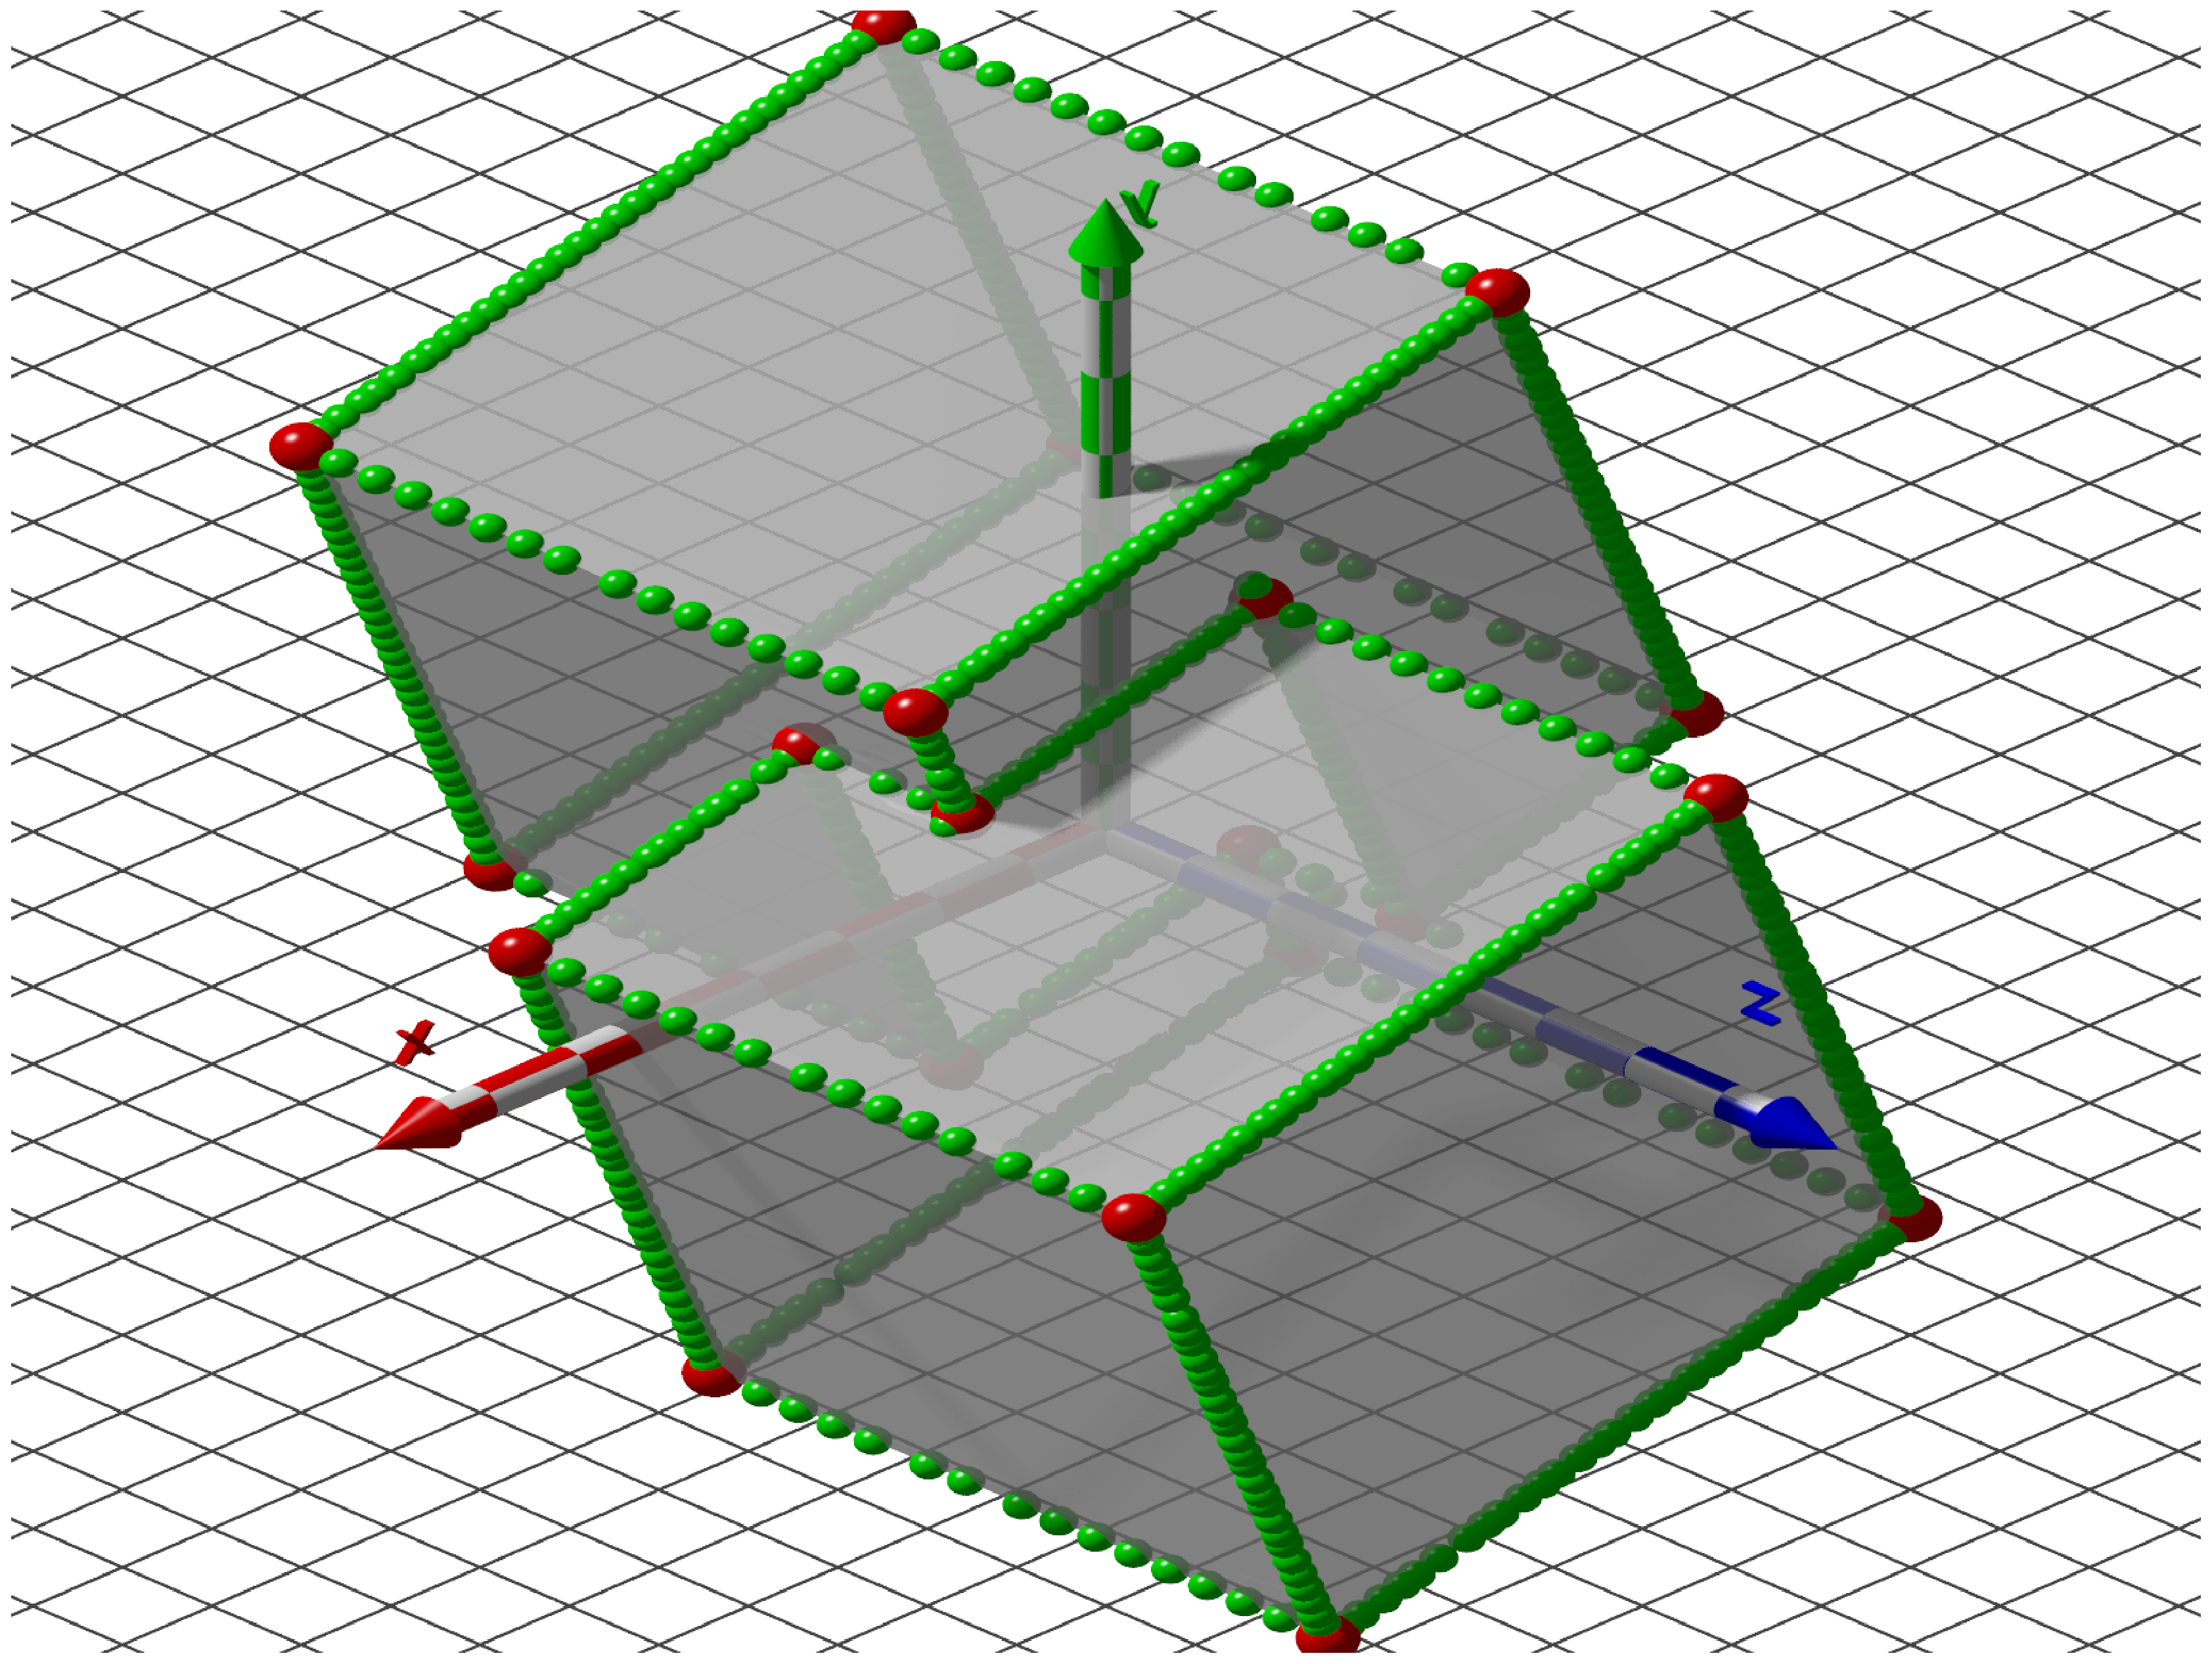
\includegraphics[width=0.2\linewidth]{images/twoCube.B.eps}\label{fig:TwoCube}}
    \subfloat[Flange]{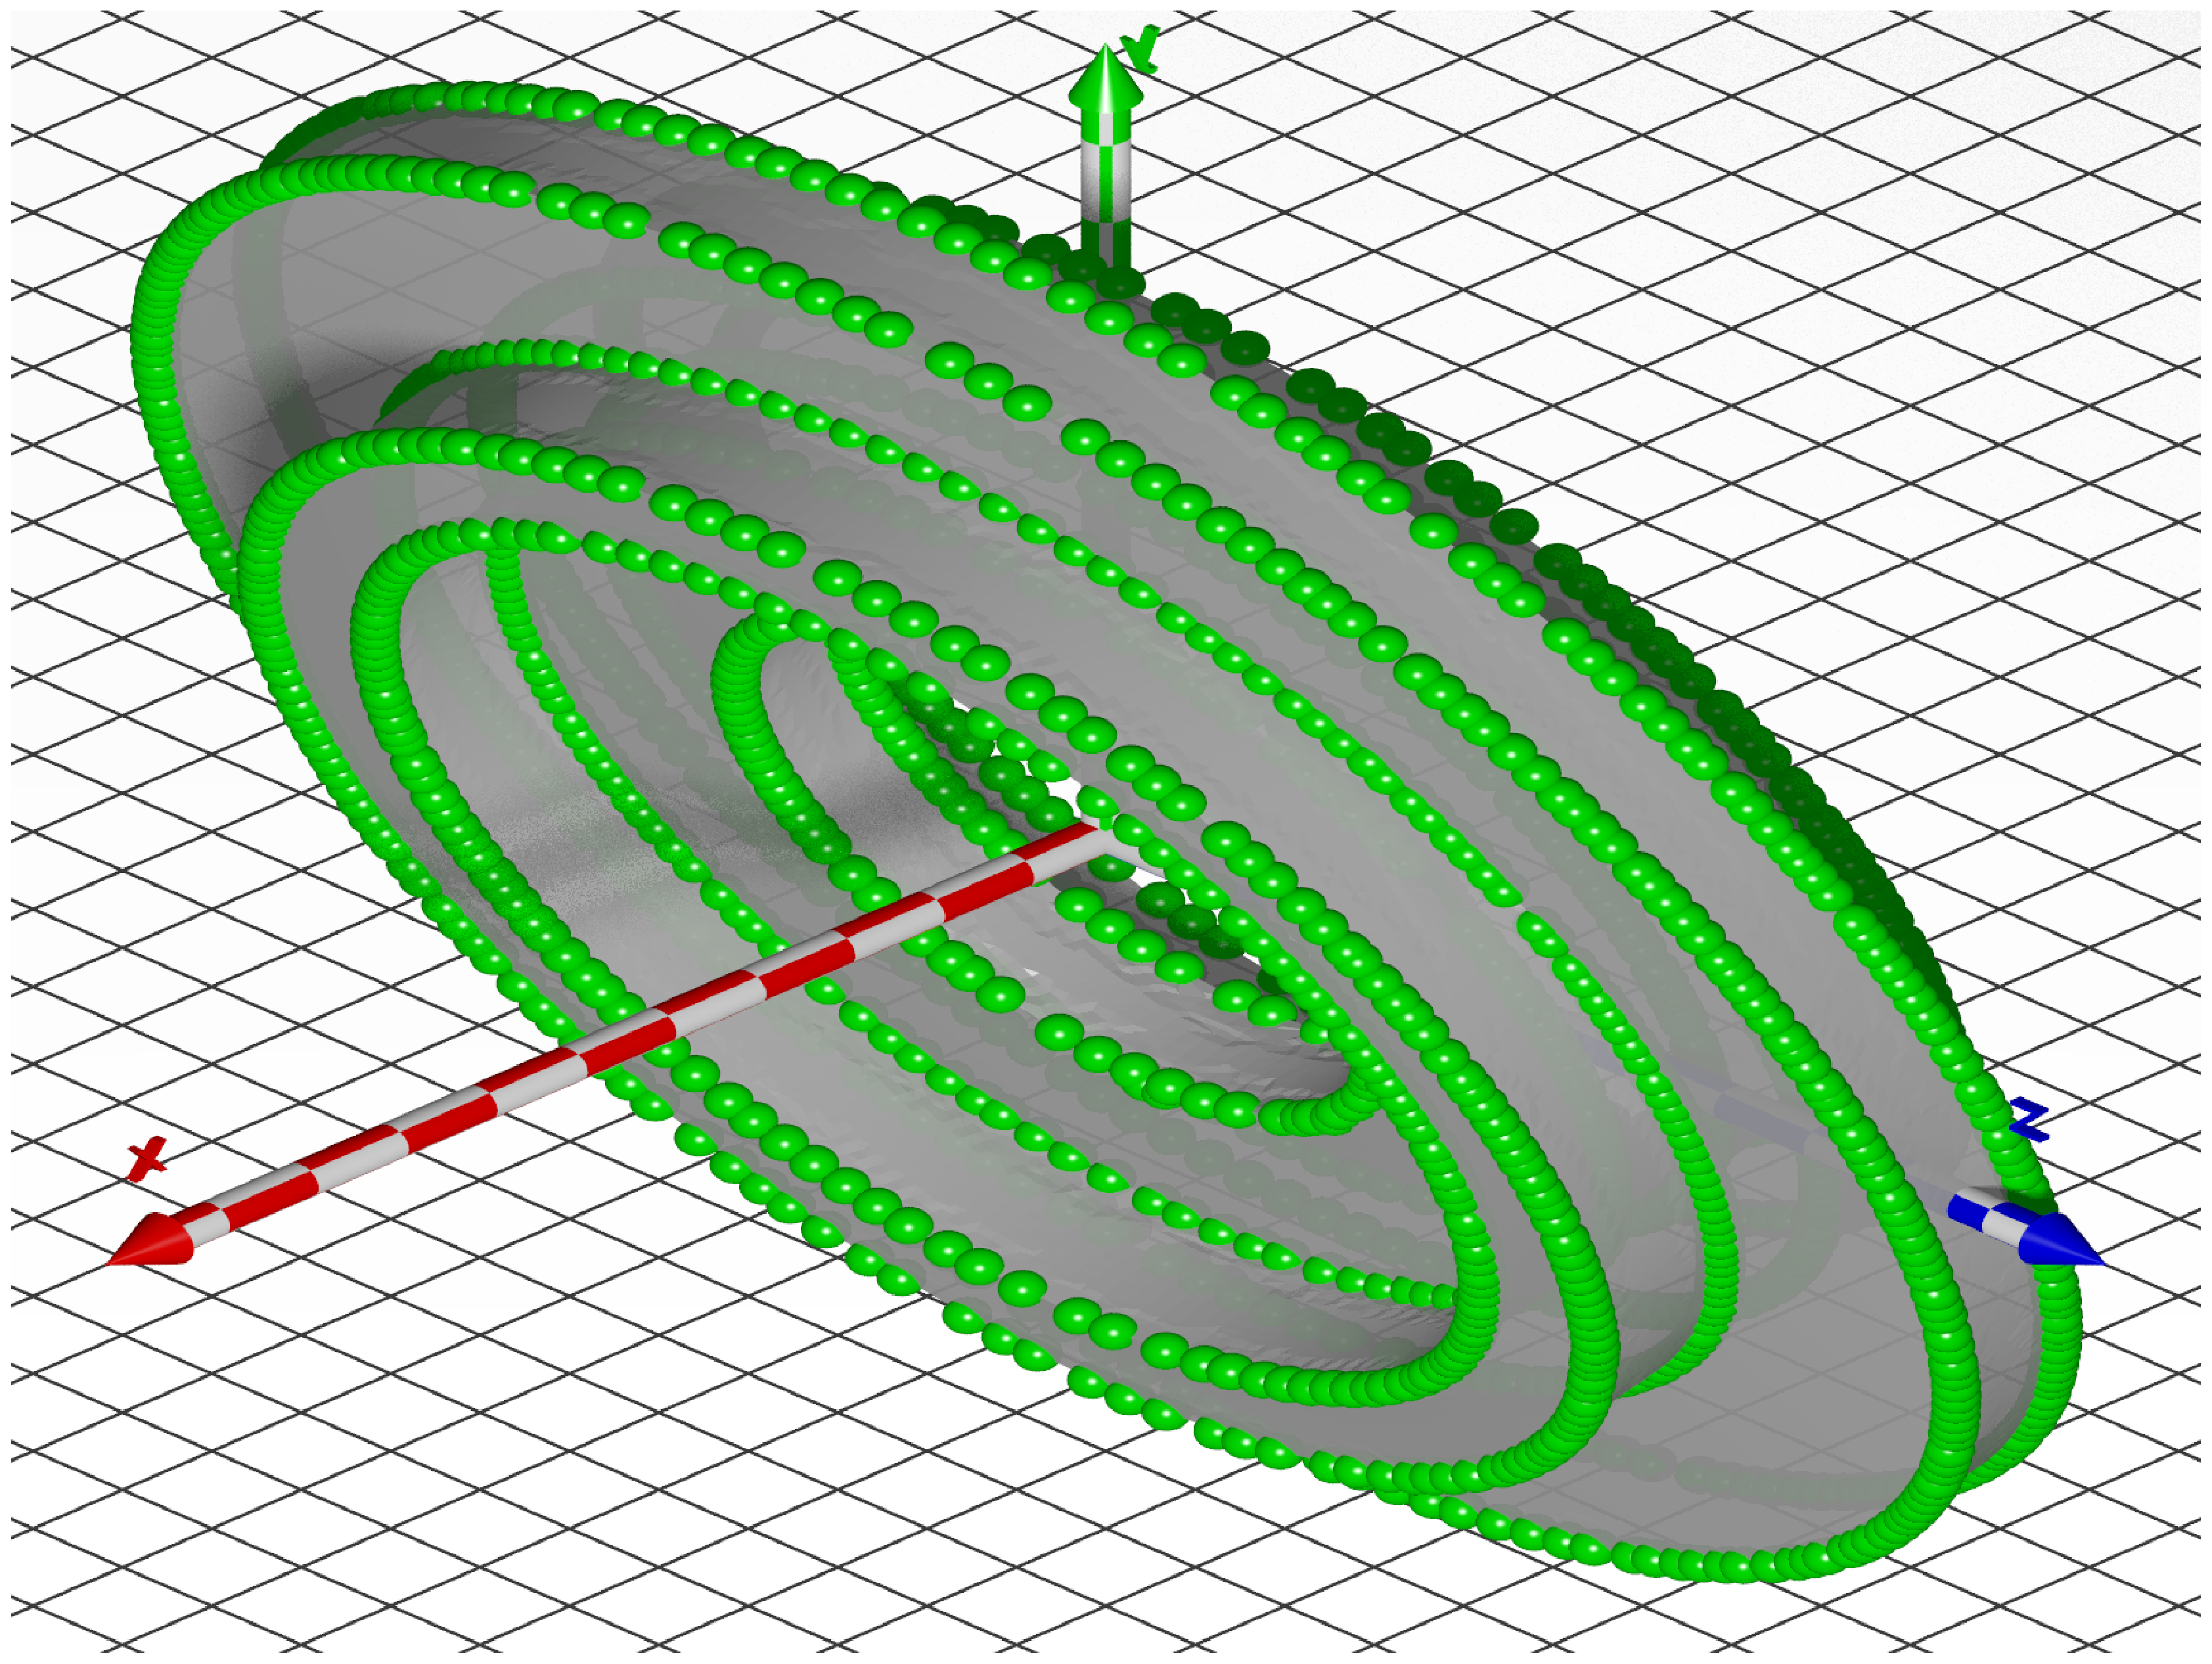
\includegraphics[width=0.2\linewidth]{images/flange.C2.new.eps}\label{fig:flange}}
    \subfloat[Annulus]{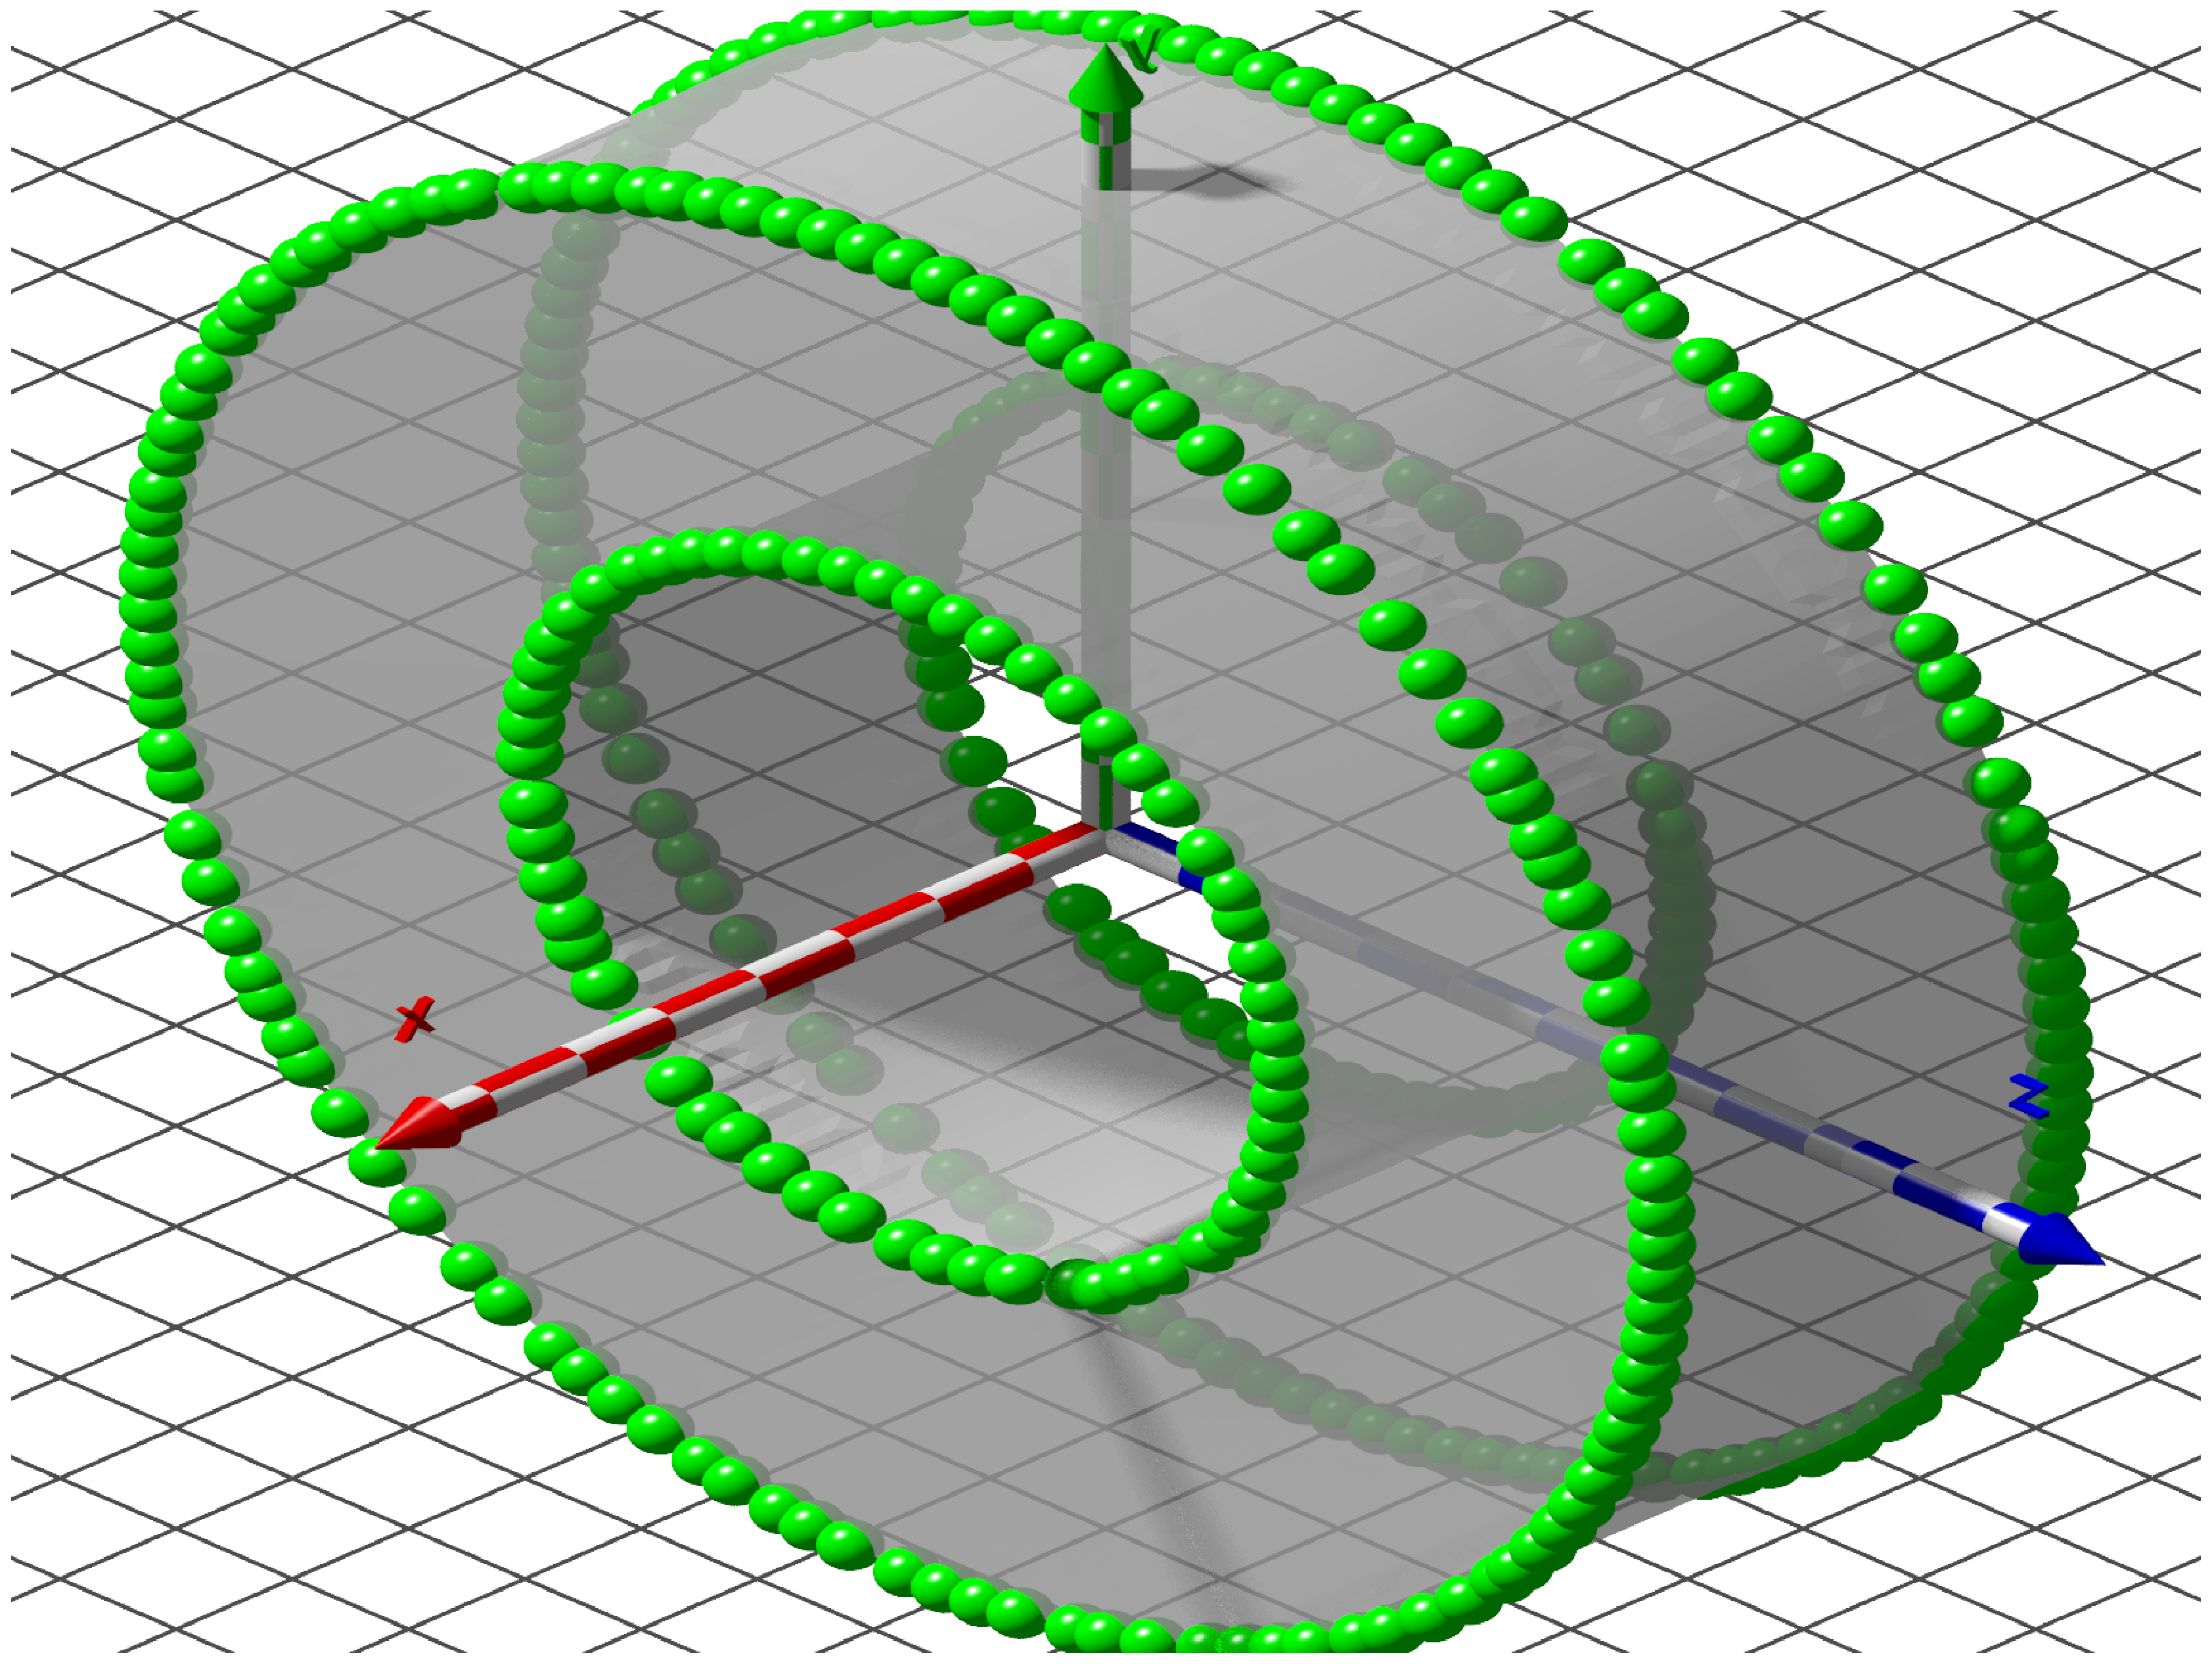
\includegraphics[width=0.2\linewidth]{images/annulus.eps}\label{fig:annulus}}
    \subfloat[Cone]{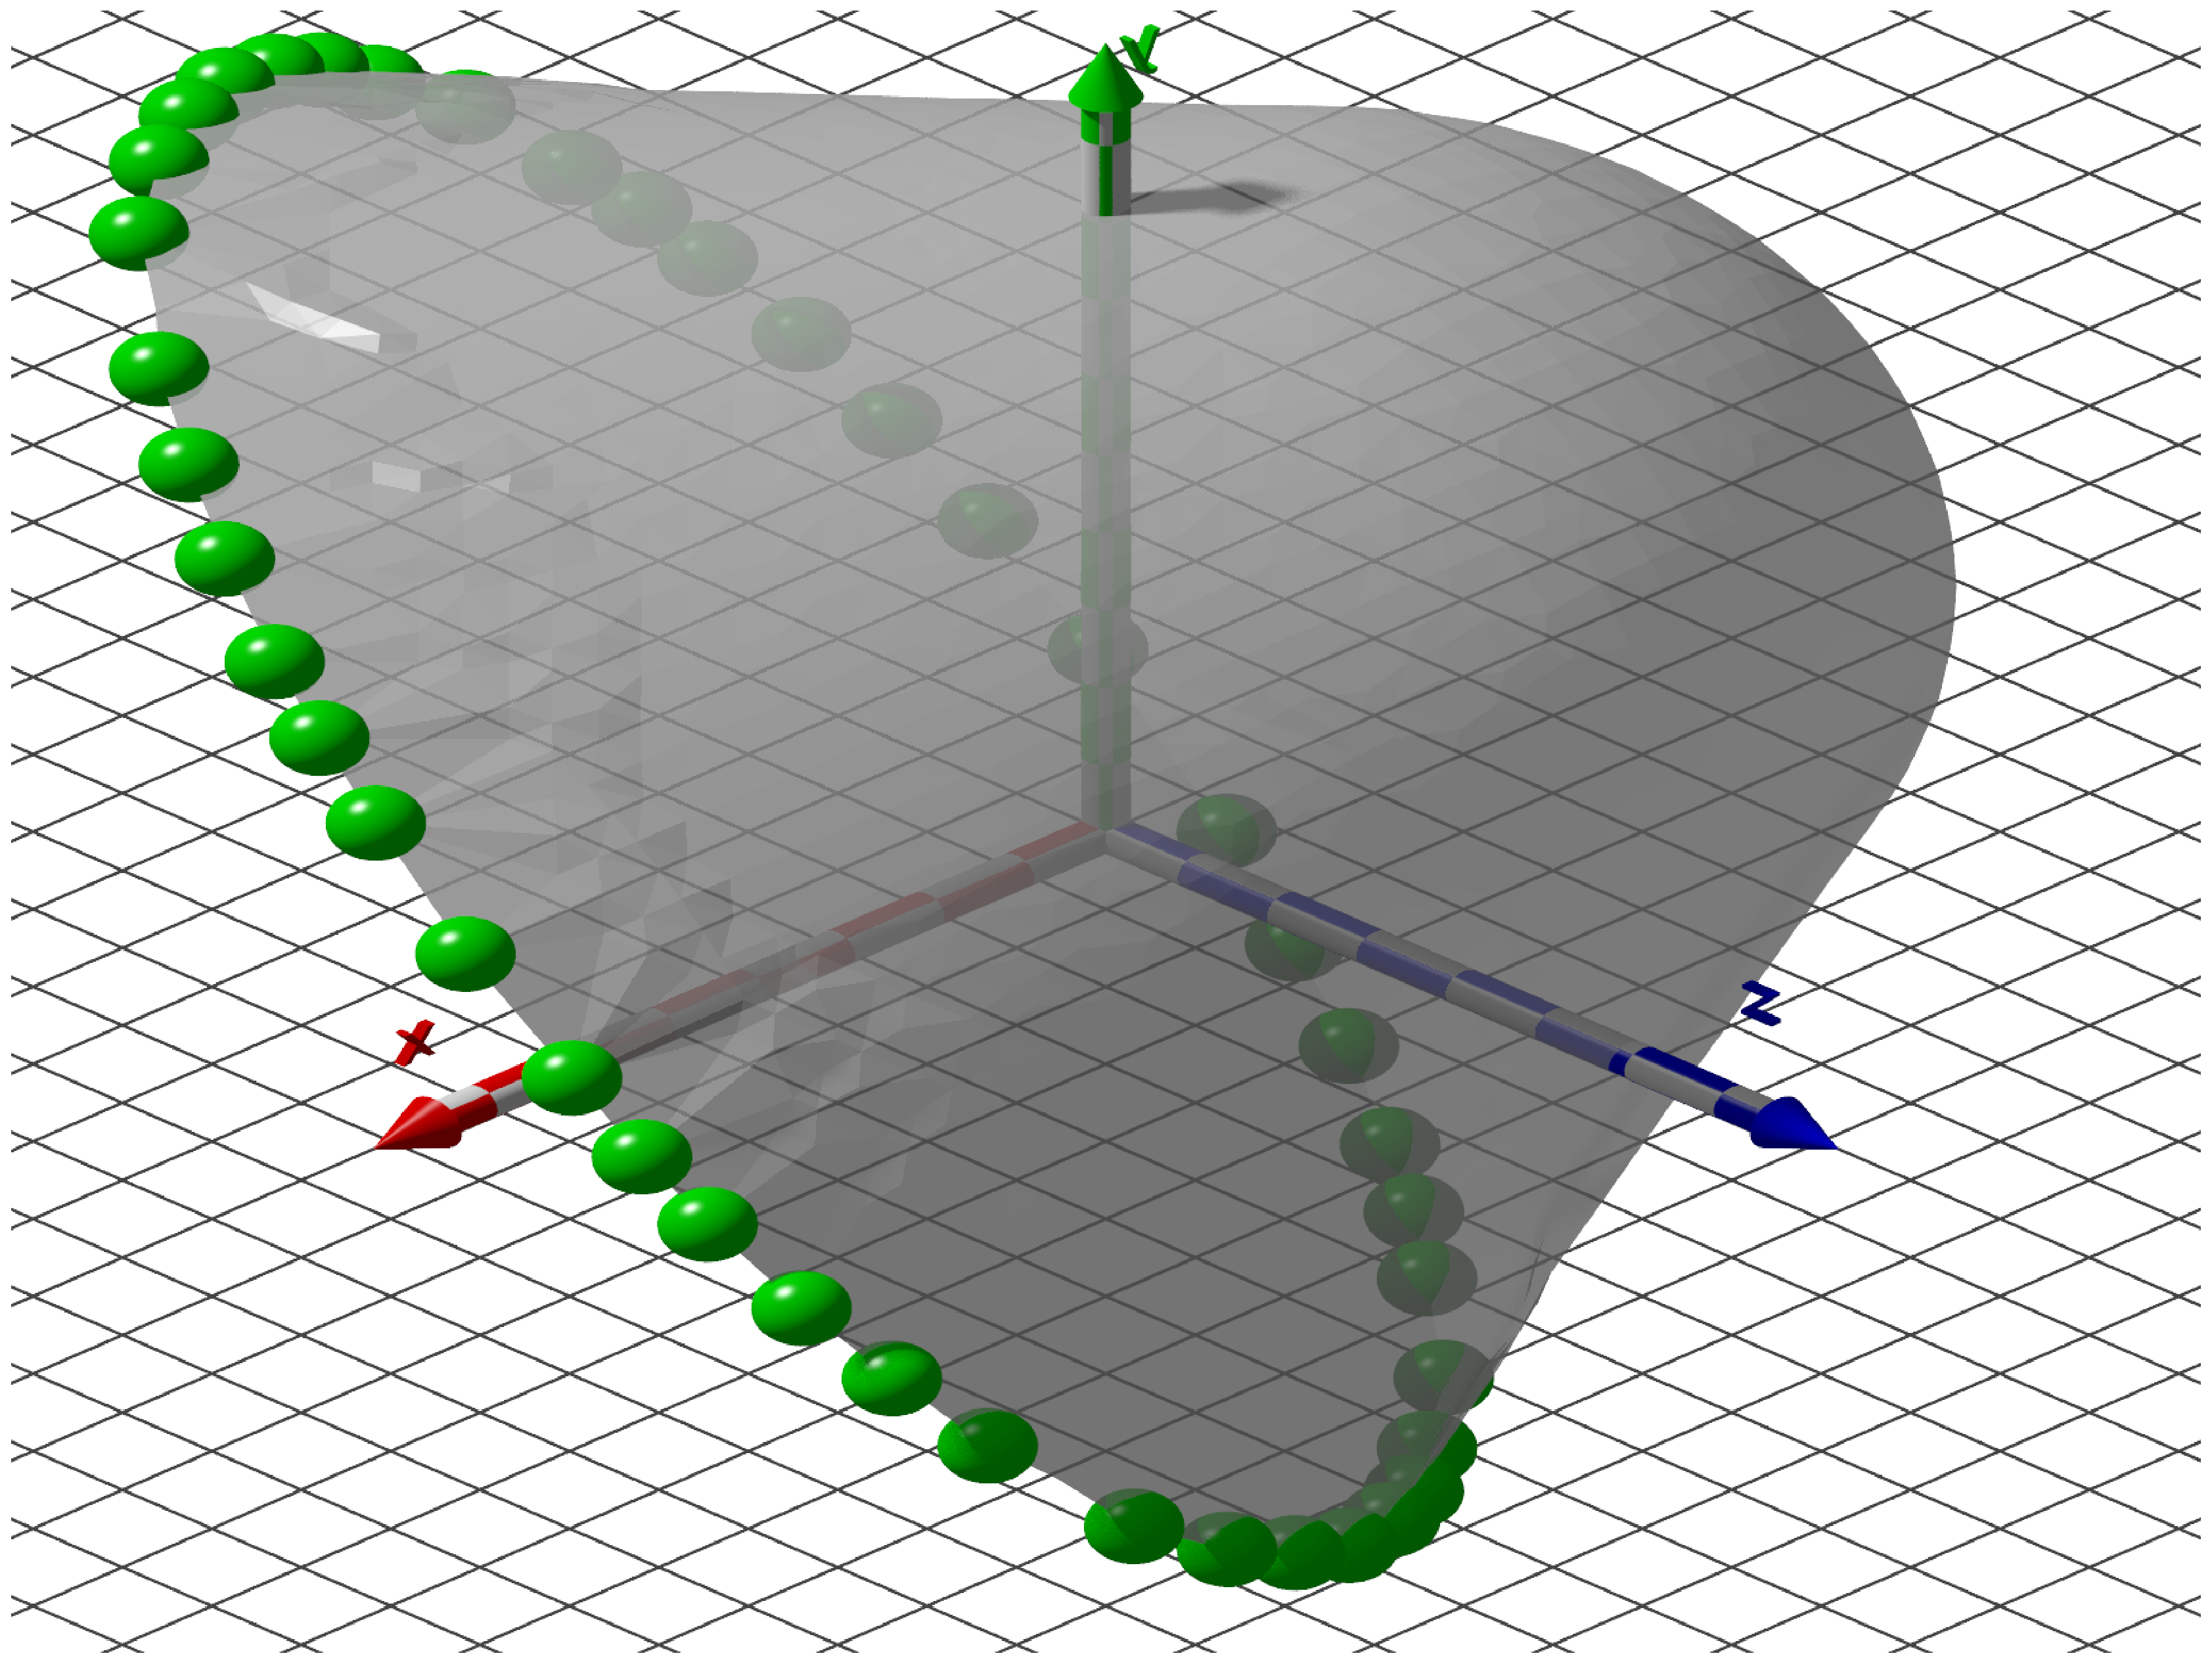
\includegraphics[width=0.2\linewidth]{images/cone.eps}\label{fig:cone}}
    \subfloat[Cannon]{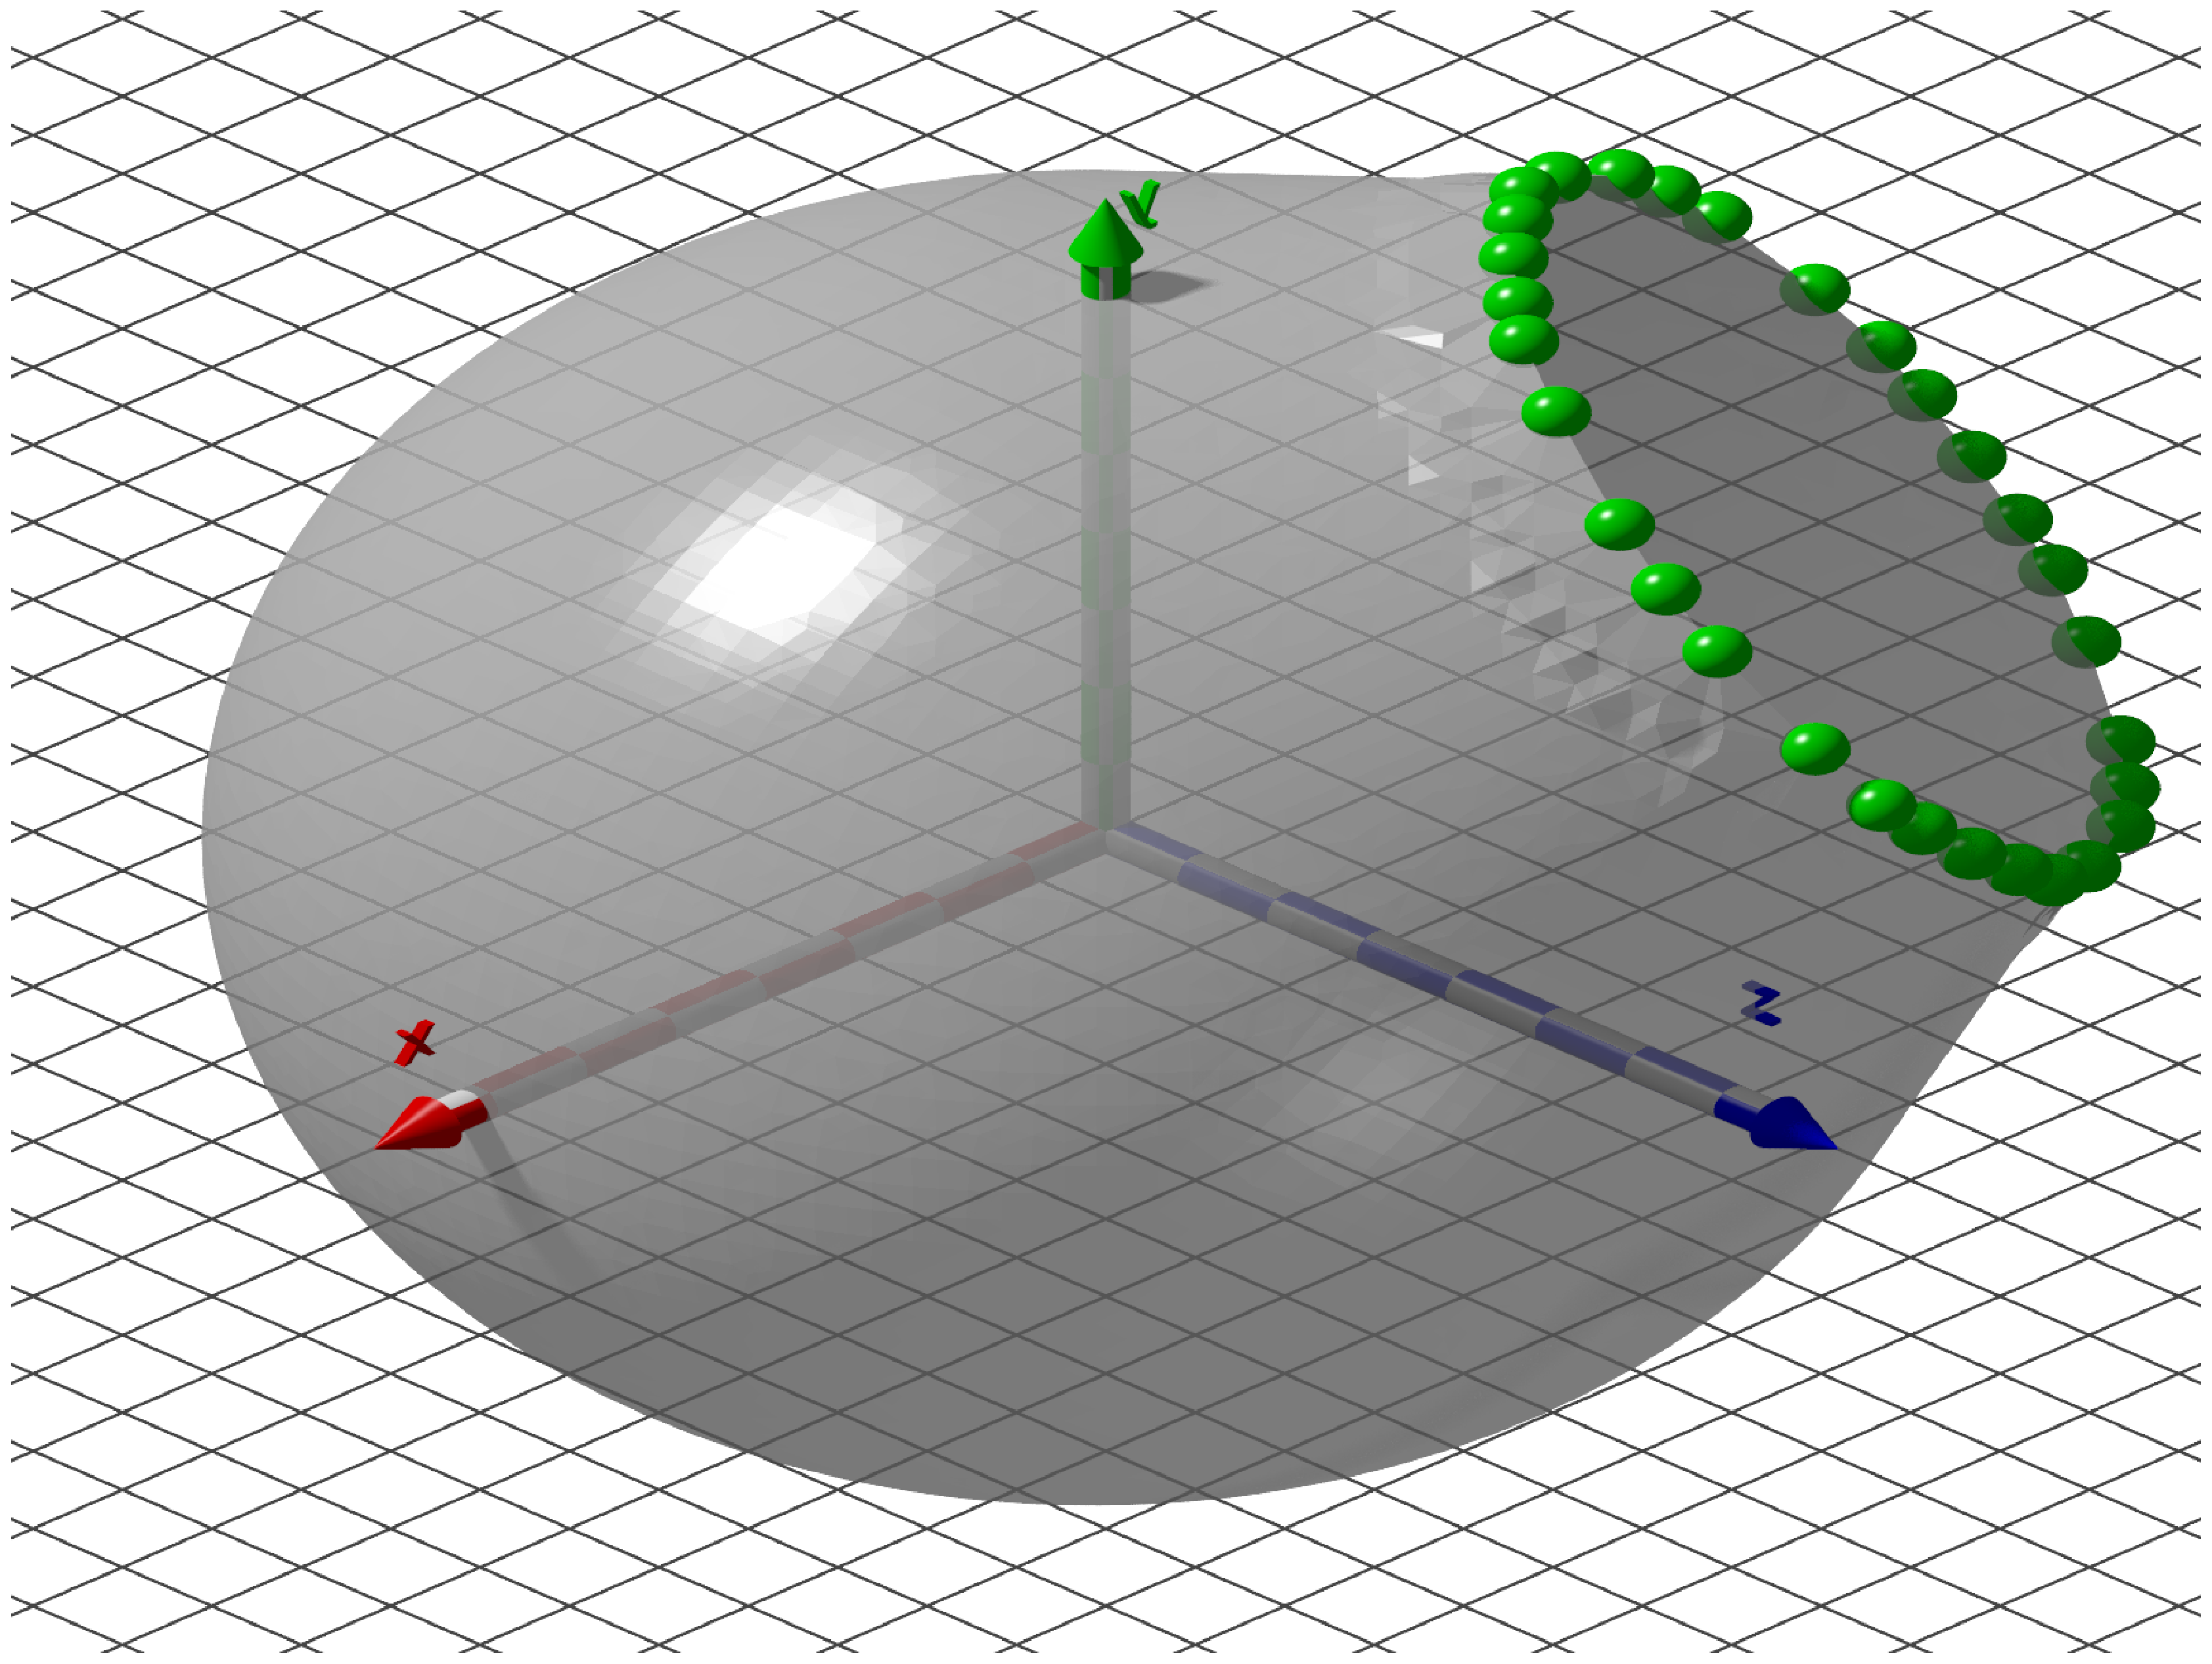
\includegraphics[width=0.2\linewidth]{images/cannon.eps}\label{fig:cannon}}
    \caption{Sharp isosurface mesh and features generated by our algorithm. Sparse edge features are in green and corners in red.}
    \label{fig:SynData}
    
}

%% Uncomment below to disable the manuscript note
\renewcommand{\manuscriptnotetxt}{}

%% Copyright space is enabled by default as required by guidelines.
%% It is disabled by the 'review' option or via the following command:
% \nocopyrightspace

%%%%%%%%%%%%%%%%%%%%%%%%%%%%%%%%%%%%%%%%%%%%%%%%%%%%%%%%%%%%%%%%
%%%%%%%%%%%%%%%%%%%%%% START OF THE PAPER %%%%%%%%%%%%%%%%%%%%%%
%%%%%%%%%%%%%%%%%%%%%%%%%%%%%%%%%%%%%%%%%%%%%%%%%%%%%%%%%%%%%%%%%

\renewcommand{\textfraction}{0.2}
\renewcommand{\dbltopfraction}{0.8}	
\renewcommand{\topfraction}{0.8}

\begin{document}

%% The ``\maketitle'' command must be the first command after the
%% ``\begin{document}'' command. It prepares and prints the title block.

%% the only exception to this rule is the \firstsection command
\firstsection{Introduction}

\maketitle

\begin{figure*}
    \centering
            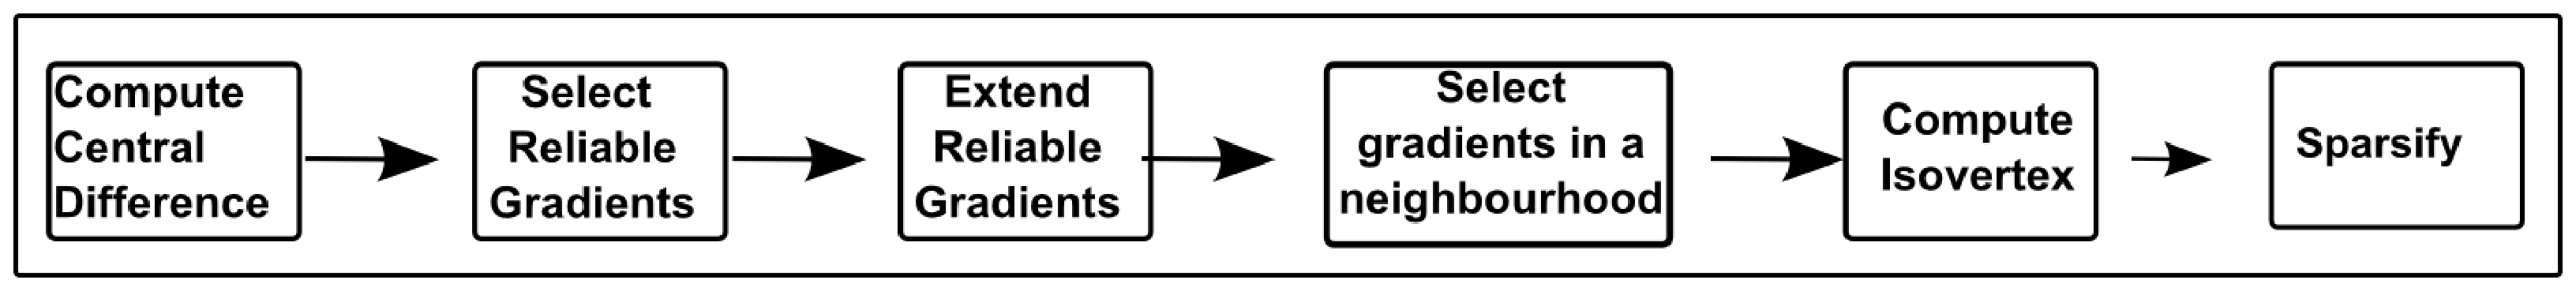
\includegraphics[width=\linewidth]{images/flowchartCrop3.eps}
\caption{Constructing points on sharp features.}
\label{fig:flowchart}
\end{figure*}


\firstsection{Introduction}

X-ray computed tomography (CT) scanners produce regular grids
of scalar values representing material densities of scanned objects.
These scalar values can be modeled as samples of some scalar field
$f:\Rthree \rightarrow \R$.
Object boundaries can be visualized by direct volume rendering
or by visualizing isosurfaces (mesh representations of $f^{-1}(\sigma)$)
representing the object boundaries.
Both approaches have difficulties in representing sharp edges and corners
in the object boundaries.
Sharp edges and corners are best represented
as discontinuities in the gradient field of $f$.
However, standard direct volume rendering 
and isosurface construction algorithms implicitly assume
some continuity in the gradient field of $f$.

In this paper,
we will describe a fast, local algorithm for reliably reconstructing
the gradient field of $f$ 
and constructing points on sharp edges and corners of an isosurface.
The points can be rendered in conjunction with isosurface visualizations
to highlight sharp features or
they can be joined to form a skeleton representation of the sharp feature.
They can also be used as input to isosurface or surface meshing algorithms
which are designed to handle surfaces with sharp features.

Previous algorithms to construct isosurfaces with sharp features
relied upon exact surface normals being provided 
to the algorithm~\cite{
ab-fpmmo-03,gk-eretm-04,hwco-cmsaf-05,jlsw-dchd-02,
kbsh-fssev-01,ms-ispmg-10,Varadhan:2003:fss,sw-dmcpc-04,zhk-dctps-04}.
The algorithm in~\cite{bw-cisec-13}
constructs isosurfaces with sharp features
from gradient grid data
where gradients are provided at each grid vertex.
We know of no work on constructing isosurfaces with sharp features
directly from scalar data.

If the level set $f^{-1}(\sigma)$ of a scalar field
$f:\Rthree \rightarrow \R$ has sharp features,
then there are discontinuities in the gradients of $f$
at the sharp features.
Constructing the gradients near those discontinuities
is difficult.
Formulas for approximating gradients
such as the central difference formula~\cite{ck-nmc-07}
or higher order approximations~\cite{aml-ger-10,ham-thqge-11,mmmy-cnes-97}
assume the gradient is continuous at the given location.
Anisotropic diffusion~\cite{
bx-adsfs-03,cdr-agdsp-00,twbo-gssad-02,twbo-gspnm-03,tw-adsnf-03} 
removes noise in low curvature regions of the scalar field 
without affecting high curvature regions,
but it does not produce correct gradients near gradient discontinuities.

Instead of attempting to produce correct gradients at all grid vertices,
our algorithm identifies correct gradients 
and uses only those gradients to predict locations
of isosurface vertices.
We give an algorithm for identifying correct gradients
based on their agreement with neighboring gradients.
The algorithm produces enough correct gradients in the neighborhood
of sharp features to generate points on those sharp features.

The basic steps of our algorithm are given in Figure~\ref{fig:flowchart}.
The first two steps produce a set of reliable gradients.
The algorithm then selects a set of reliable gradients around each cube,
computes a set of isosurface tangent planes from those gradients,
and finds a point at the ``intersection'' of those tangent planes.
It simultaneously identifies whether that point lies 
on a sharp edge or corner of the isosurface
or on a smooth region of the isosurface.
The algorithm sparsifies the set of isosurface vertices on sharp features
and returns the sparsified set.
The sparsified set can be used for generating an isosurface mesh
using feature preserving algorithms such as MergeSharp~\cite{bw-cisec-13}
or Weighted Cocone~\cite{dgqsww-fprss-12}.
Alternatively, it can be used to construct a representative sharp
feature curve or can be rendered directly to highlight sharp features
on the isosurface.

The focus of this paper is on constructing a set of reliable gradients
from scalar data in the presence of gradient discontinuities.
As part of our work, we developed a theory (Section~\ref{sec:gradients} 
giving bounds on gradient approximation errors
based on comparing gradients to nearby gradients.

There is a substantial amount of work on computing surfaces 
with sharp features from point cloud data.
Some of the proposed algorithms (e.g. \cite{dgqsww-fprss-12,sym-fpmg-10})
compute points on sharp features
and then create representative curves from those points.
Scalar data might be turned into point cloud data 
by computing a set of points which approximate the
intersection of the isosurface and the grid edges.
Any of the point cloud algorithms which reconstruct sharp features 
or surfaces with sharp features can then be applied to this point cloud data.

We strongly believe that there is a big advantage in constructing sharp features
directly from scalar data without (the extra step of) converting it to point cloud data.
First, converting scalar data to point cloud data ignores the grid structure
of the scalar data.
This grid structure can be employed both for constructing sharp features
and for meshing those features. Generally, grid based methods are faster than their point-cloud counterparts.
Second, point cloud data is extremely noisy so the point cloud 
reconstruction algorithms average over \textit{large} neighborhoods.
It is extremely difficult to predict the results of the algorithms
or to guarantee that the algorithms are not ignoring features in the data.
In contrast, our algorithm runs over a small, local neighborhood,
so that all features of the data (for better or for worse) are represented in the output.
Finally, because our algorithm is local,
it is very fast and easily parallelizable.

Our research contributions in this paper are:
\begin{enumerate}
\itemsep0em 
\item An algorithm for constructing reliable gradients
from scalar data in the presence of gradient discontinuities.
\item Proofs of bounds on the angle between the approximate gradients
and the true gradients.
\end{enumerate}
We use our algorithm to:
\begin{enumerate}
\itemsep0em
\item Construct samples points on sharp edges and corners of an isosurface.
\item Construct isosurface meshes with good representations of sharp edges and corners.
\end{enumerate}

We note that the algorithm for constructing the reliable gradients and the sample points
is completely local, and thus fast and easily parallelizable.








\section{Related Work}

Algorithms for constructing isosurfaces with sharp features
are given
in~\cite{ab-fpmmo-03,hwco-cmsaf-05,jlsw-dchd-02,kbsh-fssev-01,
ms-ispmg-10,sw-dcss-02,sw-dmcpc-04,Varadhan:2003:fss,zhk-dctps-04}.
All these algorithms require
exact surface normals as part of the input.

\MergeSharp~\cite{bw-cisec-13} is an algorithm
for constructing isosurfaces with sharp features from gradient data.
Input to the algorithm is gradient grid data,
scalar values and gradient vectors at each vertex of a regular grid.
The algorithm can handle noise in the gradient vectors 
and missing gradient vectors.

Salman et al.~\cite{sym-fpmg-10} and Dey et al.~\cite{dgqsww-fprss-12}
reconstructed piecewise smooth surfaces with sharp features 
from point cloud data
by separately placing mesh vertices on the sharp features
and vertices inside the smooth patches.
They place ``protecting ball'' around mesh vertices on sharp features
so that no vertices inside the smooth patches are placed 
near the sharp features.
Algorithm \MergeSharp does something similar,
merging grid cubes around sharp features so that isosurface vertices
on sharp features are ``isolated'' away from other vertices.

Fleishman et al.~\cite{fcs-rmlsf-2005} introduced a least-squares technique to reconstruct a piecewise smooth surface. The sharp features are reconstructed as intersection of these smooth regions. Oztireli et al.~\cite{Oeztireli2009} extended the moving least square reconstruction to sharp features using kernel regression. The strength of robust kernel regression, makes this method robust to noise. Avron et al.~\cite{avron2010L} used a l1-sparse approach to reconstruct sharp features from point set.

Formulas for improving the numerical accuracy of gradient computations
from scalar data
are given in~\cite{aml-ger-10,ham-thqge-11,mmmy-cnes-97}.
These formulas assume the gradient vector field is smooth
and do not work when there are discontinuities in the vector field.
They also do not work when there is noise in the input scalar data.

Anisotropic diffusion is a technique by which the filtering
of surface normals or field gradients changes based on local curvature.
Gradients or normals in low curvature regions are moved to agree 
with their neighbors.
Gradients or normals in high curvature regions are moved only slightly.
Anisotropic diffusion for mesh smoothing is described
in~\cite{bx-adsfs-03,cdr-agdsp-00,twbo-gssad-02,twbo-gspnm-03}.
Tasziden et. al.~\cite{tw-adsnf-03} used anisotropic diffusion 
to preserve features in isosurface reconstruction.

Features in papers on anisotropic diffusion are high curvature regions,
not regions with normal or gradient discontinuities (infinite curvature.)
Anisotropic diffusion applied to surfaces or gradient fields
with discontinuities will filter noise from smooth regions,
but it will not improve estimations at discontinuities
or assist in identifying such discontinuities.


\begin{figure}
	\begin{center}
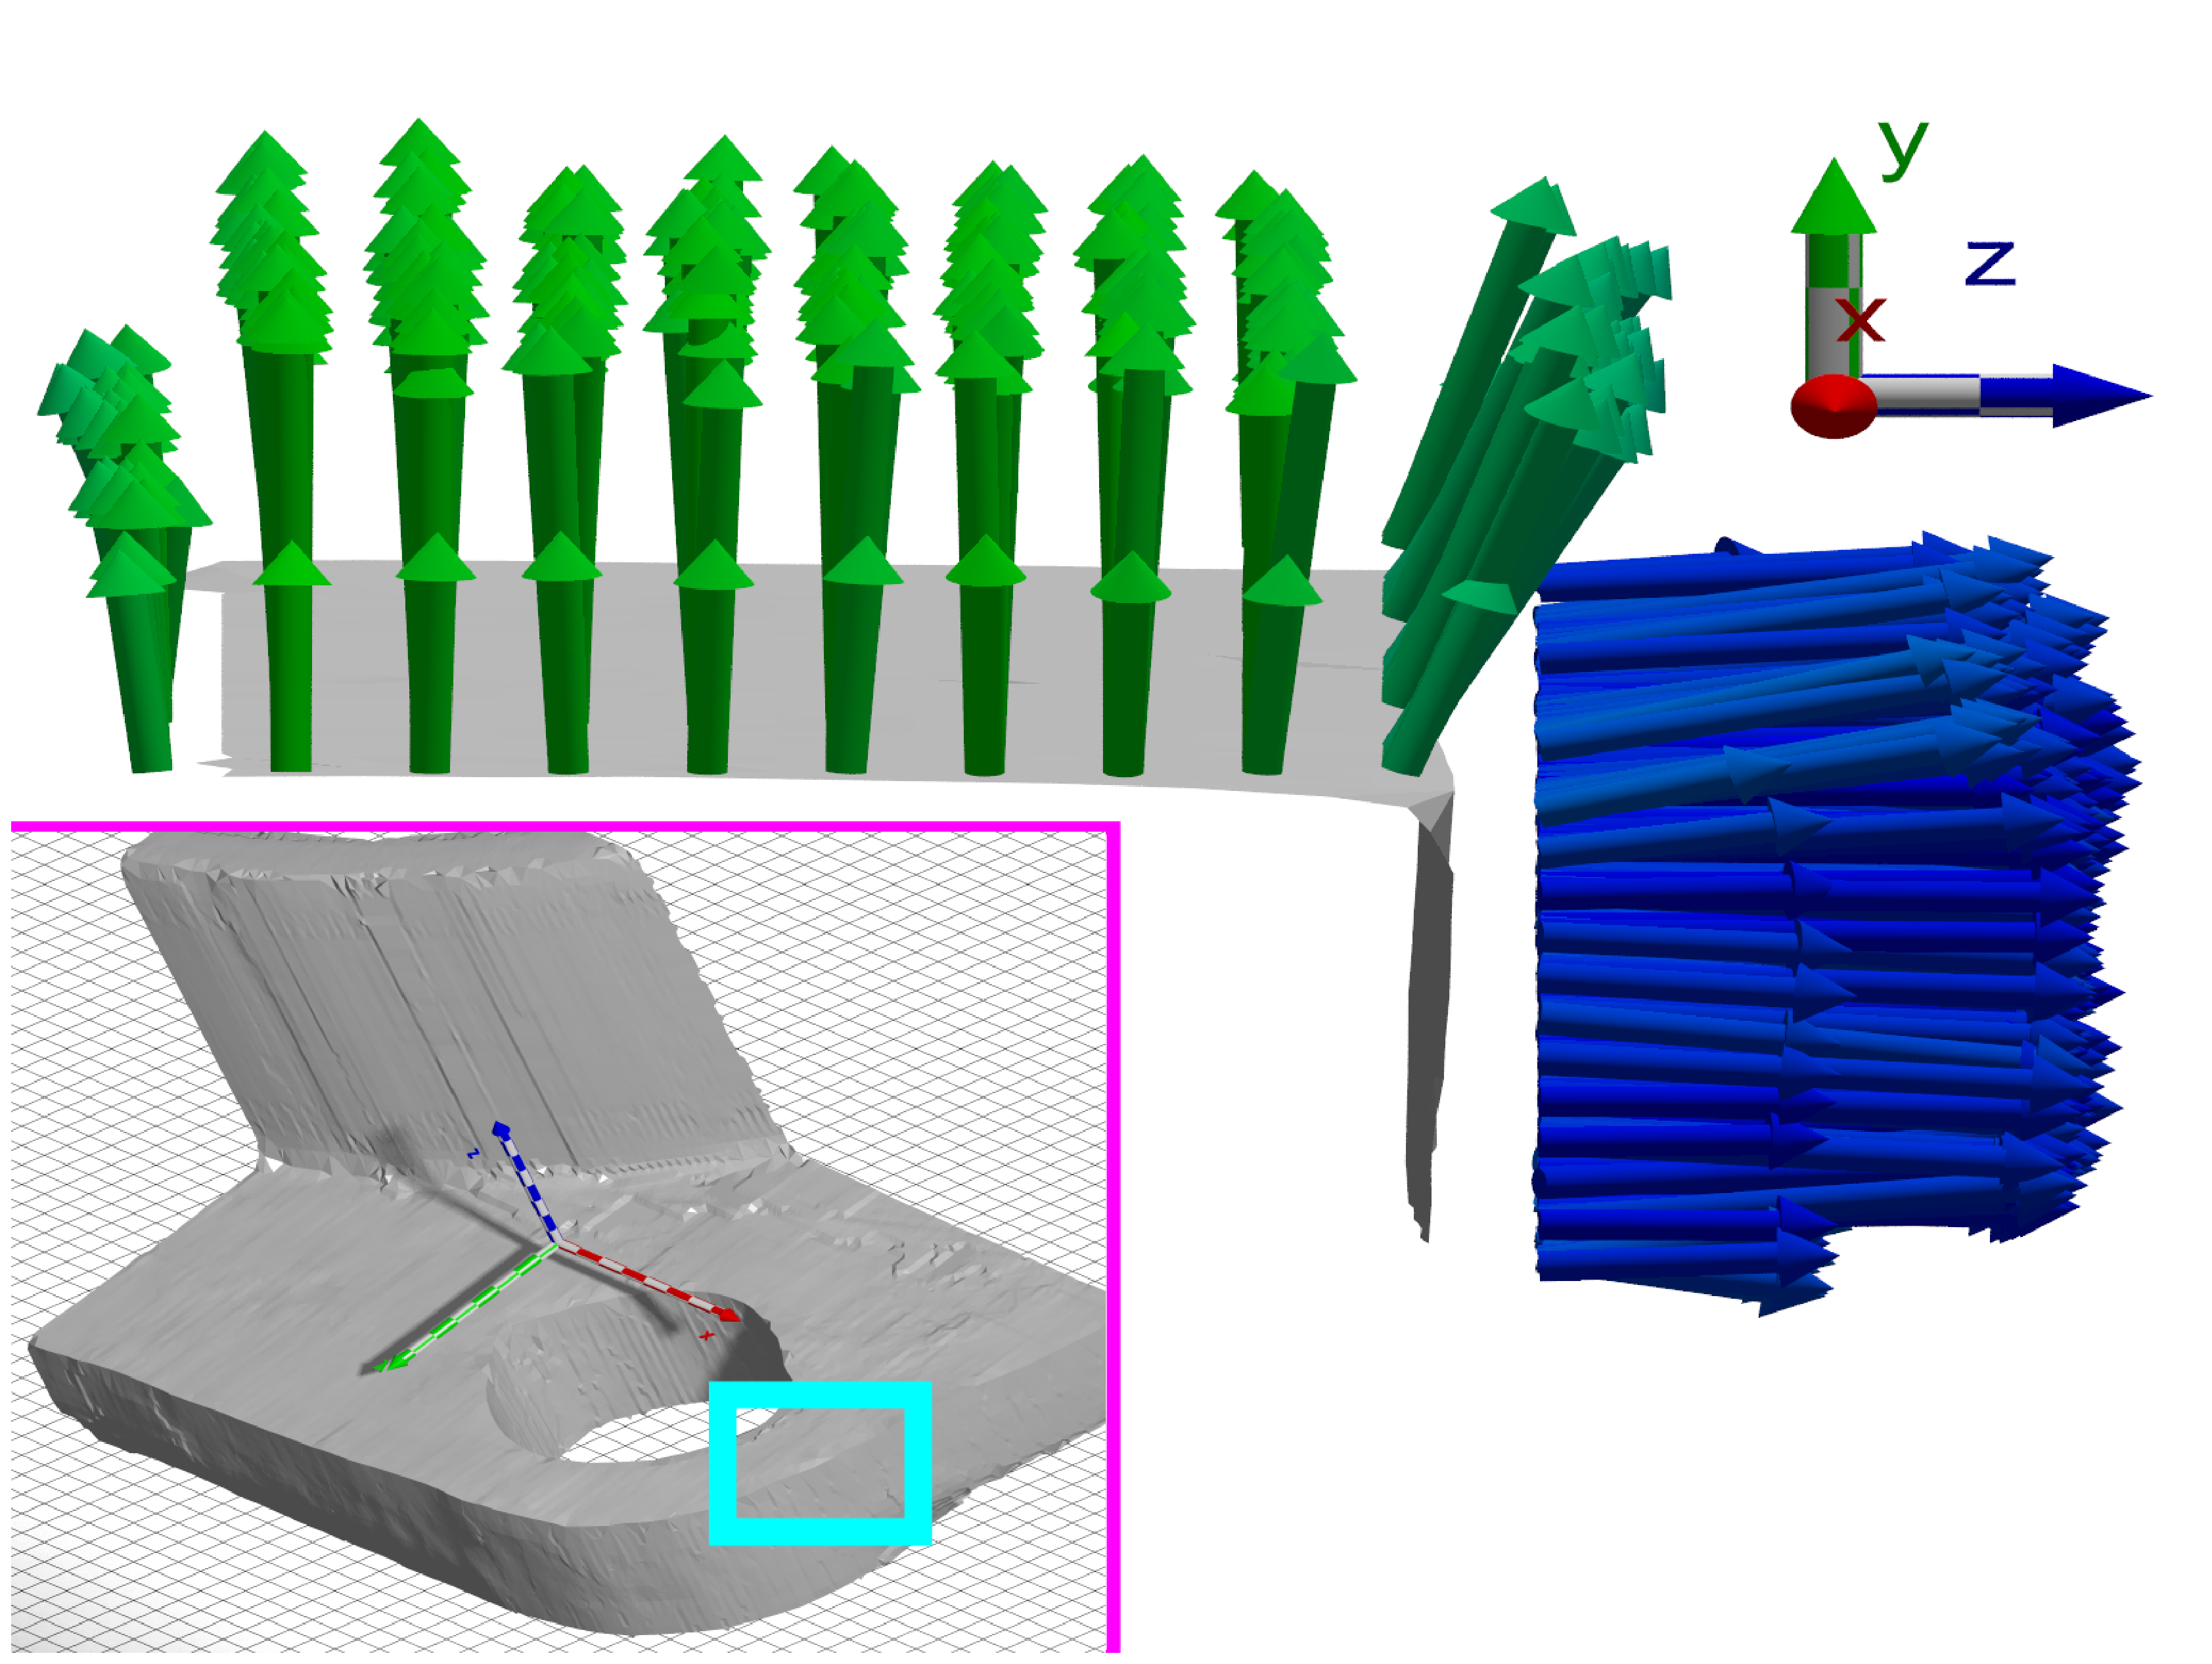
\includegraphics[width=0.5\linewidth]{images/setA.crop2.cdiff.new.eps}
	\caption{Gradient computation around a sharp surface edge in a CT data.
        Expanded view of the cyan rectangle, shows the central difference gradients at grid vertices which intersect the isosurface. Those parallel to Y axis are colored green, those parallel to Z are colored blue, the rest are linearly interpolated. The central difference formula produces incorrect gradients near the sharp edge. Gradients which are not near the sharp
        edge are correct.}
	\label{fig:grad-1}
    \end{center}
\end{figure}
\begin{figure}
	\centering
  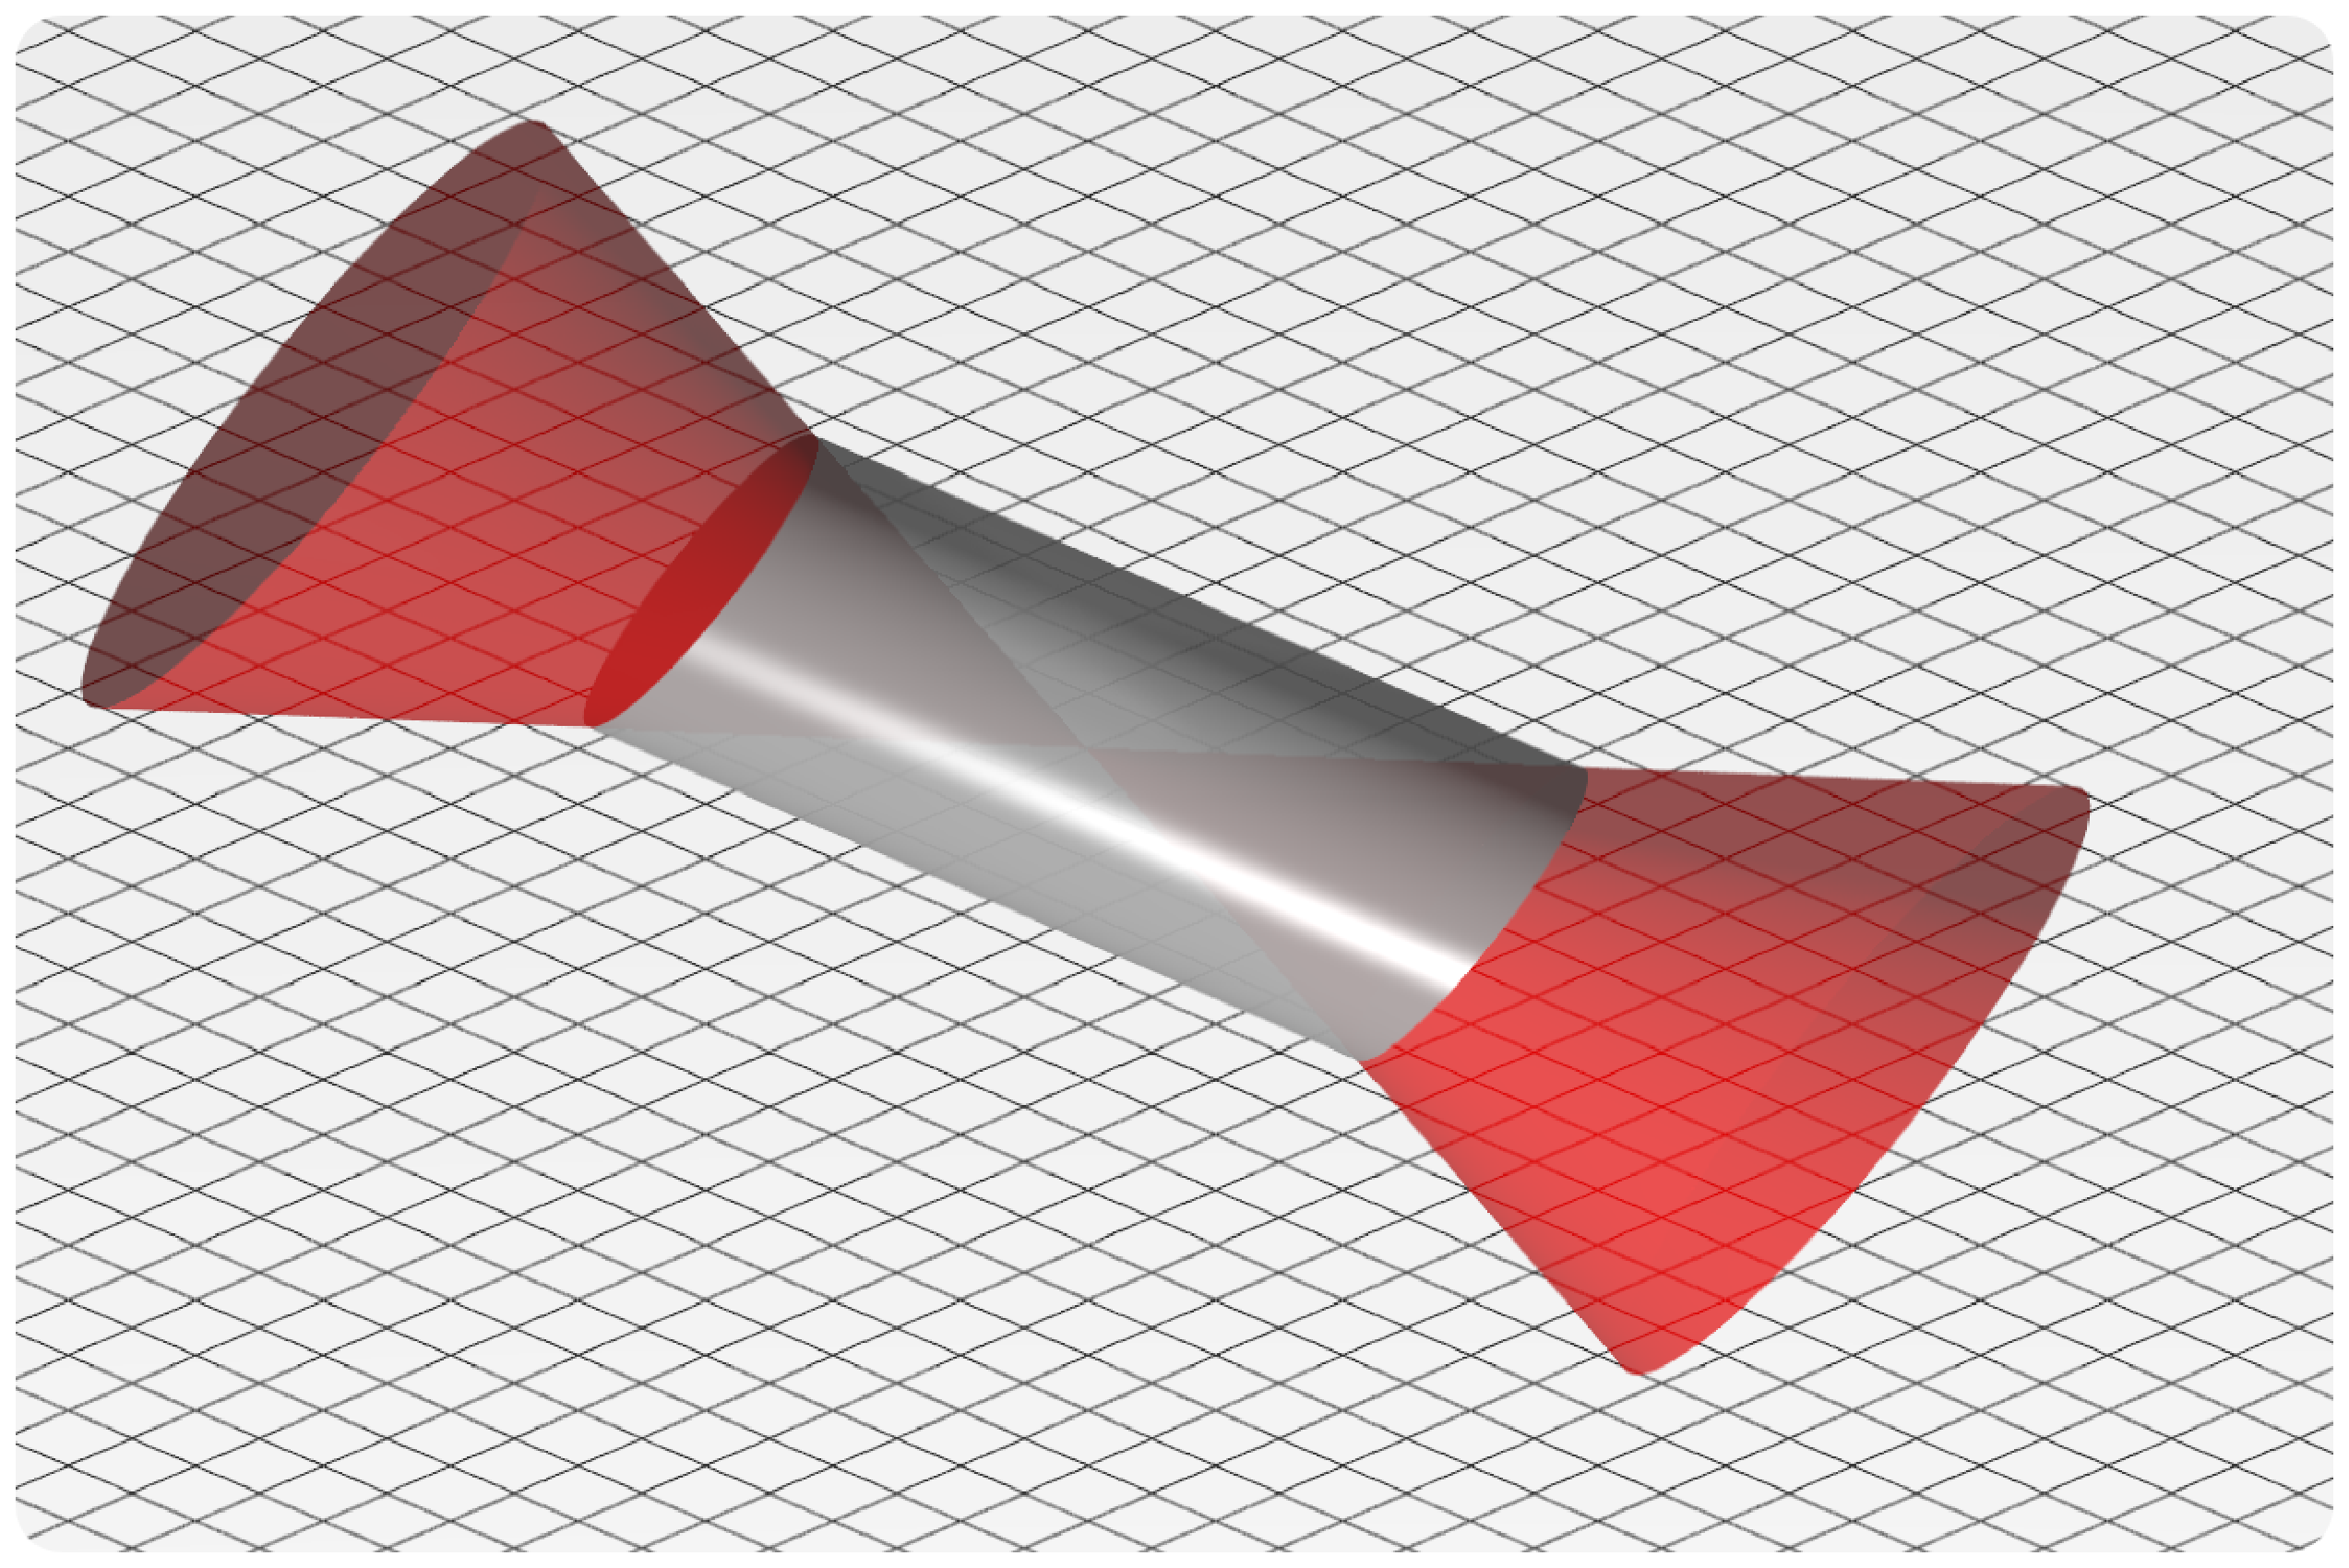
\includegraphics[width=0.5\linewidth]{images/2cone.eps}
  \caption{A double cone (red) representing the gradient discontinuities
 of a scalar field $f$.
 The field $f$ is the maximum of the distance to a line 
 and to a plane orthogonal to that line.
 The isosurfaces of $f$ are boundaries of cylinders.
 A sample isosurface is shown in grey.
 The double cone separates $\Rthree$ into three regions.
 The field $f$ is continuous within each region.}
	\label{fig:double_cone}
\end{figure}

%\begin{figure}[t]
%\begin{center}
%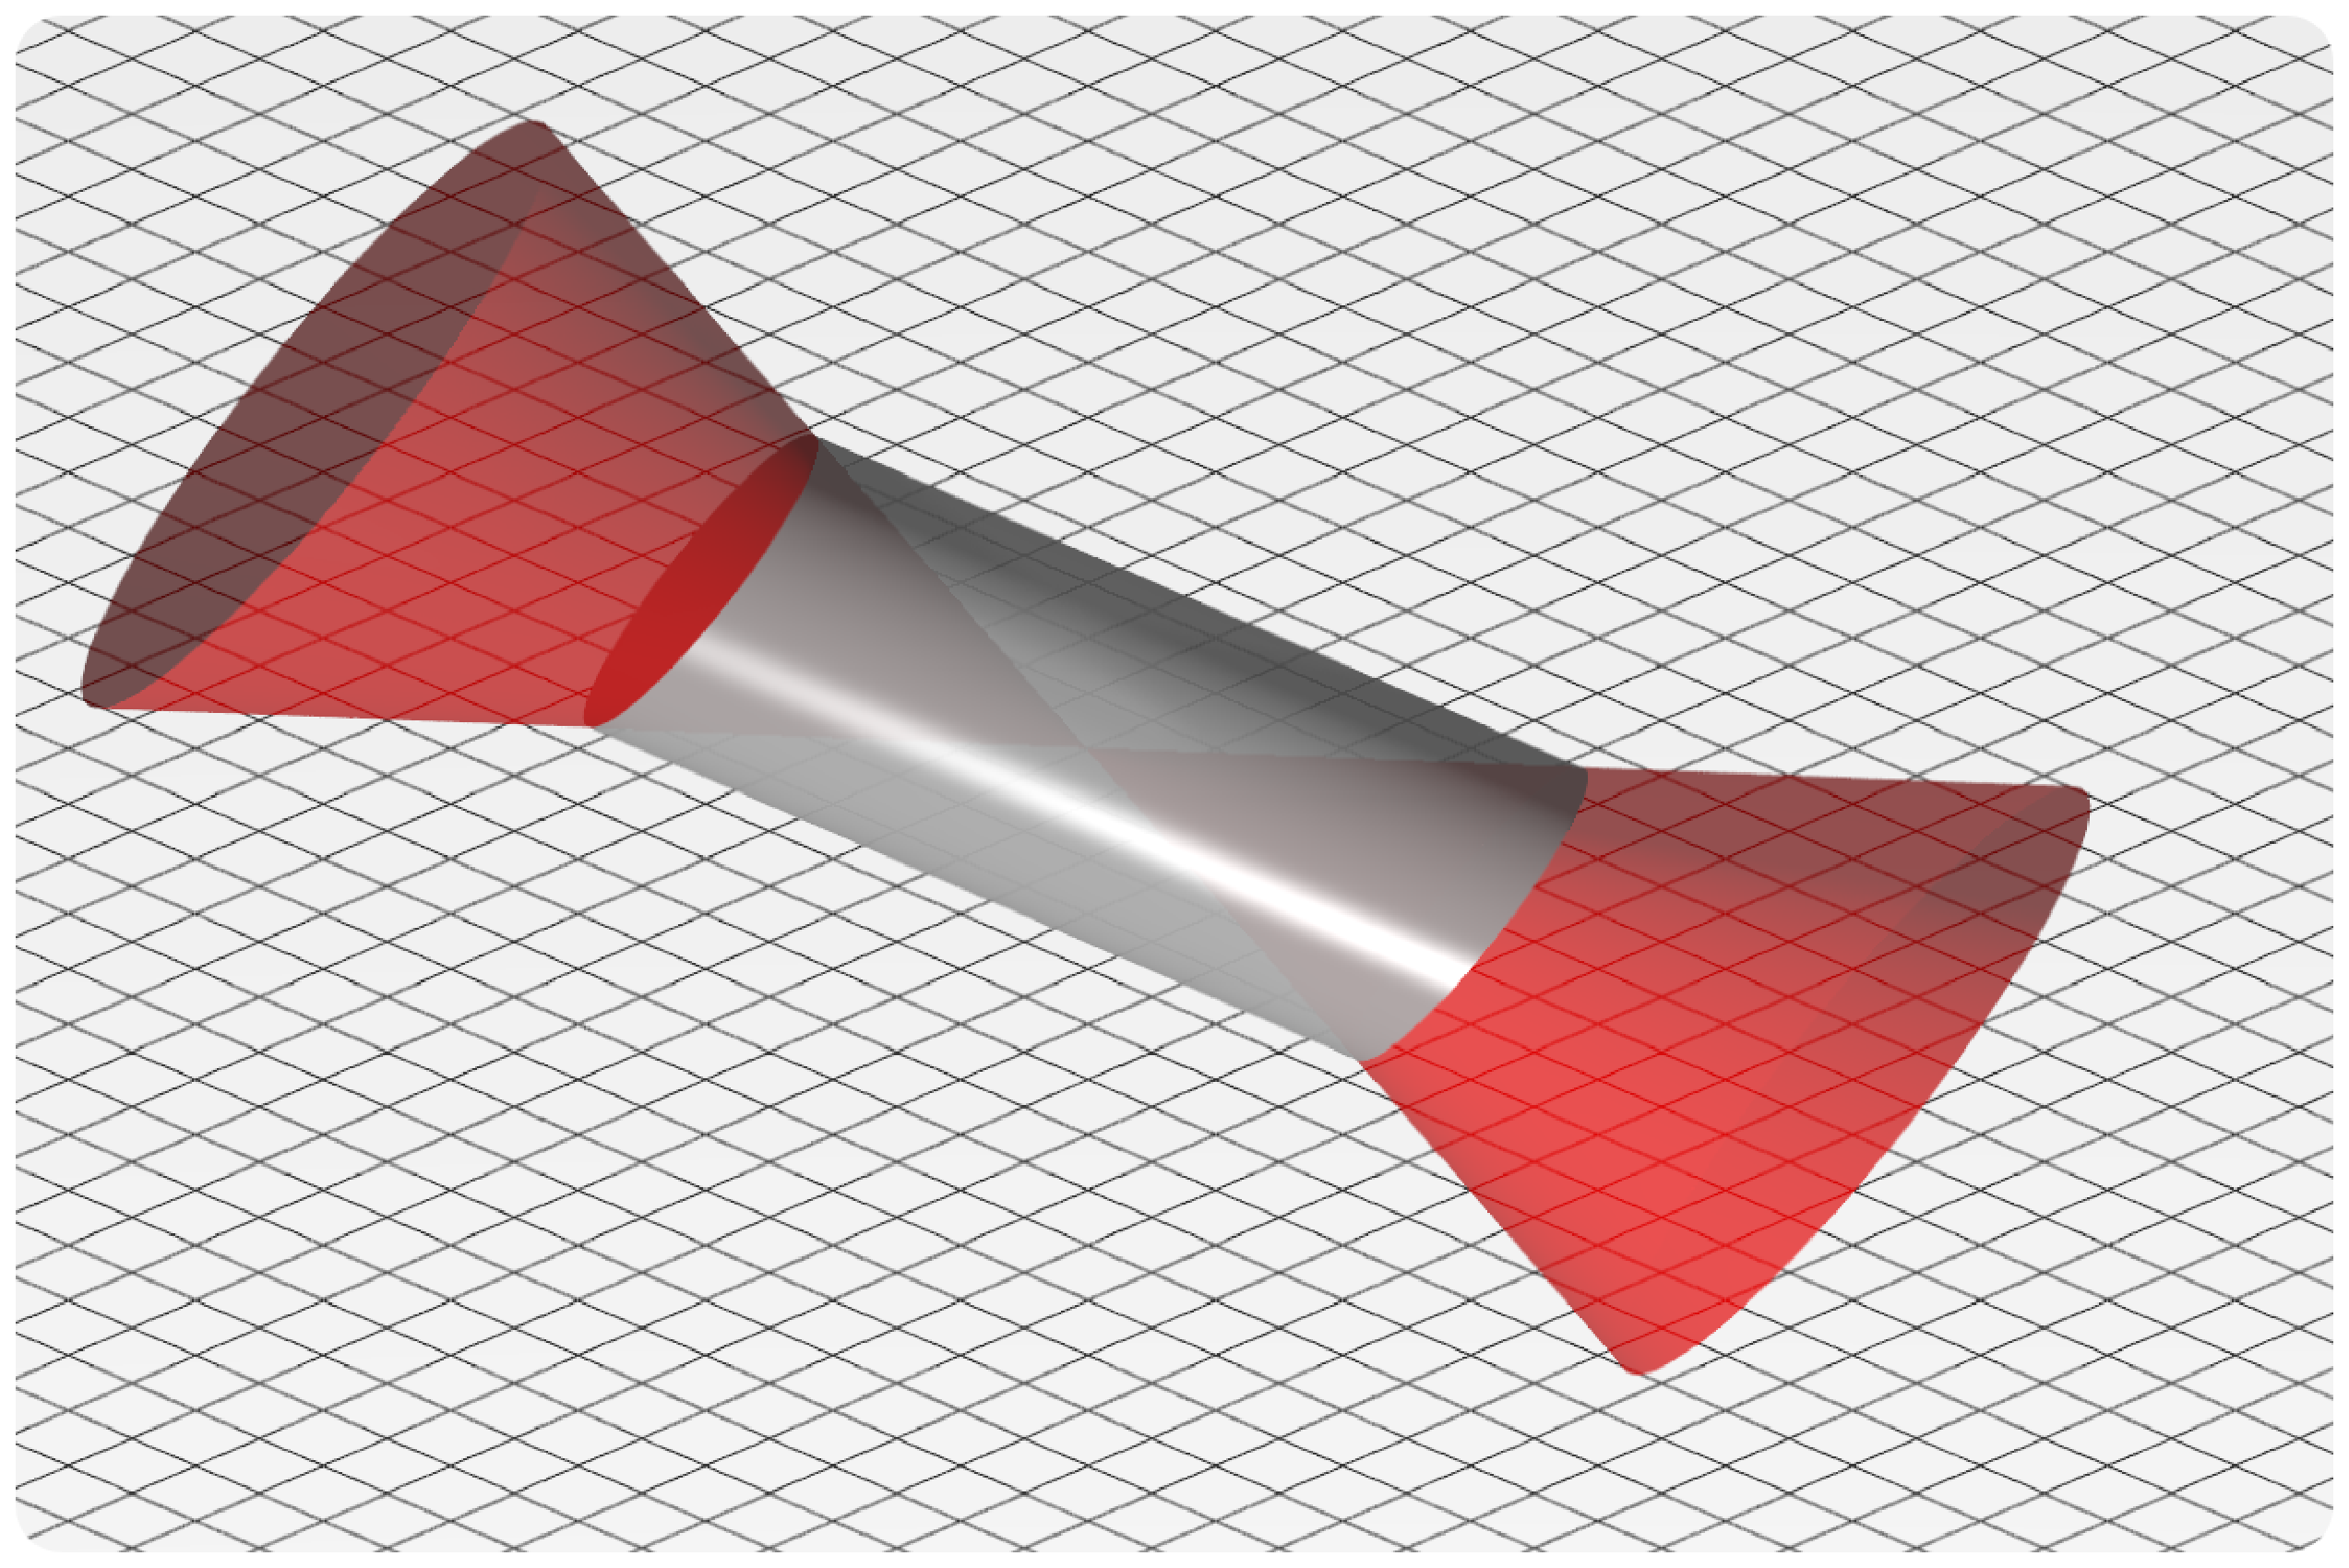
\includegraphics[width=\linewidth]{images/2cone.eps}
%\end{center}
%\caption{A double cone (red) representing the gradient discontinuities
%of a scalar field $f$.
%The field $f$ is the maximum of the distance to a line 
%and to a plane orthogonal to that line.
%The isosurfaces of $f$ are boundaries of cylinders.
%A sample isosurface is shown in green.
%The double cone separates $\Rthree$ into three regions.
%The field $f$ is continuous within each region.}
%\label{fig:double_cone}
%\end{figure}
\section{Determining Correct Gradients}
\label{sec:gradients}

We assume that the scalar values $s_v$ represent the values at the grid vertices $v$
of a continuous, piecewise smooth scalar field $f$. The difference between $s_v$ and $f(v)$ is the ``\textit{noise}'' in the data.

A scalar field $f :\Rthree \rightarrow \R$ is {\em piecewise smooth}
if $\Rthree$ can be partitioned into a finite set of piecewise smooth regions,
$A_1, A_2, \ldots, A_k$
such that $f$ has derivatives of all orders on each region $A_i$.
Because $f$ is only piecewise smooth,
the gradient field of $f$ may have discontinuities. Such discontinuities occur only on the boundaries, $\partial A_i$, 
of the $A_i$.

Figure~\ref{fig:double_cone} contains an example 
of a continuous piecewise smooth field,
consisting of three piecewise smooth regions
separated by two cones (a ``double cone'').
The isosurface for this field is the boundary of a cylinder.

The gradient at a point $p$ is the vector
$(\partial f/\partial x, \partial f/\partial y, \partial f/\partial z)$ at $p$.
Gradients are computed at some, but not all, of the grid vertices.
In particular, gradients are not computed at grid vertices \textit{on} 
or \textit{adjacent} to points where the scalar field is not smooth.

\subsection{Definitions}

We define the neighborhood of a grid vertex $v$.
Let set $N_1(v)$ be $v$ and the six grid vertices
which share a grid edge with $v$.
Recursively define set $N_k(v)$ as:
\begin{equation*}
N_k(v) = \{v': v' \in N_1(v'') \mbox{ for some } v'' \in N_{k-1}(v)\}.
\end{equation*}
We sometimes use $N(v)$ as an abbreviation for $N_1(v)$.

A {\em collinear sequence of adjacent grid vertices}
is a sequence $(v_1,v_2,\ldots,v_k)$ of distinct grid vertices
such that $v_i \in N(v_{i-1})$ for $i = 2,\ldots, k$
and all the $v_i$ are collinear.

An {\em interior grid vertex} of a region $A$
is a grid vertex $v$ such that $N(v)$ is a subset of $A$.
Set $\IV(A)$ is the set of all interior grid vertices of $A$.

%The {\em local feature size} of a point $p \in \XX$
%is the distance from $p$ to the medial axis of $\XX$.
%The local feature size is often used in analyzing 
%and proving the correctness of surface construction algorithms
%(e.g.~\cite{k-pgmls-08,dgqsww-fprss-12}.)


\subsection{Central Difference Formula}

To compute a gradient in a piecewise smooth scalar field,
we need all the scalar values used in the computation to be 
from a single smooth portion of the scalar field.
Thus, we want to use a small basis for our gradient computation
and not extend our gradient computation over many grid vertices.
We use the central difference formula
\begin{equation}
\partial f/\partial(x_d) \approx (f(x+u_d) - f(x-u_d))/(2|u_d|),
\label{eqn:cdiff}
\end{equation}
where $x$ is the location of a grid vertex and
$u_d$ is the vector to the adjacent vertex in direction $d$.
Figure~\ref{fig:grad-1} shows the result of computing
gradient using the central difference formula.

If spacing between grid vertices is the same in all directions,
then the grid can be rescaled so that $u_d$ is a unit vector 
in all directions.
However, CT scans often have non-uniform spacing,
with the $z$ or slice direction different from the $x$ and $y$ directions.
In that case, $u_x$ and $u_y$ will have different magnitudes from $u_z$.

Let $g_v$ be the gradient at a vertex $v$
and let $\tg_v$ be the gradient approximation produced 
by the central difference formula.
There are three types of errors in the approximation of $g_v$ by $\tg_v$.
First, there are errors caused by noise in the data,
i.e. the difference between the scalar value $s_v$ 
and it ``true'' value $f(v)$.
Second, there are errors caused by using the central difference formula
as an approximation to the gradient.
Such errors occur even if we used the exact values $f(v)$
and if the field was smooth everywhere.
Finally, if $v$ and one of its neighbors $v' \in N(v)$ 
lie in different smooth regions,
then there may be a discontinuity in the gradient along edge $(v,v')$.
This discontinuity will also contribute to errors in $\tg_v$. (Numerical error is a fourth contributor to errors in $\tg_v$,
but it is insignificant compared to the errors caused by noise in the data.)

Replacing the central difference formula by an equation 
which relies on more vertices will reduce the first two sources of error
but increase the effect of gradient discontinuities 
on the gradient approximation.
Anisotropic filtering can be used to decrease noise in the scalar data
without affecting the discontinuities,
but it will not reduce the error caused by gradient discontinuity.
Anisotropic filtering can also be used directly on the gradients.
Again, it will improve gradients in the smooth regions,
but it won't correct major errors caused by discontinuities.
(It might correct minor ones.)
\begin{figure}[t]
    \begin{center}
        \begin{tabular}{cc}
            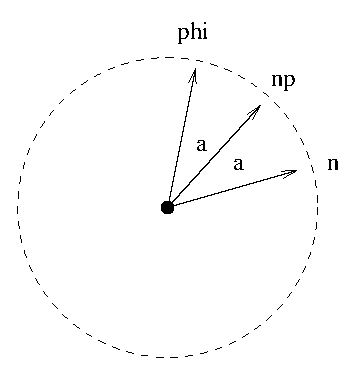
\includegraphics[width=0.25\linewidth]{images/predicted.eps} \qquad &
            \qquad
            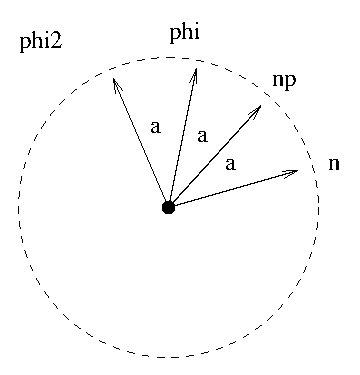
\includegraphics[width=0.25\linewidth]{images/predicted2.eps} \\
            (a) & (b)
        \end{tabular}
    \end{center}
    \caption{(a)~Vector $\phi(n,n')$ predicted by $n$ and $n'$.
        (b)~Vector $\phi_2(n,n')$ predicted by $n$ and $n'$.}
    \label{fig:predicted}
\end{figure}
%\begin{figure}[t]
%\begin{center}
%\begin{tabular}{cc}
%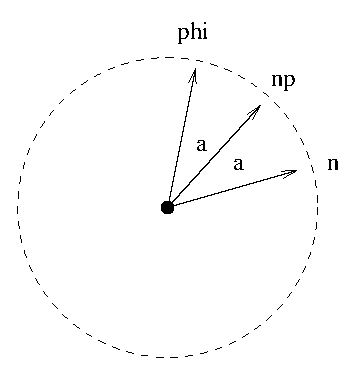
\includegraphics[width=1.4in]{images/predicted.eps} \qquad &
%\qquad
%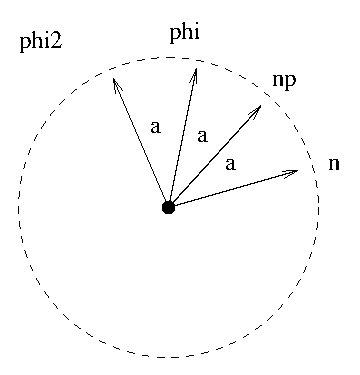
\includegraphics[width=1.4in]{images/predicted2.eps} \\
%(a) & (b)
%\end{tabular}
%\end{center}
%\caption{(a)~Vector $\phi(n,n')$ predicted by $n$ and $n'$.
%(b)~Vector $\phi_2(n,n')$ predicted by $n$ and $n'$.}
%\label{fig:predicted}
%\end{figure}

\subsection{Reliable Gradients}
\label{sec:reliable}

For each vertex $v$, let $\tn_v = \tg_v/|\tg_v|$ be the unit vector
in the direction of the central difference gradient $\tg_v$.
We can try to determine if the gradient direction $\tn_v$ at vertex $v$ 
is reliable by comparing it with the gradient directions $\tn_{v'}$
at all the neighboring vertices $v' \in N(v)$.
If $\angle(\tn_v,\tn_{v'})$ is less than some constant $\alpha$ 
for all vertices $v' \in N(v)$,
then we can mark the gradient at $v$ as reliable.

Determining reliable gradients from $\angle(\tn_v,\tn_{v'})$
will work for flat regions but will fail if
the scalar field has any significant curvature.
If $\alpha$ is set to a small value,
then the algorithm will fail to detect correct gradients
in curved regions.
On the other hand, if $\alpha$ is set to a large value,
then the algorithm will mark incorrect gradients as correct.
Instead of comparing $\tn_v$ to neighboring vertices,
we use pairs of vertices to predict the gradient direction at $v$
and compare $\tn_v$ to this predicted direction.

Let $n_v = g_v/|g_v|$ be the unit vector pointing in the direction
of the true gradient $g_v$.
Assume $(v,v',v'')$ is a collinear sequence of adjacent vertices.
Vectors $n_v$ and $n_{v'}$ lie in a plane $h$.
If the gradient changes at a constant rate along line segment $(v,v'')$,
then $n_{v''}$ also lies in plane $h$ and 
$\angle(n_{v'},n_{v''})$ equals $\angle(n_v,n_{v'})$.

Let $n$ and $n'$ be unit vectors in $\Rthree$\
lying plane $h$.
Let $\phi(n,n')$ be the unit vector in $h$ other than $n$
whose angle with $n'$ is $\angle(n,n')$.
We say that the $\phi(n,n')$ is the vector 
{\em predicted by} $n$ and $n'$.
(See Figure~\ref{fig:predicted}(a).)
More precisely, define $\Orth(n,n')$ as $ n - (n \cdot n') n'$,
the component of $n$ orthogonal to $n$.
Define $\phi(n,n')$ as:
\begin{align*}
\phi(n,n') & = n - 2 \times \Orth(n,n') 
             = n - 2(n - (n \cdot n')n')
             = 2(n \cdot n') n' - n.
\end{align*}

As defined above, unit vector $\tn_v = \tg_v/|\tg_v|$
points in the direction of the central difference gradient.
We determine reliable gradients 
by testing $\angle(\phi(\tn_{v''},\tn_{v'}),\tn_v)$ against a constant $\alpha$.
\begin{algorithm}[h]
\Input{Vertex $v$, Angle bound $\alpha$.}
\BlankLine
\ForEach{grid vertex $v' \in N(v)$}{
Let $v'' \in N(v')$ be the vertex such that
$(v,v',v'')$ is a collinear sequence of adjacent vertices\;
\lIf{($\angle(\phi(\tn_{v''},\tn_{v'}),\tn_v) > \alpha$)}{\Return(\false)}
}
\Return(\true)
\caption{}
\label{alg:curved}
\end{algorithm}

Assume $N_3(v)$ is a subset of a smooth region $A_i$ 
so that $v, v', v'' \in \IV(A_i)$ for all the neighbors $v'$ of $v$.
If all the second order partial derivatives of function $f$ in $A_i$
are constant,
then the gradients change at a constant rate
along any direction and $\phi(n_{v''},n_{v'})$ equals $n_v$.
Moreover, if all the second order partial derivatives are constant
and there is no noise ($s_v = f(v)$ for all $v$),
then the central difference gradient $\tg_v$ 
equals the exact gradient $g_v$ (up to numerical error.)
(See Proposition~\ref{prop:cdiff} in the appendix for a proof.)

In the more general case, 
the second order partial derivatives are not constant 
and there is noise in the data.
To analyze this case, define:
\begin{align*}
& \mu = \max\{ \angle(n_v,\tn_v) : v \in \IV(A_i) \mbox{ for some } A_i \}.\\
& \Lambda(n_v,n_{v'},n_{v''}) = \angle(\phi(n_v,n_{v'}),n_{v''}).\\
& \lambda = \max\{ \Lambda(n_v, n_{v'},n_{v''}) :
                  v,v',v'' \in A_i \mbox{ for some } A_i \}.
\end{align*}
Value $\mu$ is a bound on the angle 
between the approximate and exact gradient directions
in the smooth regions of the field.
$\Lambda(n_v,n_{v'},n_{v''})$ is the difference 
between the prediction $\phi(n_v,n_{v'})$ and $n_{v''}$.
This difference is caused by changes in the curvature of $f$.
Value $\lambda$ is a bound on this difference 
over vertices in the interiors of the $A_i$.
Note that Algorithm~\ref{alg:curved} 
computes $\Lambda(\tn_{v''},\tn_{v'},\tn_v)$,
not $\Lambda(n_v,n_{v'},n_{v''})$.

The following proposition bounds $\Lambda(\tn_v,\tn_{v'},\tn_{v''})$
and $\angle(n_{v''},\tn_{v''})$.
\begin{proposition}
Let $(v, v', v'')$ be a collinear sequence of adjacent vertices
contained in $A_i$ for some smooth region $A_i$.
\begin{enumerate}
\item If $v, v', v'' \in \IV(A_i)$, then\\
{\centering
$\Lambda(\tn_v, \tn_{v'}, \tn_{v''}) \le 
\Lambda(n_v, n_{v'}, n_{v''}) + 4 \mu \le \lambda + 4 \mu$.}
\item If $v, v' \in \IV(A_i)$, then
$\angle(n_{v''},\tn_{v''}) \le 
   \Lambda(\tn_v,\tn_{v'},\tn_{v''}) + 3 \mu + \lambda$.
\end{enumerate}
\label{prop:angle}
\end{proposition}

\begin{proof}[Outline of proof of \ref{prop:angle}.1:]
Perturbing $n_v$ by at most $\mu$,
changes $\phi(n_v,n_{v'})$ by at most $\mu$.
Since angles $\angle(n_v,\tn_v)$ and $\angle(n_{v''},\tn_{v''})$
are at most $\mu$,
angle $\angle(\phi(\tn_v,\tn_{v'}), \tn_{v''})$ is at most
$\angle(\phi(n_v,\tn_{v'}), n_{v''})+2 \mu$.

Perturbing $n_{v'}$ by at most $\mu$
changes $\phi(n_v,n_{v'})$ by at most $2\mu$.
Thus,
\begin{align*}
\Lambda(\tn_v, \tn_{v'}, \tn_{v''}) & 
= \angle(\phi(\tn_v,\tn_{v'}), \tn_{v''}) \\
& \le \angle(\phi(n_v,\tn_{v'}), n_{v''}) + 2 \mu\\
& \le \angle(\phi(n_v,n_{v'}), n_{v''}) + 2 \mu + 2 \mu\\
& = \Lambda(n_v,n_{v'},n_{v''}) + 4 \mu.
\end{align*}
\end{proof}

\begin{proof}[Outline of proof of \ref{prop:angle}.2:]
By the triangle inequality,
\begin{align*}
\angle(n_{v''},\tn_{v''}) & \le 
\angle(\phi(n_v,n_{v'}),n_{v''}) + \angle(\phi(n_v,n_{v'}),\tn_{v''}) \\
& \le \lambda + \angle(\phi(n_v,n_{v'}),\tn_{v''}).
\end{align*}
As discussed above, perturbing $n_v$ by at most $\mu$
changes $\phi(n_v,n_{v'})$ by at most $\mu$.
Perturbing $n_{v'}$ by at most $\mu$
changes $\phi(n_v,n_{v'}$ by at most $2\mu$.
Thus,
\begin{align*}
\angle(n_{v''},\tn_{v''}) 
& \le \lambda + \angle(\phi(n_v,n_{v'}),\tn_{v''}) \\
& \le \lambda + \angle(\phi(\tn_v, \tn_{v'}), \tn_{v''}) + 3\mu \\
& = \Lambda(\tn_v,\tn_{v'},\tn_{v''}) + \lambda + 3\mu.
\end{align*}
\end{proof}
More complete versions of these proofs are in the appendix.

Assume that parameter $\alpha$ in Algorithm~\ref{alg:curved} 
is at least $\lambda + 4 \mu$.
By the first inequality, 
if $N_3(v) \subseteq A_i$ for some $A_i$,
then $\Lambda(\tn_{v''}, \tn_{v'}, \tn_v) \le \lambda+4\mu \le \alpha$
for all neighbors $v'$ of $v$.
Thus Algorithm~\ref{alg:curved} returns true.

On the other hand, assume that Algorithm~\ref{alg:curved} returns true
and that $N_3(v)$ intersects at most two regions.
Let $A_i$ be the region containing $v$.
Under the assumption that the boundary between these two regions is planar,
some $v' \in N(v)$ is in $\IV(A_i)$.
If $(v,v',v'')$ is a collinear sequence of adjacent vertices,
then $v''$ is also in $\IV(A_i)$.
By the second inequality,
$\angle(n_v,\tn_v) \le \Lambda(\tn_{v''},\tn_{v'},\tn_v) + 3 \mu + \lambda
\le \alpha + 3 \mu + \lambda$.
Thus, if Algorithm~\ref{alg:curved} returns true,
then the angle between the approximate gradient direction $\tn_v$
and the true gradient direction $n_v$
is bounded by $\alpha + 3\mu + \lambda$.
 \begin{figure}
	\centering
    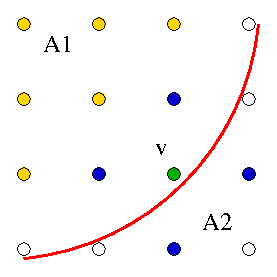
\includegraphics[width=0.5\linewidth]{images/curved_boundary.eps}
    \caption{Red curve is boundary separating regions $A_1$ and $A_2$.
        Green vertex $v$ is in $A_1$ but 
        no vertex of $N(v)$ lies in $\IV(A_1)$.
        Vertices in $N(v)$ are colored blue.
        Vertices in $\IV(A_1)$ are colored yellow.}
    \label{fig:curved_boundary}
    
 \end{figure}
    
%\begin{figure}
%	\centering
%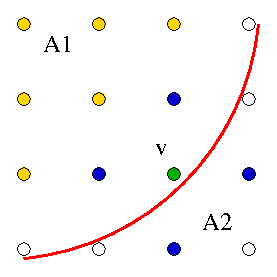
\includegraphics[width=0.25\linewidth]{images/curved_boundary.eps}
%	\caption{Red curve is boundary separating regions $A_1$ and $A_2$.
%           Green vertex $v$ is in $A_1$ but 
%           no vertex of $N(v)$ lies in $\IV(A_1)$.
%           Vertices in $N(v)$ are colored blue.
%           Vertices in $\IV(A_1)$ are colored yellow.}
%	\label{fig:curved_boundary}
%\end{figure}

So far we've made the assumption that the surface
between two smooth regions is planar.
If we drop that assumption, then it is no longer true
that for every vertex $v \in A_i$ some vertex in $N(v)$ is in $\IV(A_i)$.
For instance, in the 2D example in Figure~\ref{fig:curved_boundary},
no vertex in $N(v)$ lies in $\IV(A_1)$.
Without this property, we can no longer guarantee a bound
on $\angle(n_v, \tn_v)$ when Algorithm~\ref{alg:curved} returns true.

To handle curved boundaries of the $A_i$,
we must modify our algorithm to use vertices 
at edge distance 3 from $v$.
We define $\phi_k(n_v,n_{v'})$ as the normal direction 
predicted by $n_v$ and $n_{v'}$ at the vertex 
which is edge distance $k$ from $n_{v'}$.
\begin{align*}
\phi_0(n,n') & = n', \\
\phi_1(n,n') & = \phi(n,n') = 2 (n \cdot n') n' - n, \\
\phi_k(n,n') & = \phi(\phi_{k-2}(n,n'),\phi_{k-1}(n,n')), \\
\Lambda_k(n,n',n'') & = \angle(\phi_k(n,n'),n'').
\end{align*}

We replace $\phi$ in Algorithm~\ref{alg:curved} with $\phi_2$.
\begin{algorithm}[h]
\Input{Vertex $v$, Angle bound $\alpha$.}
\BlankLine
\ForEach{grid vertex $v' \in N(v)$}{
Let $v'',v''' \in N_3(v)$ be the vertices such that
$(v,v',v'',v''')$ is a collinear sequence of adjacent vertices\;
\lIf{($\angle(\phi(\tn_{v''},\tn_{v'}), \tn_v) > \alpha$)}{\Return(\false)}
\lIf{($\angle(\phi_2(\tn_{v'''},\tn_{v''}), \tn_v) > \alpha$)}
{\Return(\false)}
}
\Return(\true)
\caption{}
\label{alg:phi2}
\end{algorithm}

Let $A_i$ be the smooth region containing vertex $v$.
Let $\XX = \cup_{A_j} \partial A_j$ be the union of all the boundaries
of smooth regions $A_j$.
If there is a sufficiently large ball containing $v$
and not intersecting $\XX$, then $v'',v''' \in \IV(A_i)$
for some collinear sequence $(v,v',v'',v''')$.
\begin{proposition}
Let $\Gamma$ be a regular grid whose edges all have the same length $L$.
If some ball $\BB$ of radius $(5/2)\sqrt{3}L$ contains grid vertex $v \in A_i$
and does not intersect $\XX$,
then there is a collinear sequence $(v,v',v'',v''')$ 
of adjacent grid vertices 
such that $v'' \in \IV(A_i)$ and $v''' \in \IV(A_i)$.
\label{prop:IV}
\end{proposition}

To prove Proposition~\ref{prop:IV}, 
we show that there $\BB$ contains $N_v(v'')$ and $N_v(v''')$
for some collinear sequence $(v,v',v'',v''')$.
The proof is in the appendix.

The following proposition bounds $\Lambda_2(\tn_v,\tn_{v'},\tn_{v'''})$
and $\angle(n_{v'''},\tn_{v'''})$.
\begin{proposition}
Let $(v, v', v'',v''')$ be a collinear sequence of adjacent vertices
contained in $A_i$ for some smooth region $A_i$.
\begin{enumerate}
\item If $v, v', v'', v''' \in \IV(A_i)$, then\\
{\centering
$\Lambda_2(\tn_v, \tn_{v'}, \tn_{v'''}) \le 
\Lambda_2(n_v, n_{v'}, n_{v'''}) + 6 \mu \le 3\lambda + 6 \mu$.}
\item If $v, v' \in \IV(A_i)$, then\\
{\centering
$\angle(n_{v'''},\tn_{v'''}) 
   \le \Lambda(\tn_v,\tn_{v'},\tn_{v'''}) + 3\lambda+ 5 \mu$.}
\end{enumerate}
\label{prop:angle:b}
\end{proposition}
Proofs of these relationships are in the appendix.

As in the discussion, of Algorithm~\ref{alg:curved},
Property~\ref{prop:angle:b} can be used to show that 
if $N_4(v) \subset A_i$ for some $A_i$,
then Algorithm~\ref{alg:phi2} returns true.
On the other hand, assume Algorithm~\ref{alg:phi2} returns true.
By Proposition~\ref{prop:IV},
there is a collinear sequence of grid vertices $(v,v',v'',v''')$
such that $v'',v''' \in \IV(A_i)$.
By Proposition~\ref{prop:angle:b},
the angle between the approximate gradient direction $\tn_v$
and the true gradient direction $n_v$ is bounded by $\alpha + 3\lambda + 5 \mu$.

%The condition that a ball $\BB$ of radius $(5/2)\sqrt{3}$ 
%contains $v$ and does not intersect $\XX$
%can be formulated as a lower bound on the local feature size of $\XX$
%in the neighborhood of $v$.
%A lower bound on the local feature size of $\XX$ near $v$
%implies an upper bound on the curvature of $\XX$ near $v$.
%
%If the edge lengths of grid $\Gamma$ are not equal,
%then ball $\BB$ can be replaced by a suitable ellipsoid
%to give similar conditions for $v''$ and $v'''$ to be in $\IV(A_i)$.

\begin{algorithm}[h]
\NoLineNum{\DoesOrthMatchA{$v$, $\alpha_1$, $\alpha_2$}}
\lIf{($N^O(v) = \emptyset$)}{ \Return(\true)}
\ForEach{grid vertex $v' \in N^O(v)$}{
Let $v'',v''' \in N_3(v)$ be the vertices such that
$(v,v',v'',v''')$ is a collinear sequence of adjacent vertices
$\flagMatch \leftarrow \false$\;
\lIf{($\angle(\tn_v, \phi(\tn_{v''},\tn_{v'})) \le \alpha_2$) \KwAnd \\
     \hspace{1em} 
     ($\angle(\tn_v, \phi_2(\tn_{v'''},\tn_{v''})) \le \alpha_2$)}{
$\flagMatch \leftarrow \true$
}
\lIf{($\angle(\tn_v, \tn_{v'}) \le \alpha_1$) \KwAnd \\
    \hspace{1em} ($\angle(\tn_v, \tn_{v''}) \le \alpha_1$)}{
$\flagMatch \leftarrow \true$
}
\lIf{($\flagMatch = \false$)}{ \Return(\false) }
}
\Return(\true)
\caption{Algorithm \protect\DoesOrthMatchA.}
\label{alg:orthA}
\end{algorithm}
\begin{algorithm}[h]
\NoLineNum{\DoesOrthMatchB{$v$, $\alpha_1$}}
\ForEach{grid vertex $v' \in N^O(v)$}{
\If{($v \in N^O(v')$)}{
\lIf{($\angle(\tn_v,\tn_{v'}) \le \alpha_1$)}
{\Return(\true)}
}
}
\Return(\false)
\caption{Algorithm \protect\DoesOrthMatchB.}
\label{alg:orthB}
\end{algorithm}

\begin{algorithm}[h]
\NoLineNum{\FindReliable{$v$, $\alpha_1$, $\alpha_2$}}
\tcc{$\alpha_1$ and $\alpha_2$ are angle bounds}
\ForEach{grid vertex $v' \in N^T_v$}{
Let $v'',v''' \in N_3(v)$ be the vertices such that
$(v,v',v'',v''')$ is a collinear sequence of adjacent vertices\;
\lIf{($\angle(\tn_v, \phi(\tn_{v''},\tn_{v'})) > \alpha_2$)}{\Return(\false)}
\lIf{($\angle(\tn_v, \phi_2(\tn_{v'''},\tn_{v''})) > \alpha_2$)}
{\Return(\false)}
}
\lIf{\DoesOrthMatchA($v$, $\alpha_1$, $\alpha_2$)}
{ \Return(\true) }
\lElseIf{\DoesOrthMatchB($v$, $\alpha_1$)}
{ \Return(\true)}
\lElse{ \Return(\false)}
\caption{Algorithm \protect\FindReliable}
\label{alg:phi3}
\end{algorithm}



\subsection{CT Data}

Algorithm~\ref{alg:phi2} has two problems when applied to CT data.
First, 
in CT data scalar values near gradient discontinuities
are very unreliable.
At such vertices, the angle between the true gradient $n_v$
and the estimated gradient direction $\tn_v$ is also very unreliable.
Thus, we cannot assume that angle is bounded by a constant $\mu$
on vertices near gradient discontinuities.
Second, gradient magnitudes drop off quickly away from the surface boundaries
and gradient directions are quickly meaningless.
This is particularly true if the gradient direction is the z-direction
and the CT data is reconstructed in planar x-y slices.
We address each of these problems.

The first problem with CT data is that scalar values near gradient
discontinuities are very unreliable.
At such vertices,
the angle between $n_v$ and $\tn_v$ can be much greater 
than in the rest of the data set.
Unfortunately, gradients at vertices near gradient discontinuities 
are exactly the gradients which we need to generate sharp features.

Gradients generated from scalar data rely upon the accuracy
of the scalar data.
CT scanners do not measure scalar values directly at each grid vertex.
Instead, they measure the intensity of rays passing 
through the scanned object.
The resulting measurements are called projection data.
The projection data is transformed into scalar data
by using a Radon or similar transformation
of by solving a large set of linear equations.
The resolution of the scalar data is usually set to equal
the resolution of the projection data.

The process of determining scalar values at grid vertices
is provably reliable in regions where field gradients 
vary slowly and continuously.
However, it is highly unreliable near discontinuities 
in the field gradients.
The result is that scalar values at grid vertices
adjacent to gradient discontinuities are highly unreliable
and the angle between the true gradient and the estimated gradient
can be much larger than in the rest of the data.

Fortunately, the scalar errors drop off quickly away 
from the gradient discontinuities.
We found that scalar values at a grid vertex $v$ was reliable
within an acceptable tolerance as long as no edge incident on $v$
intersected a gradient discontinuity.
Equivalently, the scalar value at $v \in A_i$ was reliable
as long as $N(v)$ was a subset of $A_i$.
Under this assumption,
if $N_2(v)$ is contained in some smooth region $A_i$,
then the scalar values at vertices in $N(v)$ are close to their true values.
This implies that the angle between $n_v$ and $\tn_v$ is small.

Let $A_i$ be the smooth region containing grid vertex $v$.
Assume that the boundary of $A_i$ is flat around $v$.
We can no longer assume that the angle between $n_{v'}$ and $\tn_{v'}$
is small for some $v' \in N(v)$.
However, there is a collinear sequence $(v,v',v'',v''')$ 
of adjacent vertices such that $N_2(v'')$ and $N_2(v''')$ 
are in $A_i$.
Thus, $\tn_{v''}$ and $\tn_{v'''}$ are good estimates
of $n_{v''}$ and $n_{v'''}$, respectively.
By comparing $\tn_v$ with the direction $\phi_2(\tn_{v'''},\tn_{v''})$
predicted by $\tn_{v'''}$ and $\tn_{v''}$,
we can determine if $\tn_v$ is a reliable gradient.
Note that this exactly what Algorithm~\ref{alg:phi2} does.

The argument above assumes the boundary of $A_i$ is flat around $v$.
Without this assumption, we can no longer conclude that $N_2(v'')$
and $N_2(v''')$ are in $A_i$ for some collinear sequence $(v,v',v'',v''')$.

Assume that all grid edges have the same length $L$.
Replace the assumption that a scalar value at $v \in A_i$ is reliable
if $N(v) \subseteq A_i$
by the assumption that a scalar value at $v$ is reliable
if a ball $\BB_{0.5L}(v)$ of radius $0.5L$ around $v$ 
is contained in $A_i$.
Under this assumption,
if $\BB_{1.5L}(v)$ is contained in some smooth region $A_i$,
then the scalar values at the vertices $N(v)$ 
are all close to their true values.
This implies that the angle between $n_v$ and $\tn_v$ is small.

If $\BB'$ is a sufficiently large ball containing $v$ and $A_i$
contains $\BB'$,
then there is a collinear sequence $(v,v',v'',v''')$ 
of adjacent grid vertices 
such that $A_i$ contains $\BB_{1.5}(v'')$ and $\BB_{1.5}(v''')$.
Thus, $\tn_{v''}$ and $\tn_{v'''}$ are reliable gradients.
Algorithm~\ref{alg:phi2} determines if $\tn_v$ is reliable
from $\tn_{v''}$ and $\tn_{v'''}$.

The second problem with CT data is that gradient magnitudes 
drop off quickly away from the surface boundaries.
To address this problem,
we divide the vertex neighbors of $v$ into two sets.
Define the the tangent neighbor set and
the orthogonal neighbor set of $v$ as:
\begin{align*}
N^T(v) & = \{ v' \in N(v) : 
  20^\circ \le \angle(\tn_v,(v'-v)) \le 160^\circ. \} \\
N^O(v) & = N(v) - N^T_v \\
       & = \{ v' \in N(v) : \angle(\tn_v,(v'-v)) < 20^\circ \mbox{ or } \\
       & \qquad \qquad \angle(\tn_v,(v-v')) < 20^\circ. \}
\end{align*}
$(v'-v)$ is the vector from $v$ to $v'$.
The orthogonal neighbor set may be empty.

Assuming that $\tn_v$ is relatively close to $n_v$,
vertices in $N^T(v)$ are near the tangent plane at $v$
and close to the isosurface through $v$.
We handle gradient directions at those vertices as in Algorithm~\ref{alg:phi2}.
Vertices in $N^O(v)$ are (relatively) far from the tangent plane
and from the isosurface through $v$.
Fortunately, the gradient directions at the vertices in $N^O(v)$
are much more reliable than the gradient directions at vertices in $N^T(v)$.
Thus, we can use gradients at vertices in $N^O(v)$ 
to determine whether gradient $\tn_v$ is reliable.
We reduce the number of nearby vertices whose gradient directions
must match $\tn_v$ in three ways.

First, we note that there is little curvature along the gradient direction
in the scalar field represented by a CT scan.
Thus, in addition to the comparison 
of $\tn_v$ and $\phi_2(\tn_{v'''},\tn_{v''})$,
we can simply compare $\tn_v$ and $\tn_{v''}$.
If angle $\angle(\tn_v,\tn_{v''})$ is below some threshold $\alpha_1$,
then $\tn_{v''}$ can be a guarantor of the reliability of $\tn_v$.
(See Algorithm~\ref{alg:orthA}.)

Second, instead of comparing $\tn_v$ and $\tn_{v''}$,
we compare $\tn_v$ to its immediate neighbor $\tn_{v'} \in N(v)$
(Algorithm~\ref{alg:orthB}.)
We still compare $\tn_v$ with vertices at edge distance 3
in the tangent directions.
If some sufficiently large ball contains $v \in A_i$
and does not intersect $\XX = \cup_{A_j} \partial A_j$,
then either there is a $v' \in N^T(v)$ and collinear sequence $(v,v',v'',v''')$
where $v'',v''' \in \IV(A_i)$
or there is a $v' \in N^O(v)$ such that $v' \in \IV(A_i)$.

Third, in Algorithm~\ref{alg:orthB}
we replace the requirement that gradient directions 
of both vertices in $N^O(v)$ ``match'' $\tn_v$
by a requirement that the gradient direction of one vertex
in $N^O(v)$ matches $\tn_v$.
Let $N^O(v) = \{v'_1, v'_2\}$.
We require that either the $\angle(\tn_v, \tn_{v'_1})$ 
or that $\angle(\tn_v, \tn_{v'_2})$  is small.
To make sure that we are only applying the single check
to gradients which truly point along an axis,
we require also that $\tn_{v'_1}$ or $\tn_{v'_2}$
be close to the axis direction.

Algorithm~\ref{alg:orthA} contains the check
in both orthogonal directions.
Algorithm~\ref{alg:orthB} contains the additional check 
in one orthogonal direction.
Because of the check $v \in N^O(v')$ in line 2 of Algorithm~\ref{alg:orthB},
there are cases where Algorithm~\ref{alg:orthA} may return true
while Algorithm~\ref{alg:orthB} returns false.
Algorithm~\ref{alg:phi3} is the full algorithm.

Algorithm~\ref{alg:phi3} loosens the conditions 
under which a gradient is identified as reliable.
By Proposition~\ref{prop:angle:b},
if $N_4(v) \subset A_i$ for some $A_i$,
then Algorithm~\ref{alg:phi3} returns true.
What about the converse, i.e. if Algorithm~\ref{alg:phi3} returns true?

We can show that for each $v \in A_i$,
there is either a collinear sequence of grid vertices $(v,v',v'',v''')$
such that $v' \in N^T(v)$ and $v'',v''' \in \IV(A_i)$
or there is a vertex $v' \in N^O(v)$ such that $v' \in \IV(A_i)$.
(See Proposition~\ref{prop:IV:b} in the appendix.)
In the first case,
the angle between the approximate gradient direction $\tn_v$
and the true gradient direction $n_v$ is bounded 
by $\alpha_2 + 3\lambda + 5 \mu$.
In the second case,
the angle between $\tn_v$ and $n_v$ is bounded by
$\angle(\tn_v,\tn_{v'}) + \kappa + \mu$
where $\kappa$ is a bound on curvature.
(See Prop~\ref{prop:kappa} in the appendix.)
If $\angle(\tn_v,\tn_{v'}) \le \alpha_1$,
then $\angle(\tn_v,n_v) \le \alpha + \kappa + \mu$.
However, Algorithm \DoesOrthMatchB (Algorithm~\ref{alg:orthB}),
only guarantees that $\angle(\tn_v, \tn_w) \le \alpha_1$
for one vertex $w \in N^O(v)$.
What if $w$ is not the vertex of $N^O(v)$ which is in $\IV(A_i)$?

We think that if $\angle(\tn_v,\tn_w) \le \alpha_1$ for one $w \in N^O(v)$
and $\angle(\tn_v,\phi_2(\tn_{w'''},\tn_{w''})) \le \alpha_2$
for all collinear sequences $(v,w',w'',w''')$ where $w' \in N^T(v)$,
then $\angle(\tn_v, n_v)$ is small.
However, we don't yet have a proof.


\begin{algorithm}[h]
\NoLineNum{\ExtendReliable{$\alpha_2$, $\numIter$}}
\For{$k \leftarrow 1$ \KwTo $\numIter$}{
$S \leftarrow \emptyset$\;
\ForEach{vertex $v$}{
\ForEach{vertex $v' \in N^T(v)$}{
Let $v'',v''' \in N_3(v)$ be the vertices such that
$(v,v',v'',v''')$ is a collinear sequence of adjacent vertices\;
\If{($v'$, $v''$ and $v'''$ are marked reliable)}{
\If {($\angle(\tn_v,\phi(\tn_{v''},\tn_{v'})) < \alpha_2$) \KwAnd
     ($\angle(\tn_v,\phi_2(\tn_{v'''},\tn_{v''})) < \alpha_2$)}
{ $S \leftarrow S \cup \{v\}$\; }
}
}
}
Mark each vertex $v \in S$ as reliable\;
}
\caption{Algorithm \protect\ExtendReliable}
\label{alg:extend}
\end{algorithm}

\subsection{Extending Reliable Gradients}
\label{sec:extendGrad}
Once we've identified reliable gradients by Algorithm~\ref{alg:phi3},
we can use those reliable gradients to identify vertex neighbors
with reliable gradients.
By Proposition~\ref{prop:angle:b},
if $v''$ and $v'''$ are reliable and 
$\angle(\phi_2(\tn_{v'''},\tn_{v''}), \tn_v)$ is small,
then $\angle(\tn_v, n_v)$ is small.
This is particularly helpful near gradient discontinuities,
where Algorithm~\ref{alg:phi3} will fail to identify correct gradients
as reliable because some of their neighbors are incorrect.

Pseudo code for Algorithm~\ExtendReliable is given 
in Algorithm~\ref{alg:extend}.
Because the initial set of reliable gradients is computed
If the initial set of reliable gradients is computed using $(v,v',v'',v''')$,
the value of $\numIter$ is set to 2.

\begin{algorithm}[h]
\NoLineNum{\ReliGrad{$\alpha_1$, $\alpha_2$, $\numIter$}}
\lForEach{grid vertex $v$}{
\FindReliable{$v$,$\alpha_1$,$\alpha_2$}
}
\ExtendReliable{$\alpha_2$, $\numIter$}
\BlankLine
\caption{Algorithm \protect\ReliGrad}
\label{alg:religrad}
\end{algorithm}

\subsection{Algorithm \protect\ReliGrad}
\label{sec:ReliGrad}

Our final algorithm, named \ReliGrad, applies Algorithm~\FindReliable
to each vertex and then calls \ExtendReliable.
Pseudo code is in Algorithm~\ref{alg:religrad}.


% Gradient selection

\section{Selecting Gradients}
\label{sec:grad_select}

Once we have identified reliable gradients,
we use those gradients to compute planes tangent to the isosurface
in the neighborhood of each cube $\cb$.
Algorithm~MergeSharp in~\cite{bw-cisec-13}
uses gradients at the vertices of $\cb$ and cubes adjacent to $\cb$.
Unfortunately, if cube $\cb$ intersects a gradient discontinuity,
this neighborhood may contain no or few reliable gradients.
We can only guarantee that a vertex $v \in A_i$ will pass the angle test
in Step~3 of \FindReliable (Algorithm~\ref{alg:phi3}),
if $N(v''') \subseteq A_i$ for each collinear sequence $(v,v',v'',v''')$
where $v' \in N^T(v)$.
Thus, vertex $v$ should be at least four edges from the boundary of $A_i$
in each of the tangent directions.

Algorithm \ExtendReliable (Algorithm~\ref{alg:extend}) increases
the number of reliable gradients close to the gradient discontinuities.
On the other hand, if a cube contains an isosurface corner,
then the distance to reliable gradients may be even larger than four.
Thus, we look for reliable gradients in a $9 \times 9 \times 9$ region
around cube $\cb$ or distance 4 from the vertices of $\cb$.

We are interested only in selecting gradients 
which determine isosurface tangent planes near $\cb$.
We use three tests on vertices in the $9 \times 9 \times 9$ region
to select such gradients.
First, we are only interested in vertices which are near the isosurface.
Thus, we only choose vertices from edges
where one endpoint has scalar value below
the isovalue and one endpoint has scalar value at or above the isovalue.
Second, we are only interested in vertices whose gradients generate planes
which are close to $\cb$.
Let $h_v$ be the tangent plane generated by the gradient at vertex $v$.
We construct a cube $\cb'$ of size $1.5 \times 1.5 \times 1.5$ centered at $\cb$
and only choose a vertex $v$ if the plane $h_v$ intersects $\cb'$.
(We use a cube $\cb'$ which is slightly larger than $\cb$ 
because noise and approximation errors can cause a tangent plane $h_v$ 
to slightly miss $\cb$.)

Finally, we only want to choose a vertex which is far from $\cb$
if a closer vertex is not chosen.
Let $Q$ be the set of vertices which do NOT have reliable gradients
and are in the $9 \times 9 \times 9$ subgrid centered at $\cb$.
Let $Q_\cb$ be the vertices of $\cb$.
Let $G_\cb$ be the graph whose vertices are $Q \cup Q_\cb$
and whose edges are $(u,v)$ where $(u,v)$ is a grid edge.
We find the connected component $G'$ of $G_\cb$ containing $Q_\cb$.
A grid vertex $u \not\in V(G')$ is on the boundary of $G'$
if $(u,v)$ is a grid edge and $v$ is in $V(G')$.
We only a choose a vertex if it is in $Q_\cb$
or if it is on the boundary of $G'$.

Applying the three tests gives a set of vertices 
and their reliable gradients around cube $\cb$.
As described in the next section,
we use these gradients to determine the locations 
of isosurface vertices on sharp features.



% \begin{wrapfigure}{r}{0.5\linewidth}
%\centering
%\includegraphics[width=0.6\linewidth]{images/mergesharp.3.eps}

%\caption{Isosurface mesh constructed by {\sc MergeSharp}.
%    Red isosurface vertices are the sparse selected edge vertices. The inset shows all the edge vertices generated in green, the larger blue cube shows the neighborhood around the smaller blue internal cube, all the green vertices in this larger neighborhood are merged to the isosurface vertex generated by the interior blue cube.}

%\label{fig:cubeB}    \end{wrapfigure}

%\begin{figure}
%\centering
%\includegraphics[width=0.6\linewidth]{images/mergesharp.3.eps}
%
%\caption{Isosurface mesh constructed by {\sc MergeSharp}.
%Red isosurface vertices are the sparse selected edge vertices. The inset shows all the edge vertices generated in green, the larger blue cube shows the neighborhood around the smaller blue internal cube, all the green vertices in this larger neighborhood are merged to the isosurface vertex generated by the interior blue cube.}
%
%\label{fig:cubeB}
%\end{figure}

\section{Computing Points on Sharp Features}
\label{sec:computeSharpPoints}

Once we have reliable gradients,
we can use those gradients to compute the location of isosurface vertices 
on sharp edges and corners.
The gradients can also be used to compute the location 
of isosurface vertices on smooth regions of the isosurface.
The algorithm for computing isosurface vertices from gradients
is given in~\cite{bw-cisec-13}.
It is a modification of Lindstrom's algorithm in~\cite{l-oslpm-00},
with surface normals replaced by gradients.

Let $g_i$ and $s_i$ be the gradient and scalar value, respectively,
at point $p_i$.
Let $\sigma$ be the isovalue.
The set $h_i = \{x : g_i \cdot (x-p_i) + s_i = \sigma \}$ is a plane in 3D.
Equivalently, plane $h_i$ is
$\{x : g_i \cdot x = \sigma - (g_i \cdot p_i + s_i) \}$.

Given a set $\{(p_i,g_i,s_i)\}$ of $k$ points and their associated
gradients and scalar values,
define a matrix $M$ whose $i$'th row is $g_i/|g_i|$
and a column vector $b$ whose $i$'th element is 
$(\sigma - (g_i \cdot p_i + s_i))/|g_i|$.
(We divide by $|g_i|$ so that all normal directions have equal weight.)
This gives a set of $k$ equations $Mx = b$
where $M$ is a $k\times3$ matrix and $x$ and $b$ are column vectors
of length $k$.
In general, this system is over-determined so we wish to find
the least squares solution.

We use the singular valued decomposition (SVD) of $M^T M$
to find an approximate solution $x^*$ to $M x = b$.
We use the number of large singular values of $A$
to determine whether $x^*$ is on a sharp corner,
a sharp edge or a smooth region on the surface.
Details are in Appendix~\ref{appendix:Lindstrom}.

% Selecting sharp vertices

\section{Sparsifying Isosurface Vertices}
\label{sec:select_sharp}

The algorithm in the previous section produces one isosurface vertex
for each grid cube intersected by the isosurface.
Points on sharp edges and corners are identified 
as such by the algorithm.
However, isosurface vertices on sharp features
may lie very close together.
If those vertices are used for mesh generation
or are joined together to form sharp curves,
they need to sparsified so there is spacing between them.
Fortunately, the grid structure makes this easy.
We use a procedure from~\cite{bw-cisec-13}
to sparsify the set of isosurface vertices on sharp features.

Let $S$ be the list of isosurface vertices on sharp features
sorted by increasing distance from the grid cube centers.
Select the first vertex $v$ in $S$.
Let $\cb$ be the cube containing $v$.
Delete any vertices of $S$ which lie in $\cb$ 
or in any of the 26 grid cubes which share a vertex with $\cb$.
Repeat until $S$ contains no more vertices.
If all grid edges have length $L$,
then the resulting isosurface vertices are never closer
than distance $L$.
Figure~\subref*{fig:setA.crop1.mesh.2} shows the original sharp edge vertices and figure~\subref*{fig:setA.crop1.mesh.3} shows the sparse set for an edge in a real CT dataset.





\section{Experimental Results}
\subsection{Synthetic datasets}
%\begin{figure*}[htb]
%    \centering
%    \subfloat[ TwoCube]{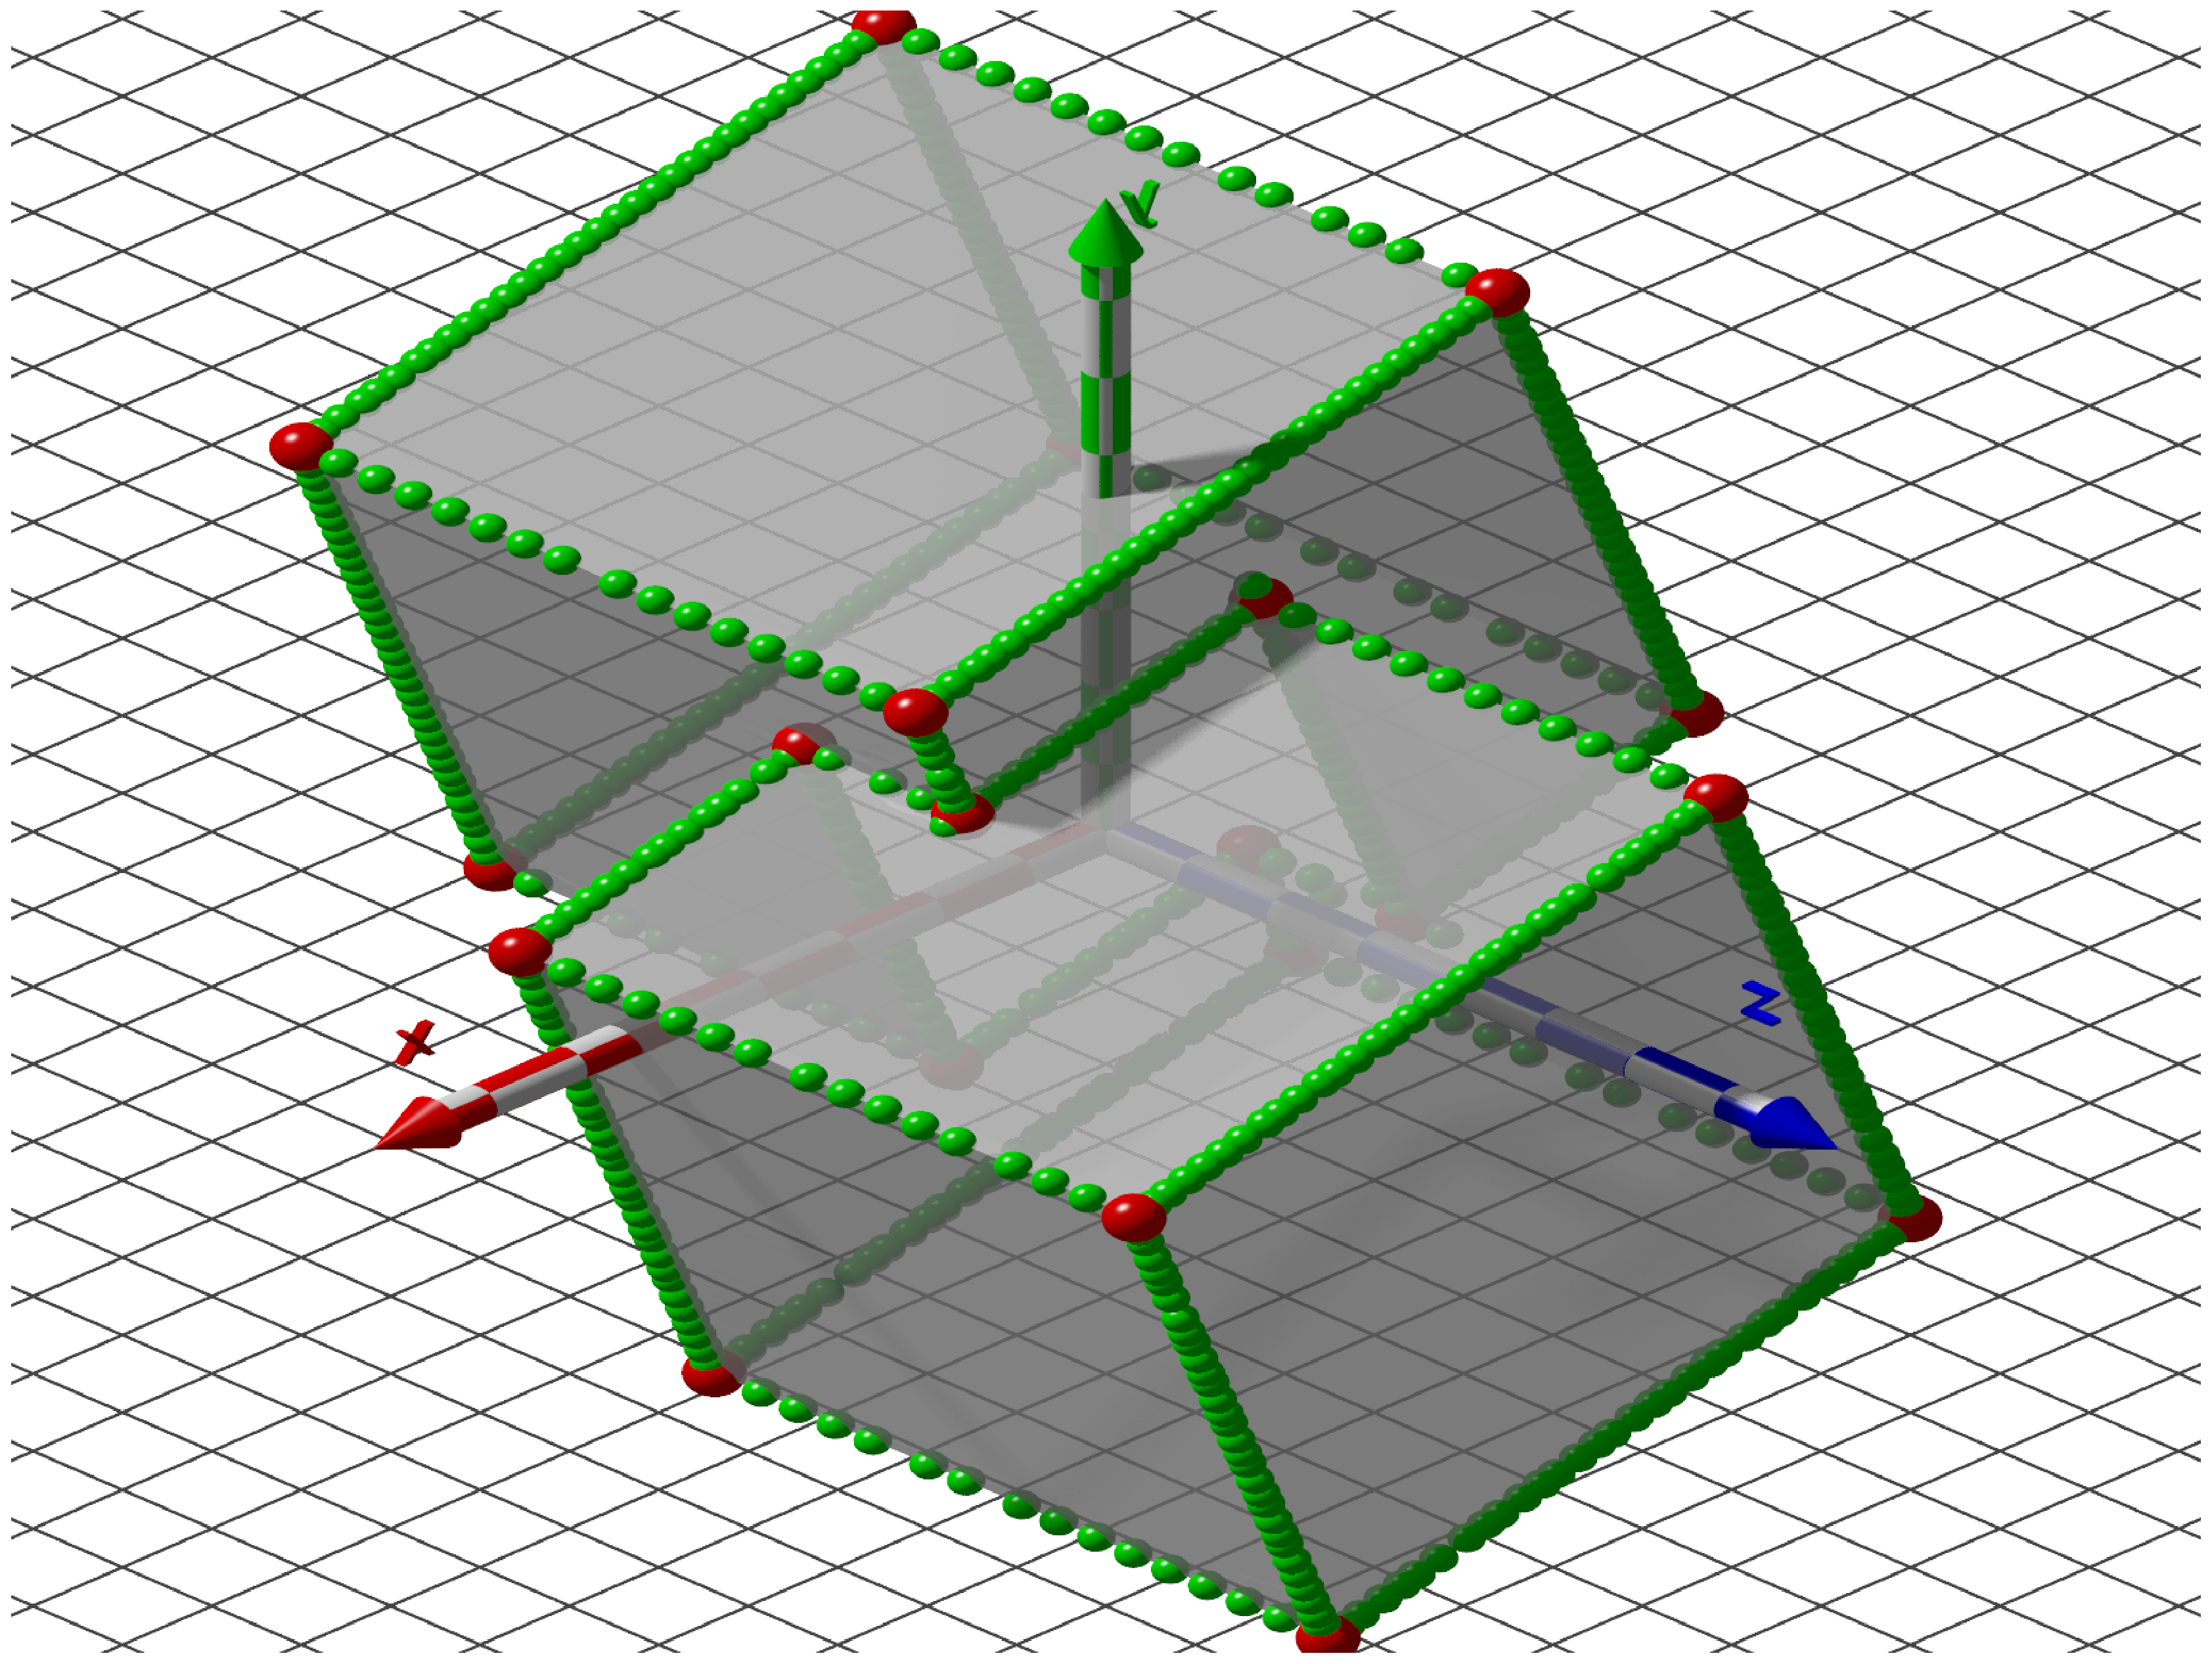
\includegraphics[width=0.2\linewidth]{images/twoCube.B.eps}\label{fig:TwoCube}}
%    \subfloat[Flange]{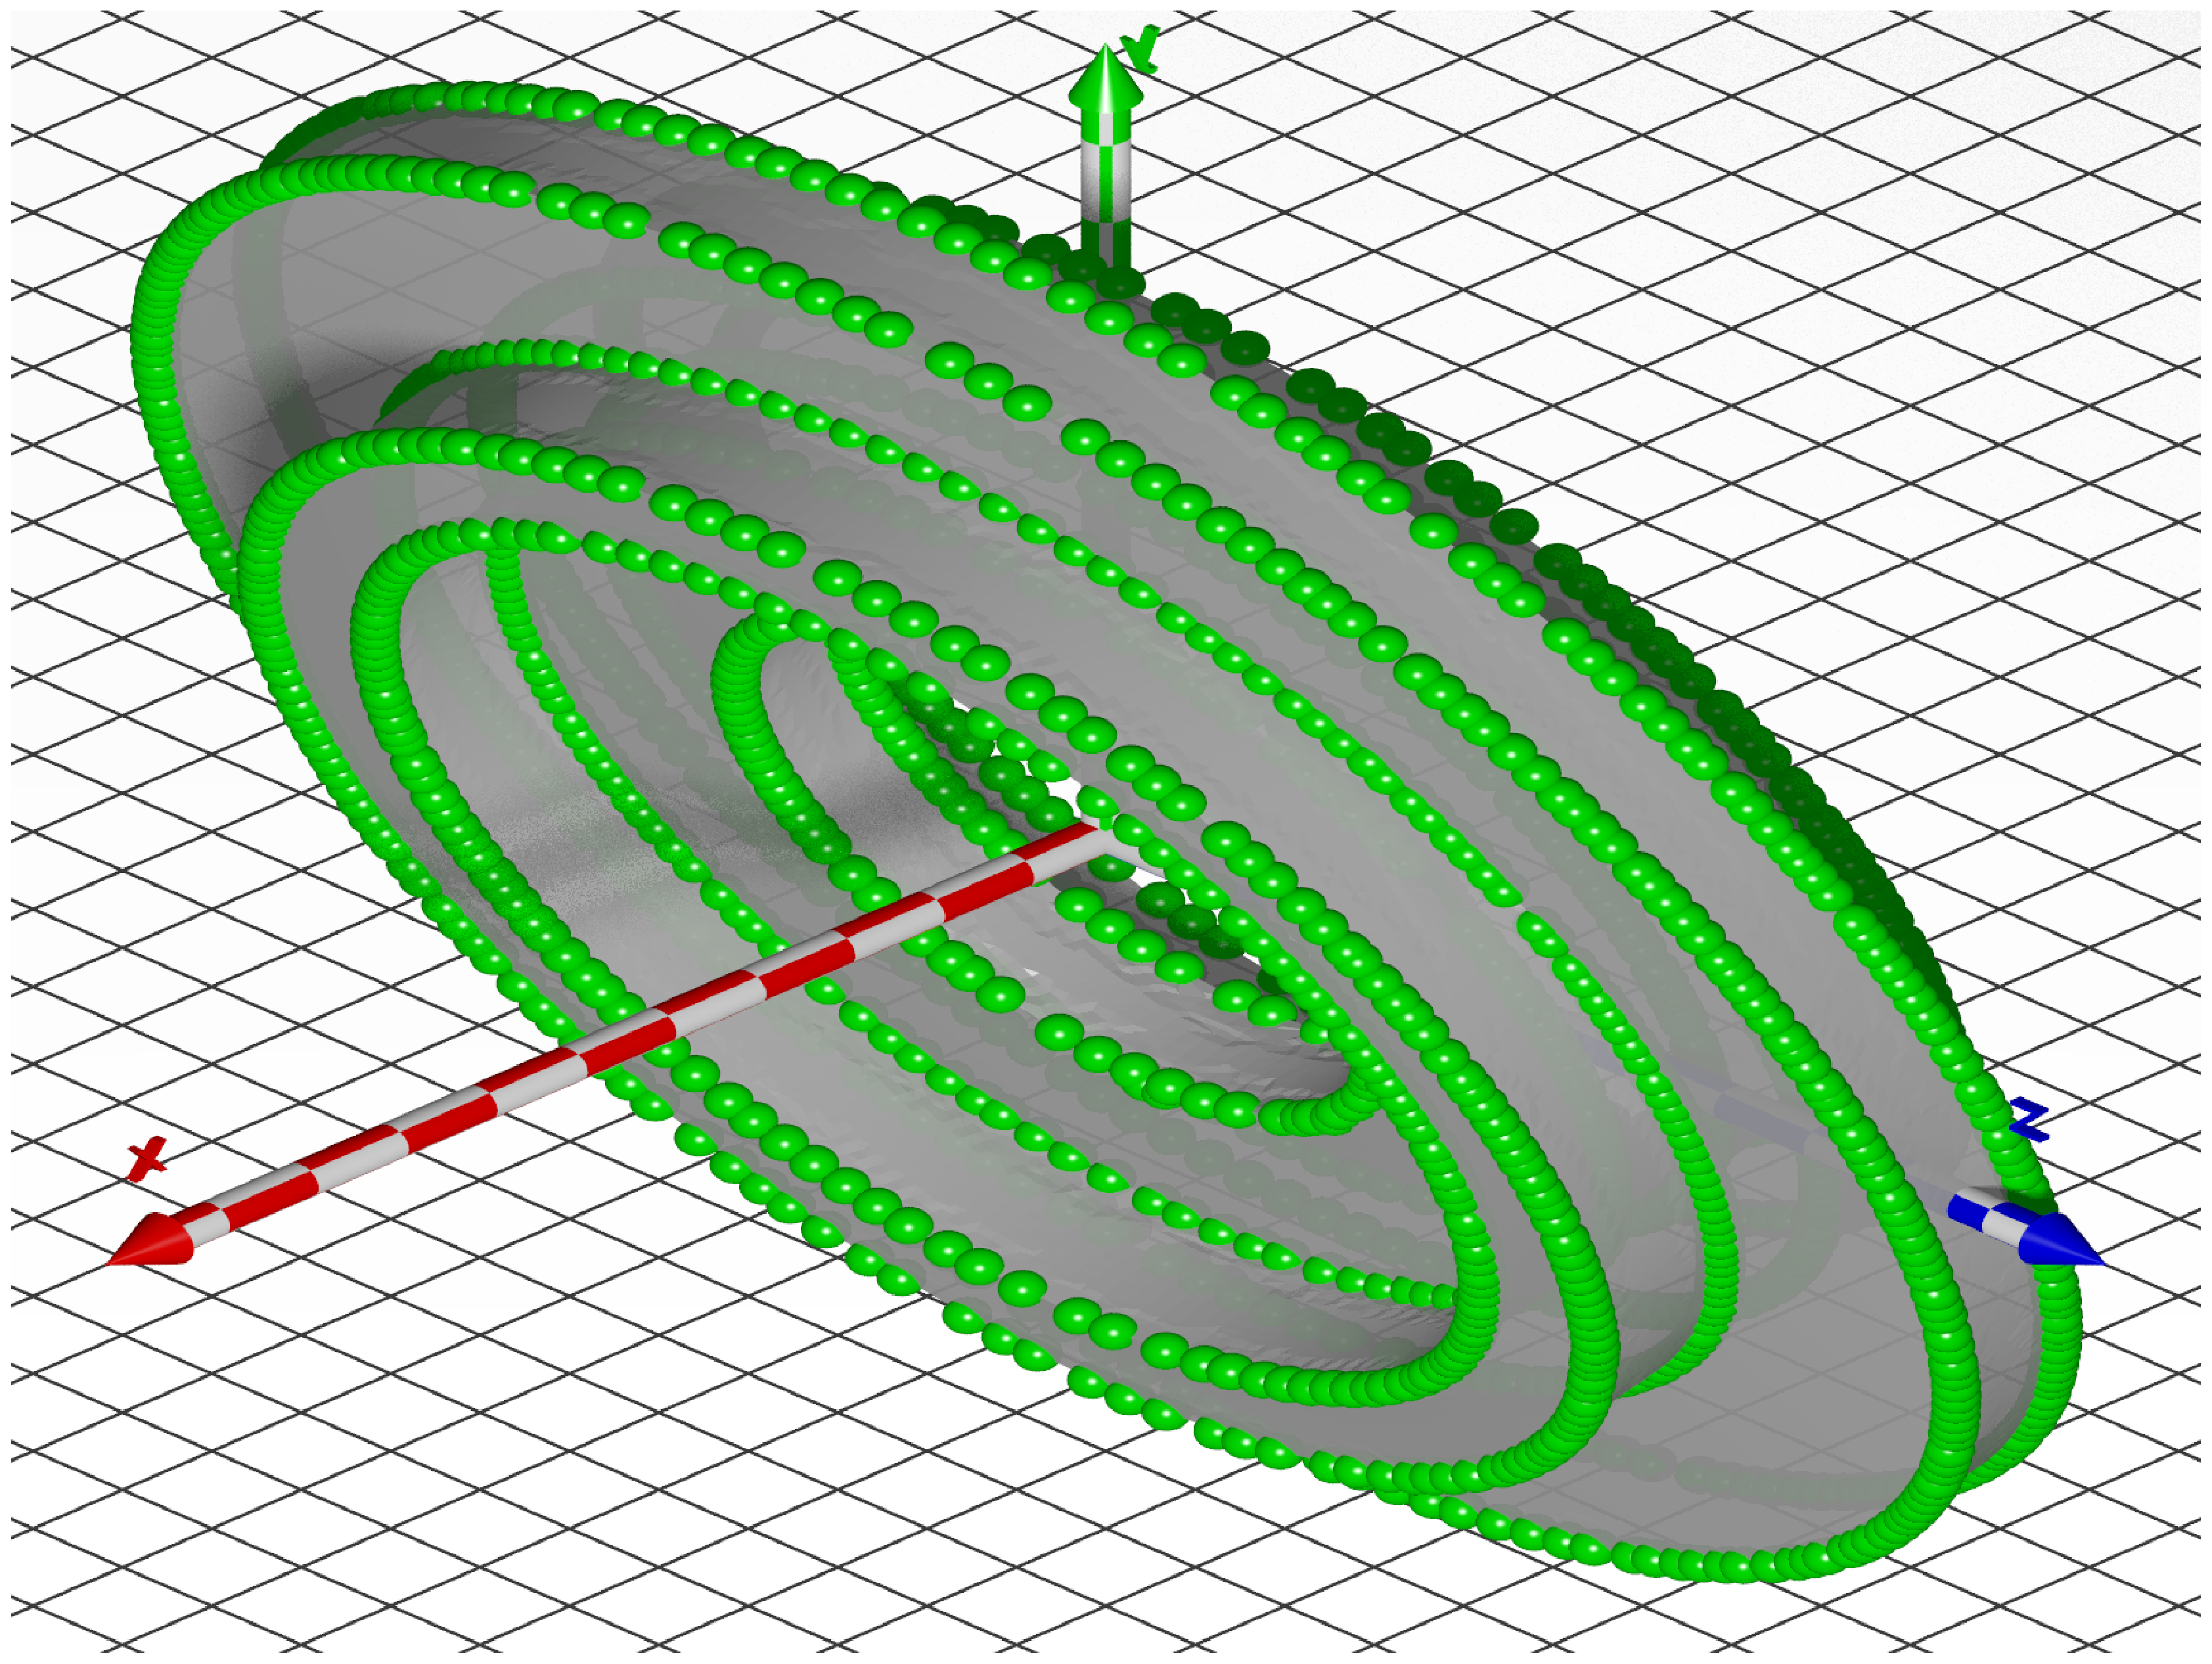
\includegraphics[width=0.2\linewidth]{images/flange.C2.new.eps}\label{fig:flange}}
%    \subfloat[Annulus]{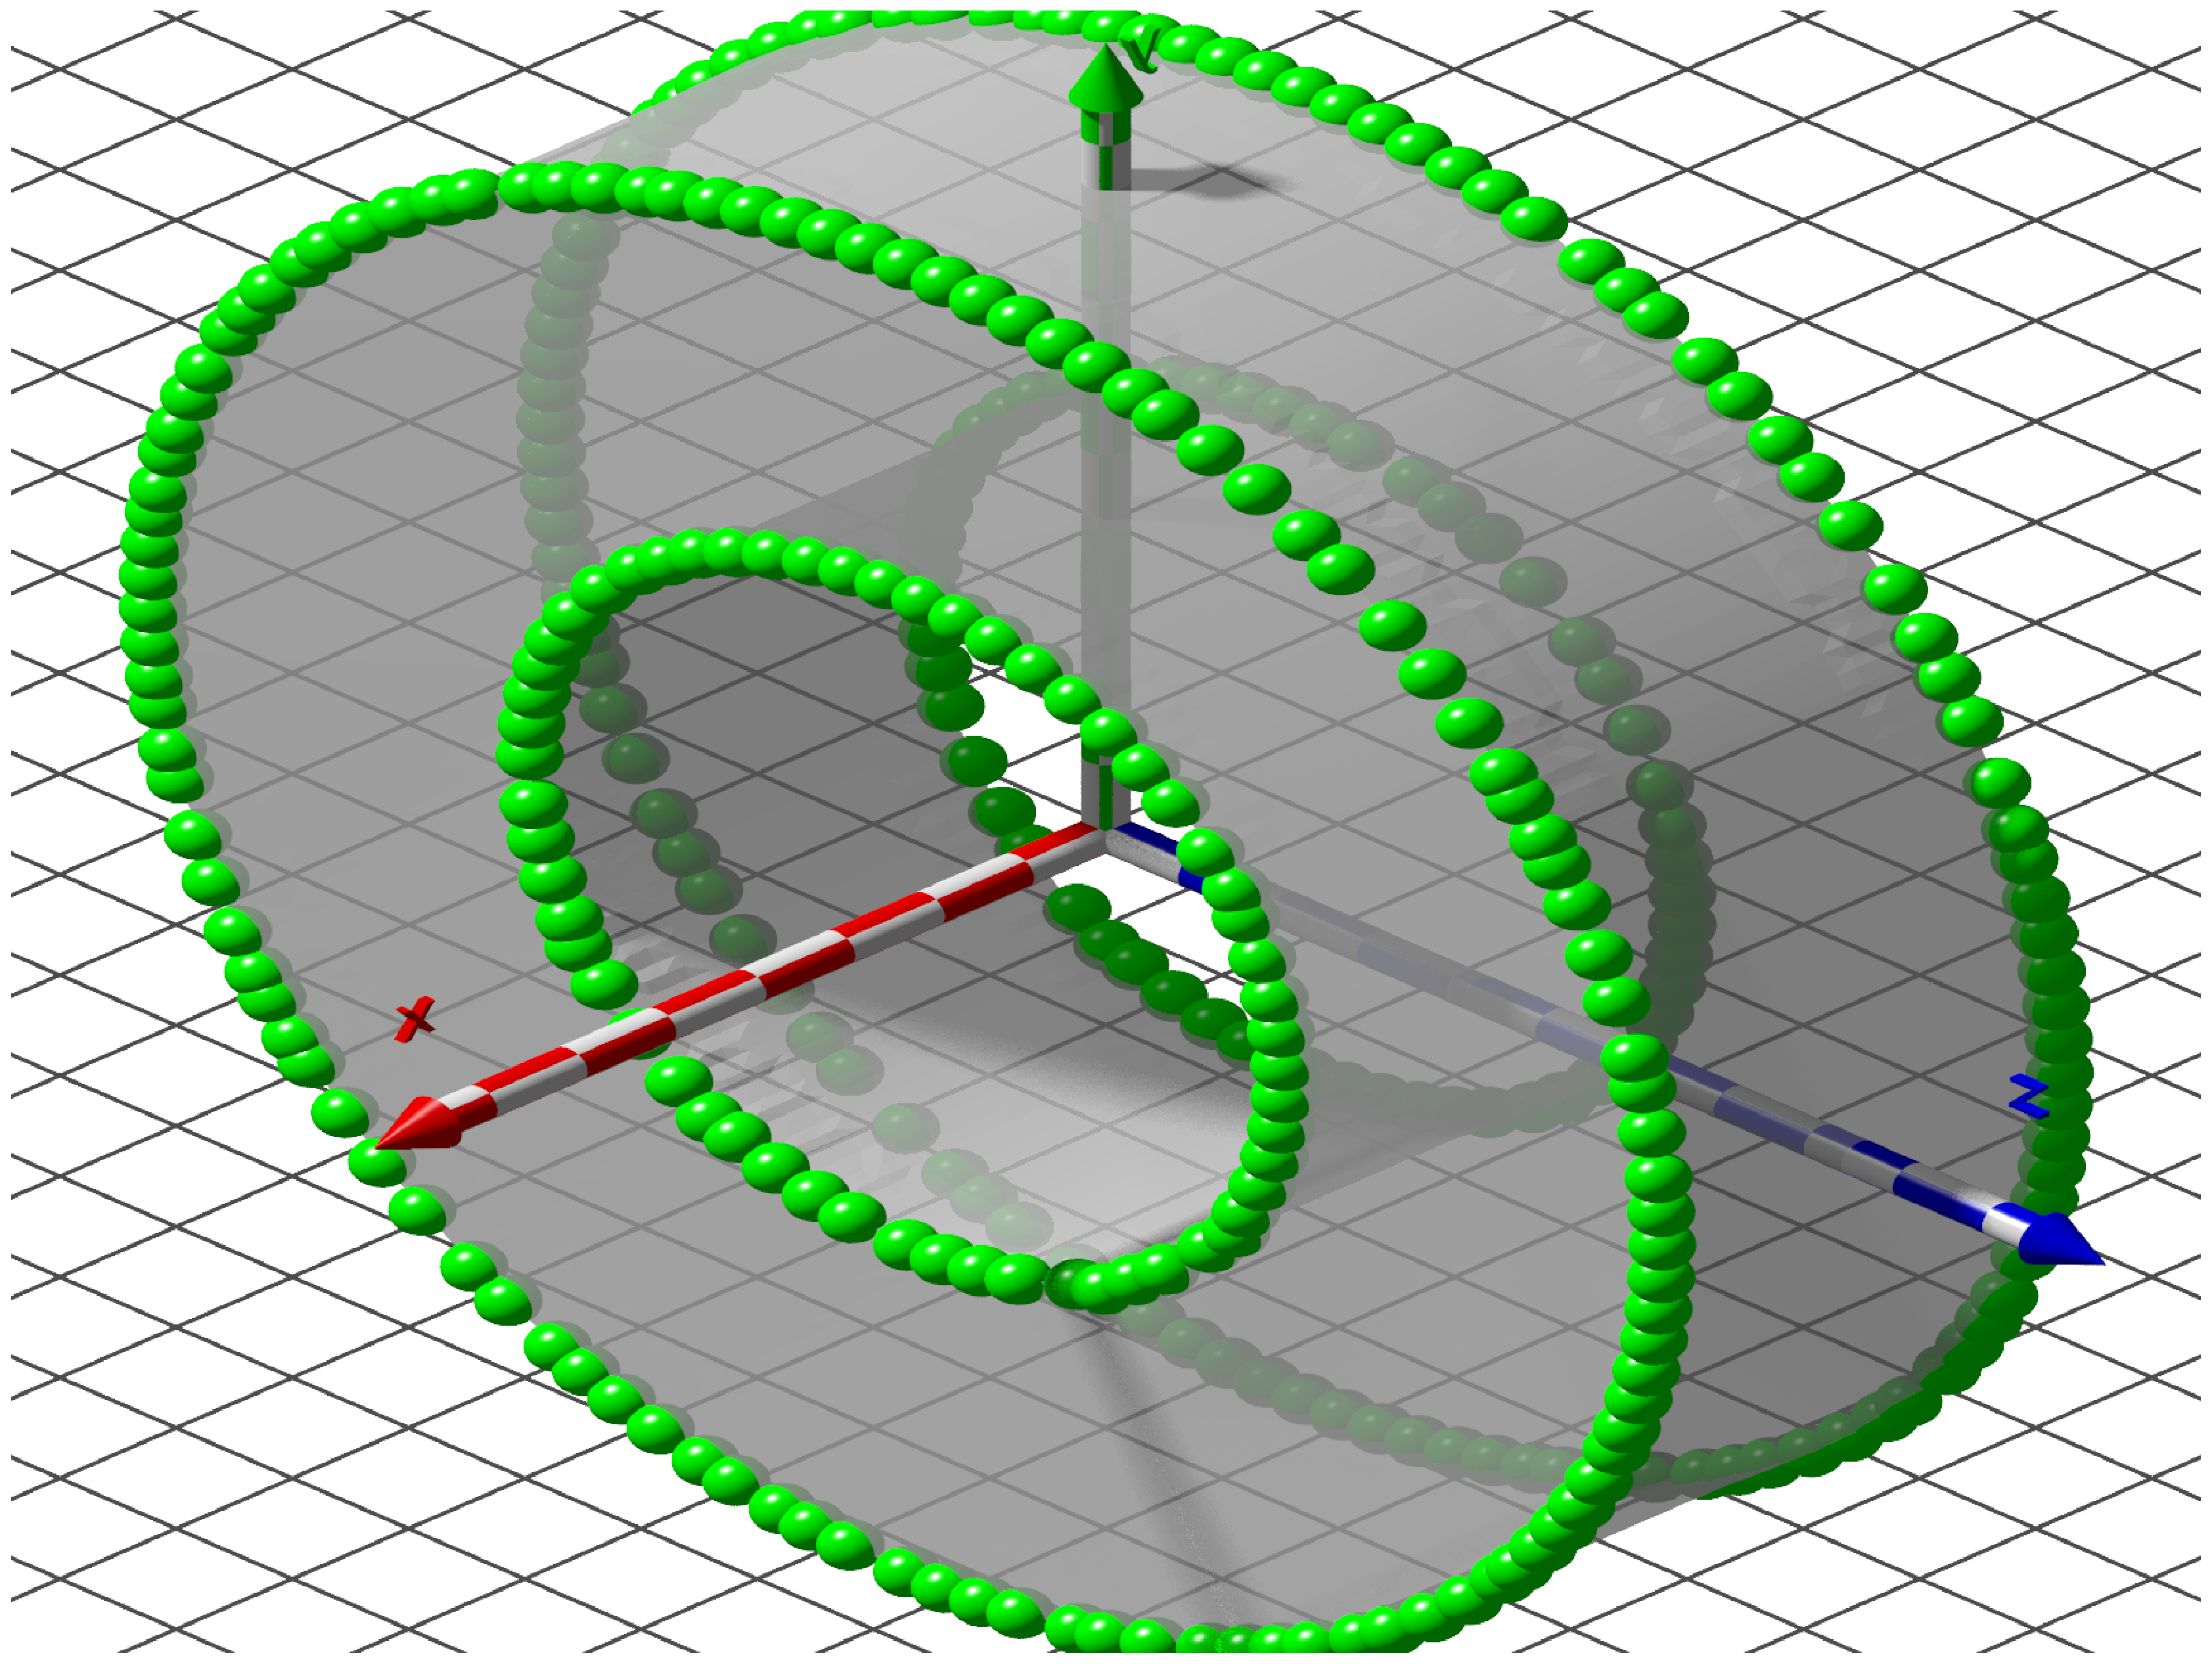
\includegraphics[width=0.2\linewidth]{images/annulus.eps}\label{fig:annulus}}
%    \subfloat[Cone]{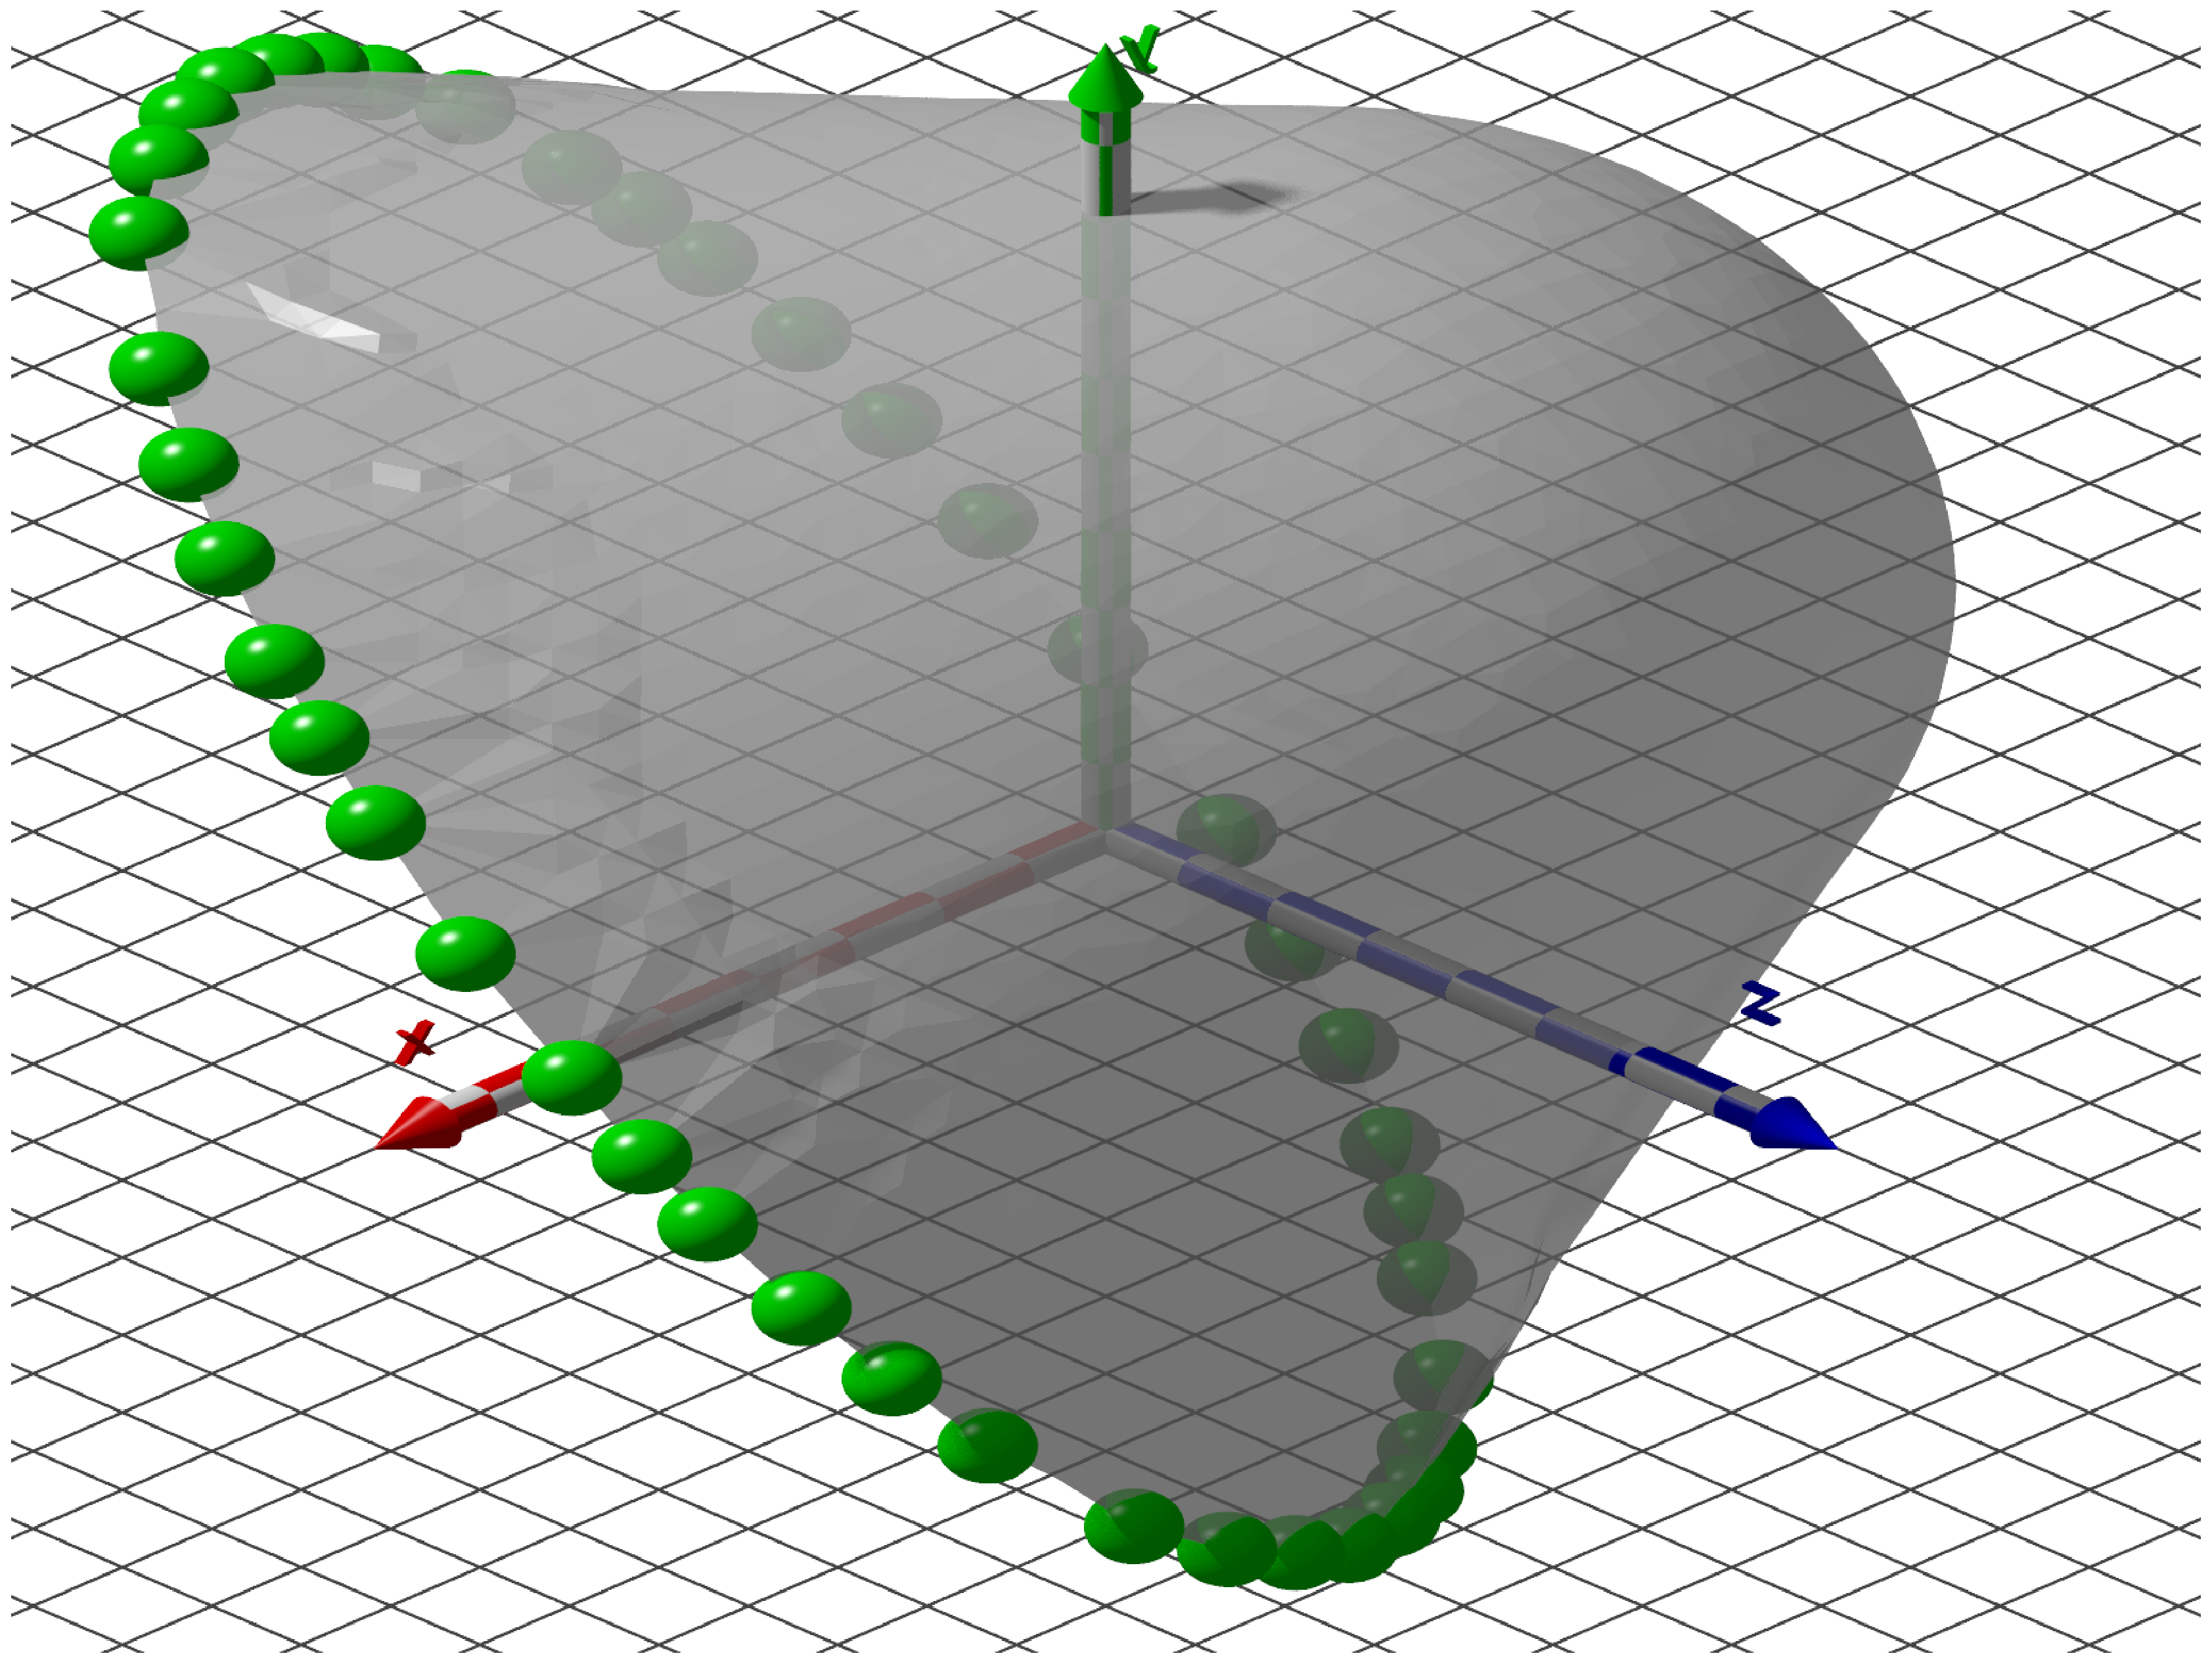
\includegraphics[width=0.2\linewidth]{images/cone.eps}\label{fig:cone}}
%    \subfloat[Cannon]{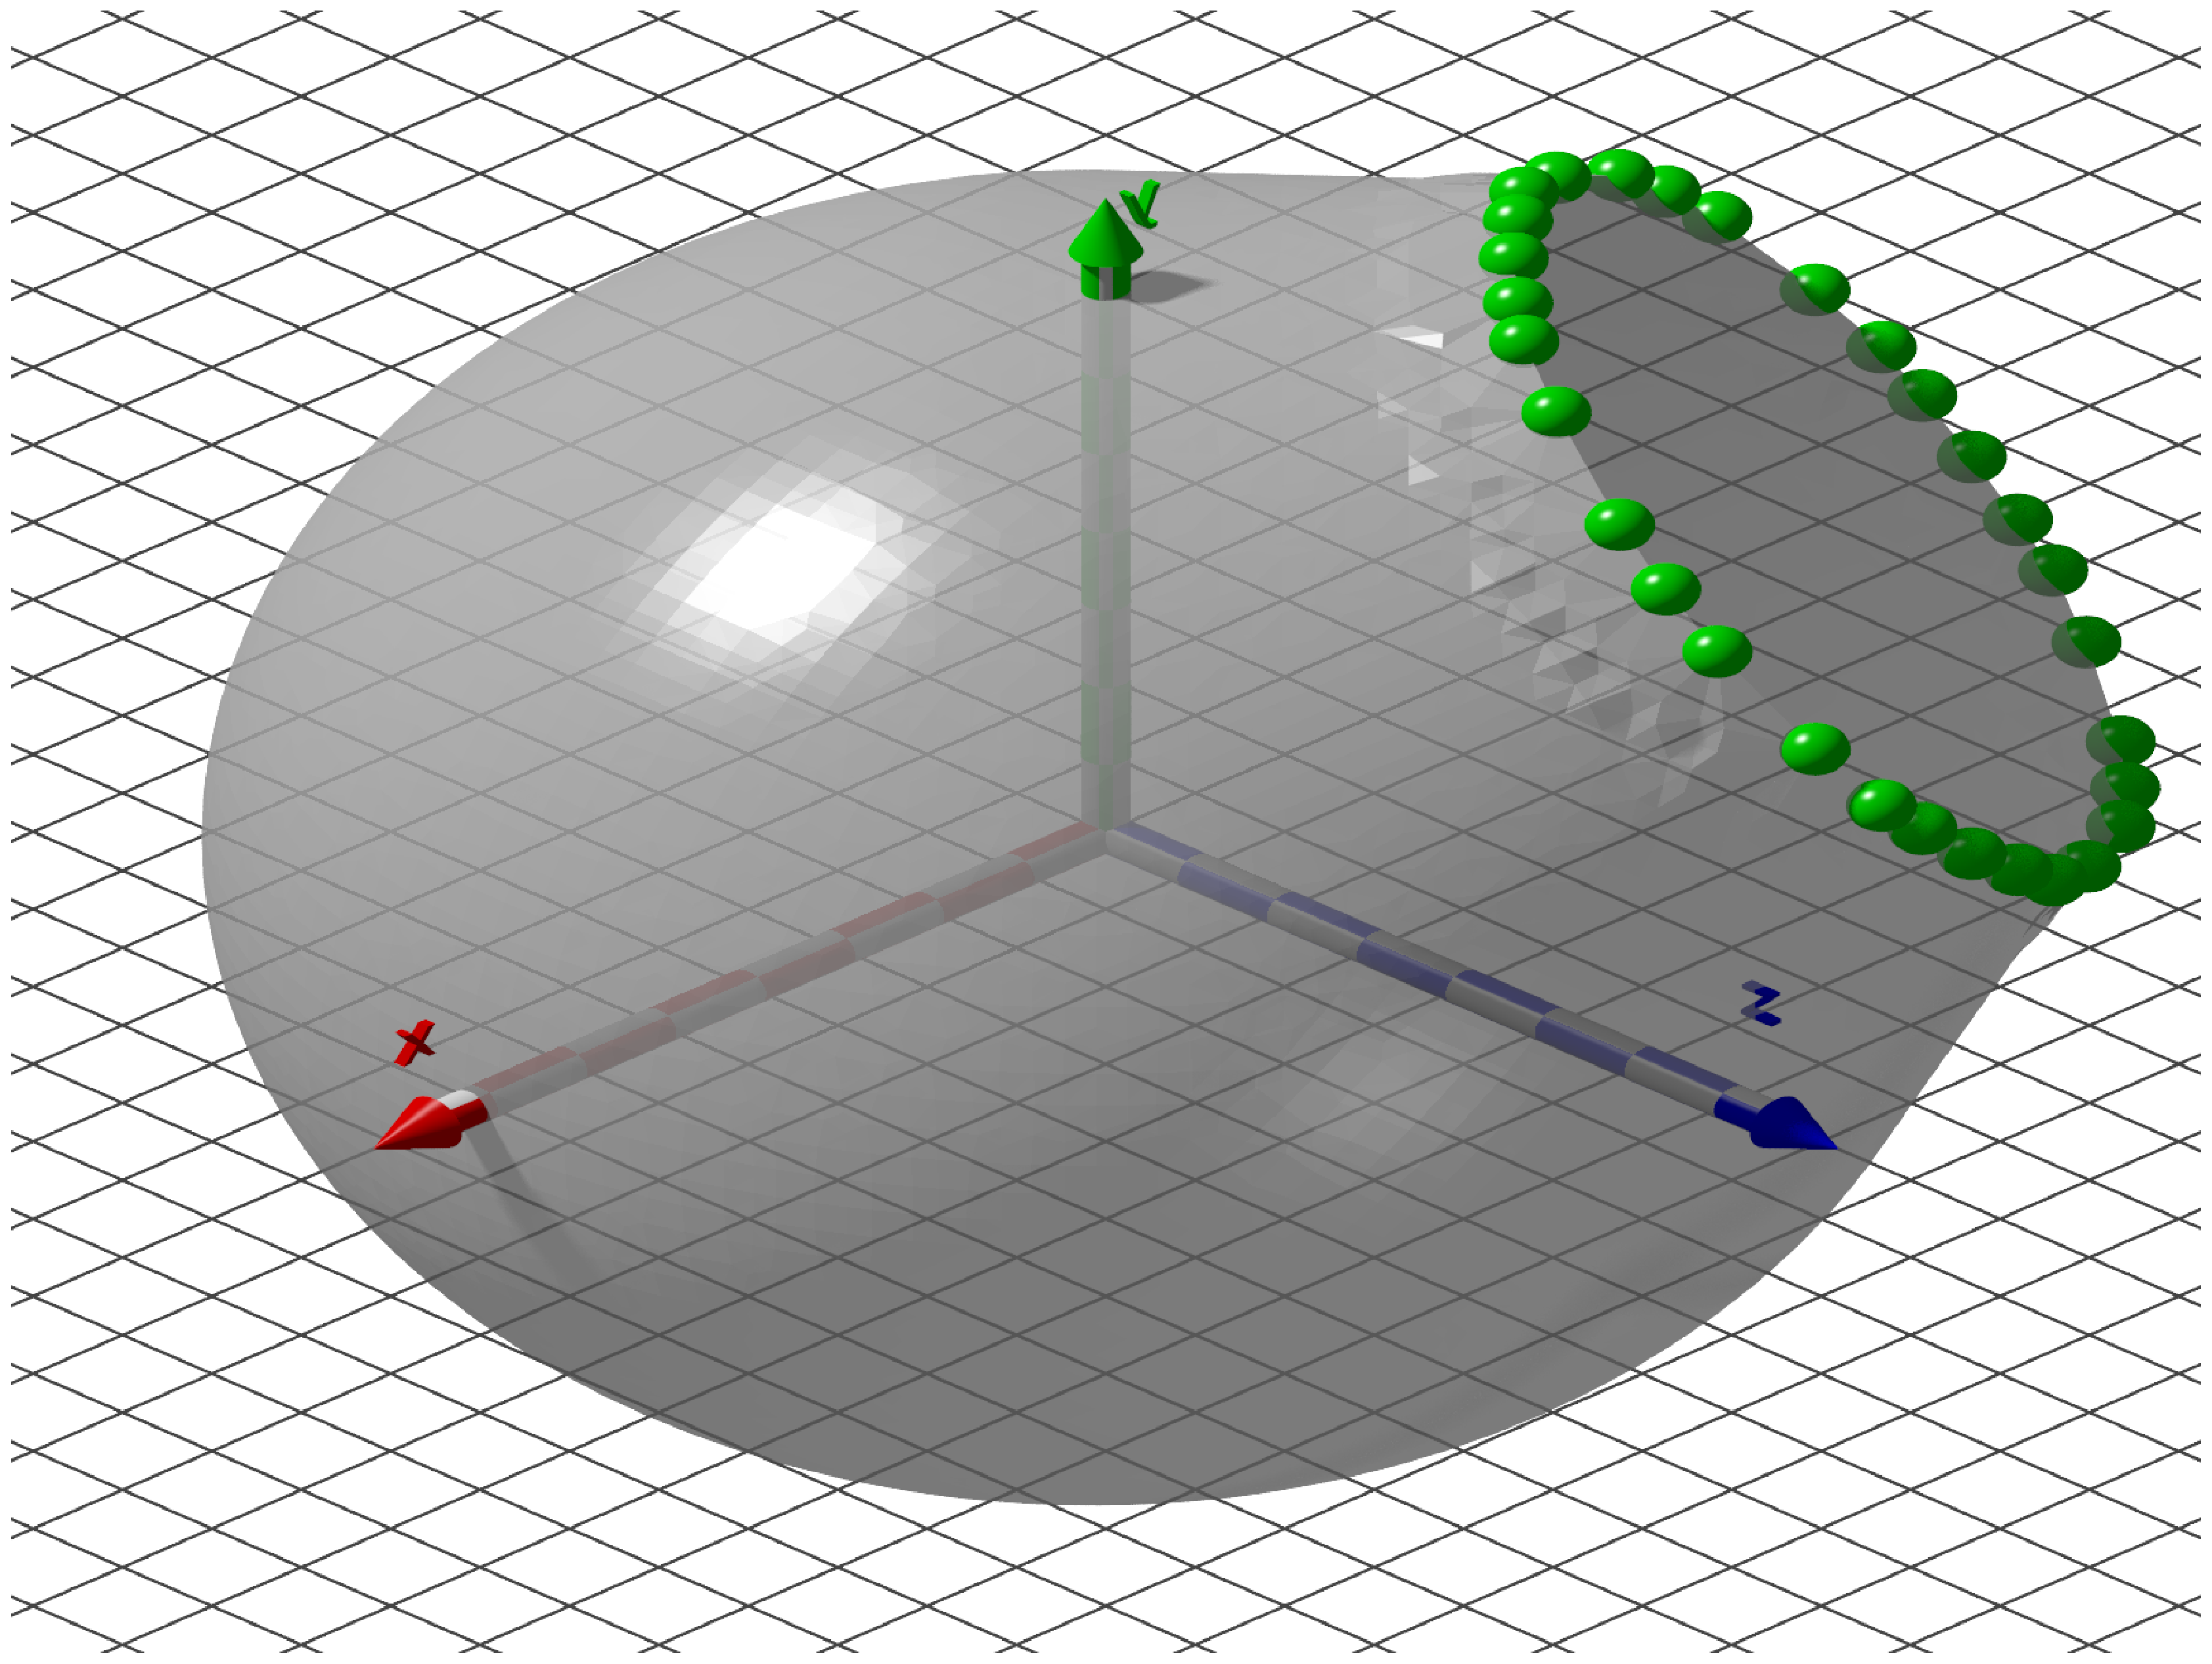
\includegraphics[width=0.2\linewidth]{images/cannon.eps}\label{fig:cannon}}
%    \caption{Synthetic datasets. Table~\ref{table:SynDataInfo} provides more information, Isosurface vertices associated with three large eigen values (Section~\ref{sec:computeSharpPoints}) are corners and marked in red. Selected edge isovertices are marked in green.}
%    \label{fig:SynData}
%\end{figure*}
\begin{table}[htb]
	\centering
	\begin{tabular}{|c c c c|} 
		\hline
		Name & ASize & Spacing & ARotation \\ [0.5ex] 
		\hline 
		\textit{Cube}  & 100 & 1 1 1 & 1 1 1\\
		\textit{Annulus} & 100 & 1 1 1 &  1 0 0\\ 
		\textit{TwoCube} & 150 & 0.2 0.2 0.4 &  1.732 0.577 0\\ 
		\textit{Flange} & 150 & 0.2 0.2 0.4 &  1.732 0.577 0\\ 
        \textit{Smooth-tip Cone} & 100 & 1 1 1 &  -1 1 1\\ 
        \textit{Cannon} & 100 & 1 1 1 &  -1 1 1\\ 
		\hline
	\end{tabular}

\caption{Synthetic dataset information, the size of the datasets is $ASize^3$. 
Each data set is centrally symmetric around the axis given by ARotation.
Faces of the \emph{Cube} and \emph{TwoCube} datasets are
orthogonal or parallel to the axis given by ARotation.}

	\label{table:SynDataInfo}
\end{table}
We tested our algorithm on a large number of synthetic datasets with varying spacings and axis rotations. 
Table \ref{table:SynDataInfo} and Figure~\ref{fig:SynData} show
six representative elements.

\textbf{Description}:
The \emph{Cube} dataset samples a scalar field $f:\colon\Rthree \to \R$, where $f(p)$ is the minimum of the $L_{\infty}$ distance to a single point. Tilted cubes are made from orthogonal frames other than the standard \emph{x,y} and \emph{z} axis. 
The isosurfaces in the \emph{TwoCube} dataset contain sharp corners
and sharp saddle points.
The \emph{Annulus} dataset is minimum of the distance to a cylinder and the distance to a plane orthogonal to the cylinder.
By adding constants to these distances, we can create annulli with arbitrary heights and radii.
The \emph{Flange} datasets is the minimum of two \emph{Annulus} data sets,
one with flat, wide annulii and one with tall thin annulii.
Isosurfaces in these datasets are flanges with sharp concave and convex edges.
The \emph{Cone} data set is the minimum of the distance to a cone and to an orthogonal plane.
The distance to the cone near the tip is the distance to the point at the tip of the cone.
The isosurface around the tip is part of a sphere.
The \emph{Cone} dataset has acute dihedral angles of $60^\circ$.
The \emph{Cannon} dataset is the combination of the distance to a cone, the distance to an orthogonal plane
and the distance to a point.
The \emph{Cannon} dataset has obtuse dihedral angles of $120^\circ$.
\emph{Flange} and \emph{TwoCube} are challenging datasets, the spacings on these are not uniform and they are not axis aligned.
\emph{Cone} and \emph{Cannon} are also not axis aligned (Table\ref{table:SynDataInfo}).

%\begin{figure*}[tb]
%    \centering
%    \subfloat[Correct Gradients]{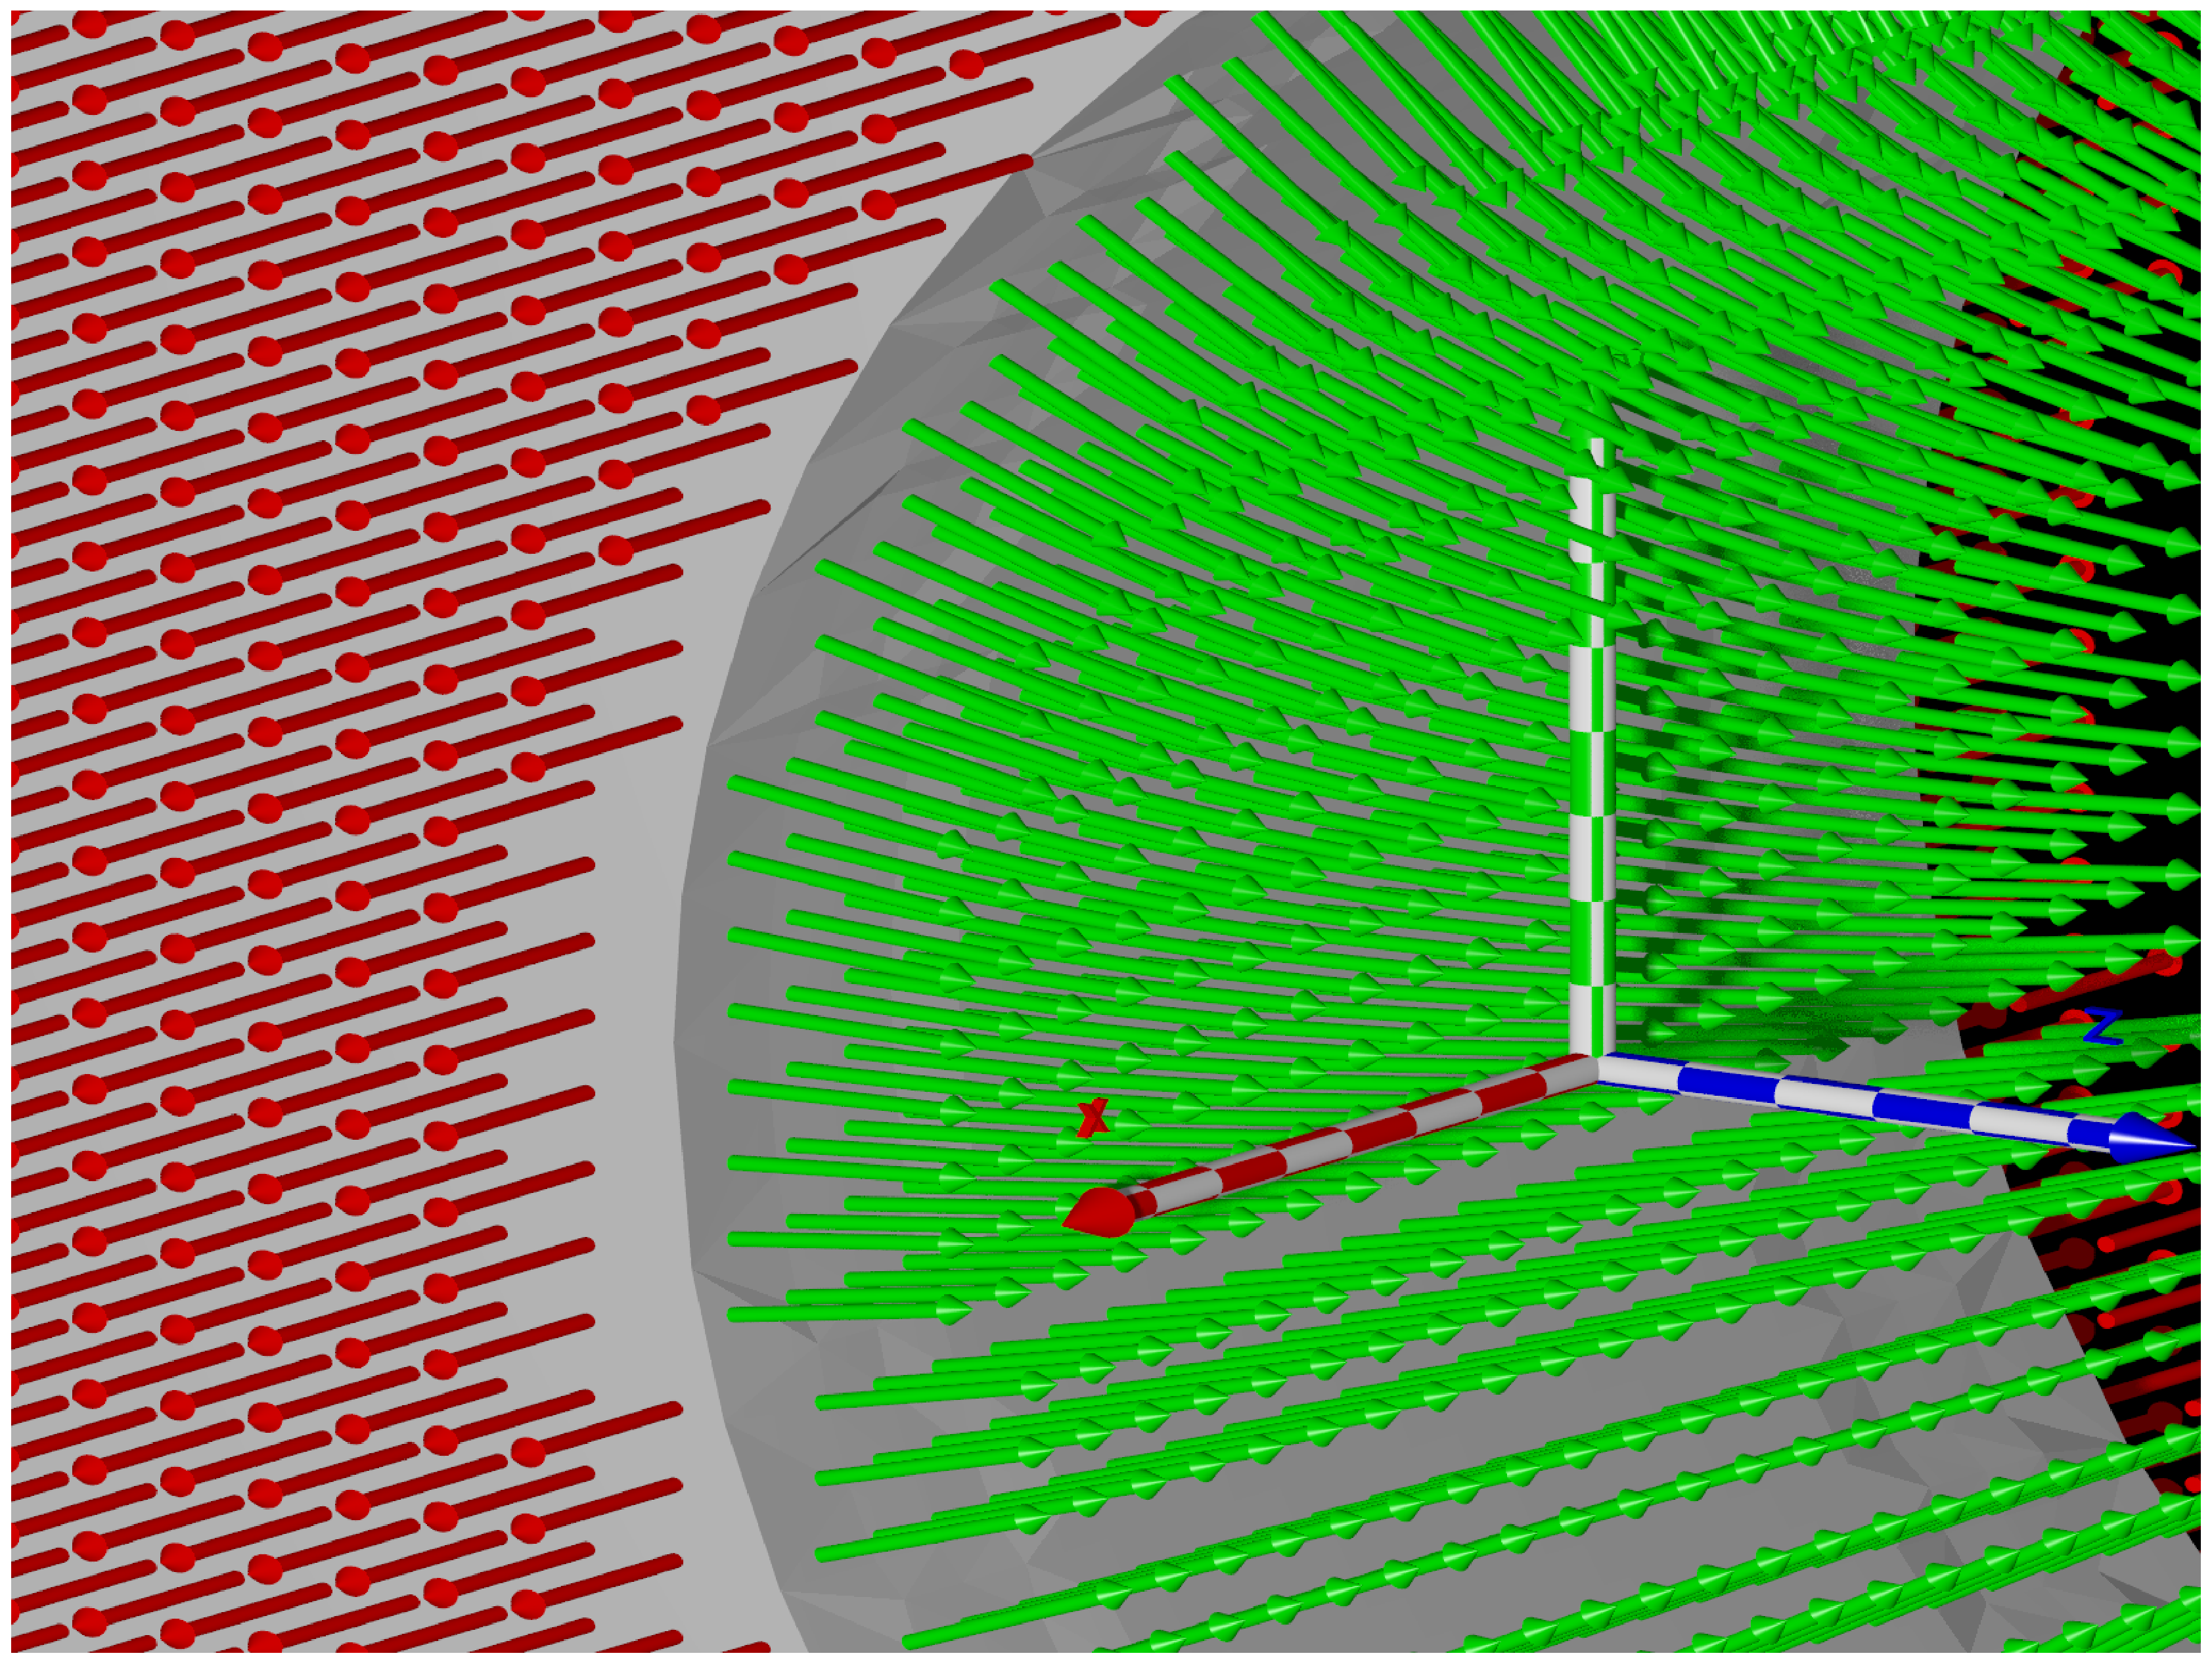
\includegraphics[height=0.2\linewidth]{images/annulus.gradcompare.correct.eps}\label{fig:annulus:correct}}\quad
%    \subfloat[Edge dist. 1 predictions]{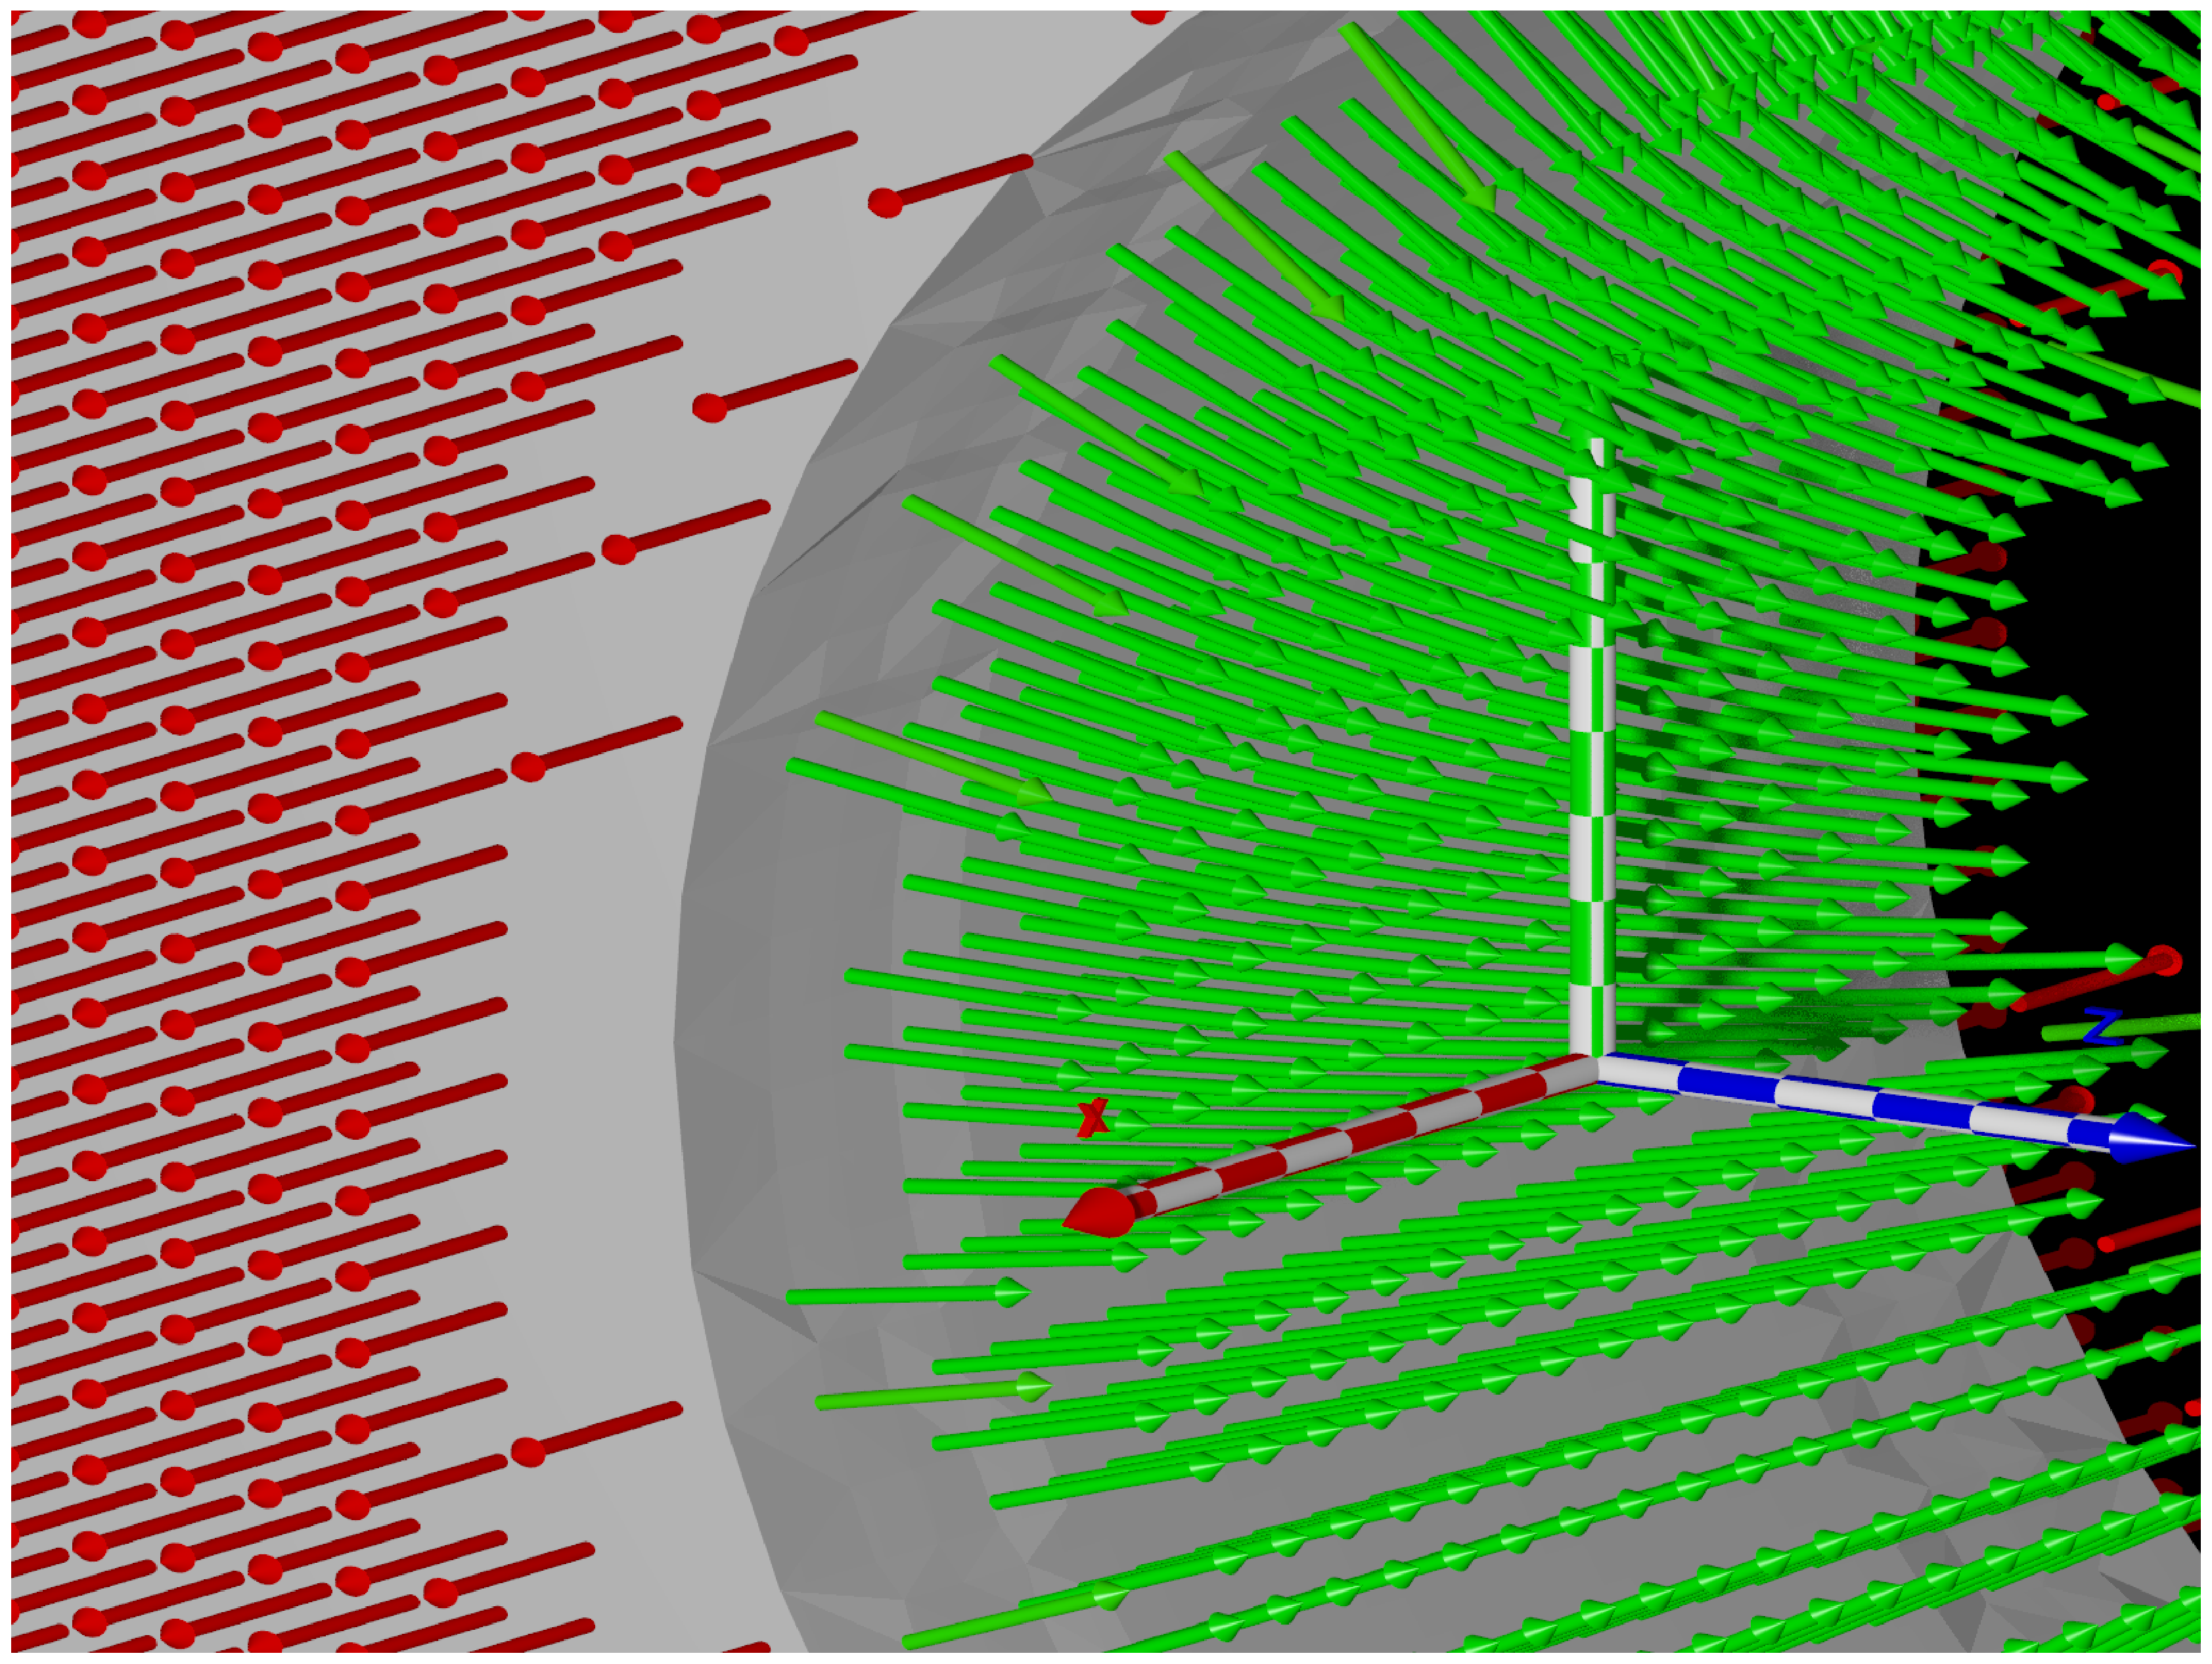
\includegraphics[height=0.2\linewidth]{images/annulus.gradcompare.algo1.eps}\label{fig:annulus:algo1} }\quad
%    \subfloat[Edge dist. 2 predictions]{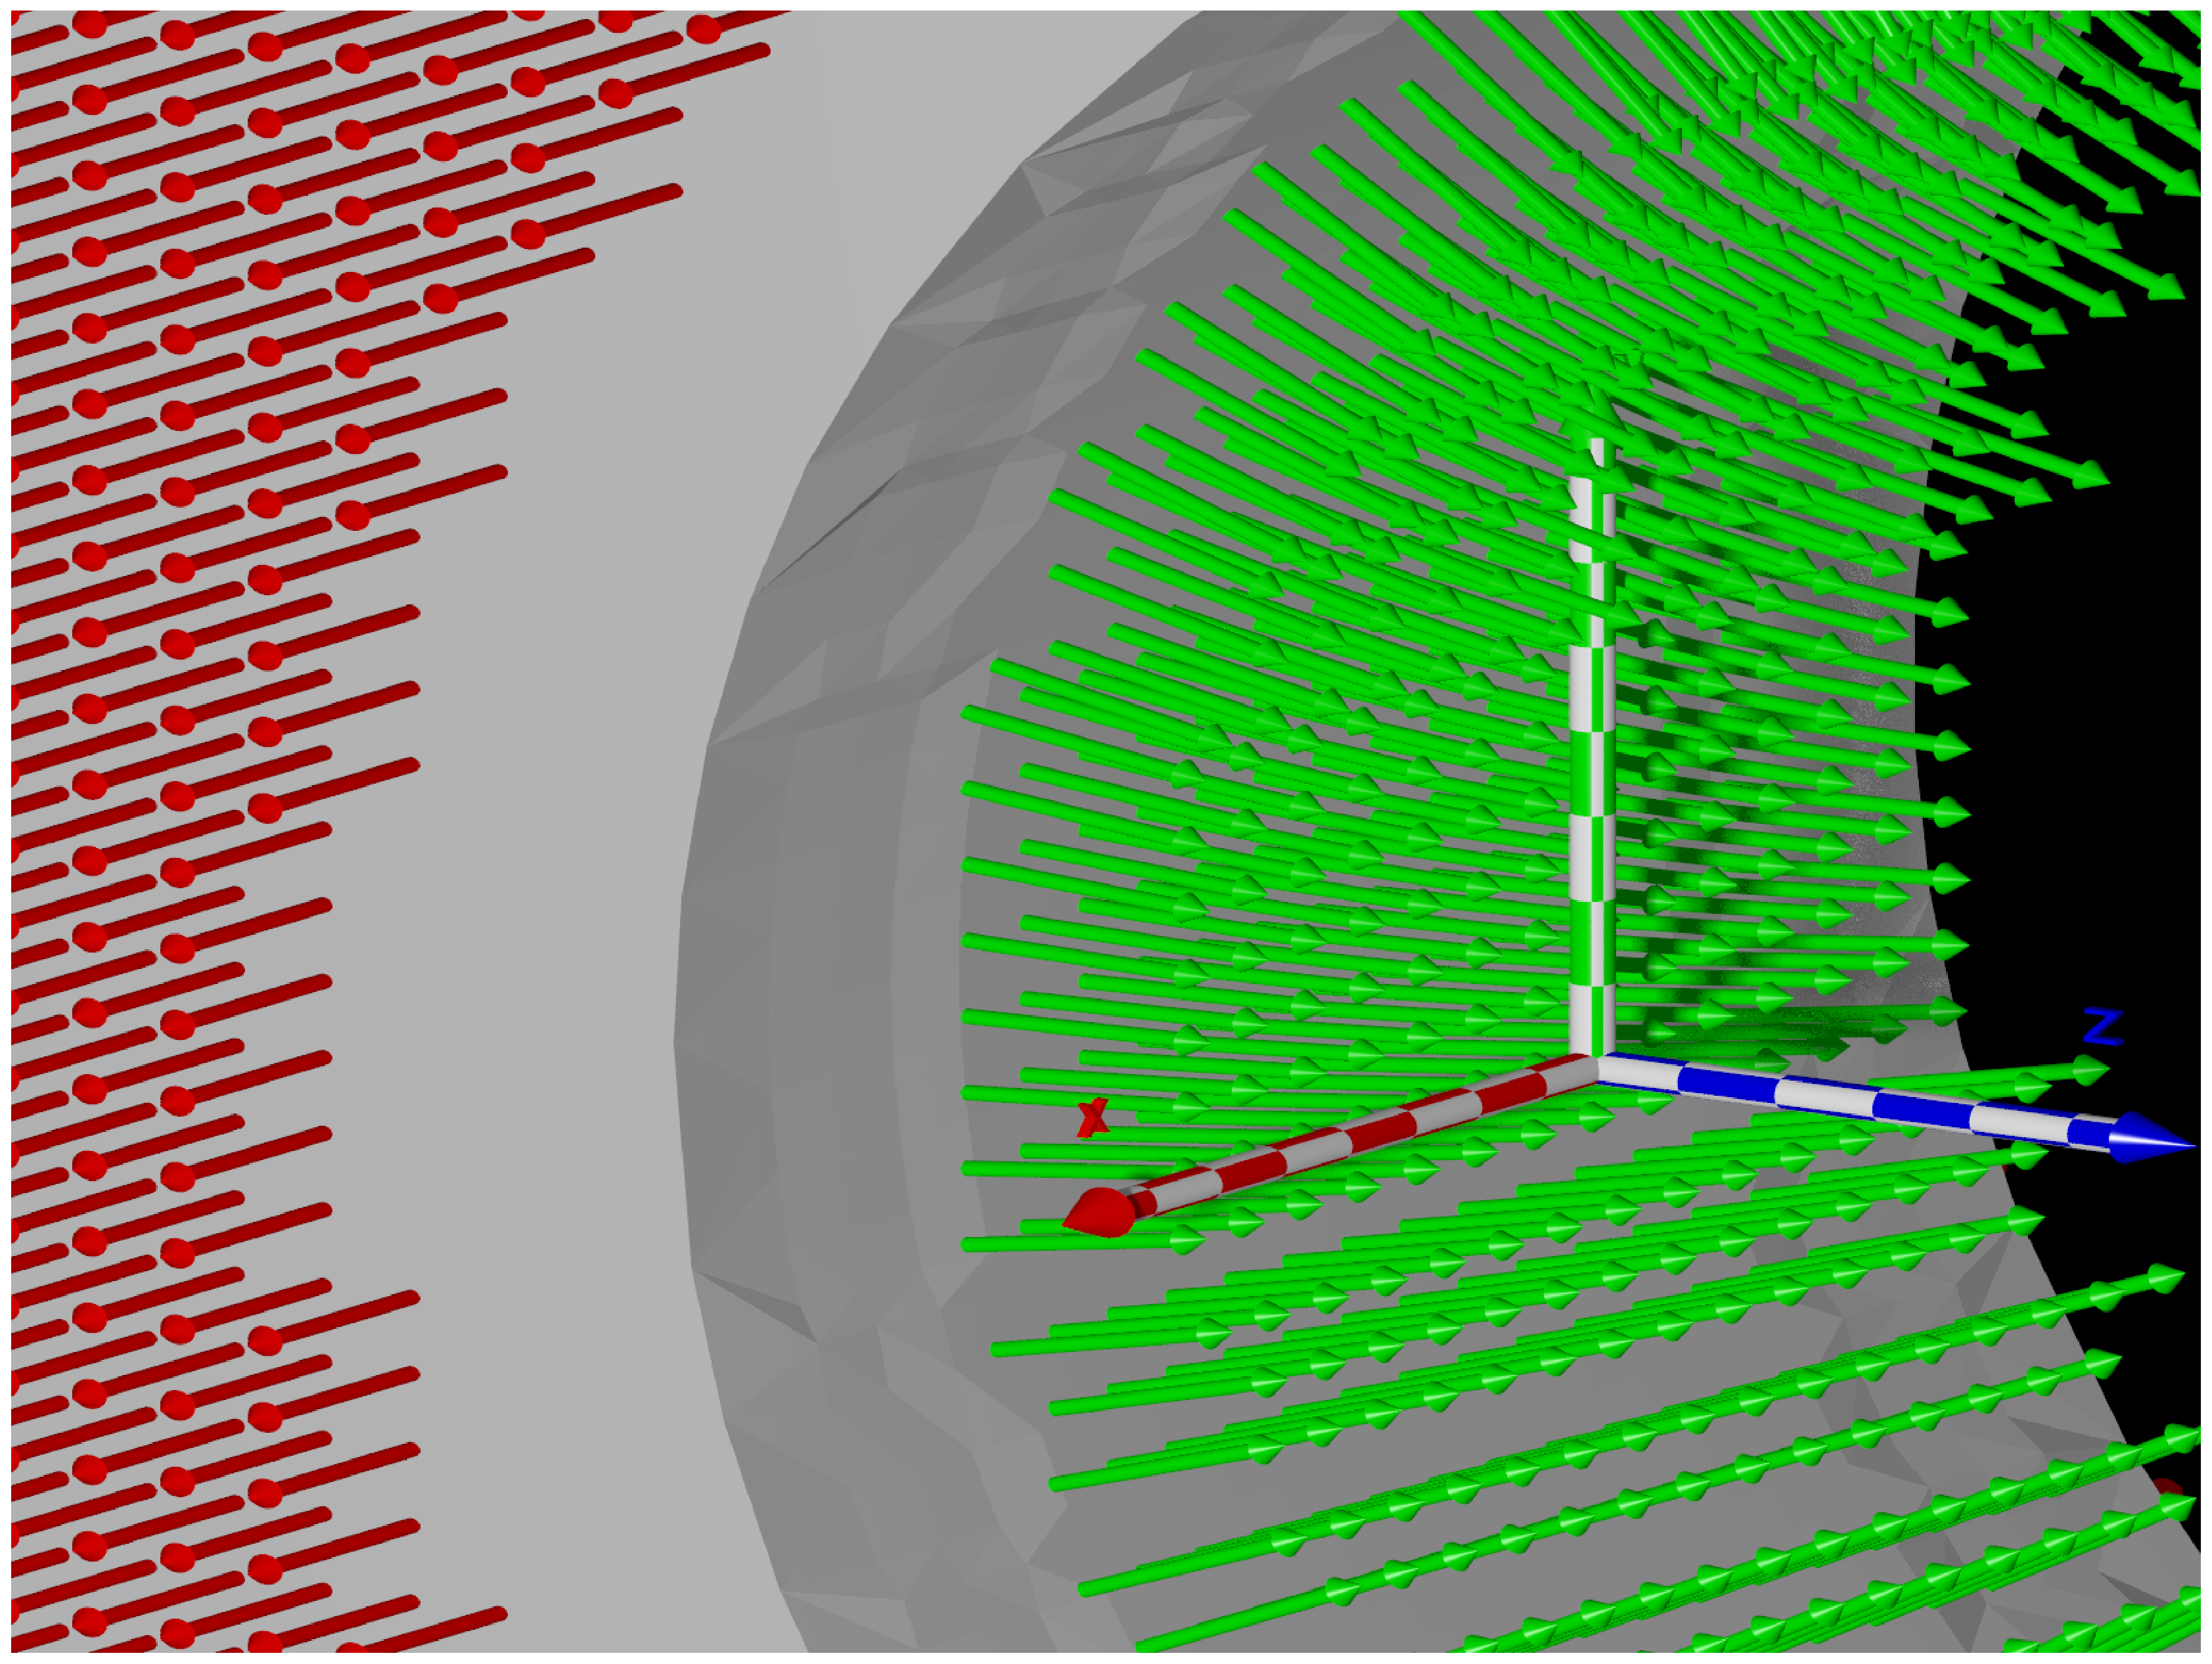
\includegraphics[height=0.2\linewidth]{images/annulus.gradcompare.algo2.eps}\label{fig:annulus:algo2}}
%    \subfloat[Central Difference]{\includegraphics[height=0.2\linewidth]{images/gradCompare.full.A.eps}\label{fig:annulus:cdiff} }
%    \subfloat[ReliGrad]
%    {\includegraphics[height=0.2\linewidth]{images/gradCompare.full.B.eps}\label{fig:annulus:religrad} }\vspace{-3mm}
%    \caption{Gradient results on a part of the \emph{Annulus} dataset (Figure~\protect\subref*{fig:annulus}).
%     \protect\subref{fig:annulus:correct} Correct gradients.
%     \protect\subref{fig:annulus:algo1}  Gradients marked correct by Algorithm 1 which uses $n_{v''}$ and $n_{v'}$ to predict $n_v$.
%     \protect\subref{fig:annulus:algo2} Gradients marked correct by Algorithm 2 which uses $n_{v'''}$, $n_{v''}$, and $n_{v'}$ to predict $n_v$.
%     \protect\subref{fig:annulus:cdiff} Central difference gradients. The blue inset on the right contains a magnified view. 
%     \protect\subref{fig:annulus:religrad} Gradients marked correct by \protect\ReliGrad. The cyan inset shows a magnified view.
%     }    
%\label{fig:annulus:gradResults}
%\end{figure*}

\begin{figure}[tb]
    \centering
    \subfloat[Correct Gradients]{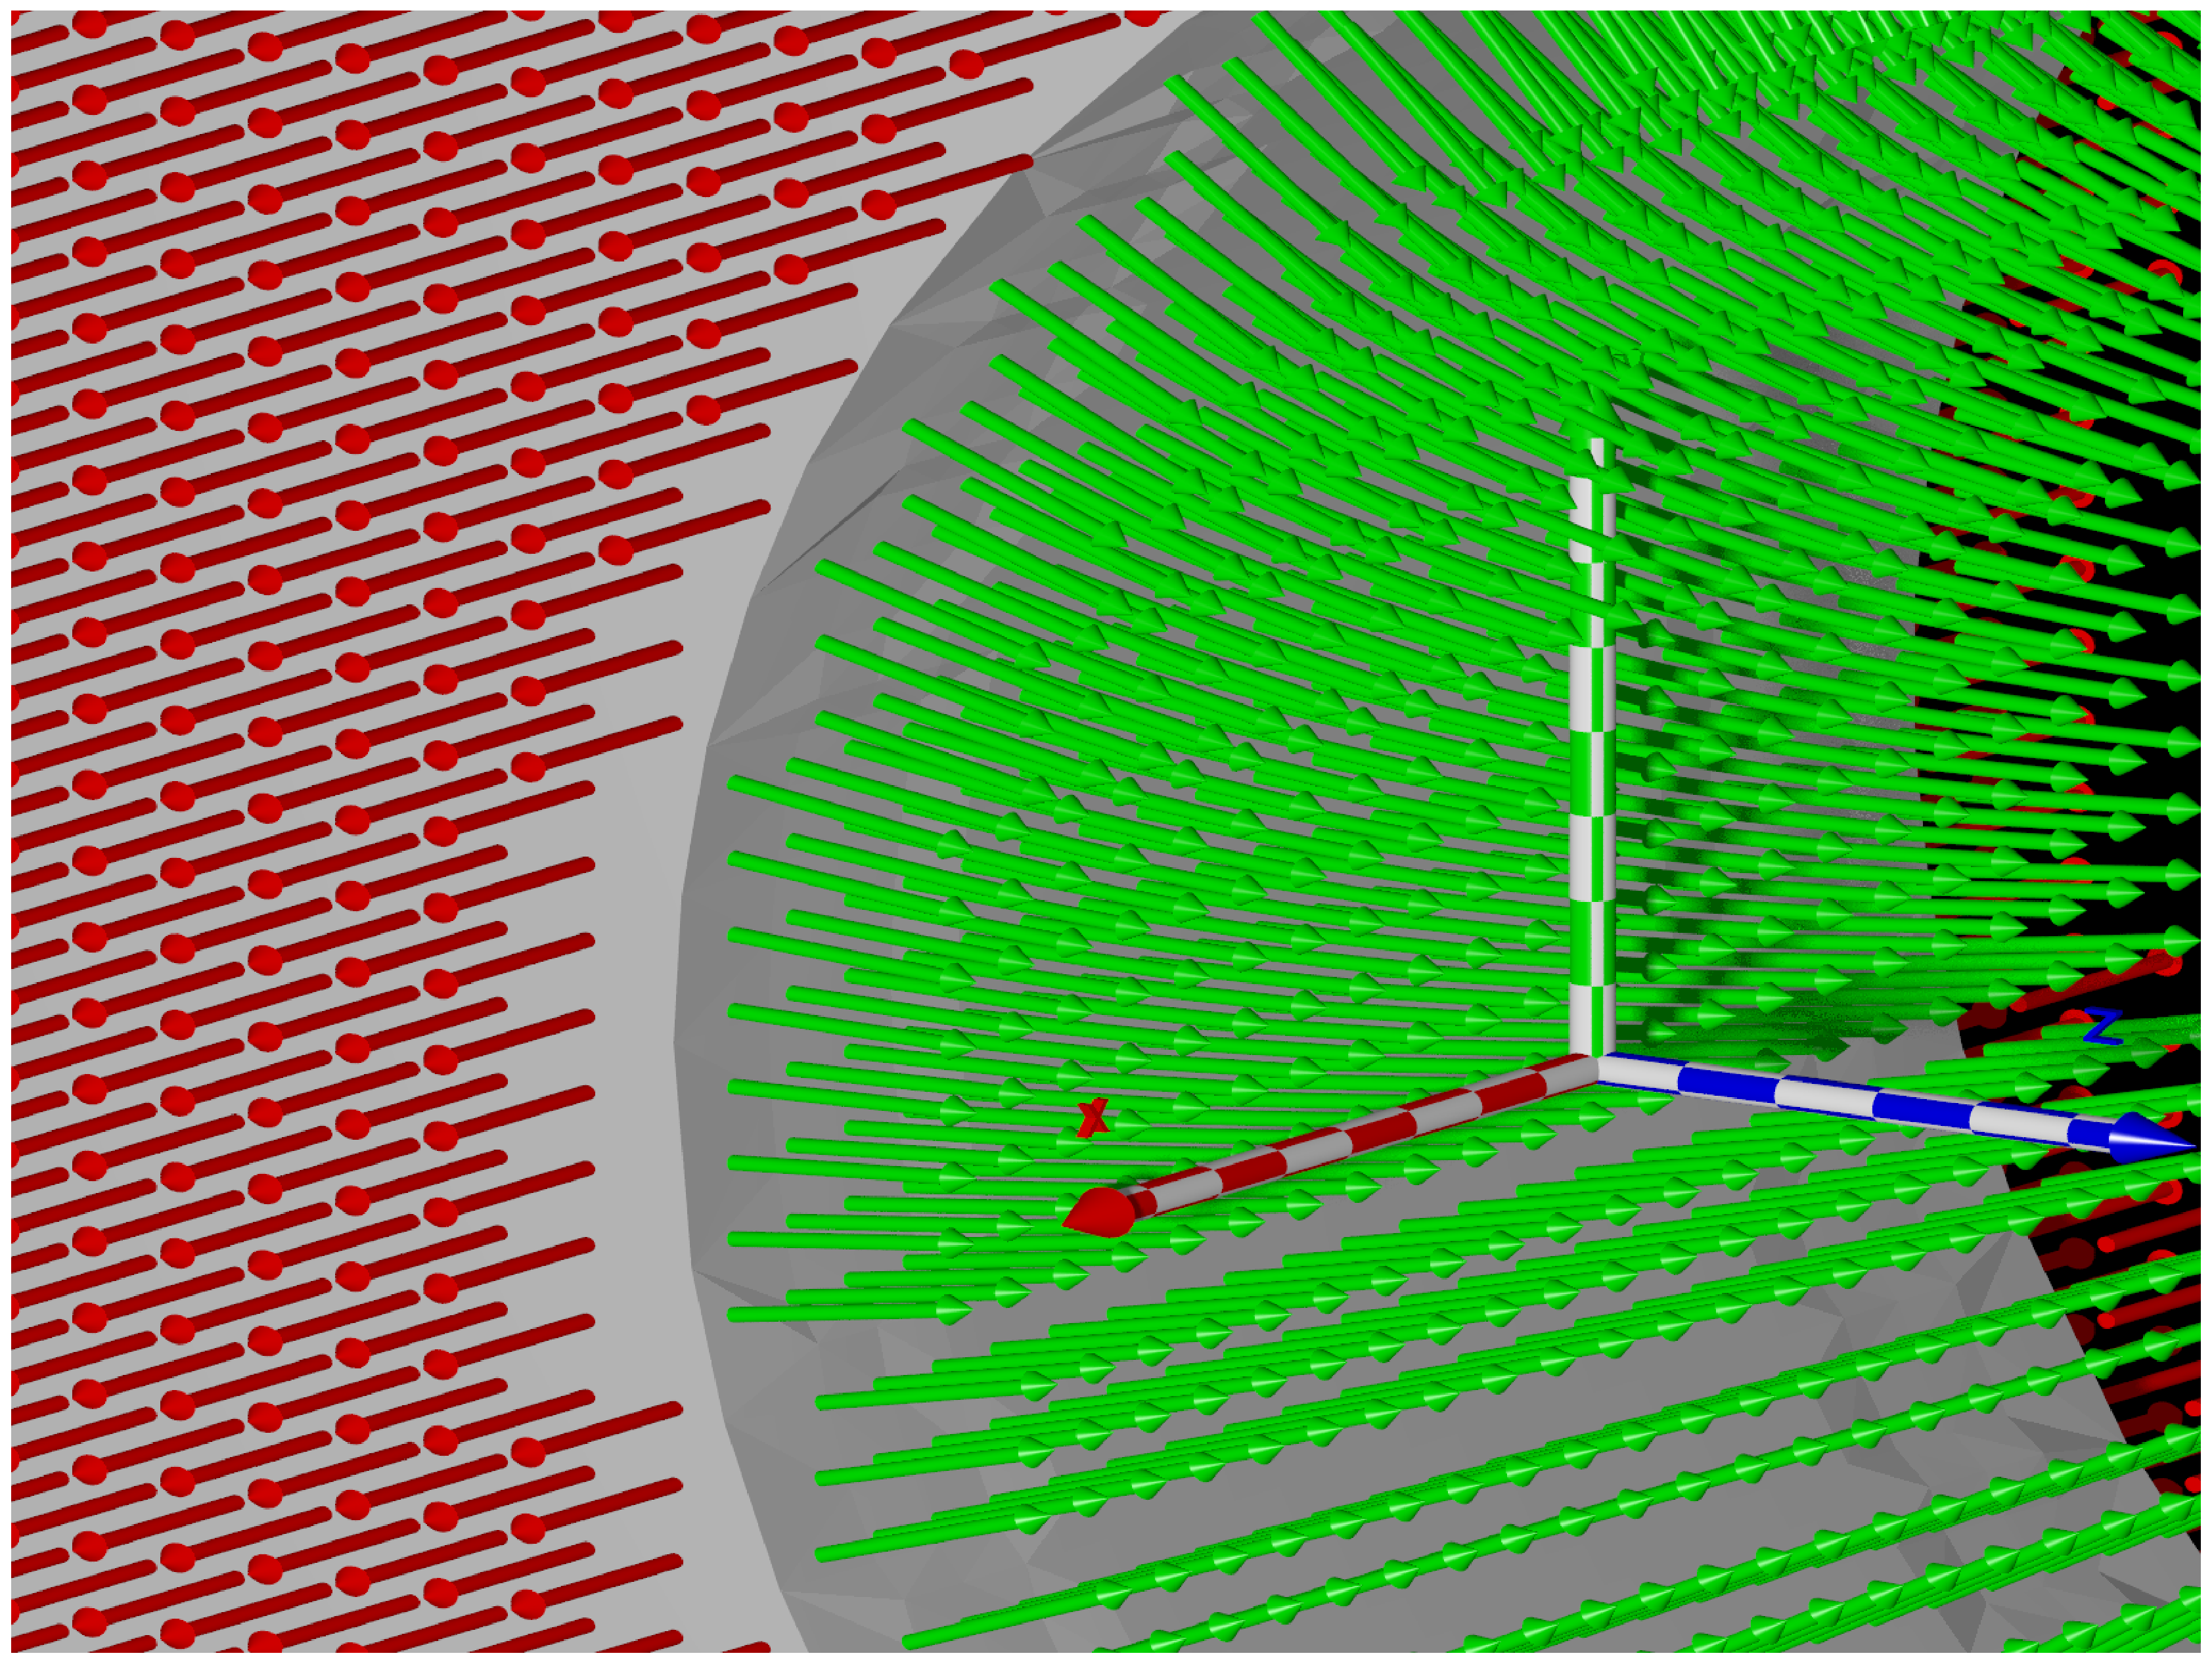
\includegraphics[width=0.33\linewidth]{images/annulus.gradcompare.correct.eps}\label{fig:annulus:correct}}
    \subfloat[Edge dist. 1 predictions]{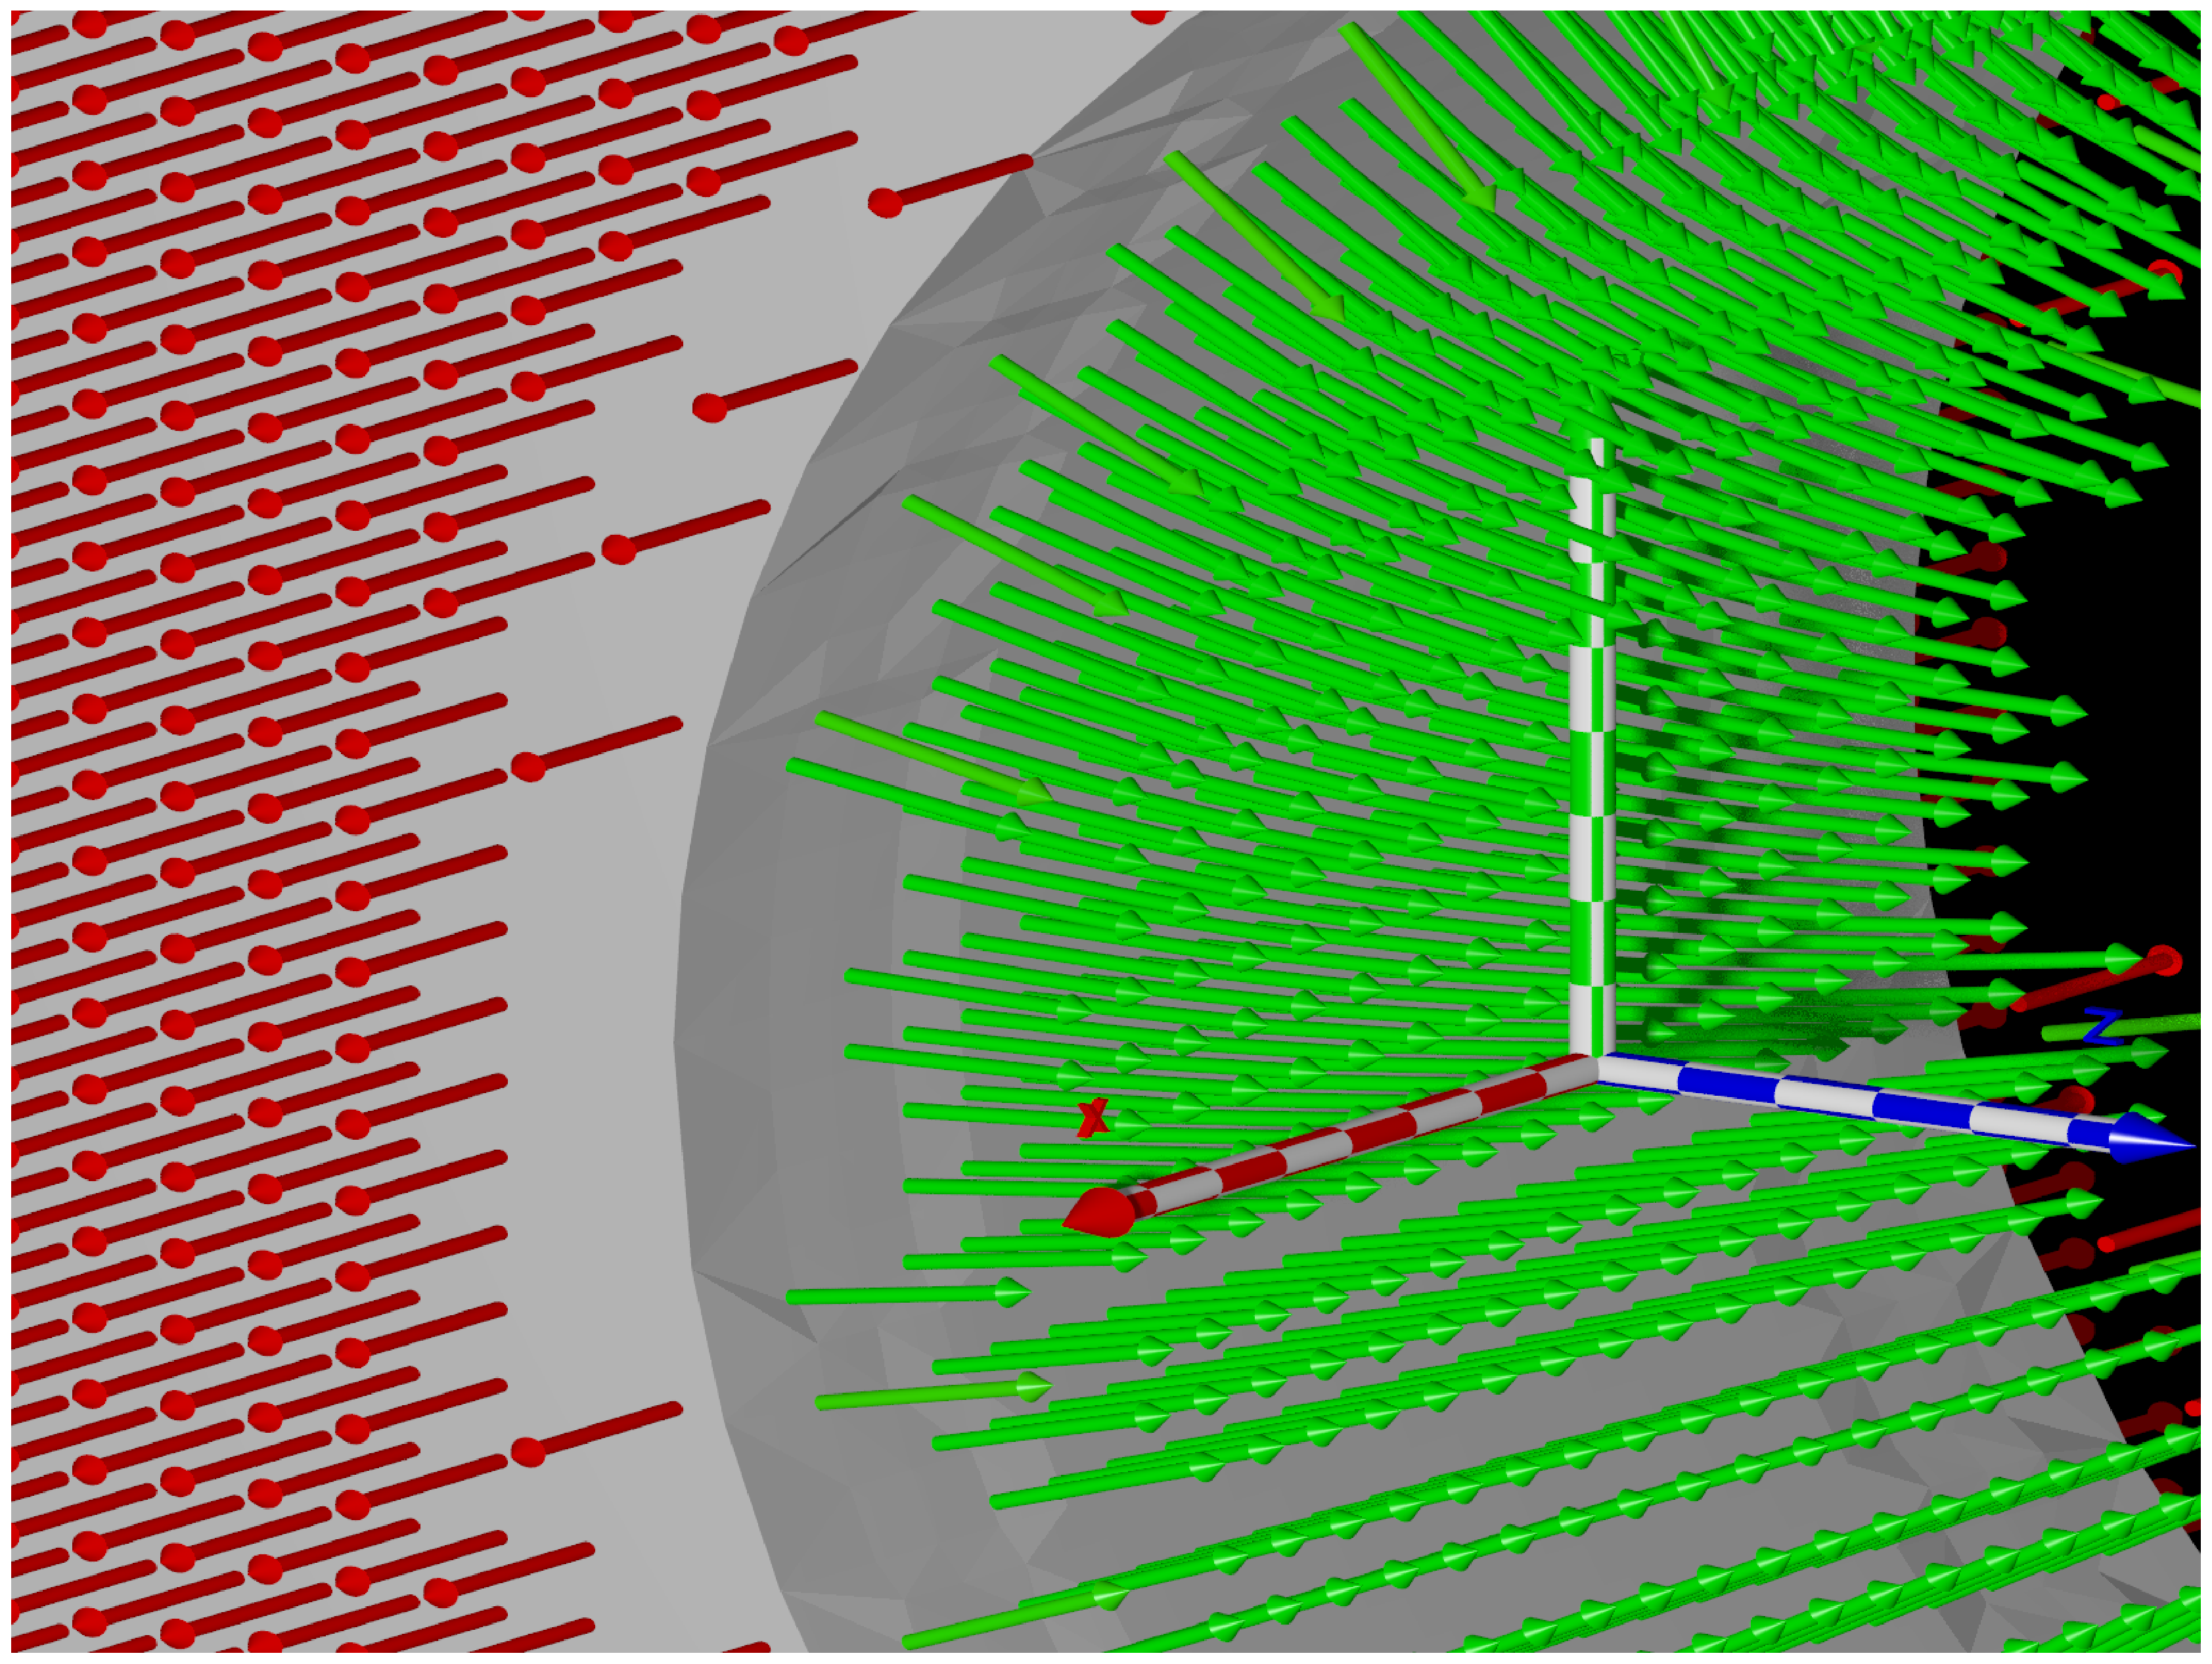
\includegraphics[width=0.33\linewidth]{images/annulus.gradcompare.algo1.eps}\label{fig:annulus:algo1}}
    \subfloat[Edge dist. 2 predictions]{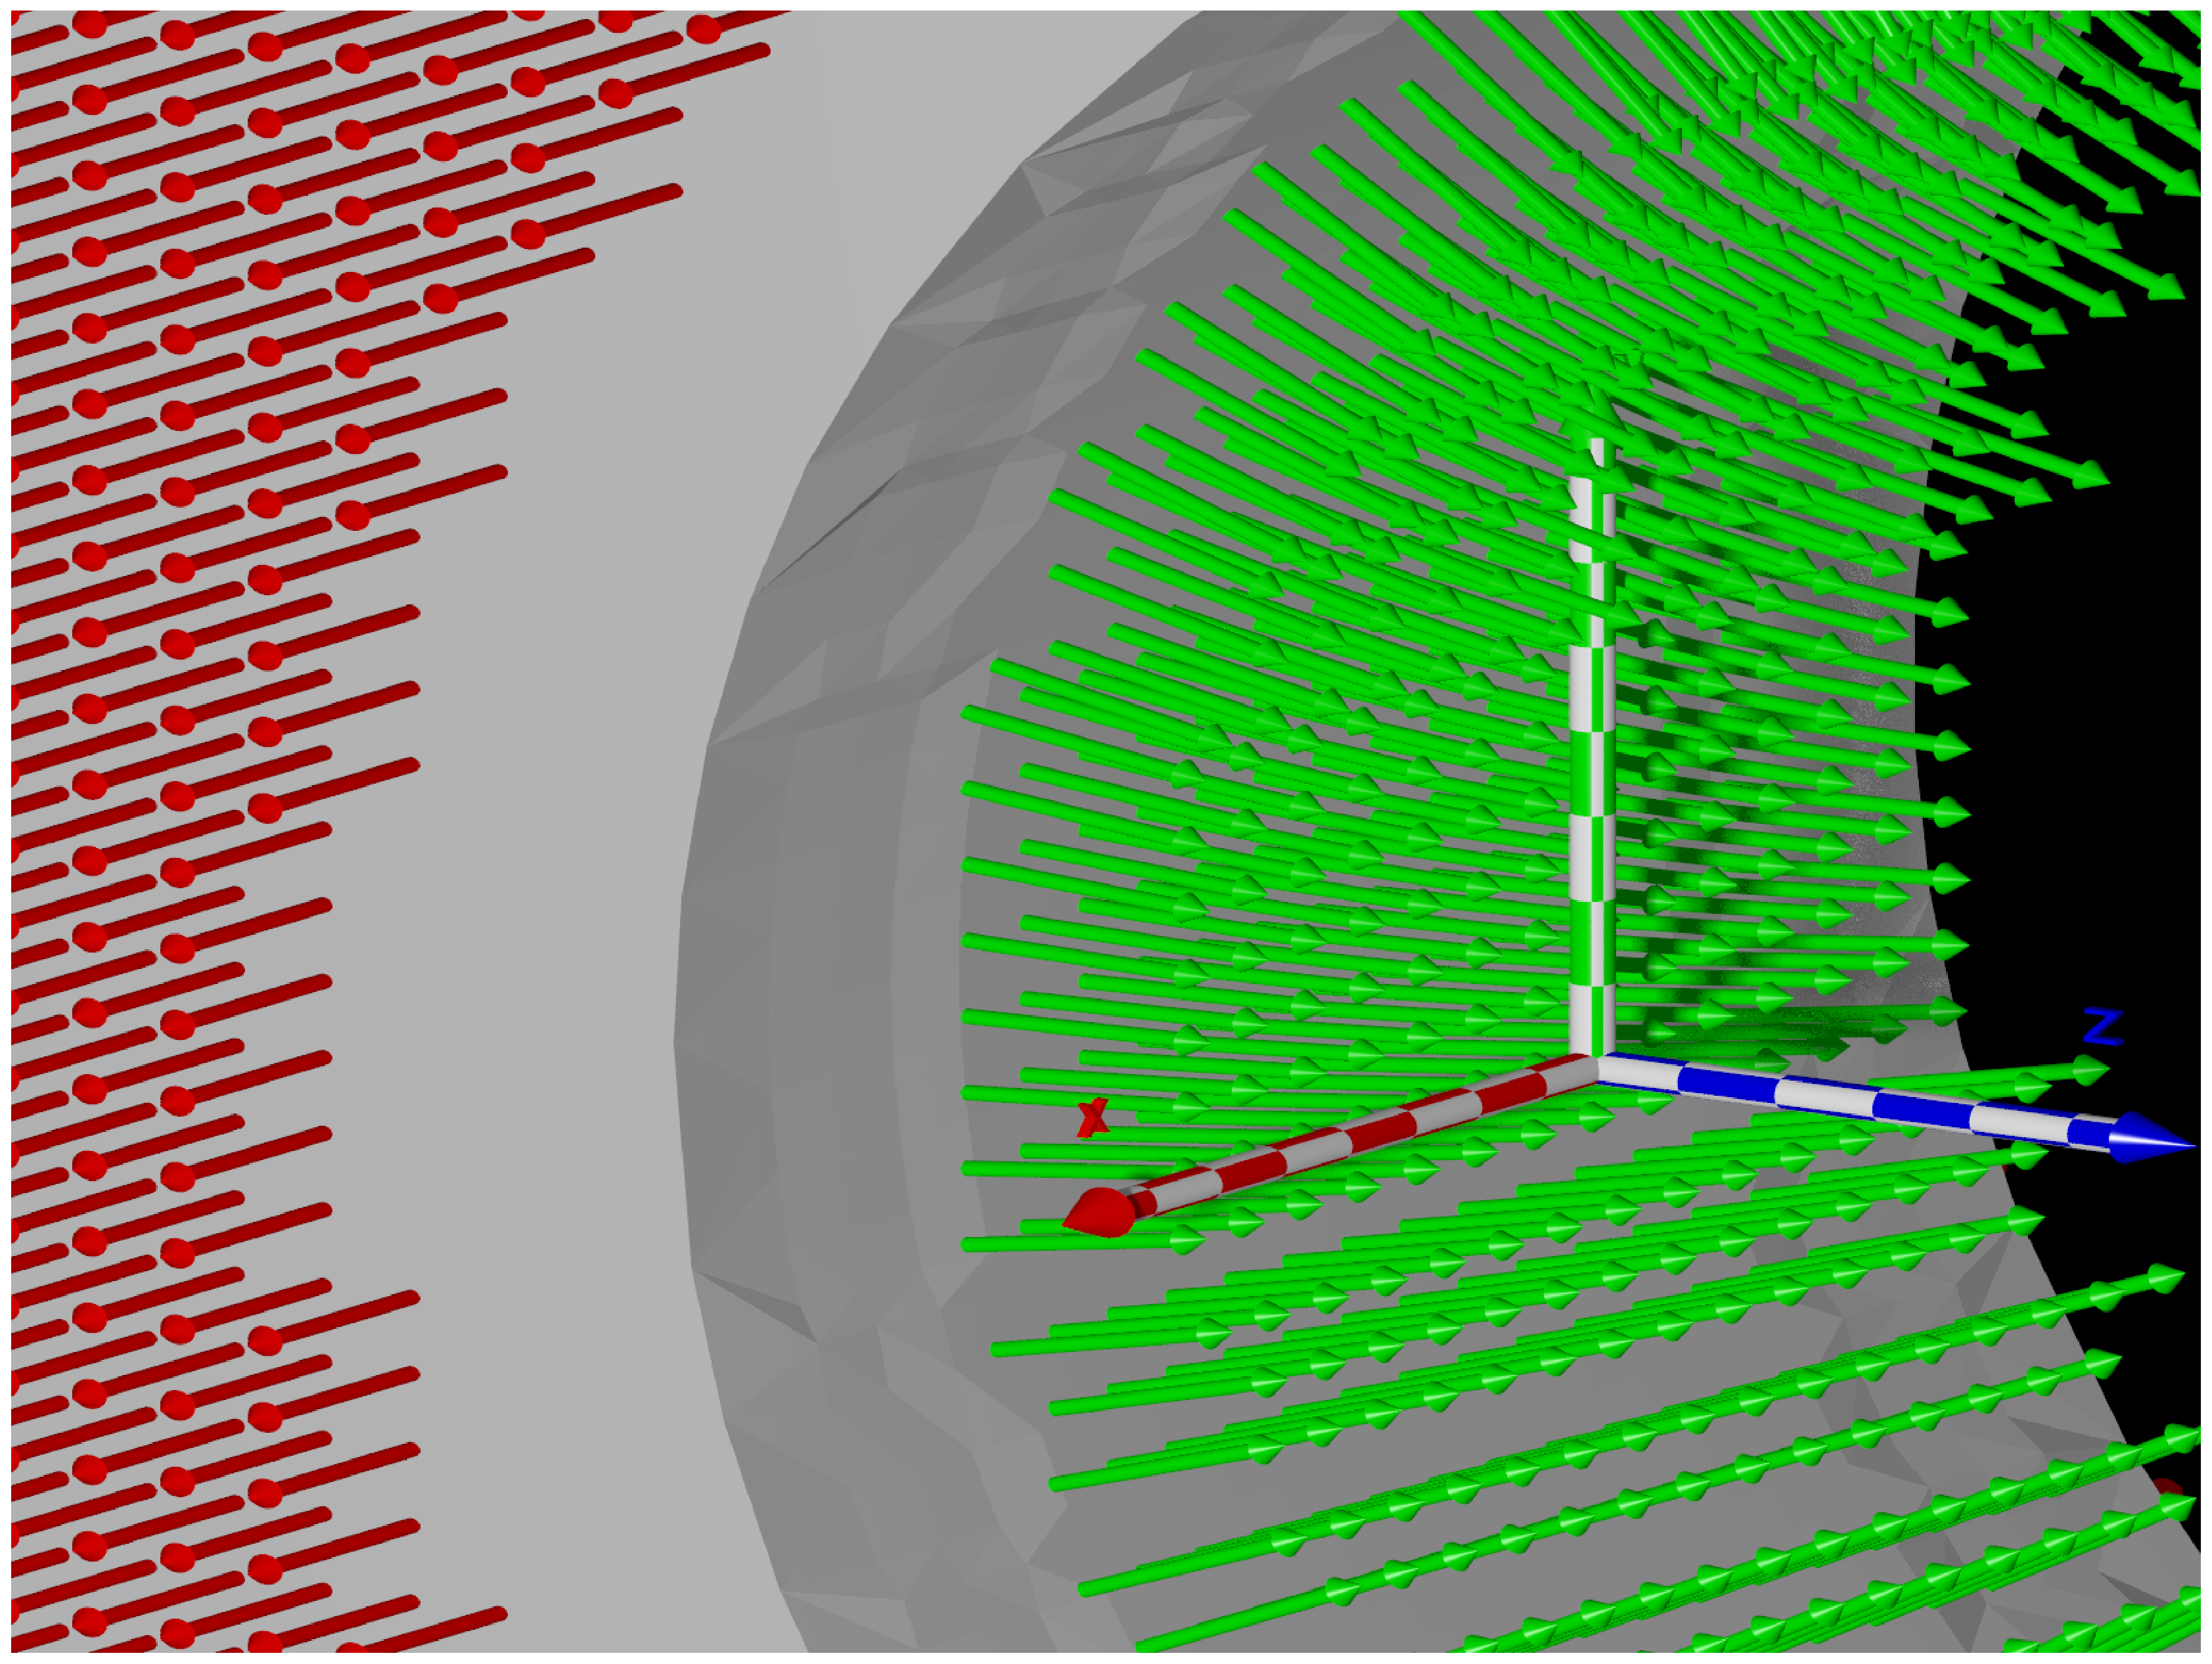
\includegraphics[width=0.33\linewidth]{images/annulus.gradcompare.algo2.eps}\label{fig:annulus:algo2}}\\\vspace{-4mm}
    \subfloat[Central Difference]{\includegraphics[width=0.5\linewidth]{images/gradCompare.full.A.eps}\label{fig:annulus:cdiff} }
    \subfloat[ReliGrad]
    {\includegraphics[width=0.5\linewidth]{images/gradCompare.full.B.eps}\label{fig:annulus:religrad} }\vspace{-3mm}
    \caption{Gradient results on a part of the \emph{Annulus} dataset (Figure~\protect\subref*{fig:annulus}).
        \protect\subref{fig:annulus:correct} Correct gradients.
        \protect\subref{fig:annulus:algo1}  Gradients marked correct by Algorithm 1 which uses $n_{v''}$ and $n_{v'}$ to predict $n_v$.
        \protect\subref{fig:annulus:algo2} Gradients marked correct by Algorithm 2 which uses $n_{v'''}$, $n_{v''}$, and $n_{v'}$ to predict $n_v$.
        \protect\subref{fig:annulus:cdiff} Central difference gradients. The blue inset on the right contains a magnified view. 
        \protect\subref{fig:annulus:religrad} Gradients marked correct by \protect\ReliGrad. The cyan inset shows a magnified view.
    }    
    \label{fig:annulus:gradResults}
\end{figure}
\textbf{Reliable Gradients:}
Figure~\ref{fig:annulus:gradResults} shows gradients at grid vertices for grid cubes which intersect the isosurface on a zoomed in section of the \textit{Annulus} dataset.
To get the colormap for the gradient vectors, we projected all gradient vectors on to the XY plane, the angle of the resulting vector to the X-Axis is mapped between red-green. Gradients close to X-Axis are red, those perpendicular are green. 
Figure~\protect\subref*{fig:annulus:correct} shows the known correct gradients at all the grid vertices.  Figure~\subref*{fig:annulus:cdiff}, shows the central difference (CDiff) gradients at all the grid vertices. The blue inset shows a magnified view: CDiff gradients are inaccurate along discontinuities.
Figure~\subref*{fig:annulus:algo1} shows gradients only at vertices marked correct by Algorithm 1,  which uses $n_{v''}$ and $n_{v'}$ to predict $n_v$. Figure~\protect\subref*{fig:annulus:algo2} shows results from Algorithm 2, which uses $n_{v'''}$, $n_{v''}$, and $n_{v'}$ to predict $n_v$. 
Figure~\subref*{fig:annulus:religrad} shows gradients marked reliable by \protect\ReliGrad, the cyan inset shows a close-up, the inaccurate gradients are marked unreliable  by \ReliGrad and not shown. 

% %Cannon
\begin{figure}
    \centering
    \subfloat[Correct ]{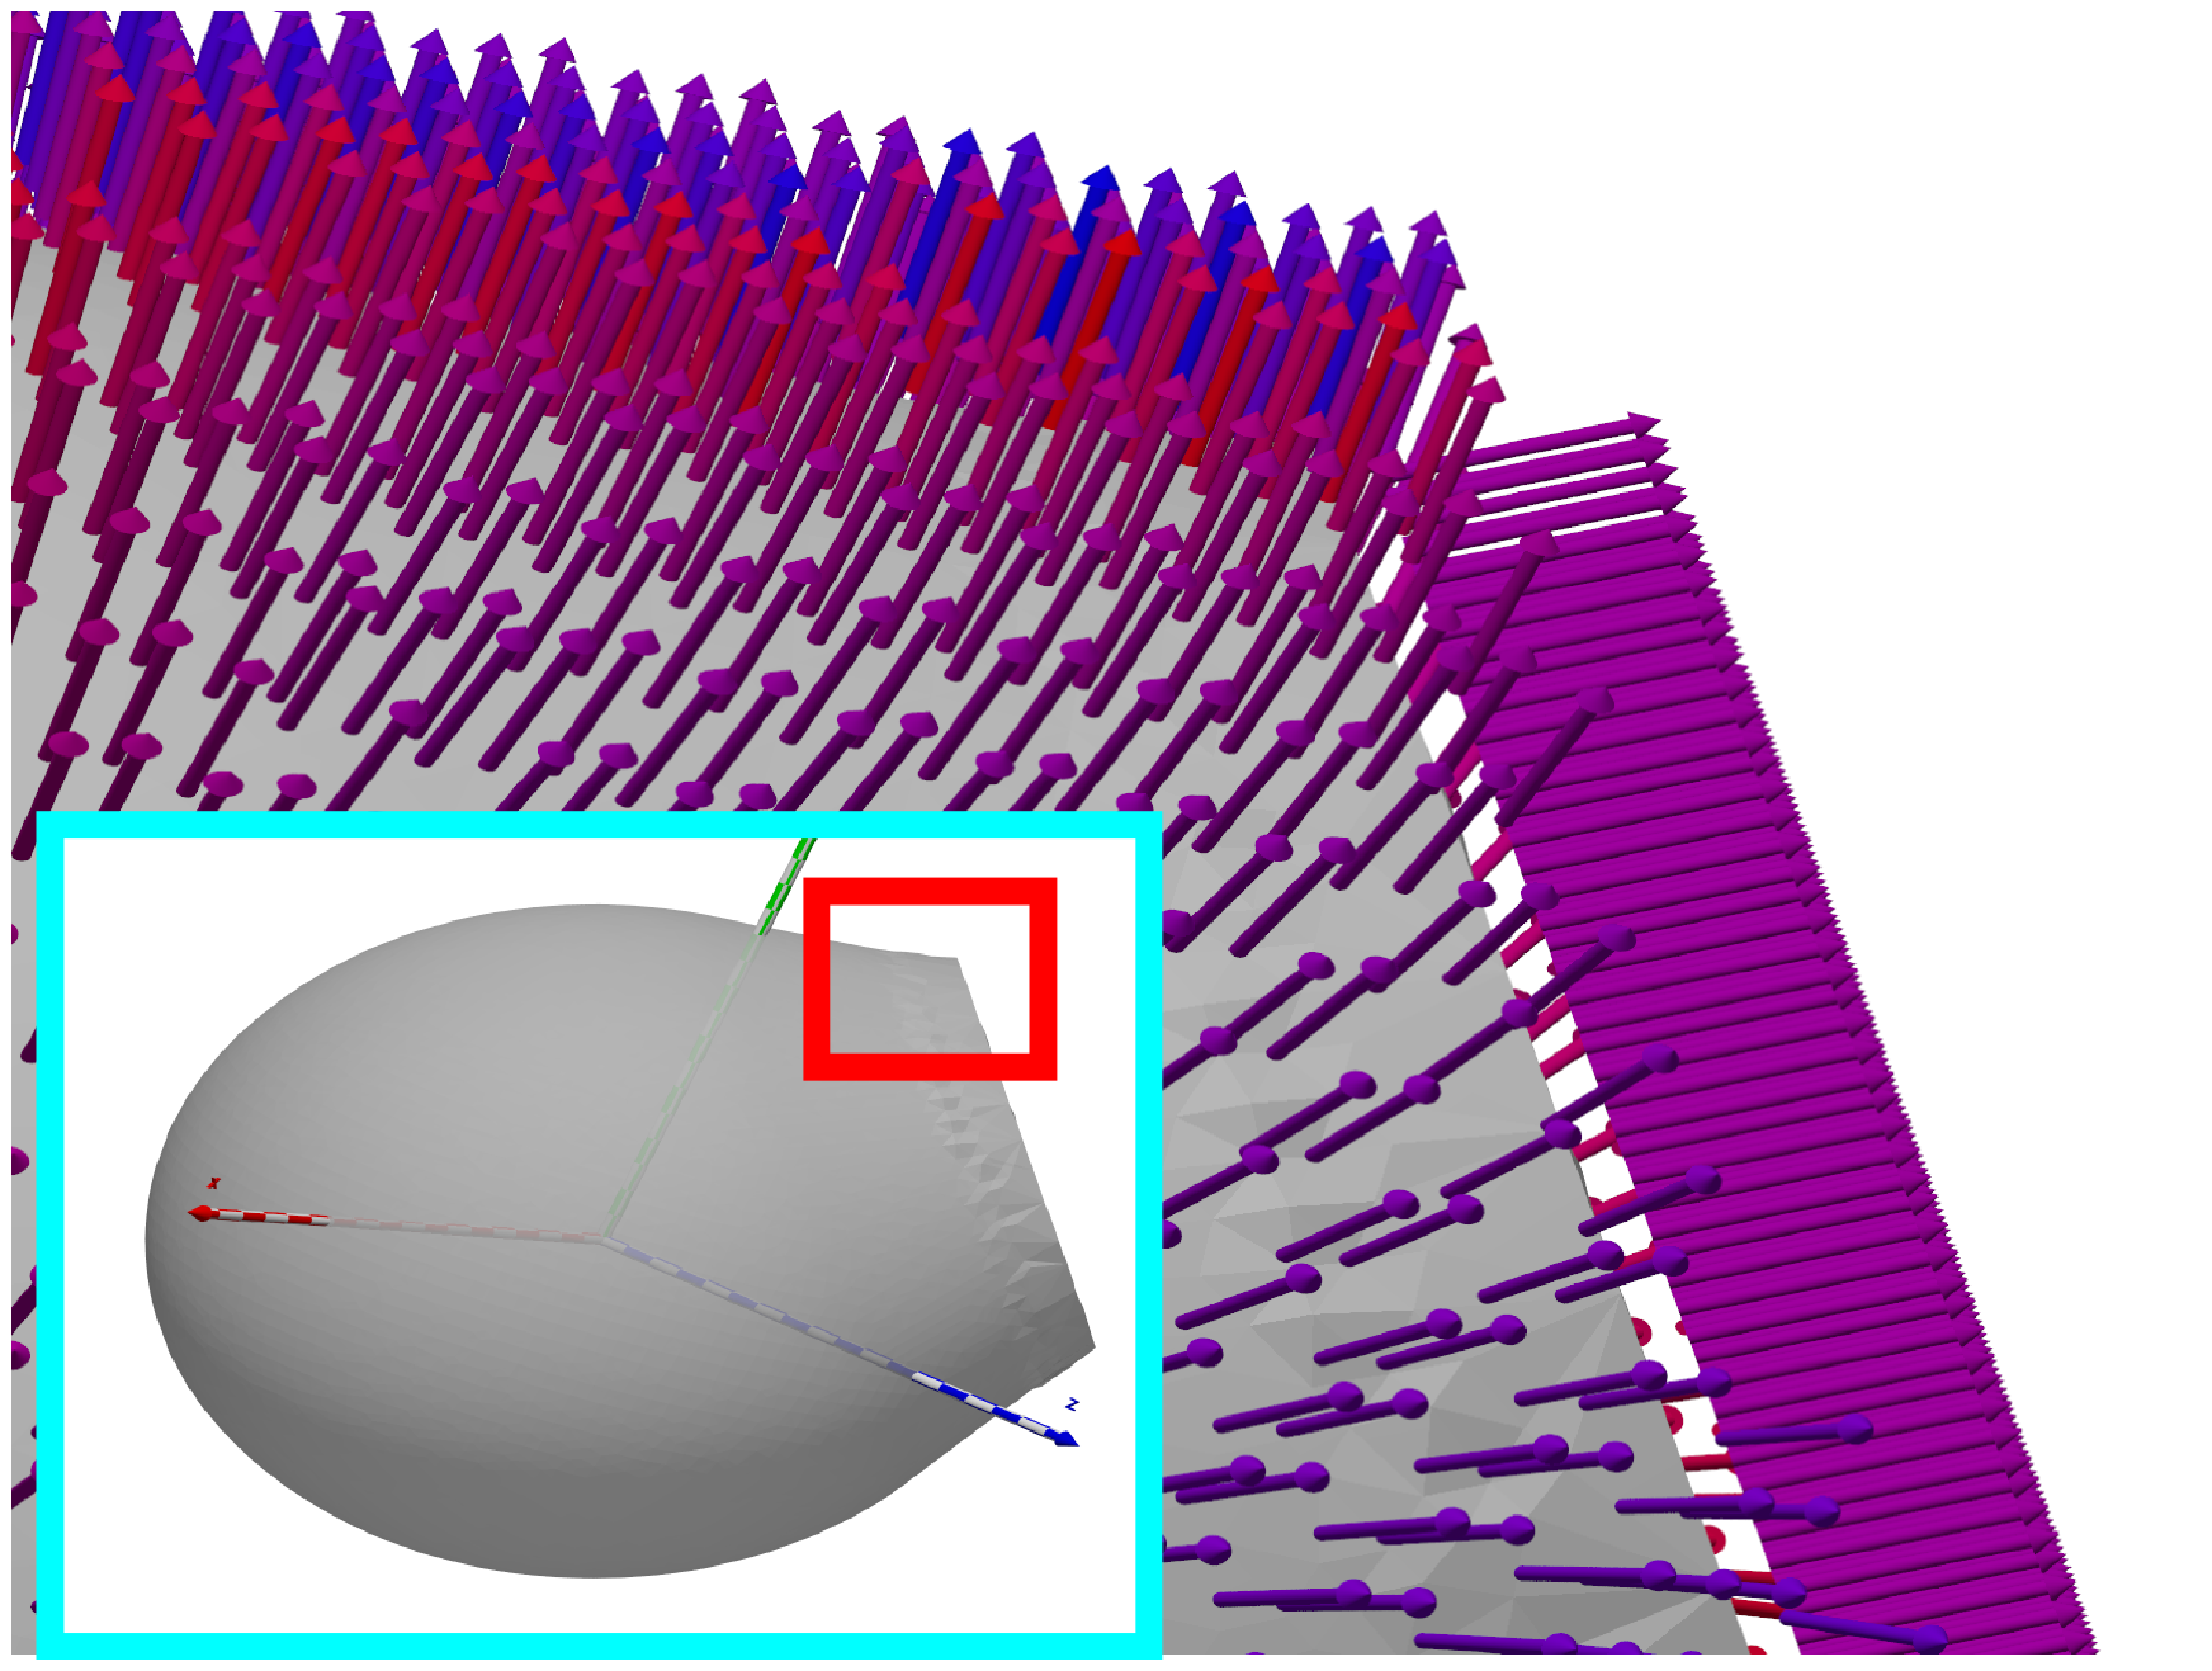
\includegraphics[width=0.25\linewidth]
        {images/cannon.correct.close.eps}\label{fig:cannon.correct}}
    \subfloat[CDiff]{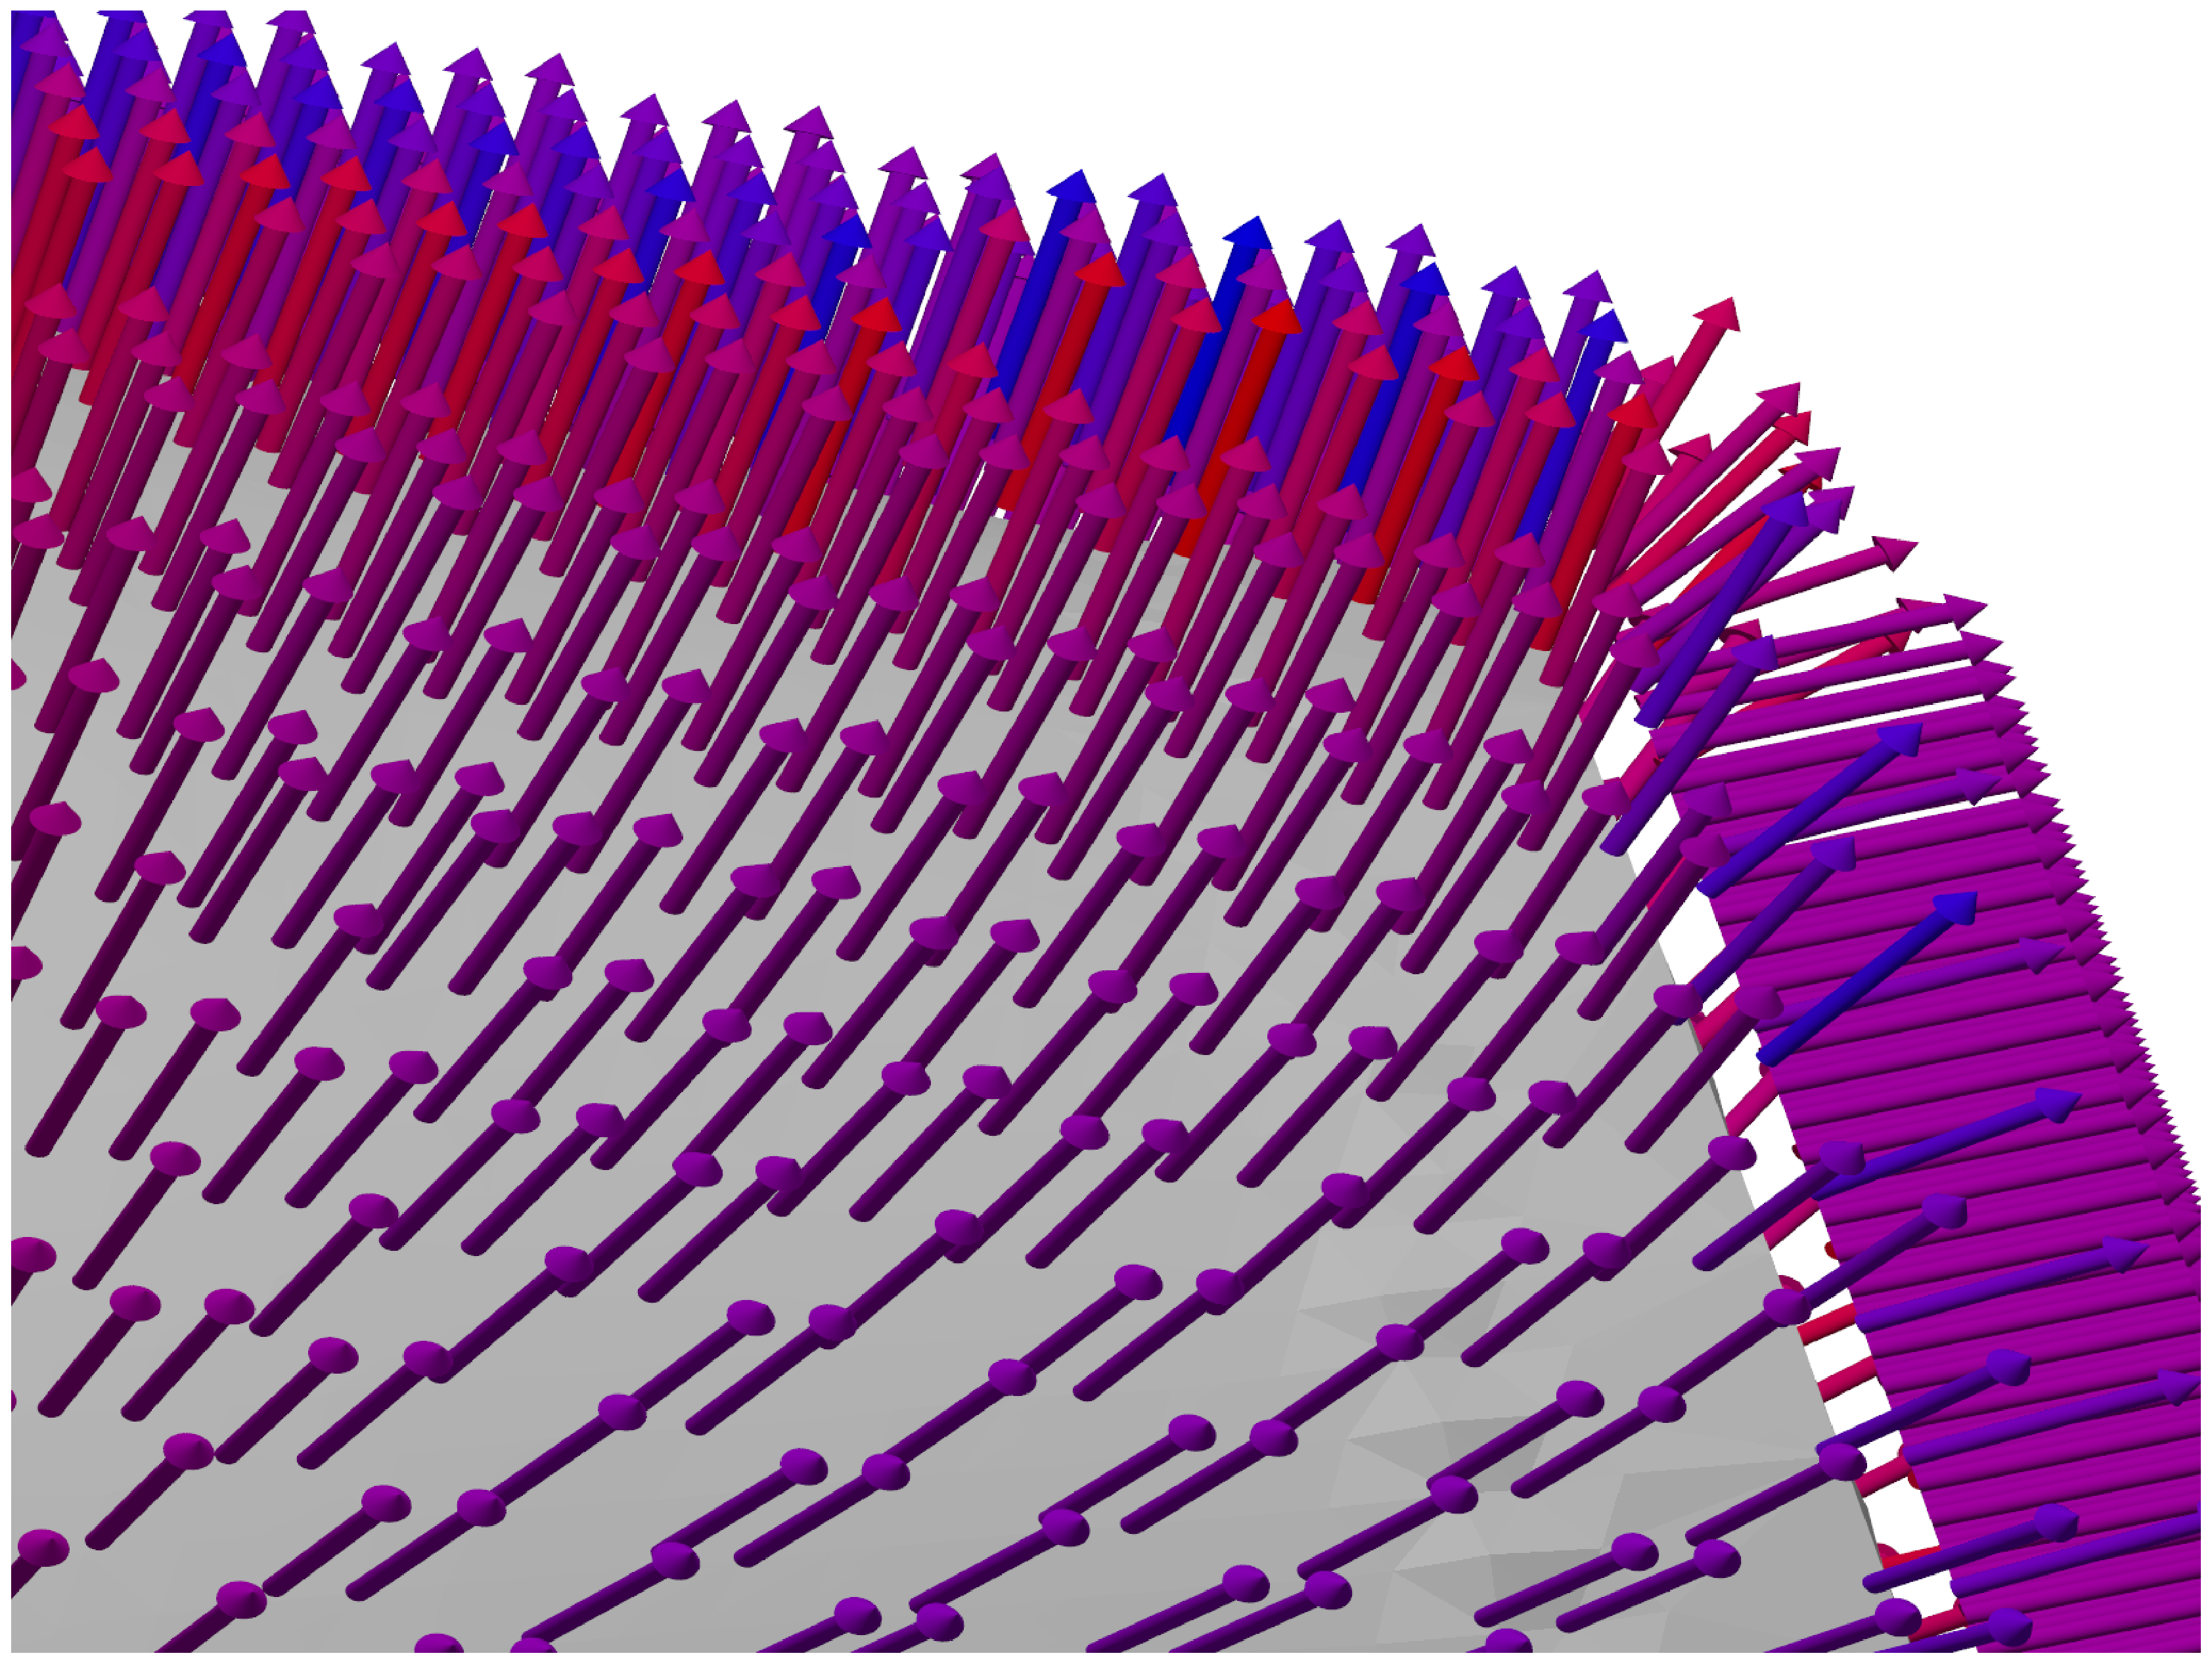
\includegraphics[width=0.25\linewidth]
        {images/cannon.cdiff.close.eps}\label{fig:cannon.cdiff}}  
    \subfloat[FindReliable]{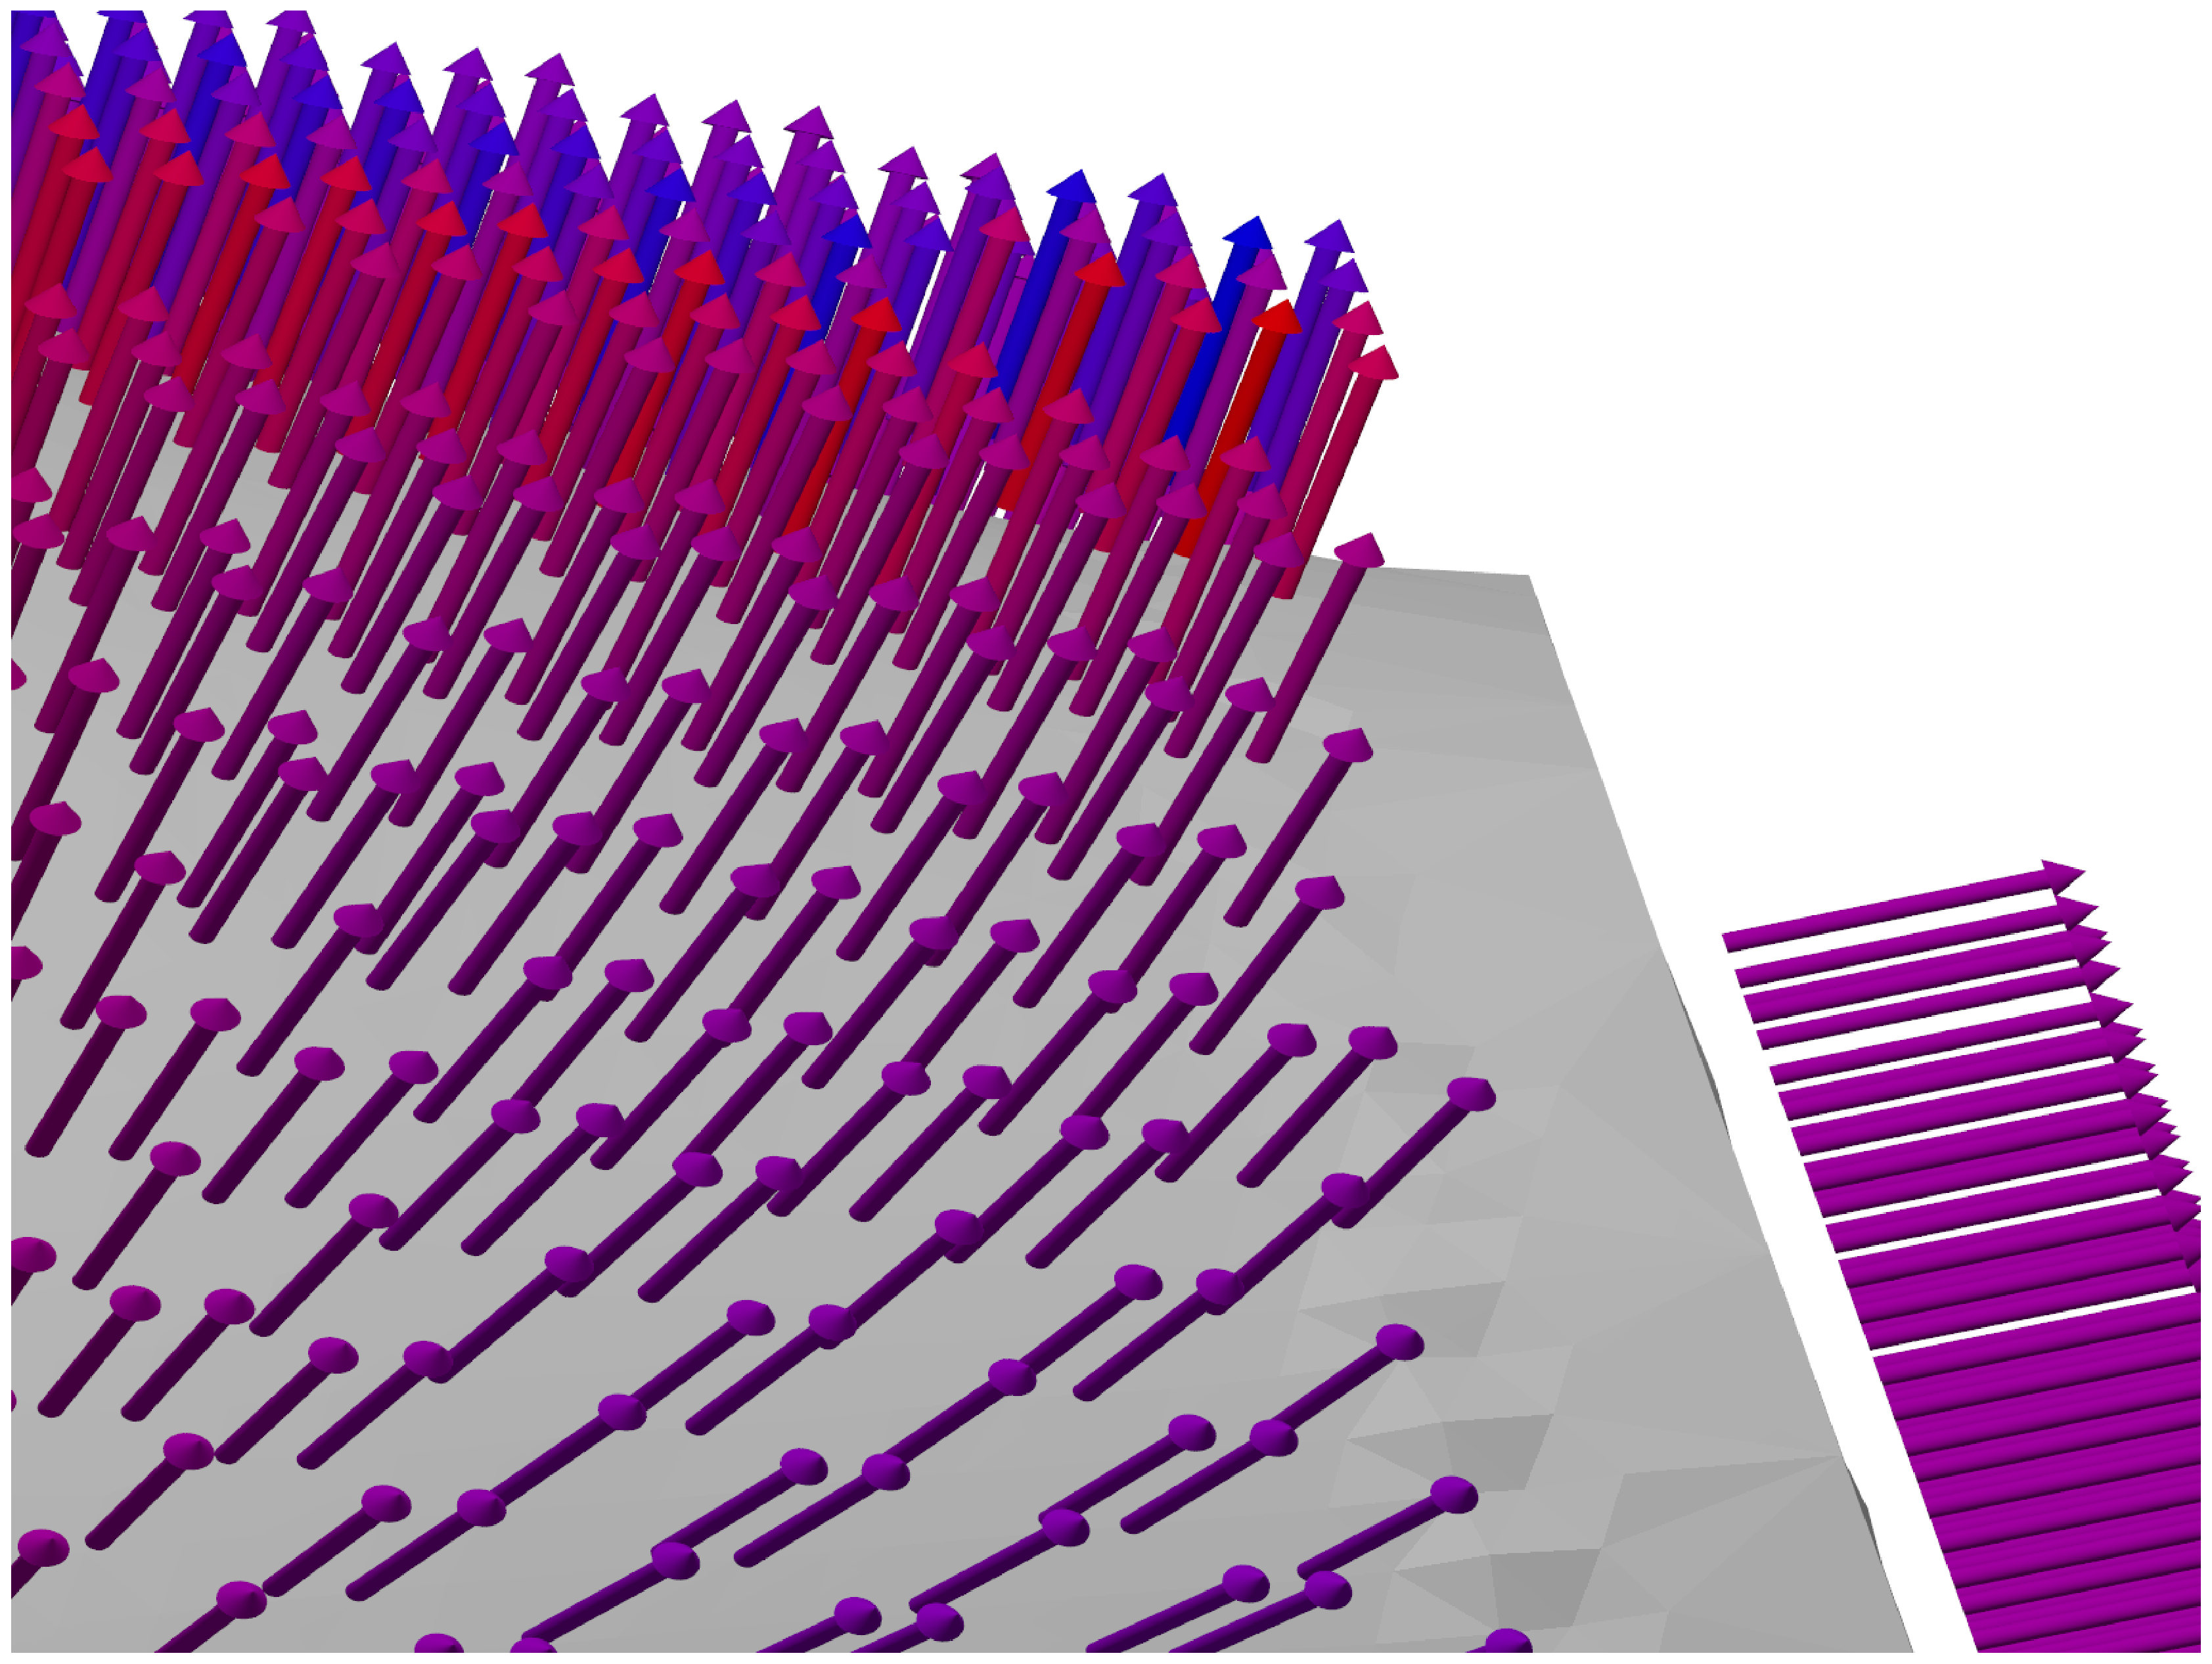
\includegraphics[width=0.25\linewidth]
        {images/cannon.findreliable.close.eps}\label{fig:cannon.findreliable}}
    \subfloat[Religrad]{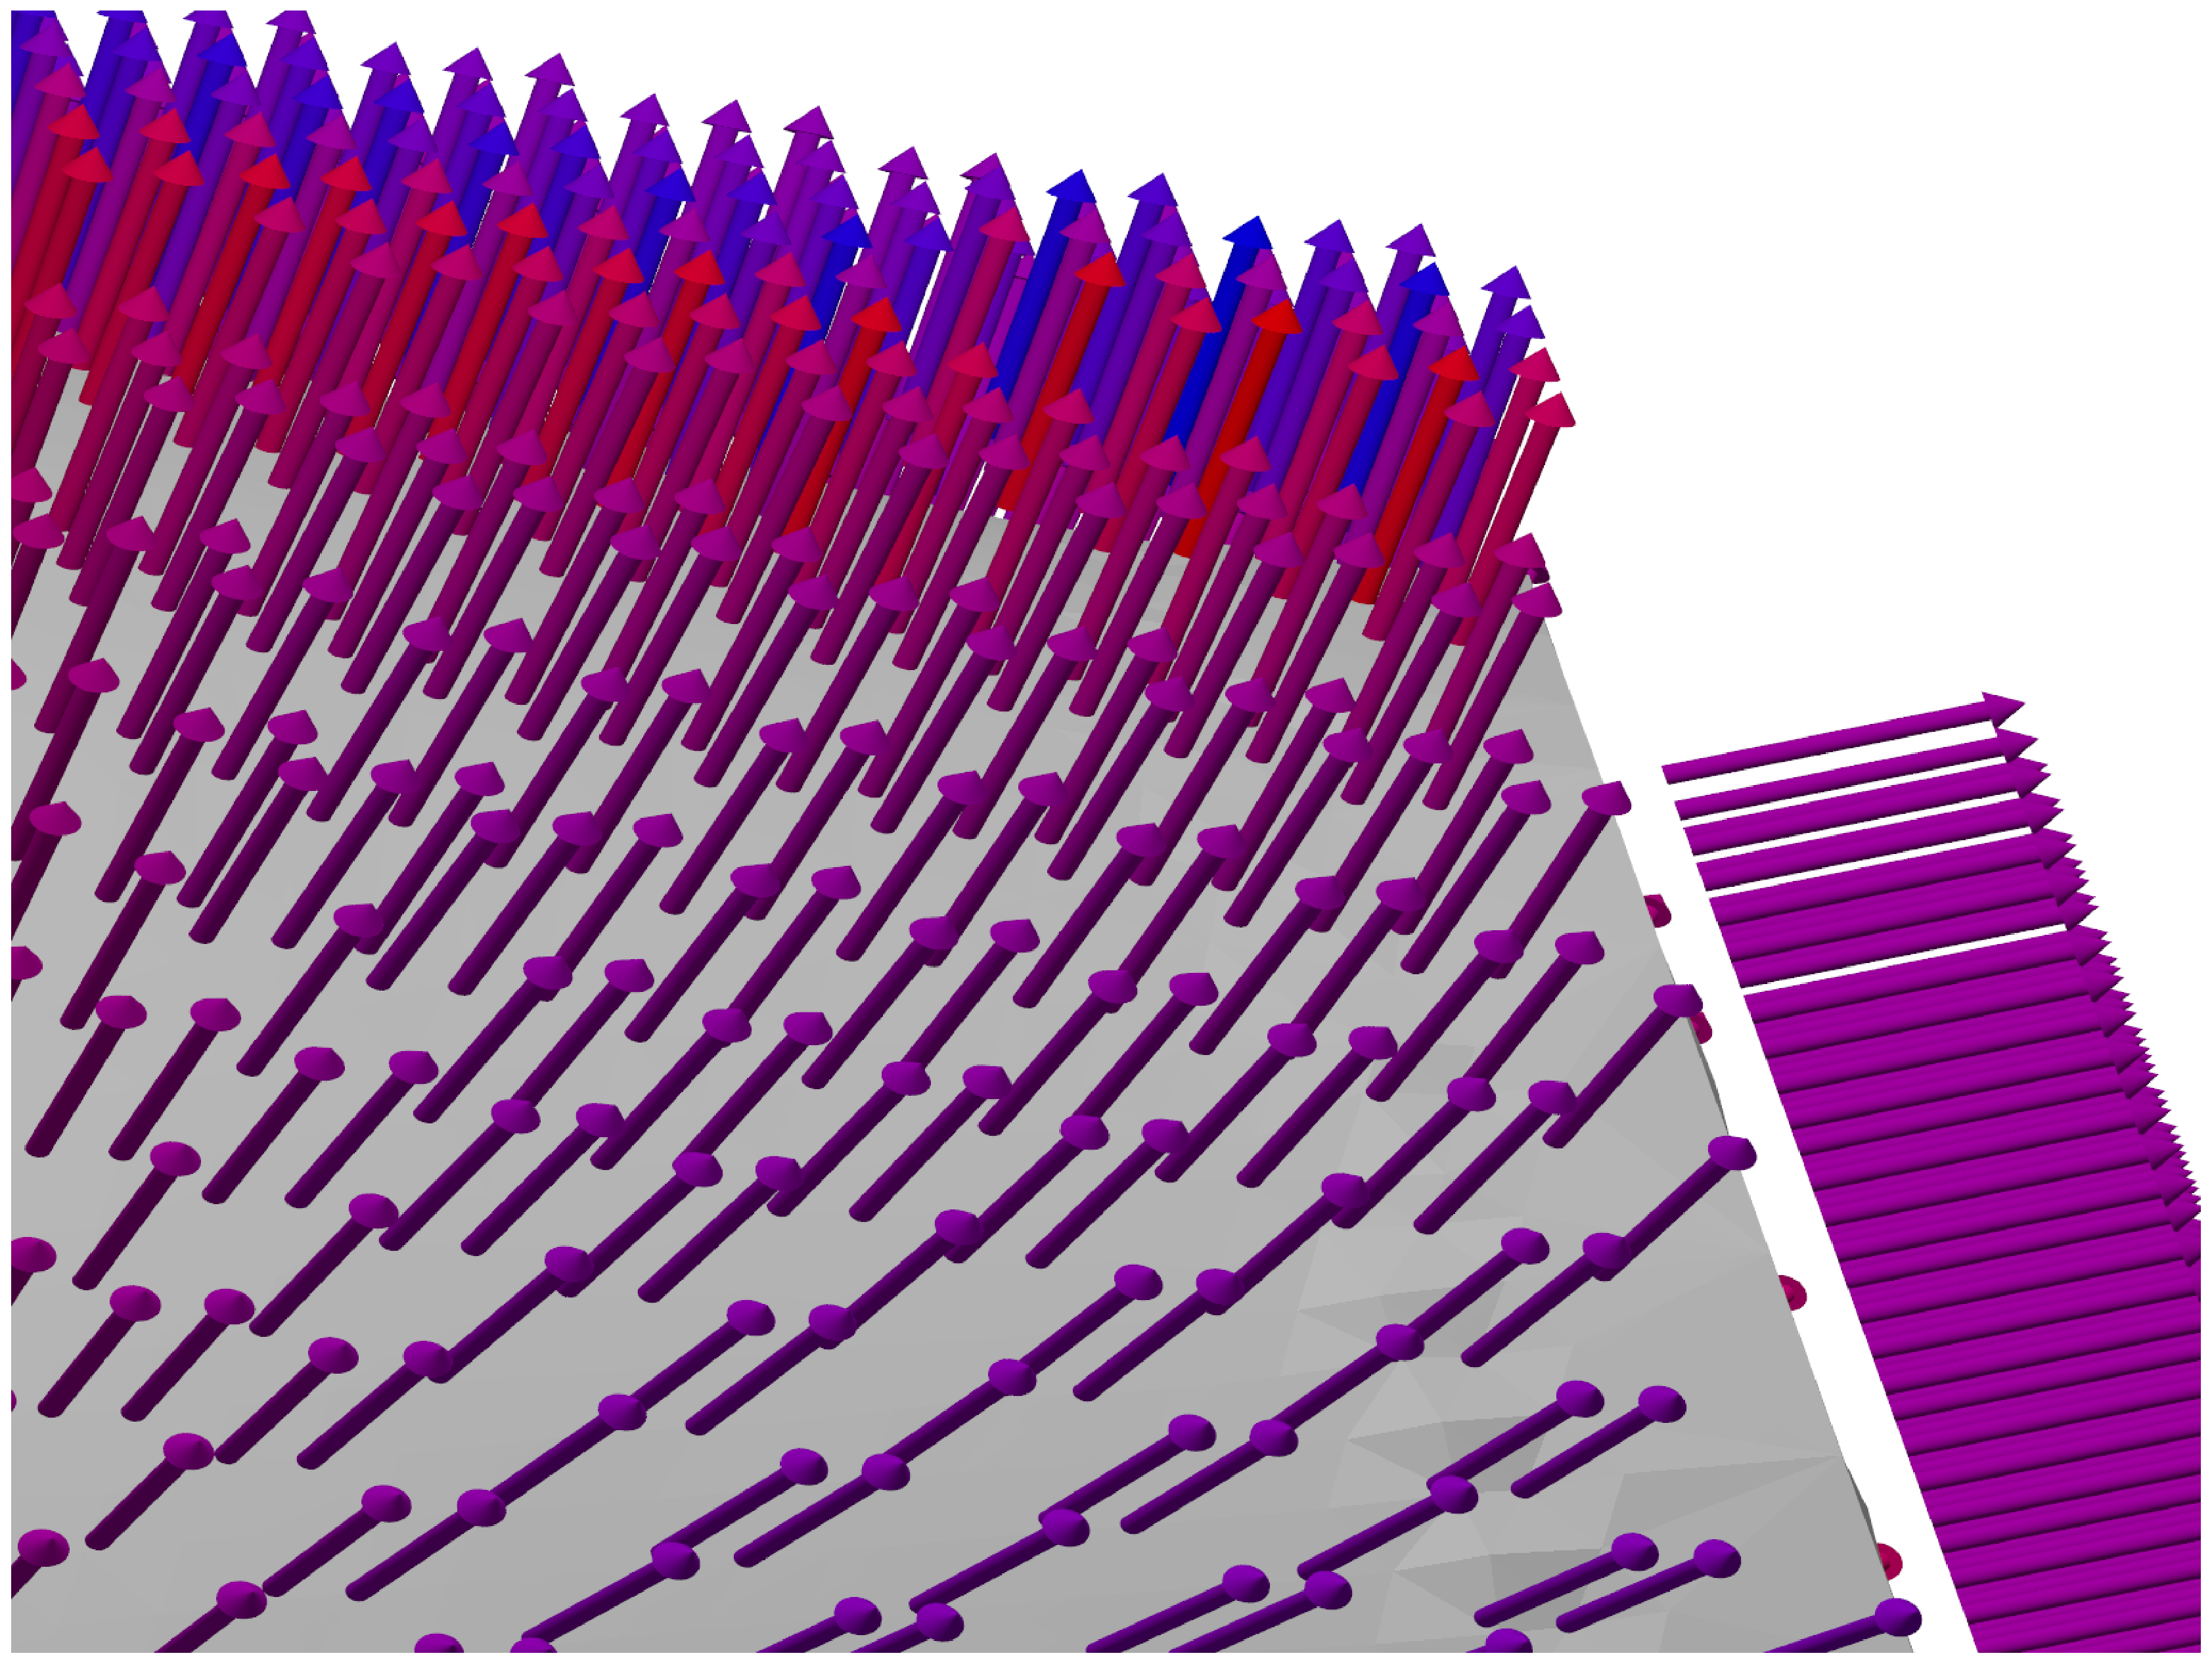
\includegraphics[width=0.25\linewidth]
        {images/cannon.religrad.close.eps}\label{fig:cannon.religrad}}\vspace{-3mm}
    \caption{Cannon dataset gradients (Curved edge, non 90$^\circ$ angles). \protect\subref{fig:cannon.correct} correct gradients, \protect\subref{fig:cannon.cdiff} central difference gradients, \protect\subref{fig:cannon.findreliable} gradients marked correct by FindReliable. \protect\subref{fig:cannon.religrad}  gradients at grid vertices marked correct by \protect\ReliGrad. Inaccurate CDiff gradients Figure\protect\subref{fig:cannon.cdiff} across the discontinuity are not marked correct, hence not shown.}
    \label{fig:cannon:gradients}
\end{figure}


%\begin{figure*}
%    \centering
%    \subfloat[Correct gradients]{\includegraphics[width=0.25\linewidth]
%        {images/cannon.correct.close.eps}\label{fig:cannon.correct}}
%    \subfloat[CDiff gradients]{\includegraphics[width=0.24\linewidth]
%        {images/cannon.cdiff.close.eps}\label{fig:cannon.cdiff}}\hspace{1mm}     
%    \subfloat[FindReliable gradients]{\includegraphics[width=0.24\linewidth]
%        {images/cannon.findreliable.close.eps}\label{fig:cannon.findreliable}}
%      \hspace{1mm}  
%    \subfloat[Religrad gradients]{\includegraphics[width=0.24\linewidth]
%        {images/cannon.religrad.close.eps}\label{fig:cannon.religrad}}
%    \caption{Cannon dataset gradients (Curved edge, non 90$^\circ$ angles). \protect\subref{fig:cannon.correct} correct gradients, \protect\subref{fig:cannon.cdiff} central difference gradients, \protect\subref{fig:cannon.findreliable} gradients marked correct by FindReliable. \protect\subref{fig:cannon.religrad}  gradients at grid vertices marked correct by \protect\ReliGrad. Inaccurate CDiff gradients \protect\subref{fig:cannon.cdiff} across the discontinuity are not marked correct, hence not shown.}
%    \label{fig:cannon:gradients}
%\end{figure*}
Figure~\ref{fig:cannon:gradients} shows the gradients around the edge of the \textit{Cannon} dataset (Figure~\subref*{fig:cannon.correct} red rectangle shows the location). The dataset is not axis-parallel, the dihedral angle around the curved edge is $120^\circ$. Figure~\subref*{fig:cannon.correct} shows known correct gradients at grid vertices which are intersected by the isosurface. Figure~\subref*{fig:cannon.cdiff} shows the central difference  gradients, at grid vertices of the intersected cubes. Note that along the discontinuity the central difference gradients are inaccurate compared to the correct gradients (Figure~\subref*{fig:cannon.correct}). Figure~\subref*{fig:cannon.findreliable} shows gradients at grid vertices marked reliable by \FindReliable. Figure~\subref*{fig:cannon.religrad} shows gradients marked correct by \ReliGrad.
\begin{figure}[tb]
    \centering
    \subfloat[]{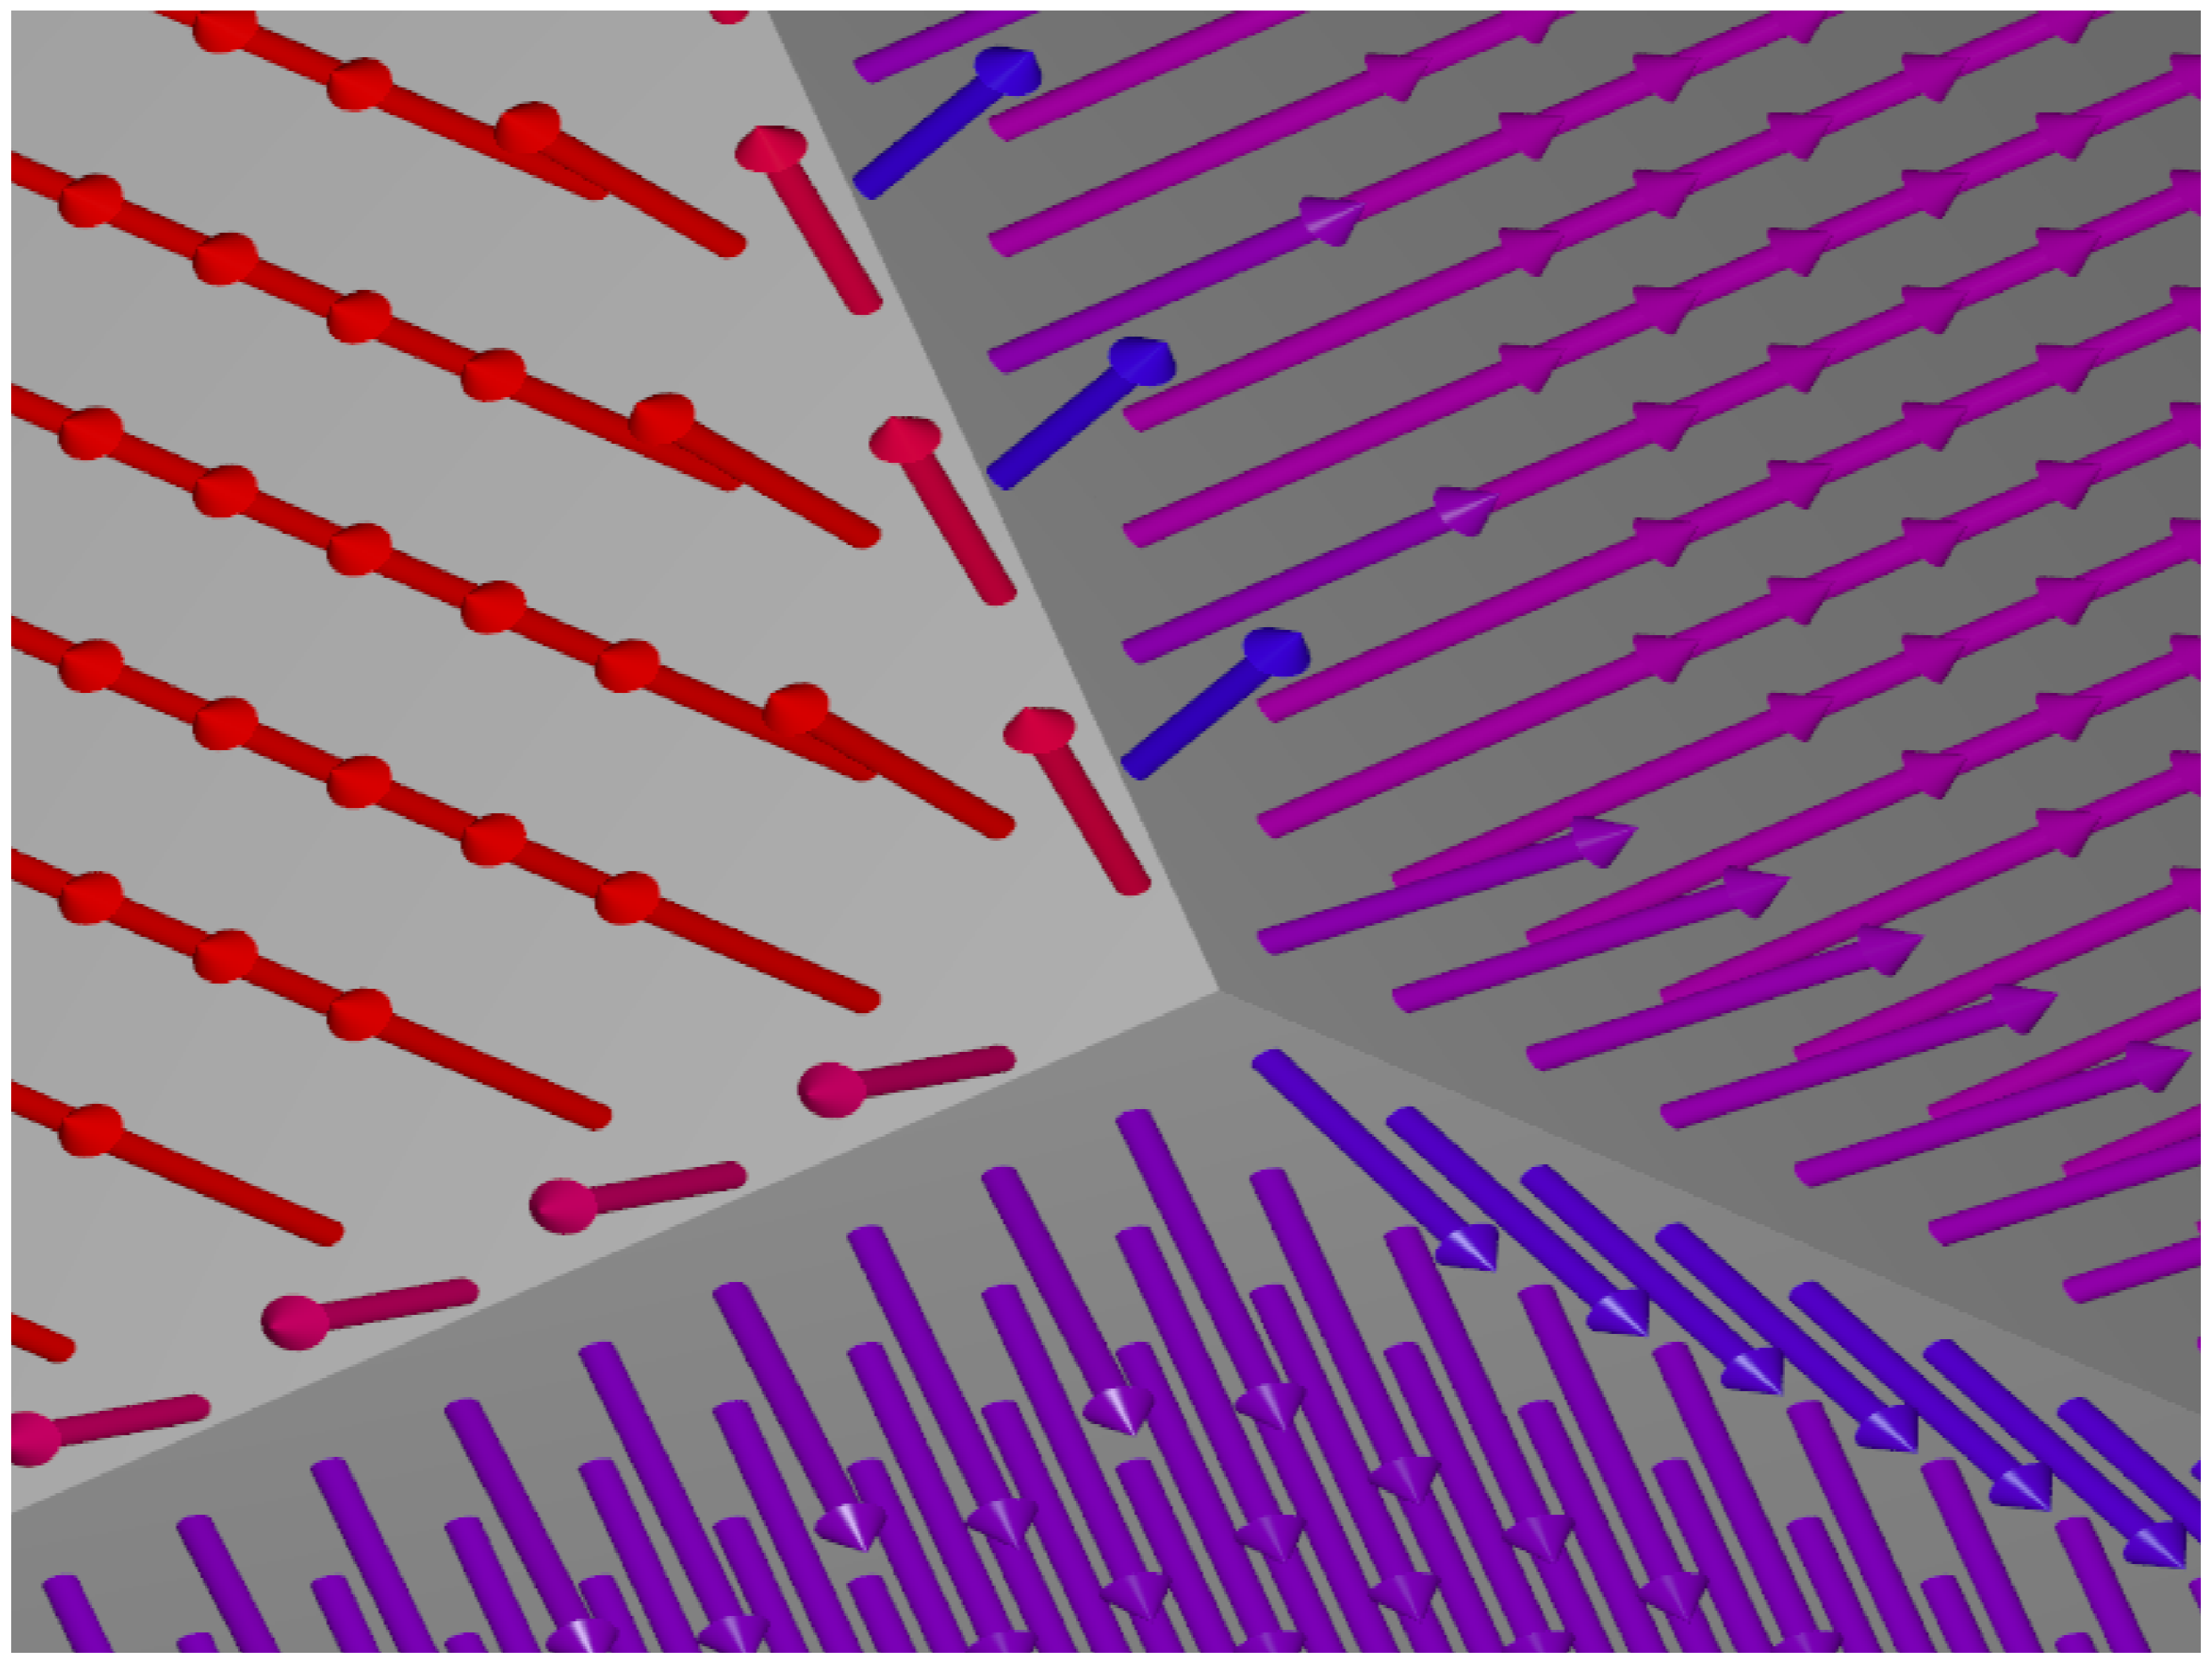
\includegraphics[width=0.25\linewidth]{images/cube.cdiff.eps}\label{fig:cube:cdiff}}
    \subfloat[]{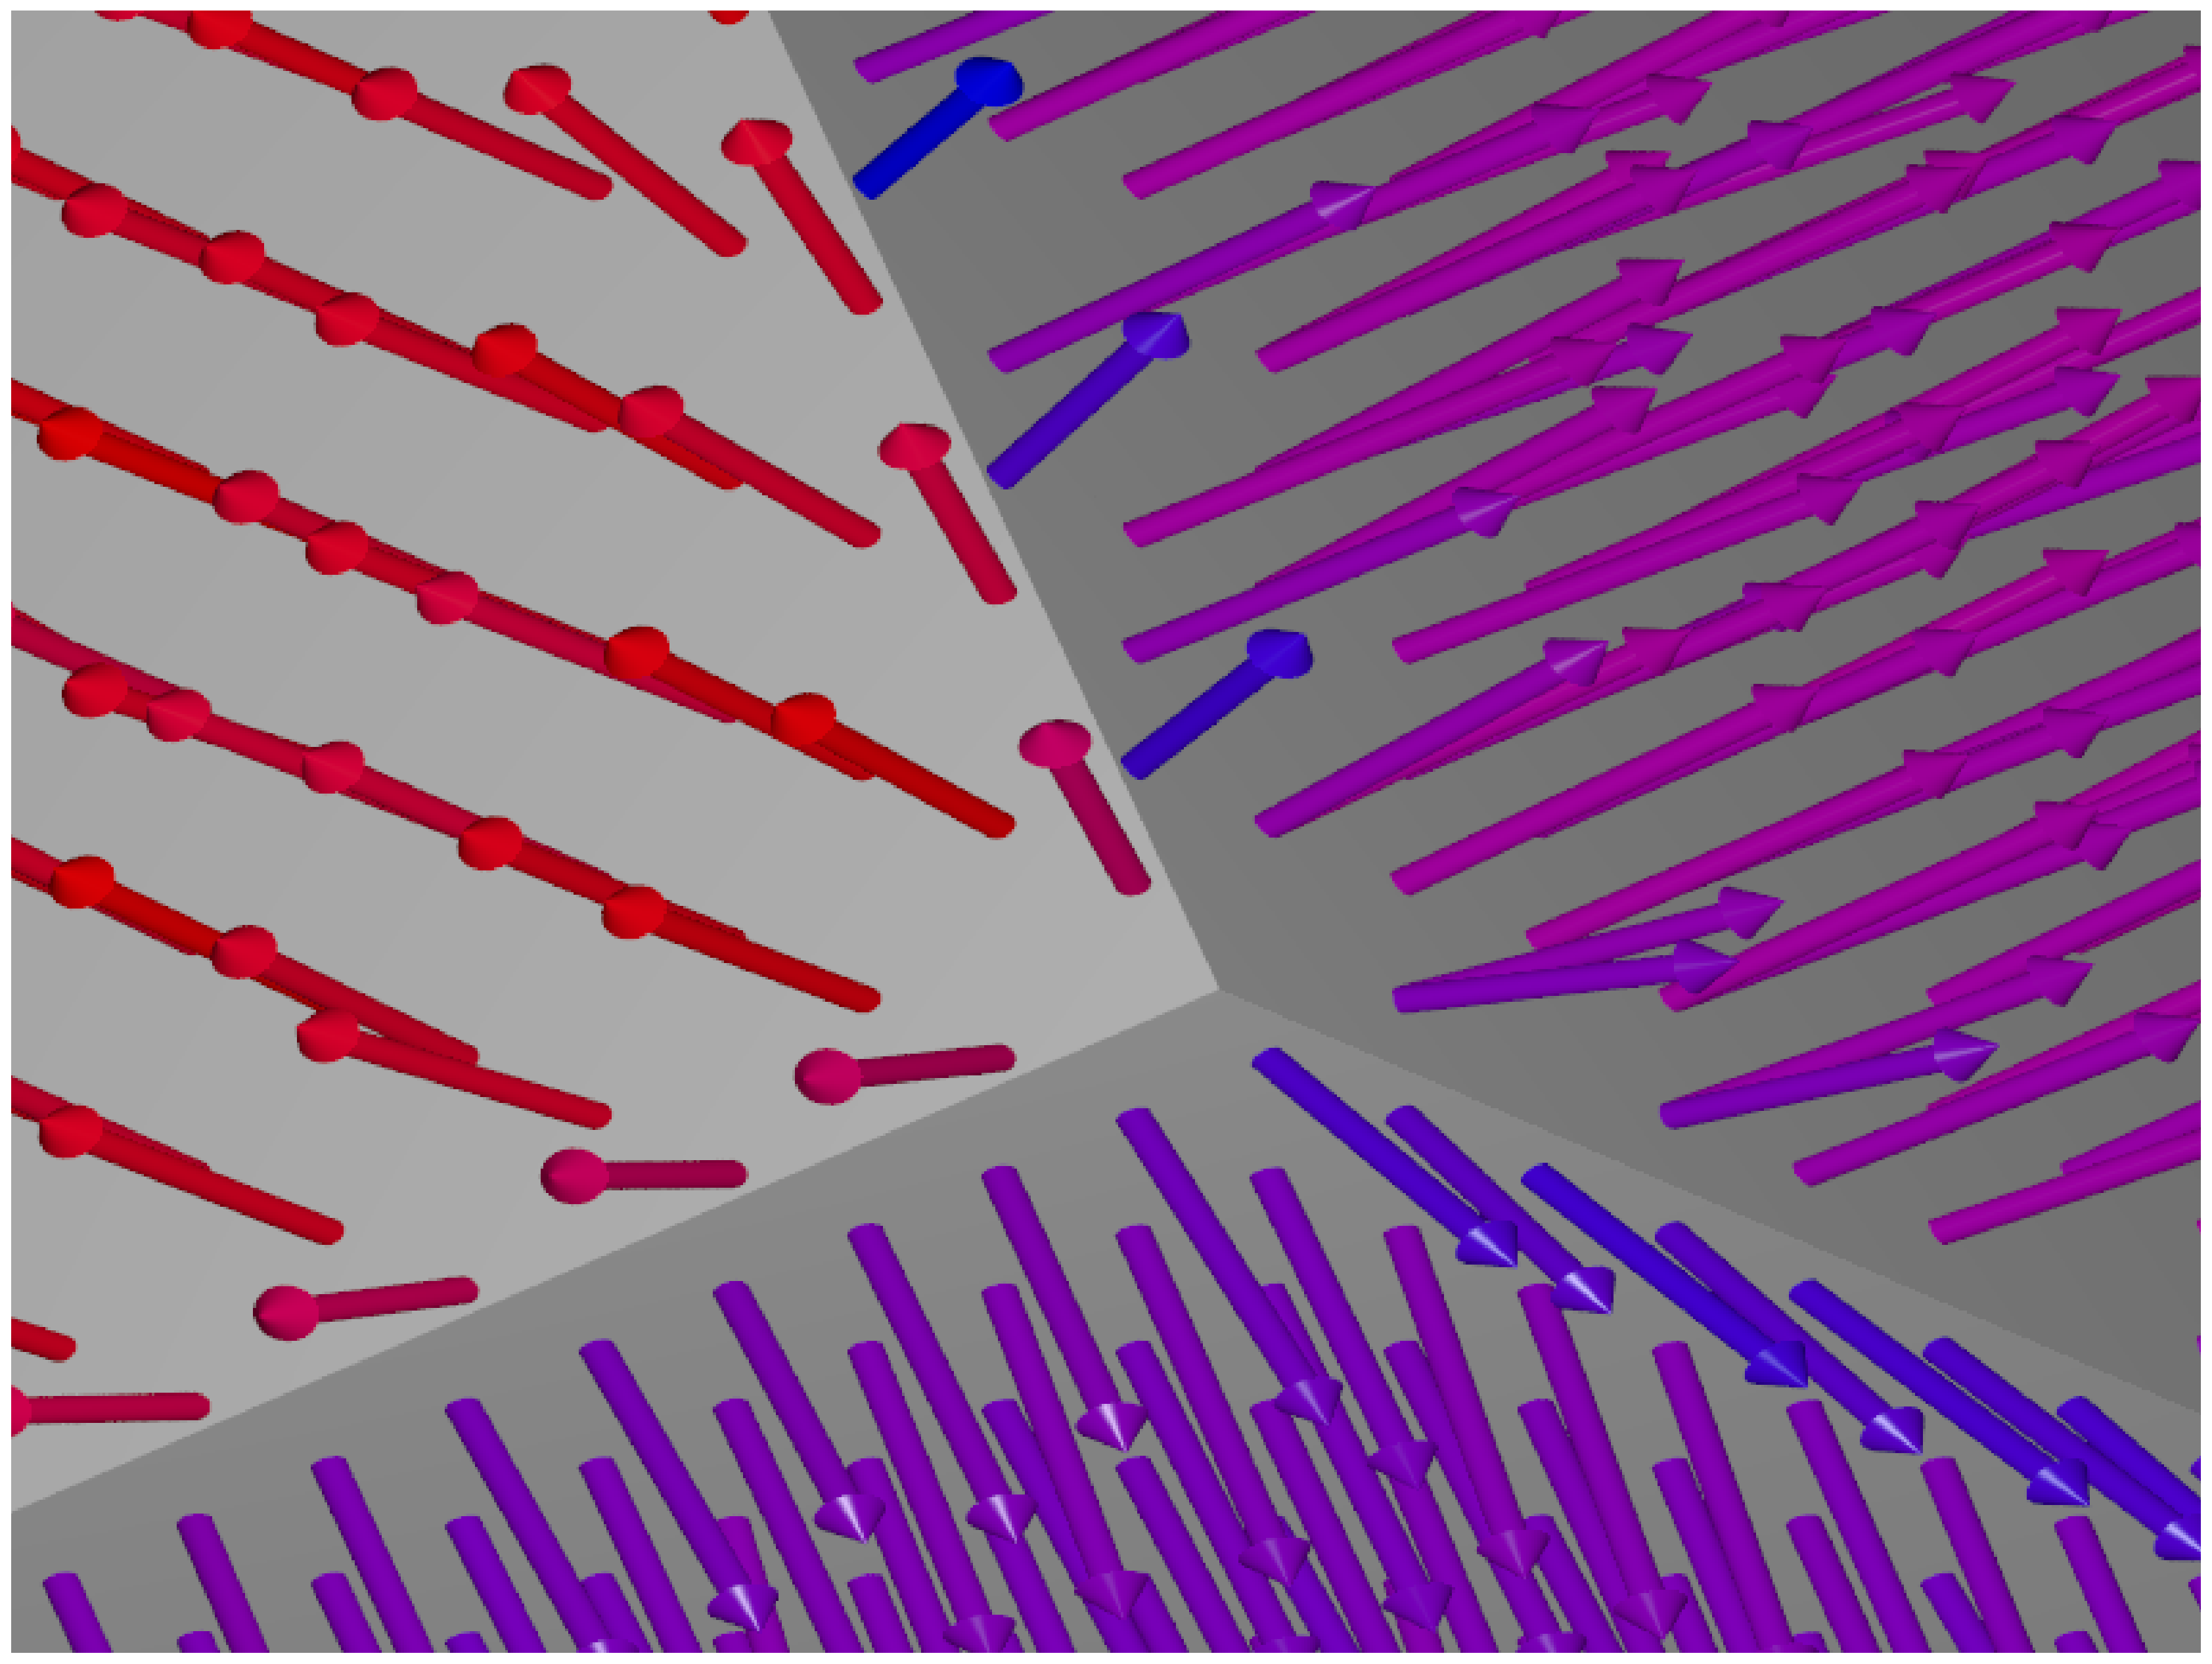
\includegraphics[width=0.25\linewidth]{images/cube.noise.cdiff.eps}\label{fig:cube:noise:cdiff}}
    \subfloat[]{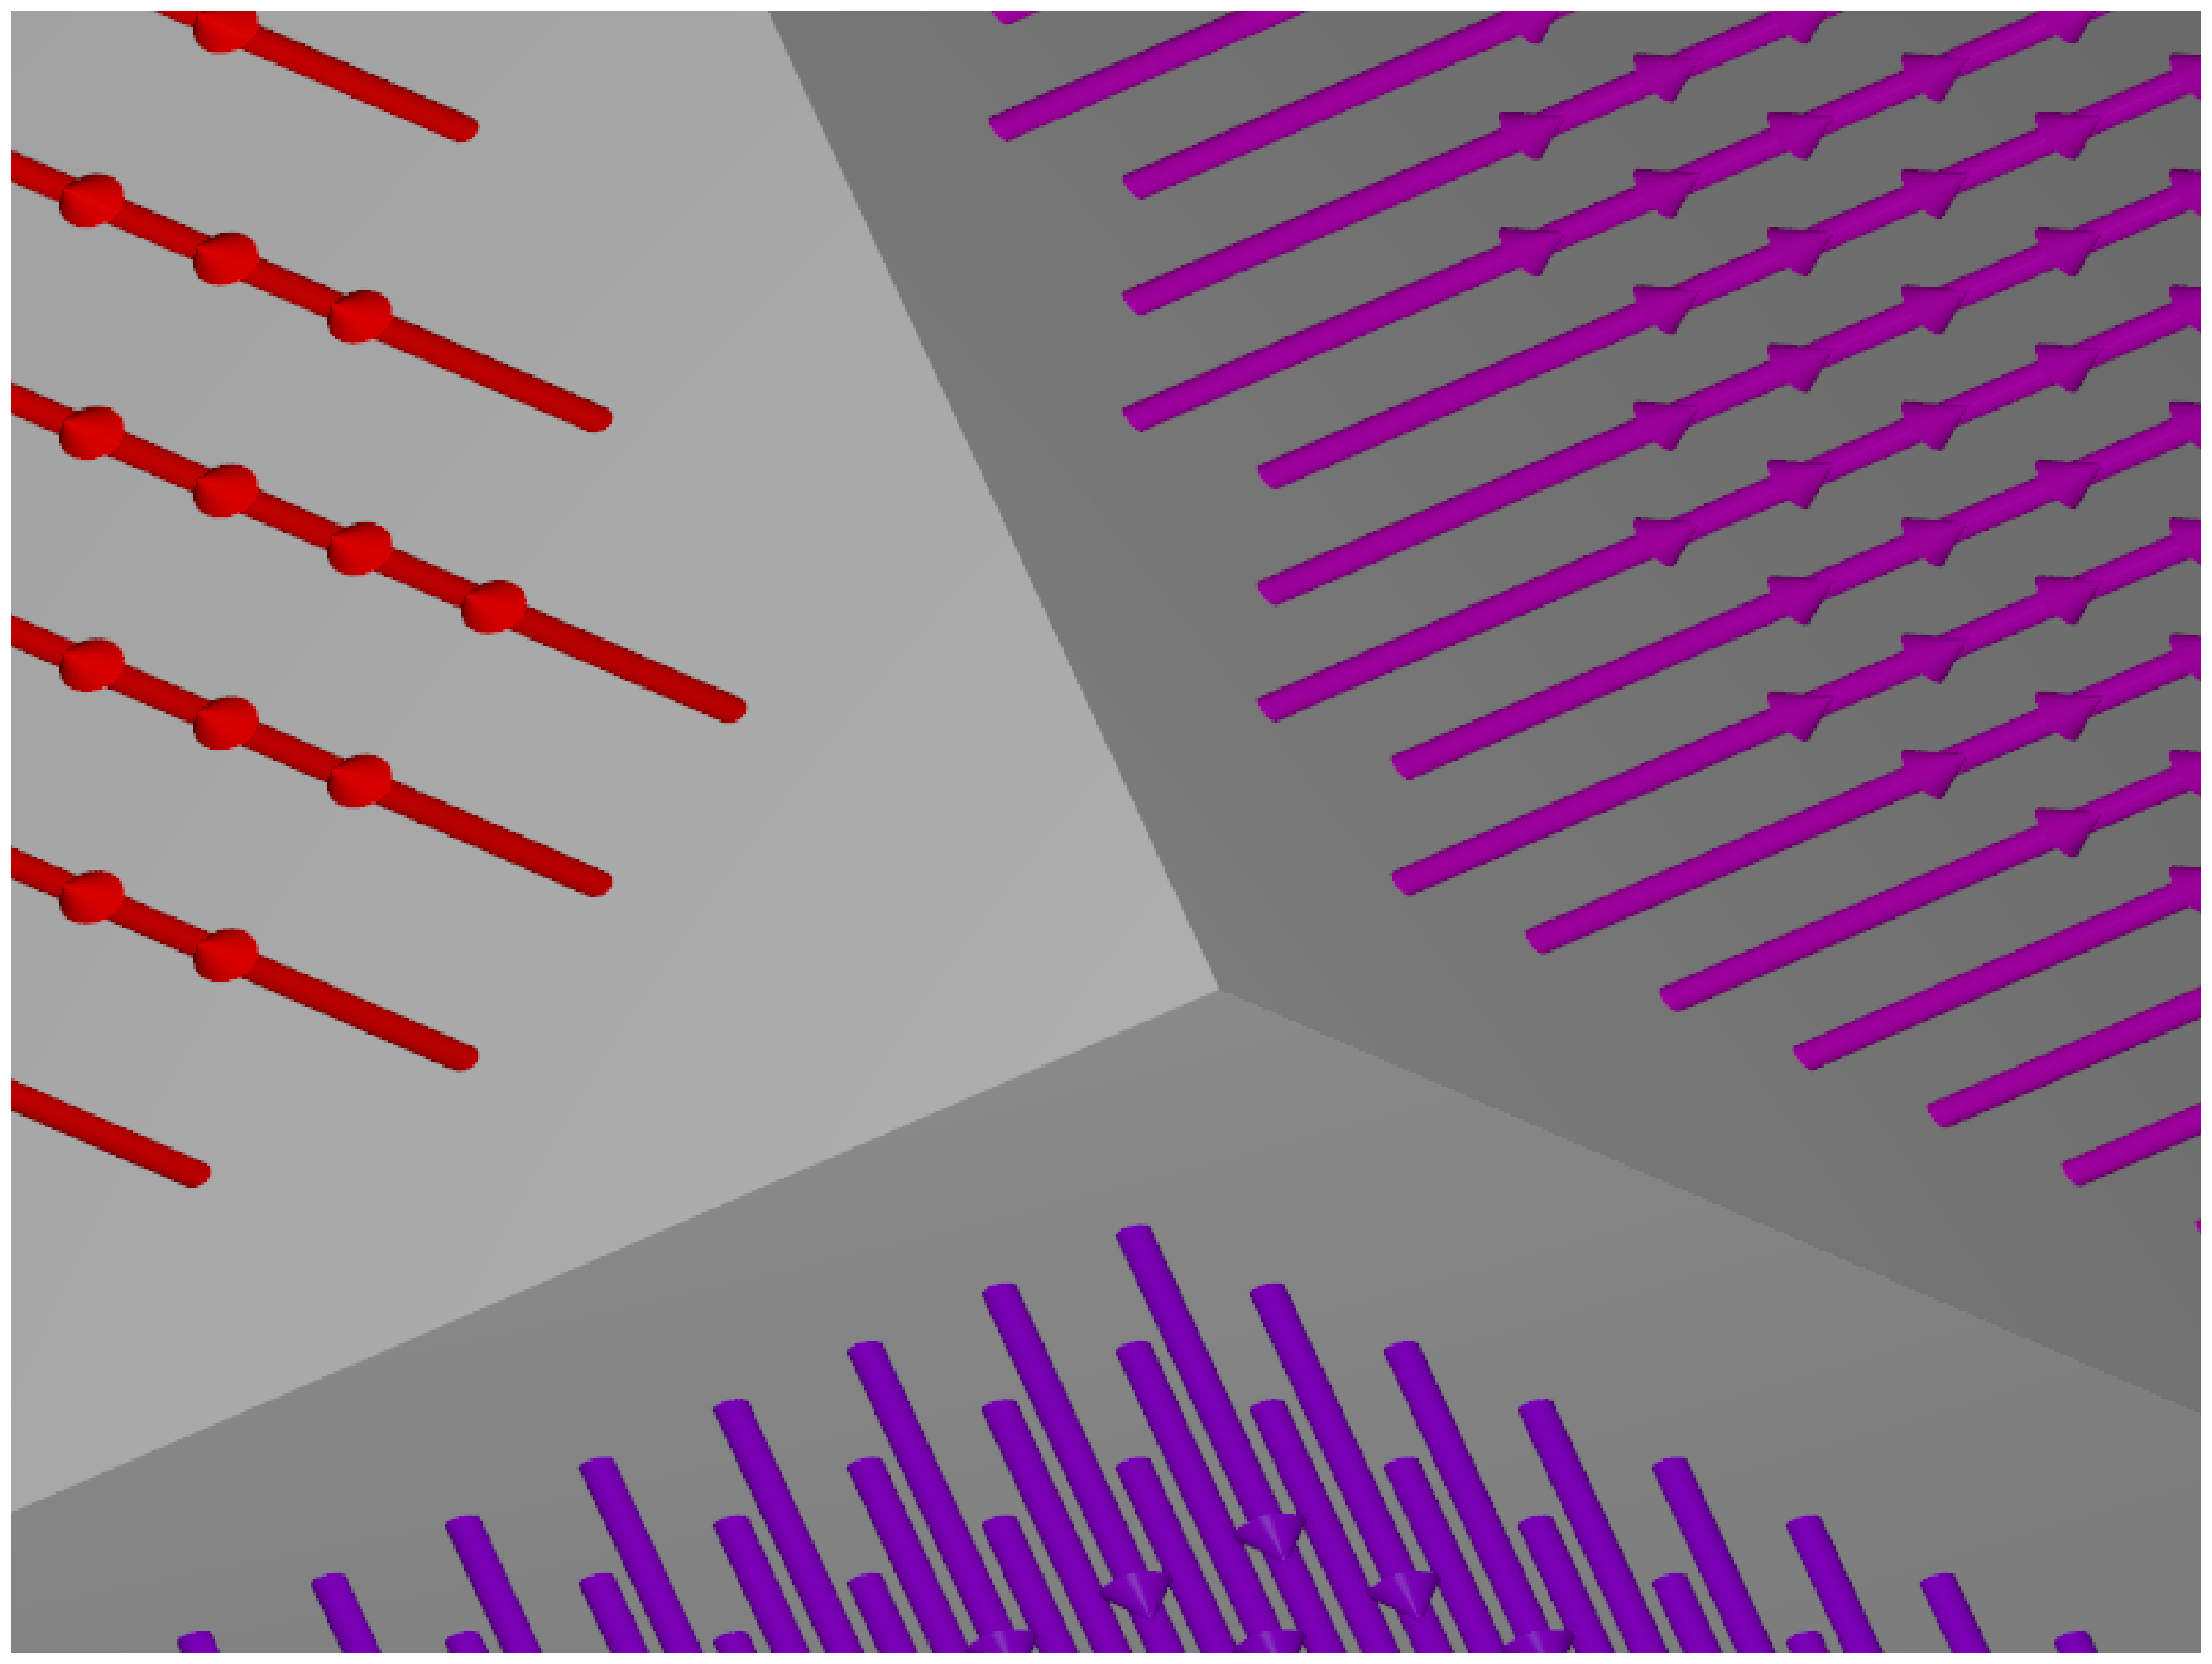
\includegraphics[width=0.25\linewidth]{images/cube.religrad.eps}\label{fig:cube:religrad}}
    \subfloat[]{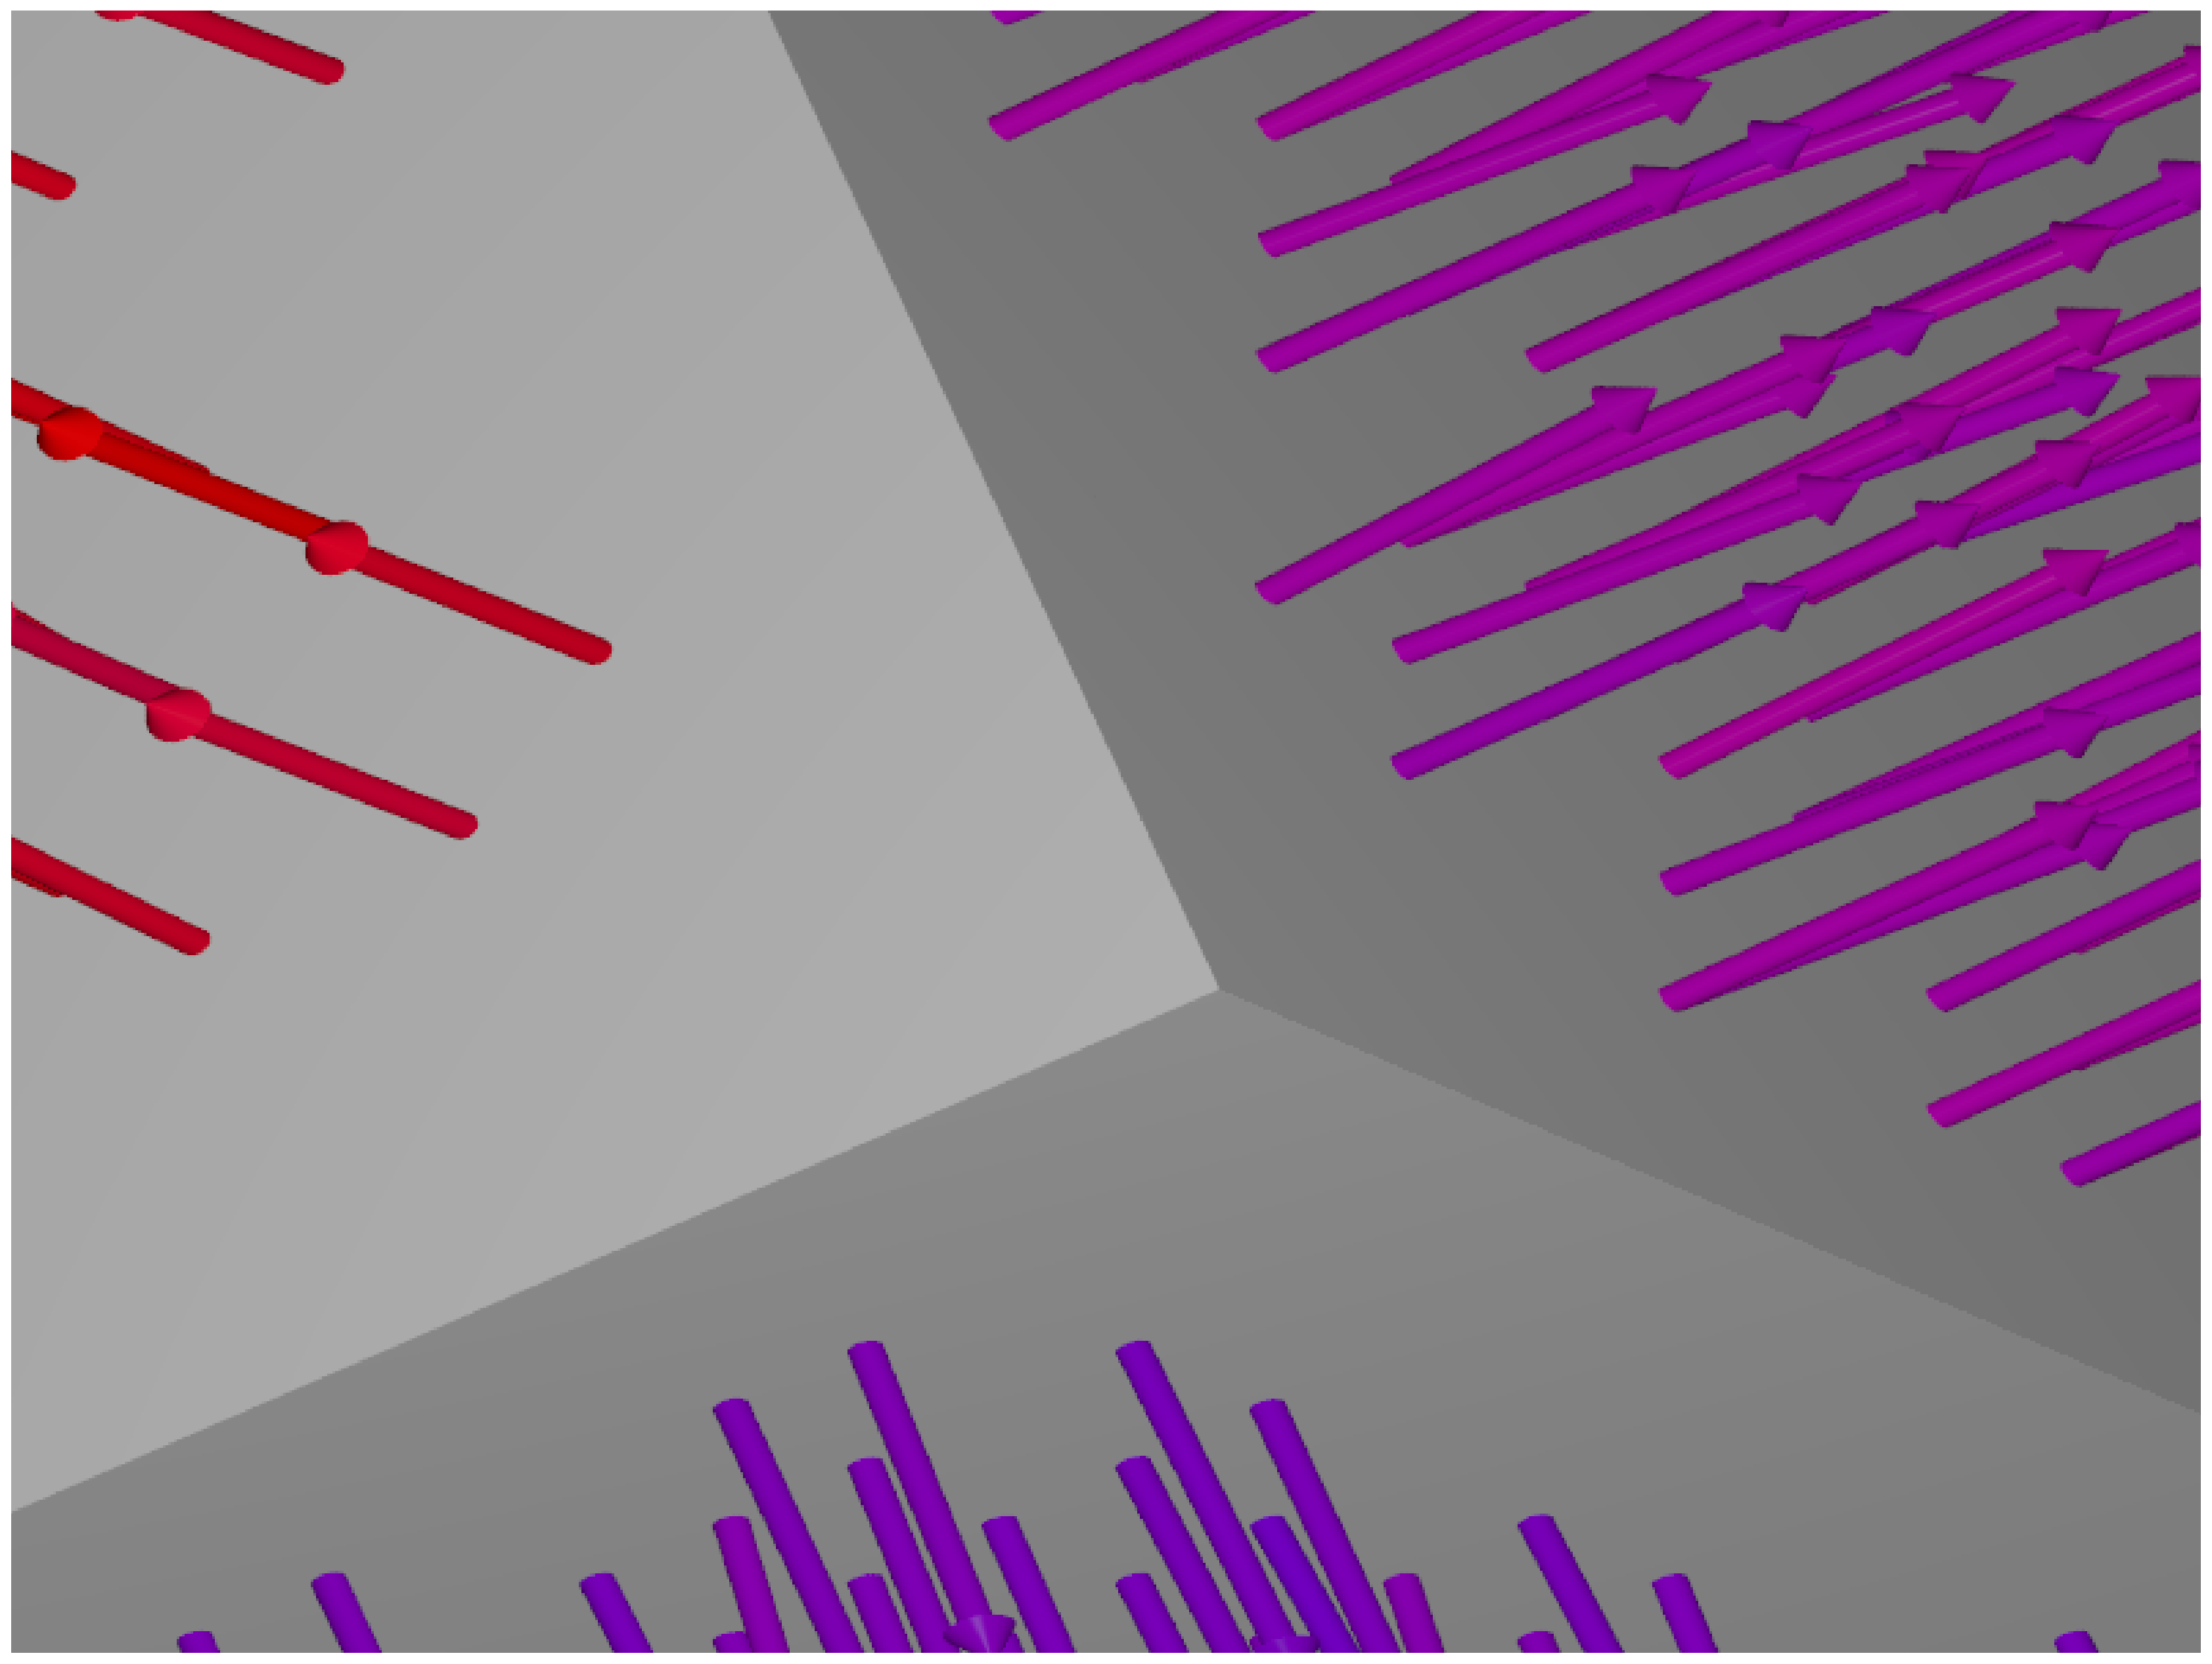
\includegraphics[width=0.25\linewidth]{images/cube.noise.religrad.eps}\label{fig:cube:noise:religrad}}\vspace{-3mm}
    \caption{Effect of uniform noise on \textit{cube} gradients. Uniform 0.1 noise was added to vertex scalars.~\protect\subref{fig:cube:cdiff} central difference gradients on the original \textit{cube}, ~\protect\subref{fig:cube:noise:cdiff}  central difference gradients computed on the noisy cube.
    ~\protect\subref{fig:cube:religrad}  gradients marked correct by \protect\ReliGrad on the original \textit{cube}. ~\protect\subref{fig:cube:noise:religrad} gradients at the vertices marked correct by \protect\ReliGrad on the noisy \textit{cube}. }
    \label{fig:cube:noise}
\end{figure}
Figure~\ref{fig:cube:noise} shows the gradients at corner of the \textit{cube} dataset.
Figure~\subref*{fig:cube:cdiff} shows the central difference gradients. As expected, the gradients across the discontinuity are erroneous.
Figure~\subref*{fig:cube:religrad} shows gradients at grid vertices marked correct by \protect\ReliGrad.
The problems of central difference gradients becomes compounded if the scalar values are noisy. We added 0.1 uniform noise to grid vertex scalars of \emph{cube}. Figure~\subref*{fig:cube:noise:cdiff} shows the central difference  gradients computed from the noisy scalars, Figure~\subref*{fig:cube:noise:religrad} shows the result from \ReliGrad.
\subsection{Quantitative Analysis}
For the synthetic tests cases we know the correct gradients at each grid vertex. Consequently, we can quantitatively compare them with reliable gradients results.
 \begin{table}[h]
     \centering
     \begin{tabular}{|c c c c c c|}
         \hline
         Dataset & CDiff & Algo 1 & Algo 2 & \begin{tabular}[c]{@{}l@{}}Find\\ Reliable\end{tabular} &  \begin{tabular}[c]{@{}l@{}}Reli\\ Grad\end{tabular}\\
         \hline
         Cube  & 48.3 & 0.7& 0.0& 0.0& 0.0\\
         Annulus &  44.03 & 2.79 & 0.02 & 0.02 & 0.02 \\
         Flange & 45.4 & 2.1 & 0.04 & 0.04 & 9.8\\
         TwoCube & 61.86 & 6.1 & 0.0 & 0.0 & 19.8\\
         Cannon & 29.7 & 12.3 & 0.5 & 0.5 & 0.5\\
         Cone & 57.5 & 1.6 & 1.11 & 1.11 & 13.1\\ 
         \hline
       \end{tabular}
       \caption{Maximum Angle difference compared to correct gradients in$^\circ$s. $\alpha$,$\alpha2$ is set to 20$^\circ$. A large number of vertices with high angle difference to the correct gradients, means erroneous gradients are being marked correct. Low angles mean the gradients marked reliable are very close to the correct gradient which is desired outcome.}
       \label{table:gradientDiff}
   \end{table}
Table~\ref{table:gradientDiff} shows the maximum angle difference between the known correct gradients and those computed as reliable gradients at each grid vertex $v$. Intuitively this captures false positives. Large maximum angle would mean poor gradients are being marked as correct.
Algorithm 2 which uses vertices at edge distance 3 for $n_v$ has lower angles than Algorithm 1 for all the test cases thus performing better. Figure~\subref*{fig:annulus:algo1} (Algorithm 1) showed one particular example where gradients near the discontinuity were marked correct compared to (Algorithm 2) Figure~\subref*{fig:annulus:algo2}.  Central difference as expected generates erroneous gradients near the edges. For the synthetic datasets, \FindReliable, performs similarly to Algorithm 2.~\ReliGrad which extends the \FindReliable gradients by using Algorithm ~\ref{alg:extend} generates larger maximum angle than \FindReliable.
\begin{table}[h]
    \centering
    \begin{tabular}{|c c c c |}
        \hline
        Dataset  & Algorithm 1 & Algorithm 2 & \ReliGrad\\
        \hline
        Annulus  & 3 & 4 &  2\\
        Cube & 3 & 4 & 3\\ 
        Flange & 4 & 6 & 4\\
        Cannon & 2& 4& 2\\
        Cone   & 3& 4& 2\\
        TwoCube & 4& 5& 3\\ \hline
    \end{tabular}
    \caption{Maximum of L1 distances to closest grid vertices 
             with exact gradients.}
    \label{table:gradientinfo}
\end{table}

Next we look at the maximum of the L1 distances from each vertex $v$ to the closest grid vertex with a reliable gradient.
Table~\ref{table:gradientinfo} shows the results. This test intuitively captures false negatives. Large distances mean more vertices with reliable gradients are being marked unreliable. 
It is desirable for algorithms which use the reliable gradients results, that the L1 distance of  an unreliable vertex $v$ to its closest reliable vertex $v_2$ be as small as possible. For \textit{Annulus} there is a grid vertex at maximum L1 edge distance of 4 from each $v$ when using Algorithm~\ref{alg:phi2}. For \textit{Cube} there is a vertex with correct gradient within L1 edge distance 4 from each $v$ when using Algorithm~\ref{alg:phi2}. When we extend the reliable gradients and use \ReliGrad,  the maximum L1 distance decreases to 2 and 3 respectively. 
Experimentally we found 
that the distances for \textit{Cube} is maximum near the corners.
(See  Figure~\subref*{fig:cube:religrad}.)

\textbf{Noise}:
To test the effect of noise on \ReliGrad, uniform noise was added to the datasets. Table~\ref{table:noise} shows the results. With 0.1 uniform noise \ReliGrad performs well. 
The maximum $L_1$ distance to reliable gradients in the \textit{Cube} dataset 
is 5.
This distance was achieved at a vertex near the isosurface corner
(Figure~\subref*{fig:cube:noise:religrad}.) 
With a high uniform noise of 0.2 and $\alpha_{2}$ set to 30 degrees, 
\ReliGrad performs reasonably well. 
\tiny
\begin{table}[htb]
    \begin{center}

    \begin{tabular}{|l|l|l|l|l|}
        \hline
        dataset & noise & \begin{tabular}[c]{@{}l@{}}$\alpha_{2}$\\ in $^{\circ}$\end{tabular} & \begin{tabular}[c]{@{}l@{}}Max\\ AngleDiff in $^{\circ}$\end{tabular} & \begin{tabular}[c]{@{}l@{}}Dist\\ 2Grad\end{tabular} \\ \hline
        cube    & 0.1   & 20                                                                   & 7.5                                                                  & 5         \\ \hline
        annulus & 0.1   & 20                                                                   & 8.1                                                                  & 3         \\ \hline
        cone    & 0.1   & 20                                                                   & 12.7                                                                 & 3         \\ \hline
        cube    & 0.2   & 30                                                                   & 12.8                                                                 & 7         \\ \hline
        annulus & 0.2   & 30                                                                   & 14.1                                                                 & 5         \\ \hline
        cone    & 0.2   & 30                                                                   & 19                                                                   & 6         \\ \hline
    \end{tabular}
    	\caption{Results after adding 0.1 and 0.2 uniform noise to the datasets using \protect\ReliGrad. To handle 0.2 noise we set $\alpha_{2}$ to be 30$^{\circ}$s. MaxAngleDiff, measures the maximum angle difference between known correct gradients and those marked correct by \protect\ReliGrad. Dist2Grad measures the maximum of the l1 distance of the unreliable vertices to vertices marked correct by \protect\ReliGrad.}
        \label{table:noise}
            \end{center}
\end{table}
\normalsize
\subsection{Industrial CT data} 
\tiny
\begin{table}
	\centering
	\begin{tabular}{|c c c |} 
		\hline
		Name & Axis Size & Spacing  \\ [0.5ex] 
		\hline
        CMM & 500 500 196 & 0.2 0.2 0.31\\
		Engine cylinder & 201 130 63 & 0.27 0.27 0.68 \\
        Intake &  150 220 201 & 0.27 0.27 0.68 \\
        Socket & 411 431 61 & 1 1 1 \\
		\hline
	\end{tabular}
	\caption{CT dataset information}
	\label{table:ictDataInfo}
\end{table}
\normalsize

\begin{figure}[htb]
    \centering
    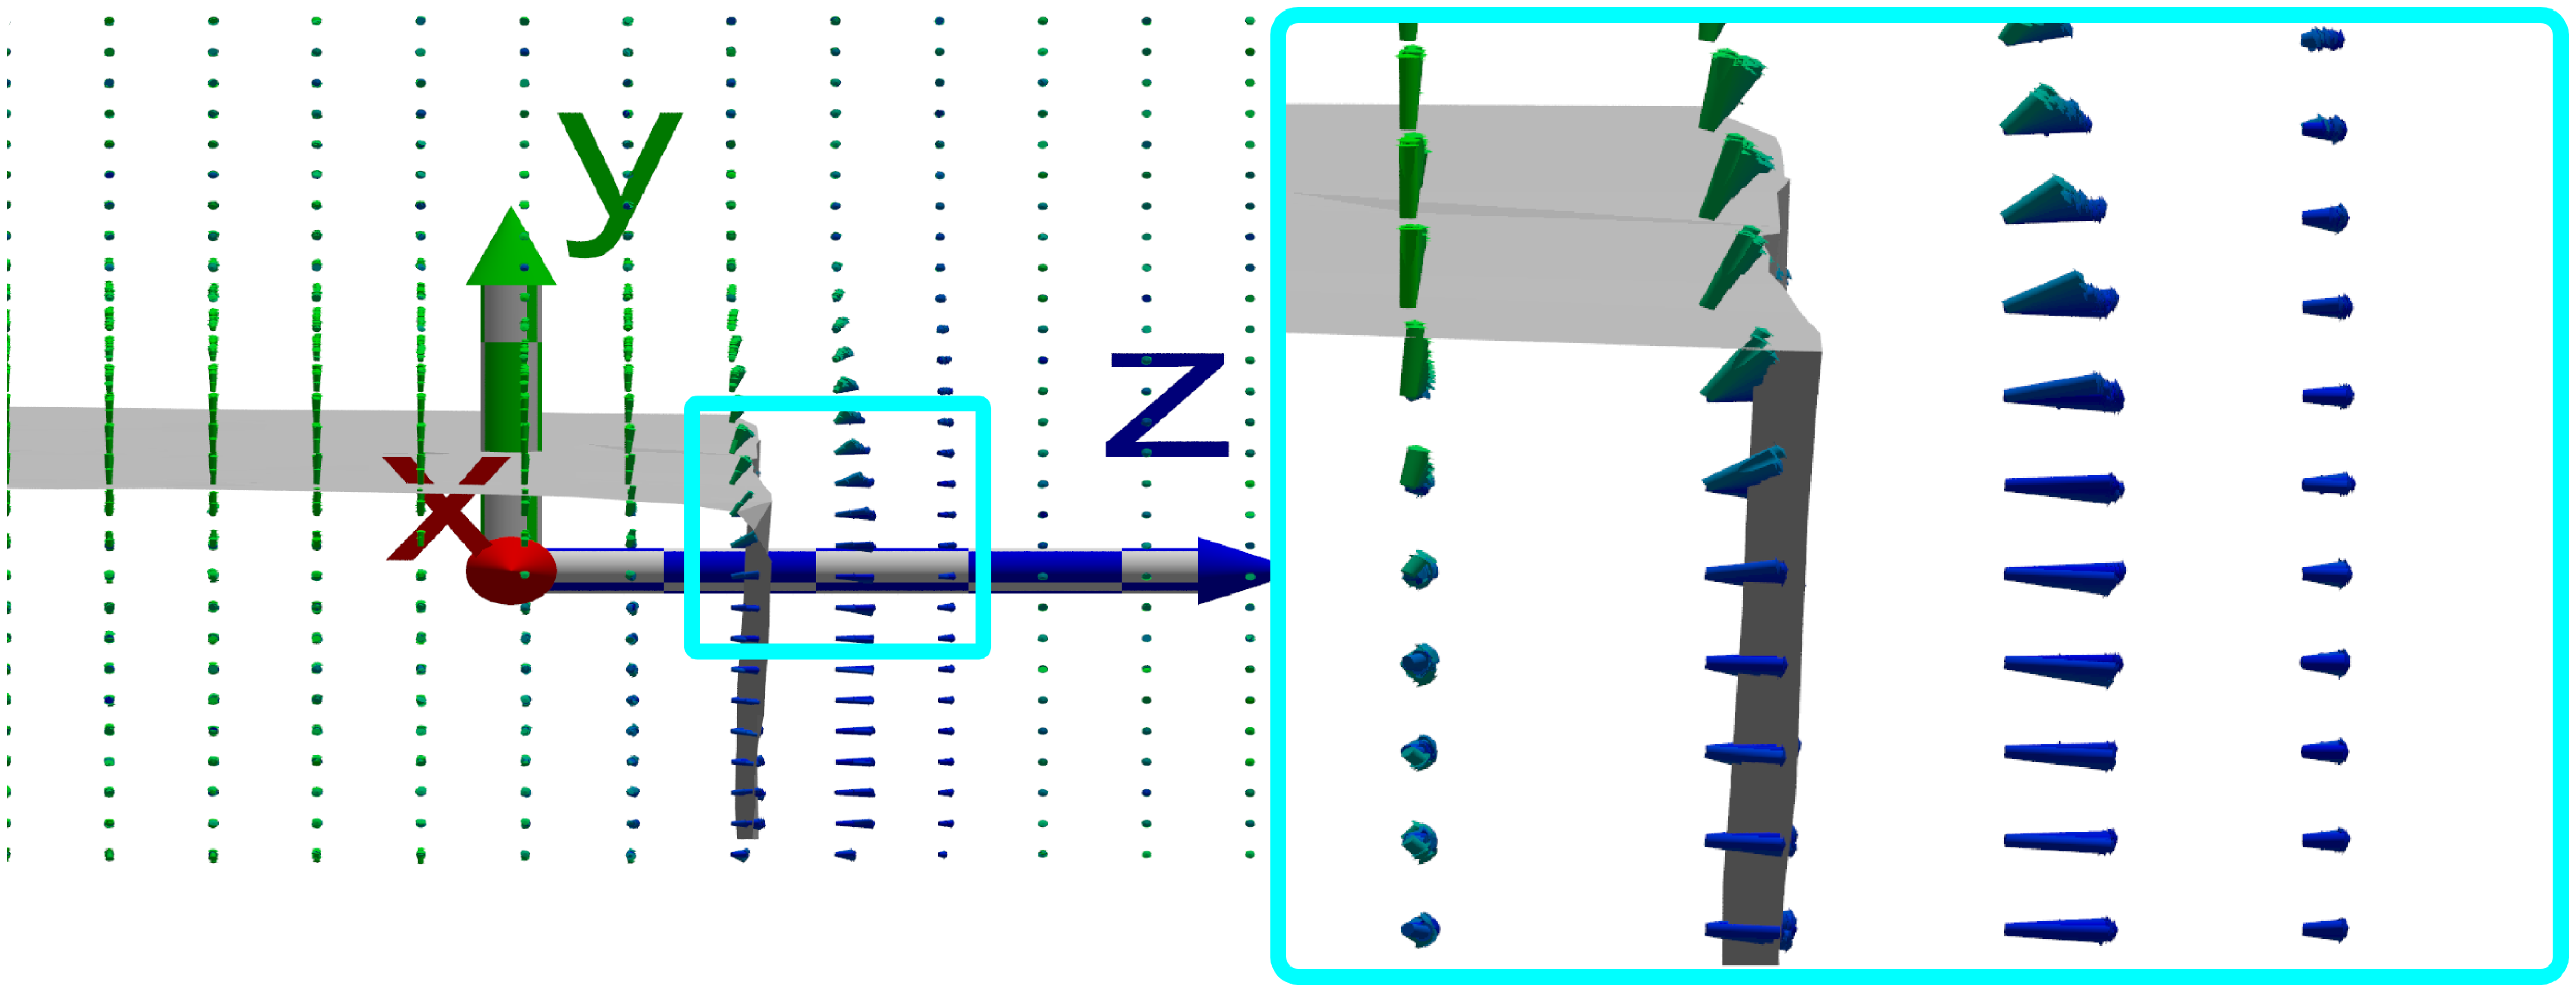
\includegraphics[width=\linewidth]{images/cdiff.all.new.eps}
    \caption{All the central difference gradients on  grid vertices of a small portion of the \textit{engine cylinder} dataset
	(Figure~\ref{fig:grad-1} shows the same regions, 
	but only the gradients at vertices intersected by isosurface).
	The gradient magnitudes are proportional to length of the vectors.
	On the right we see a magnified section of the cyan rectangle.
    The grid magnitudes drop off quickly, and the gradient directions become meaningless especially along the Z-axis. 
    }
    \label{fig:setA.crop1.cdiff}
\end{figure}

\begin{figure}
    \centering
    \subfloat[]{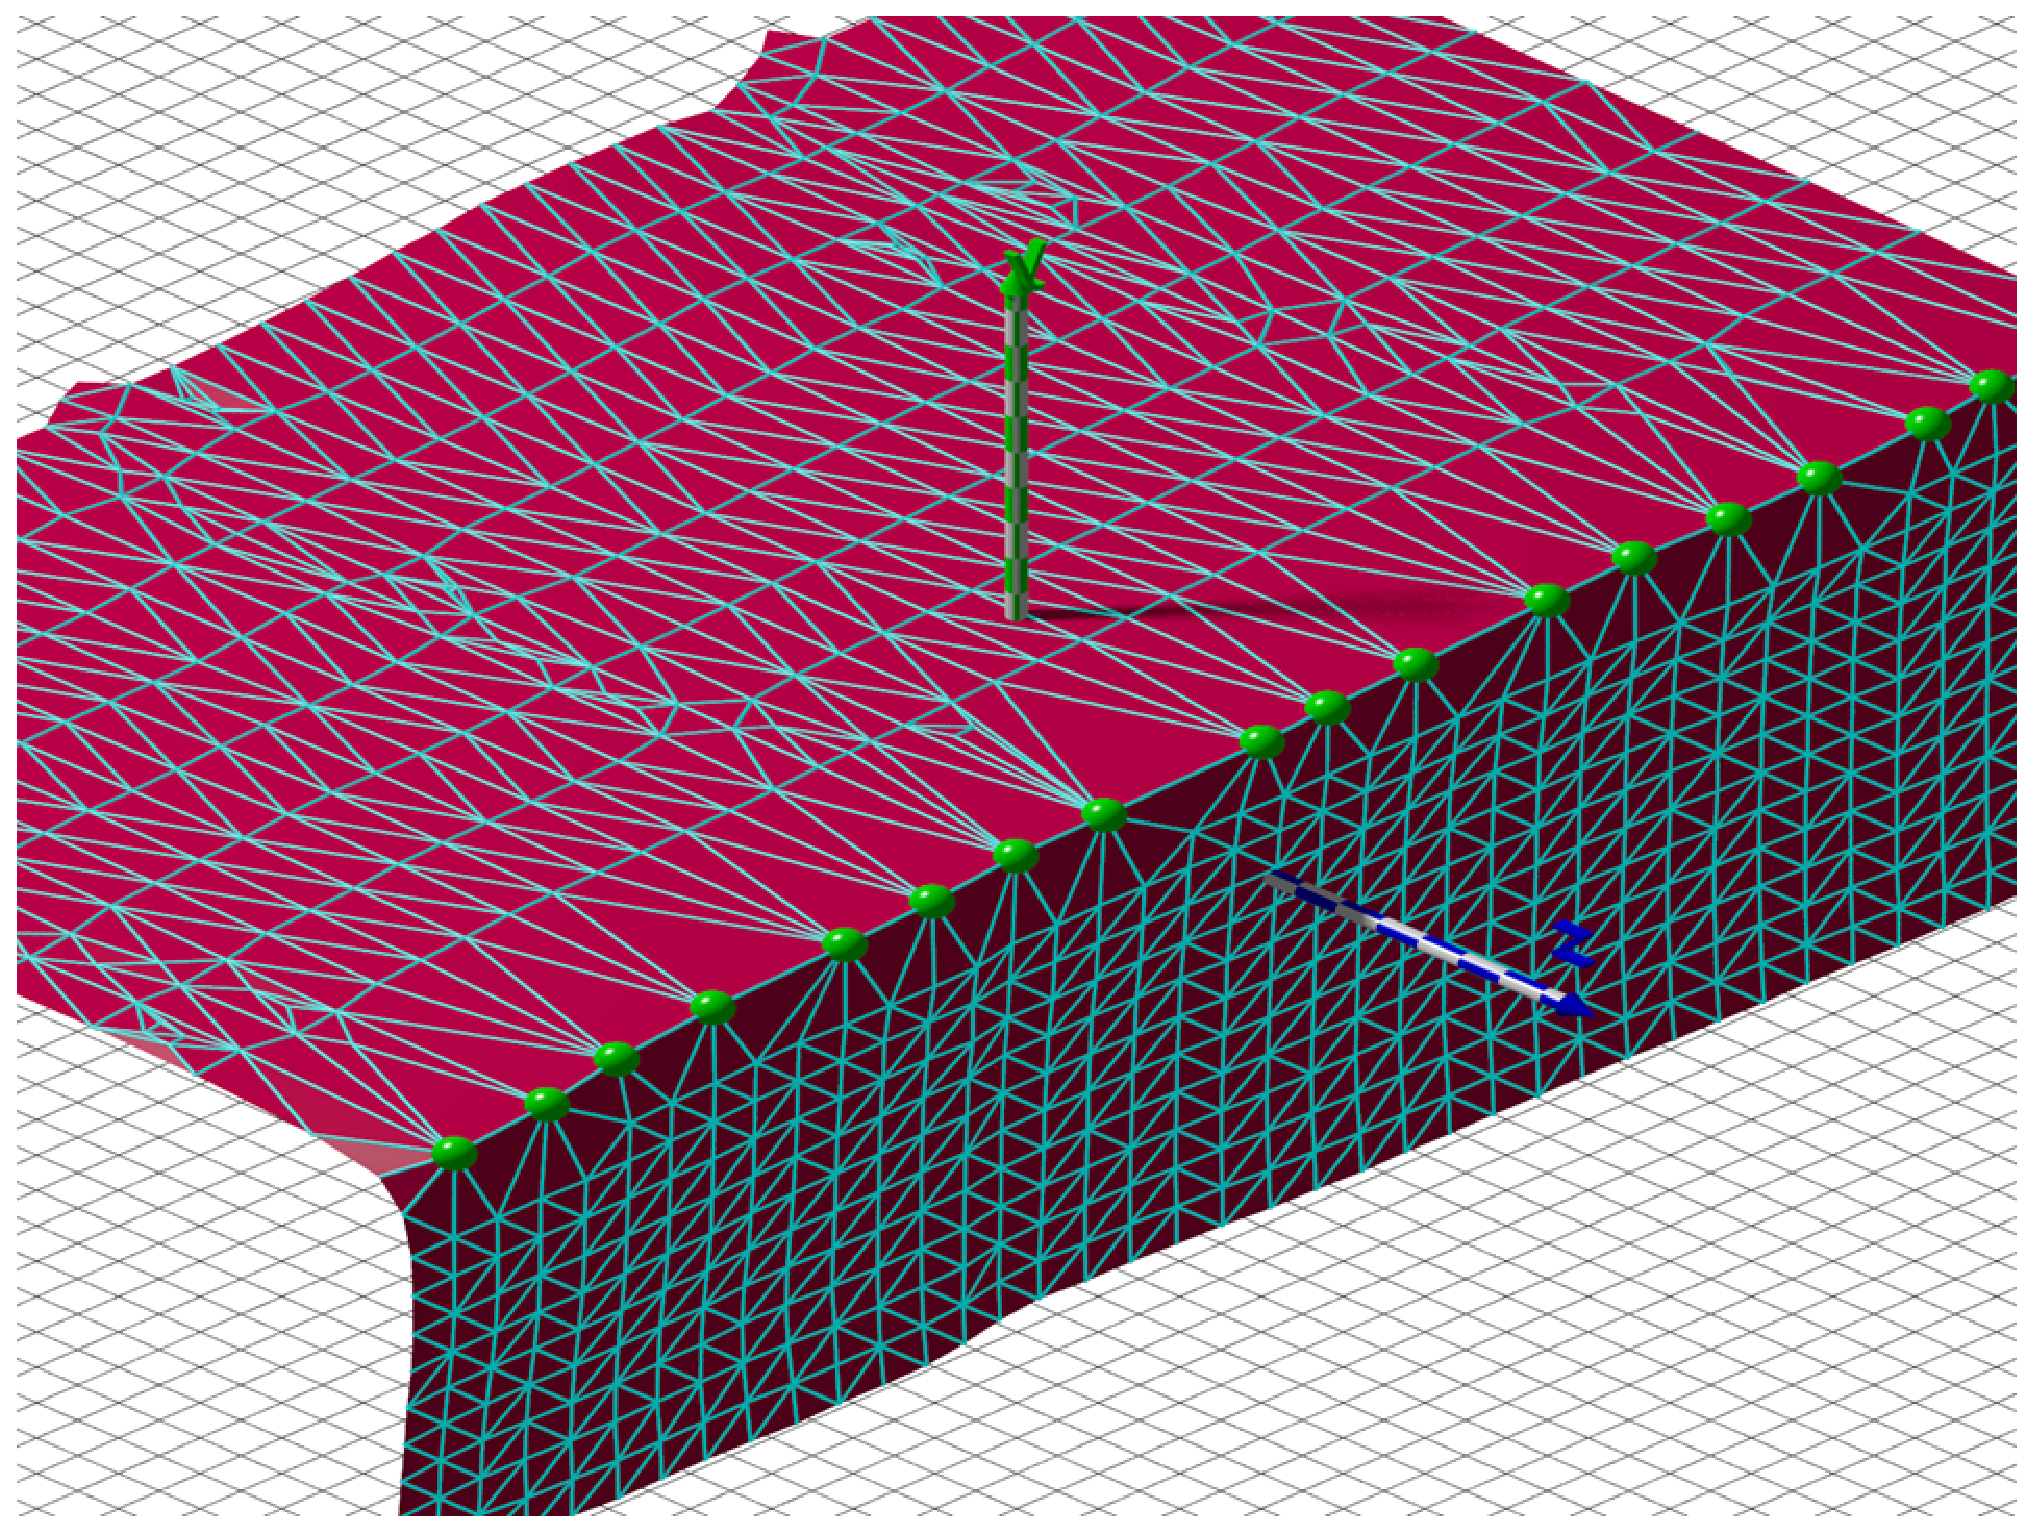
\includegraphics[width=0.33\linewidth]{images/setA.crop2.mesh.eps}\label{fig:setA.crop1.mesh.1}}
    \subfloat[]{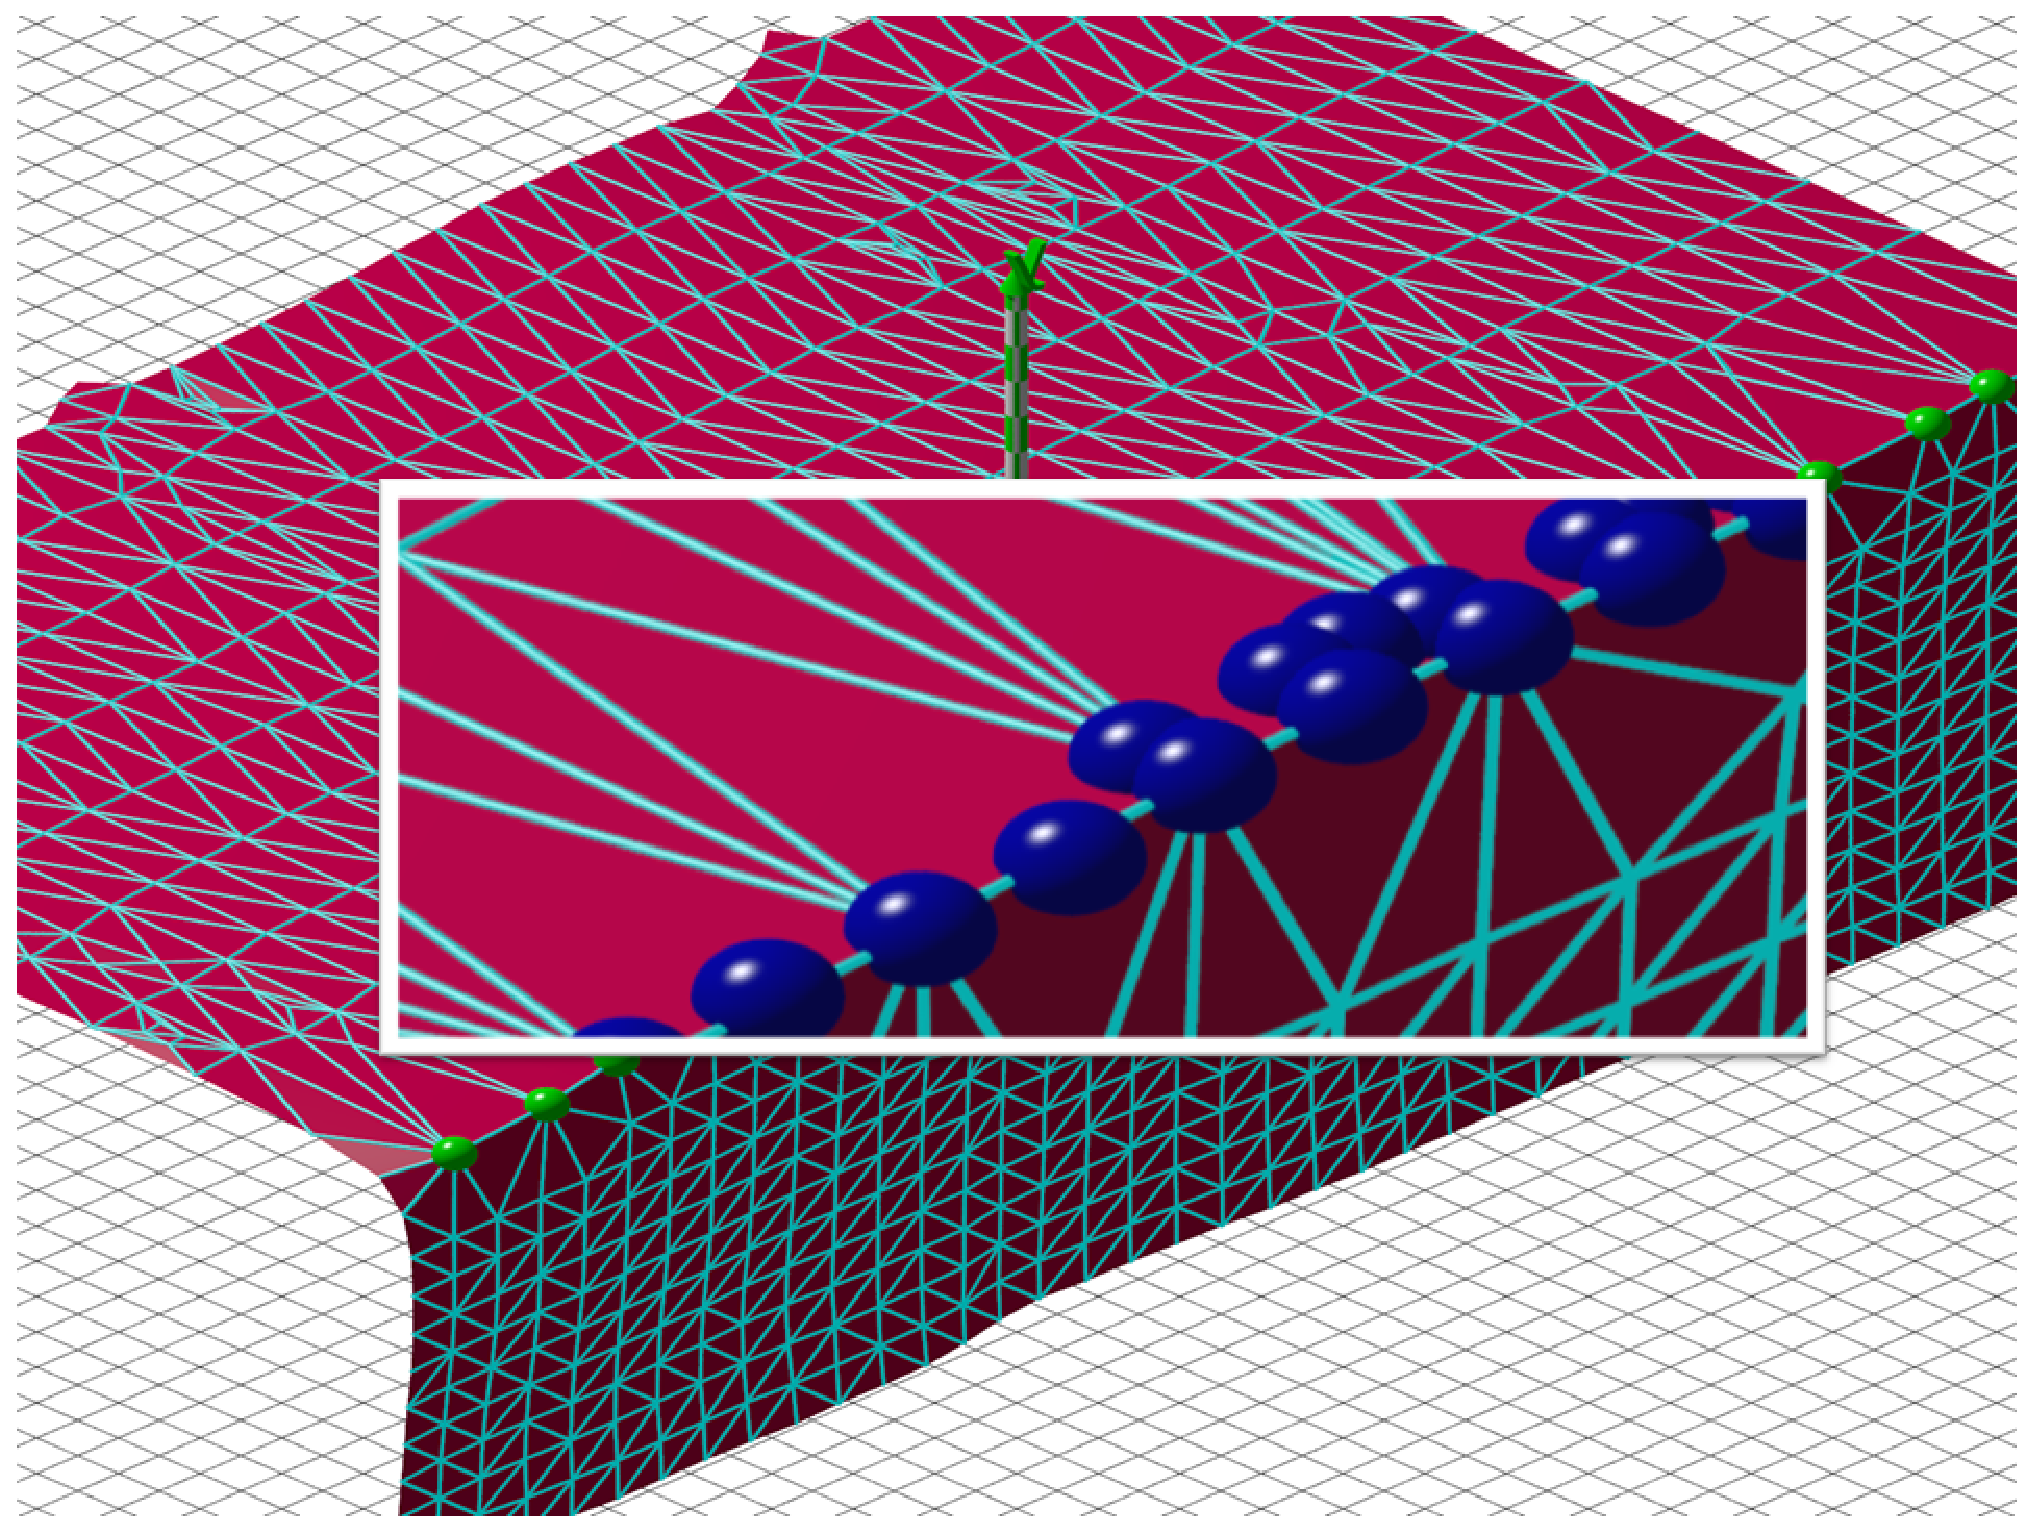
\includegraphics[width=0.33\linewidth]{images/mesh.edges.all.eps}\label{fig:setA.crop1.mesh.2}}
    \subfloat[]{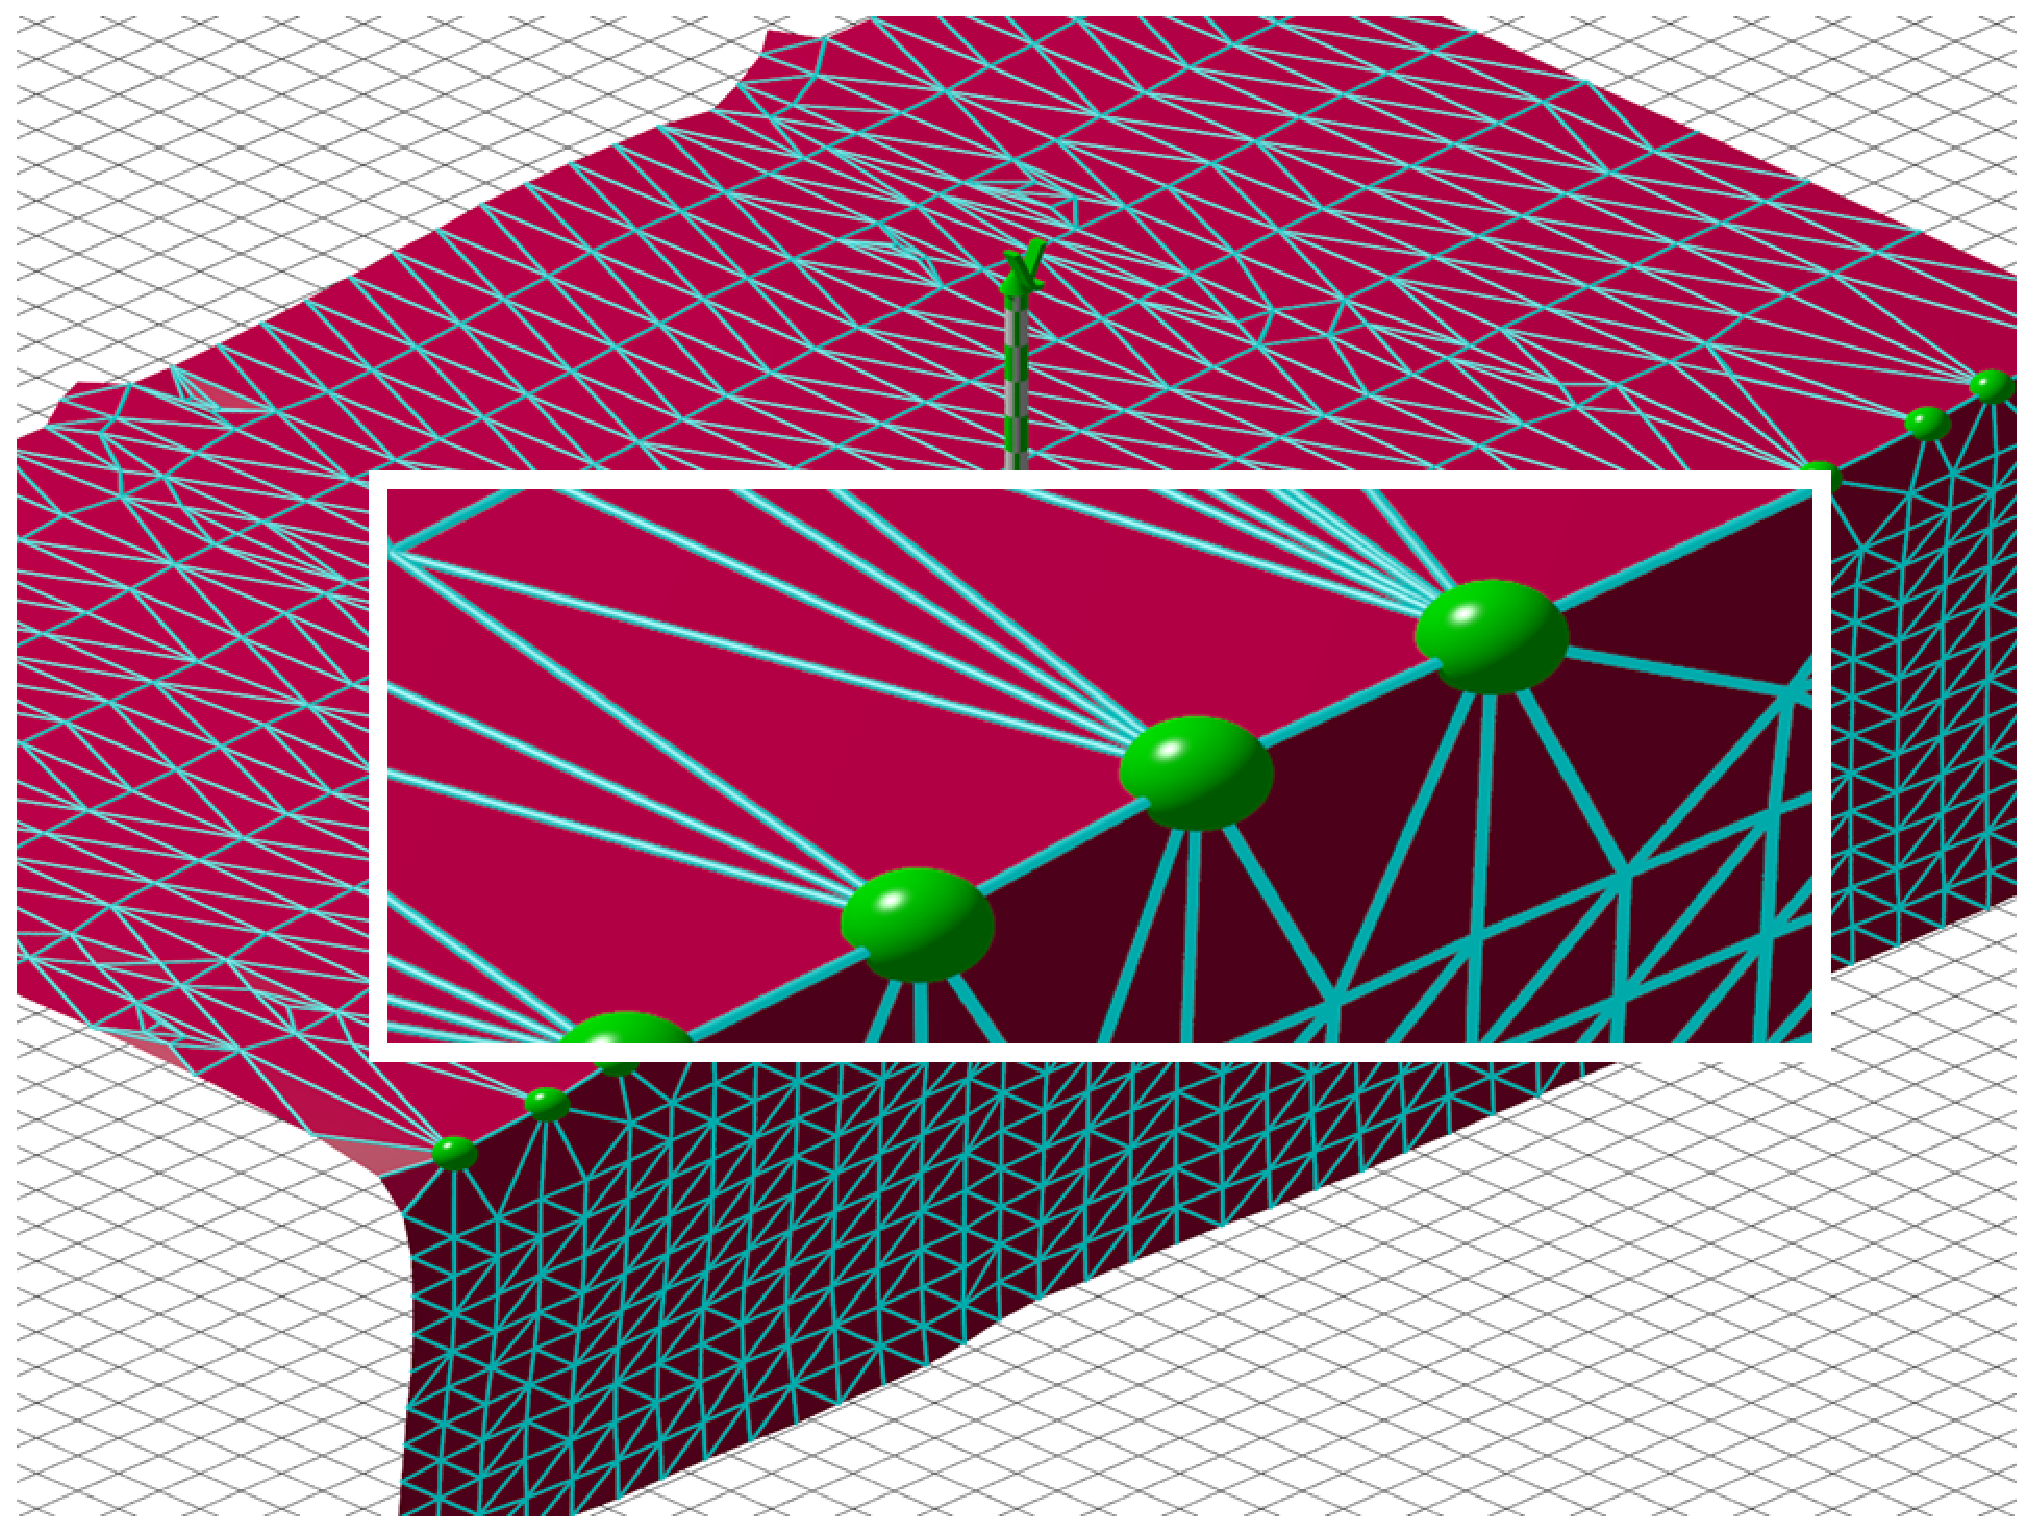
\includegraphics[width=0.33\linewidth]{images/mesh.edges.eps}\label{fig:setA.crop1.mesh.3}}
   \caption{(a) Sharp mesh of a part of (Figure~\ref{fig:setA.crop1}).
       (b) All the sharp edge vertices generated.
       (c) Sparse sharp vertex set}
   \label{fig:setA.crop1.mesh}
\end{figure}
\begin{figure}
    \centering
     \subfloat[Algorithm 1]
     {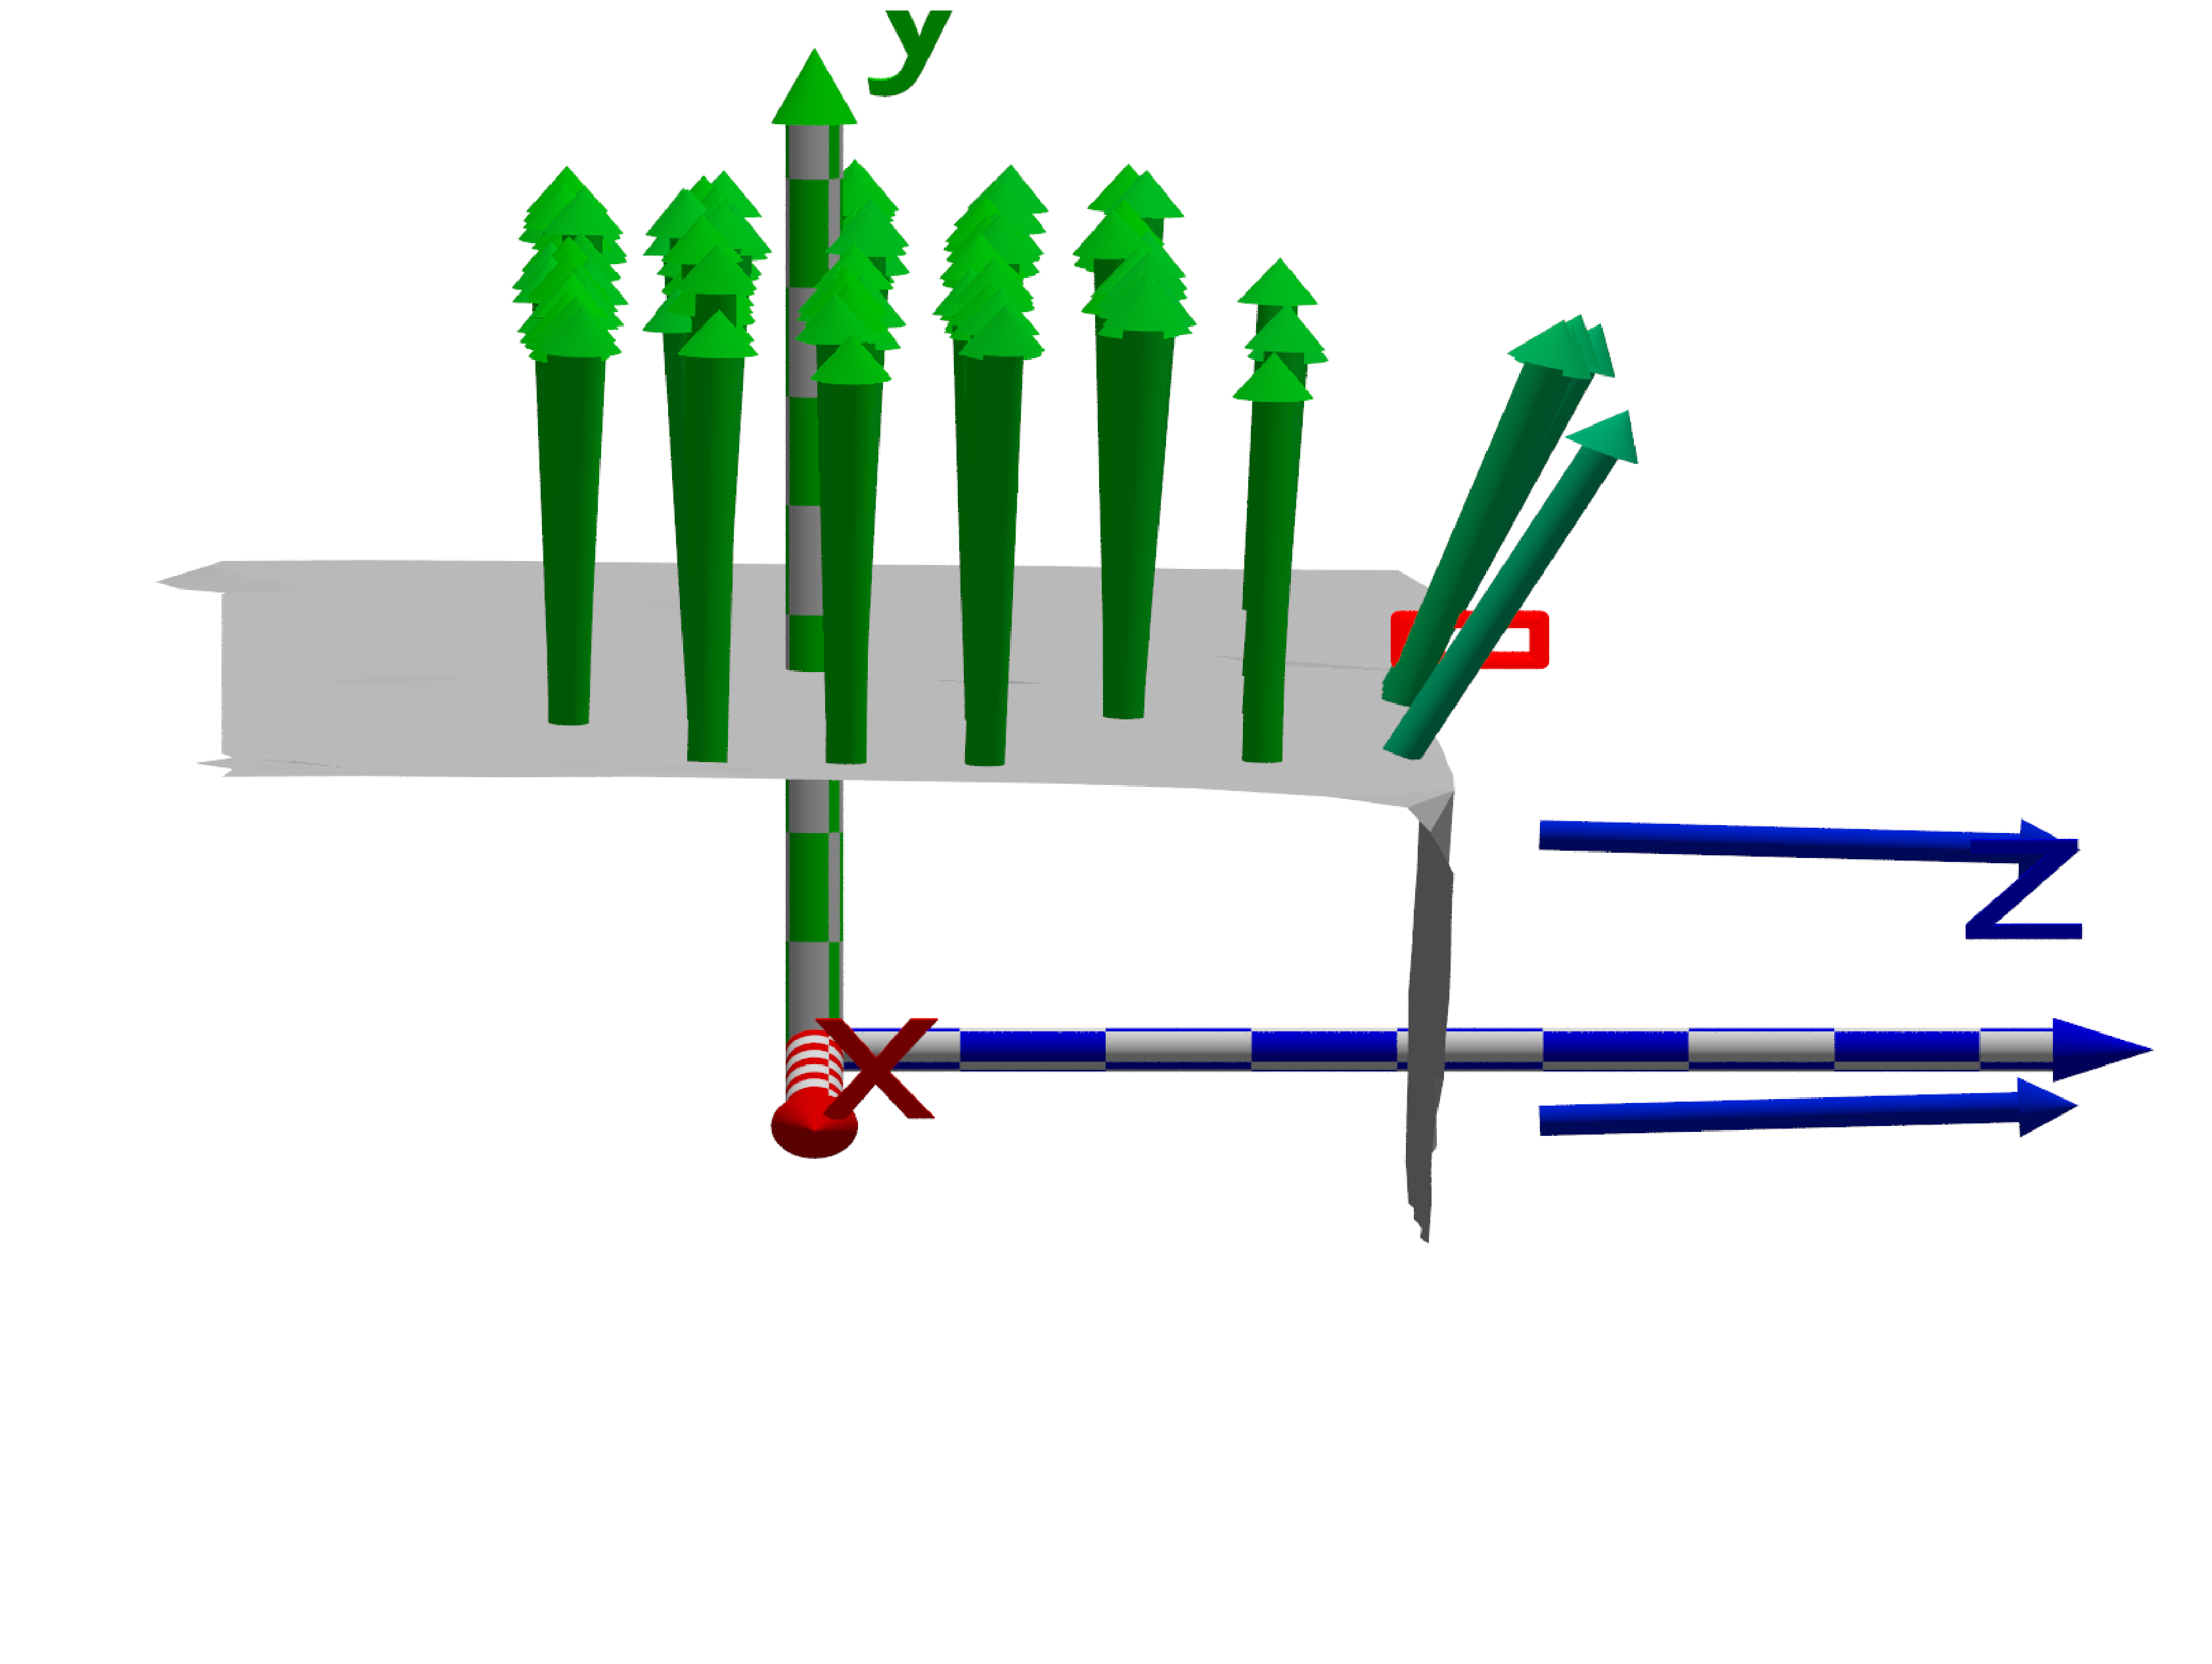
\includegraphics[width=0.25\linewidth ]{images/setA.crop2.algo1.new.eps}\label{fig:setA.crop1.algo1}}
     \subfloat[Algorithm 2]{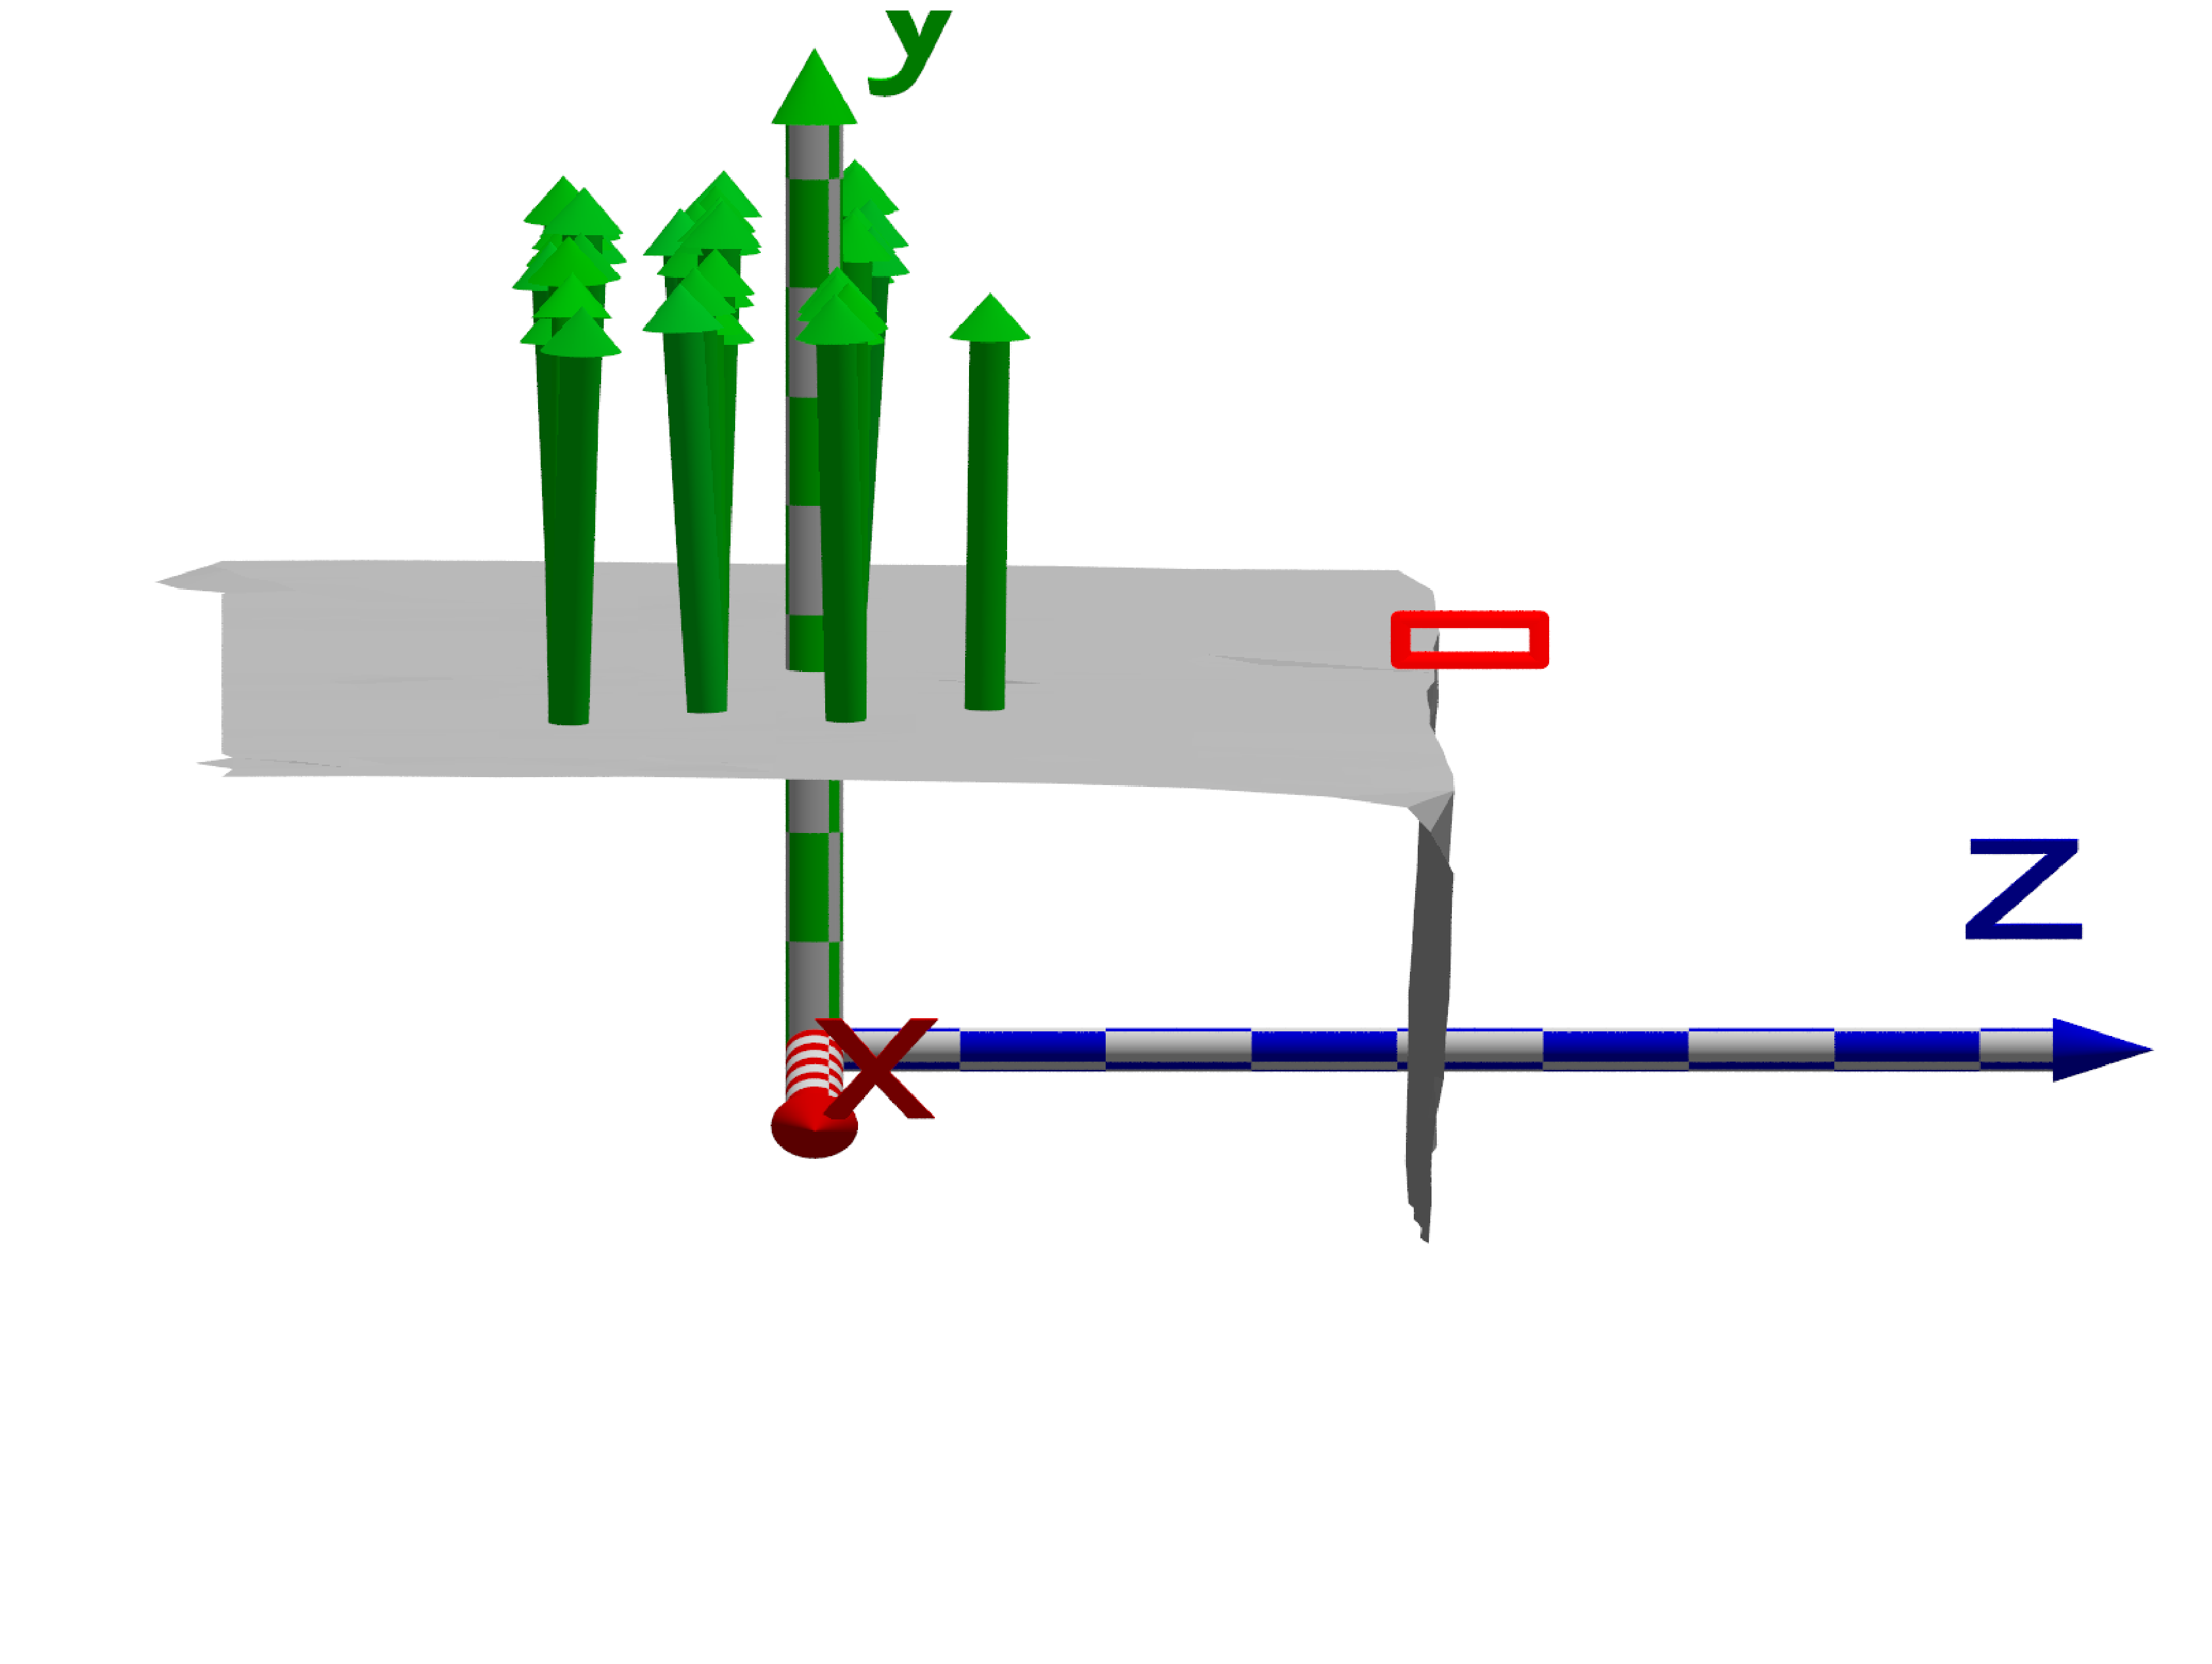
\includegraphics[width=0.25\linewidth]{images/setA.crop2.algo2.new.eps}\label{fig:setA.crop1.algo2}}
     \subfloat[FindReliable]{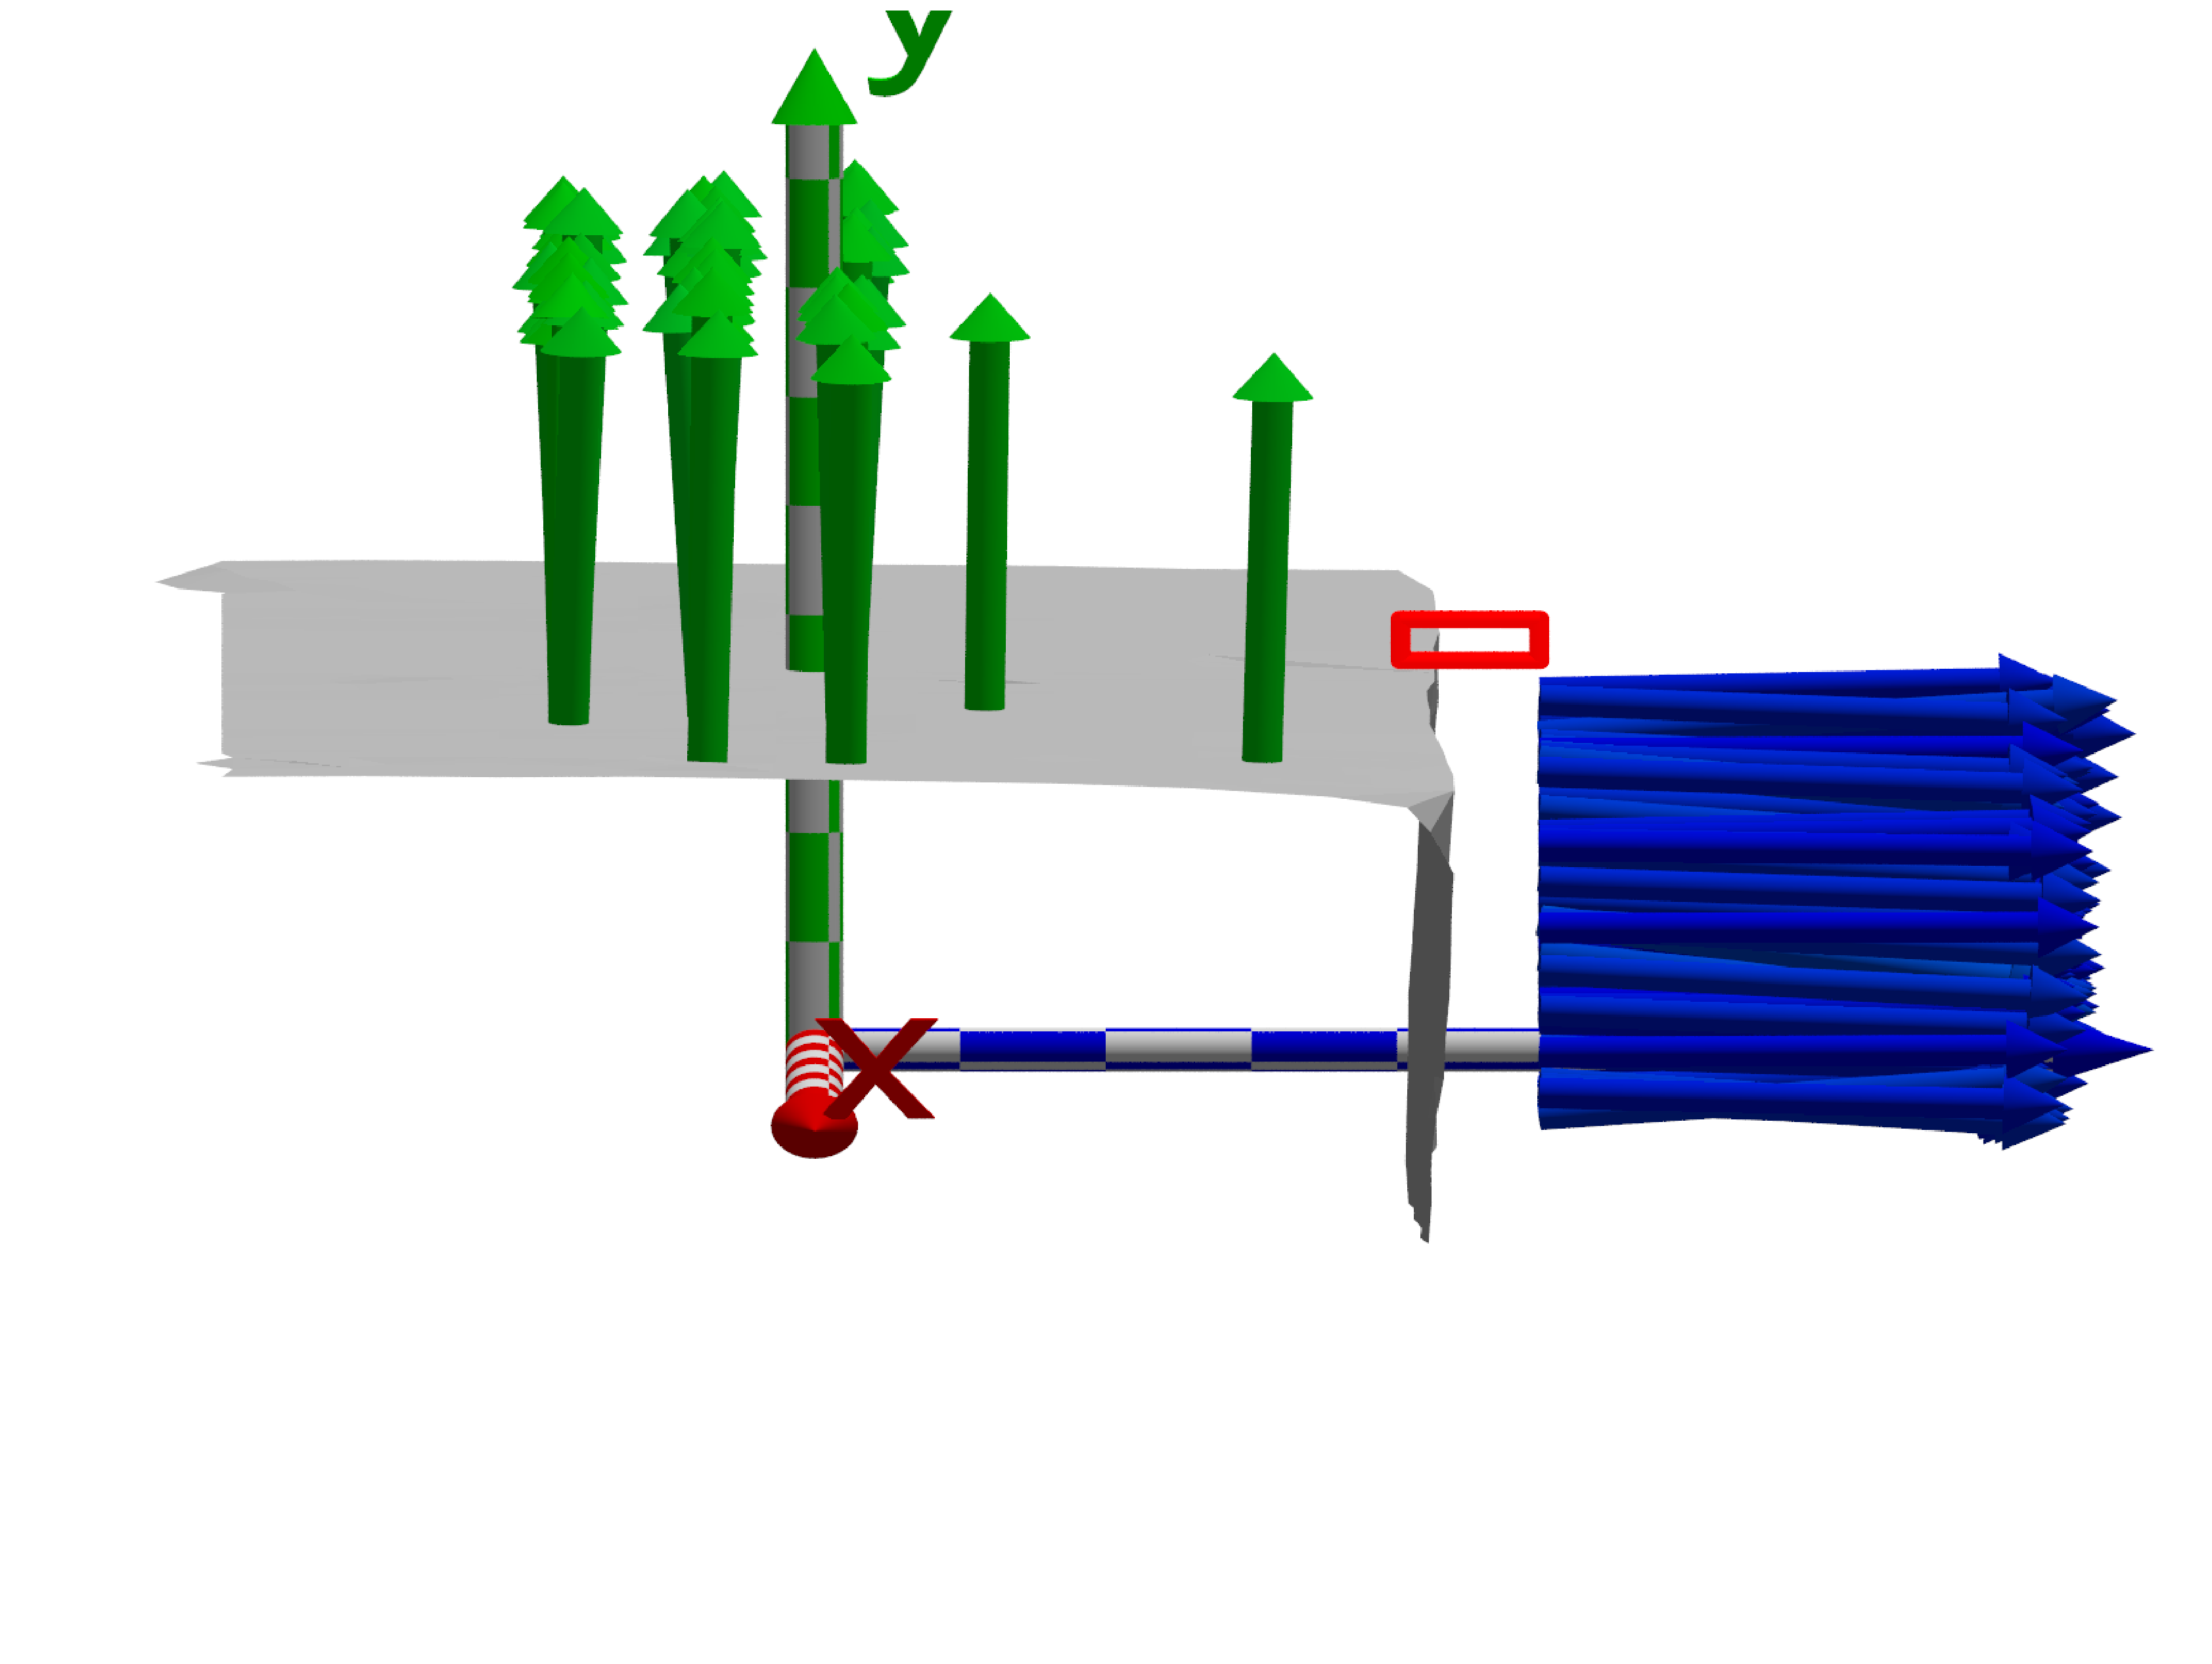
\includegraphics[width=0.25\linewidth]
             {images/setA.crop2.findReliable.new.eps}\label{fig:setA.crop1.findReliable}}
     \subfloat[ReliGrad]{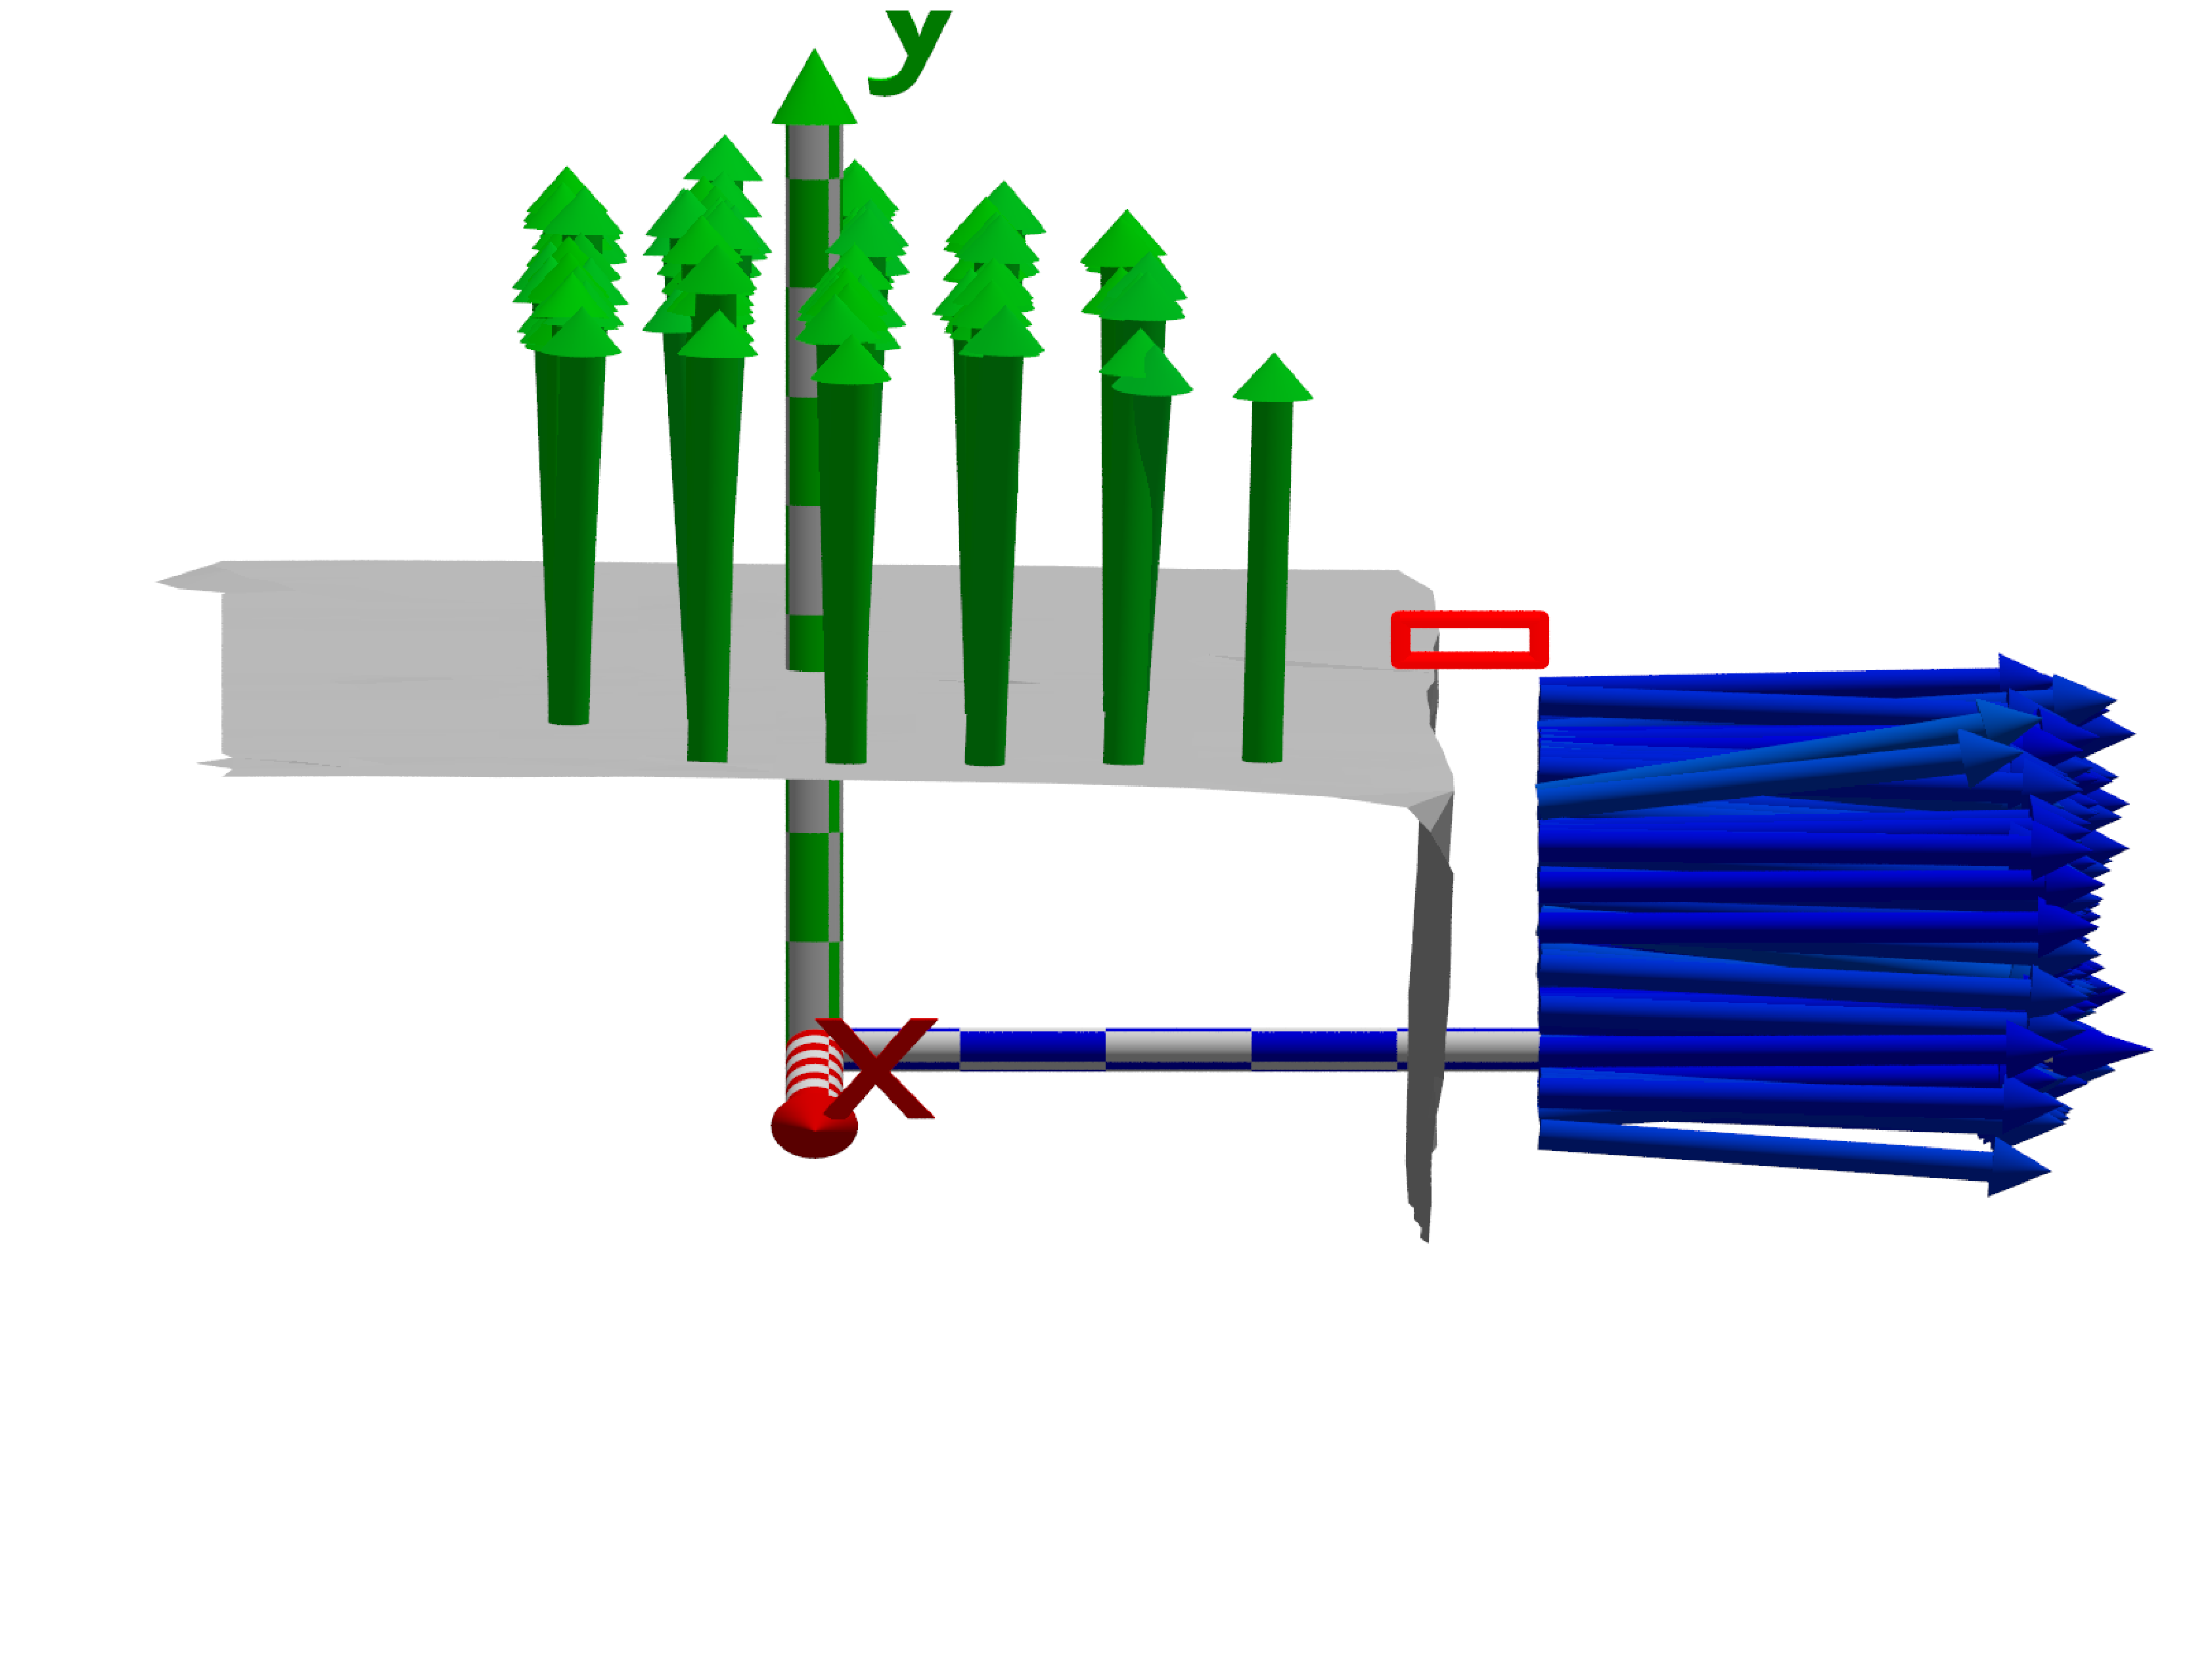
\includegraphics[width=0.25\linewidth]
                 {images/setA.crop2.religrad.new.eps}\label{fig:setA.crop1.religrad}}
\caption{The gradients generated on a portion of the \textit{engine cylinder} dataset.
The red rectangle shows the size of a grid cube
with spacing (0.27, 0.27, 0.68).
(a) Gradients marked reliable by Algorithm~\ref{alg:curved}. 
(b) Gradients marked reliable by Algorithm~\ref{alg:phi2}.
(c) Gradients marked reliable by \protect\FindReliable 
(Algorithm~\ref{alg:phi3}). 
(d) Gradients marked reliable by \protect\ReliGrad.}
\label{fig:setA.crop1.grads}
\end{figure}

% Please add the following required packages to your document preamble:
% \usepackage{multirow}
We also evaluate our algorithm on a number of industrial CT data sets (table~\ref{table:ictDataInfo}). 

\textbf{Description:} 
The \emph{CMM} dataset is a CT 
of solid alumimum shape used to calibrate CT devices.
\emph{CMM} stands for ``coordinate measuring machine''.
Figure~\subref*{fig:CMM:b} shows an isosurface from this data set.
Figure~\subref*{fig:CMM:a} shows a single slice along the XY plane. 
The \textit{Engine Cylinder} dataset is the CT 
of two motorcycle engine cylinders.
Figure~\subref*{fig:setA.crop1.1} shows a single slice
in an XY plane.
The slice exhibits streaking artifacts caused by beam hardening.
The \emph{Intake} dataset is a CT of a motorcycle engine intake valve.
Figure~\subref*{fig:intake:b} shows an isosurface of dataset, 
along with a single slice in an XY plane.
The \emph{Socket} dataset is a CT of 440 volt converter.
Figure~\subref*{fig:socket:c} shows a single
slice in the YZ plane using the hsv color scale. 
Table~\ref{table:ictDataInfo} provides the size and spacing
info on all these data sets.

\begin{figure}[htb]
    \centering
    \subfloat[Single image slice, original machine part]{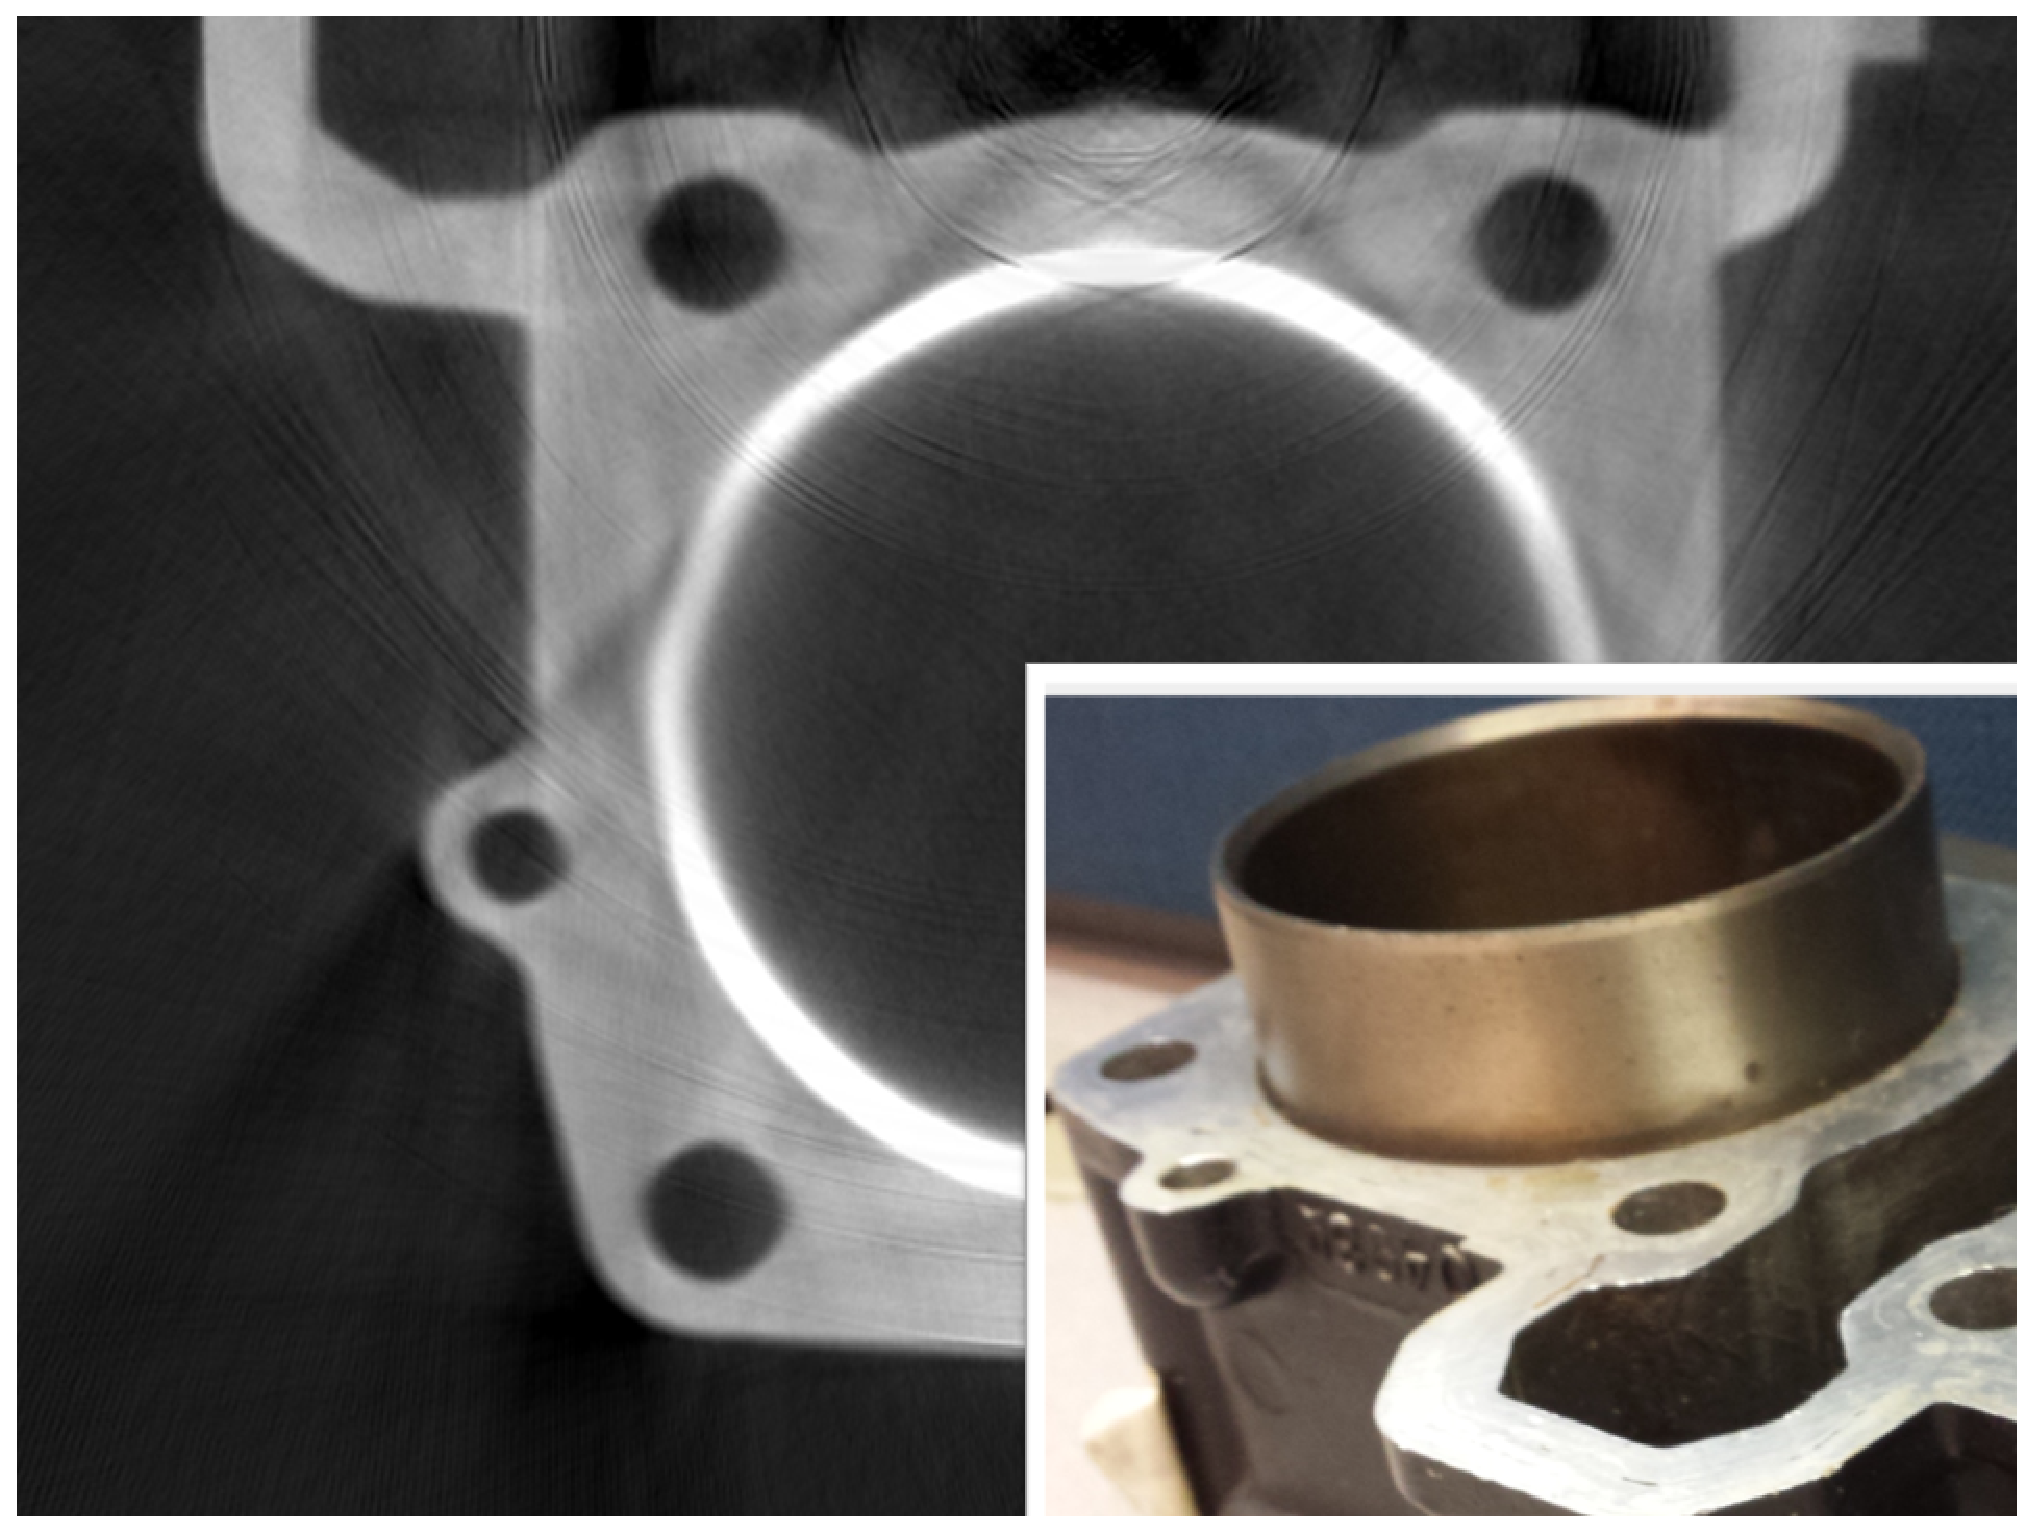
\includegraphics[width=0.3\linewidth ]{images/cly_sleeve.1.eps}\label{fig:setA.crop1.1}}
    \subfloat[Sharp Isosurface]{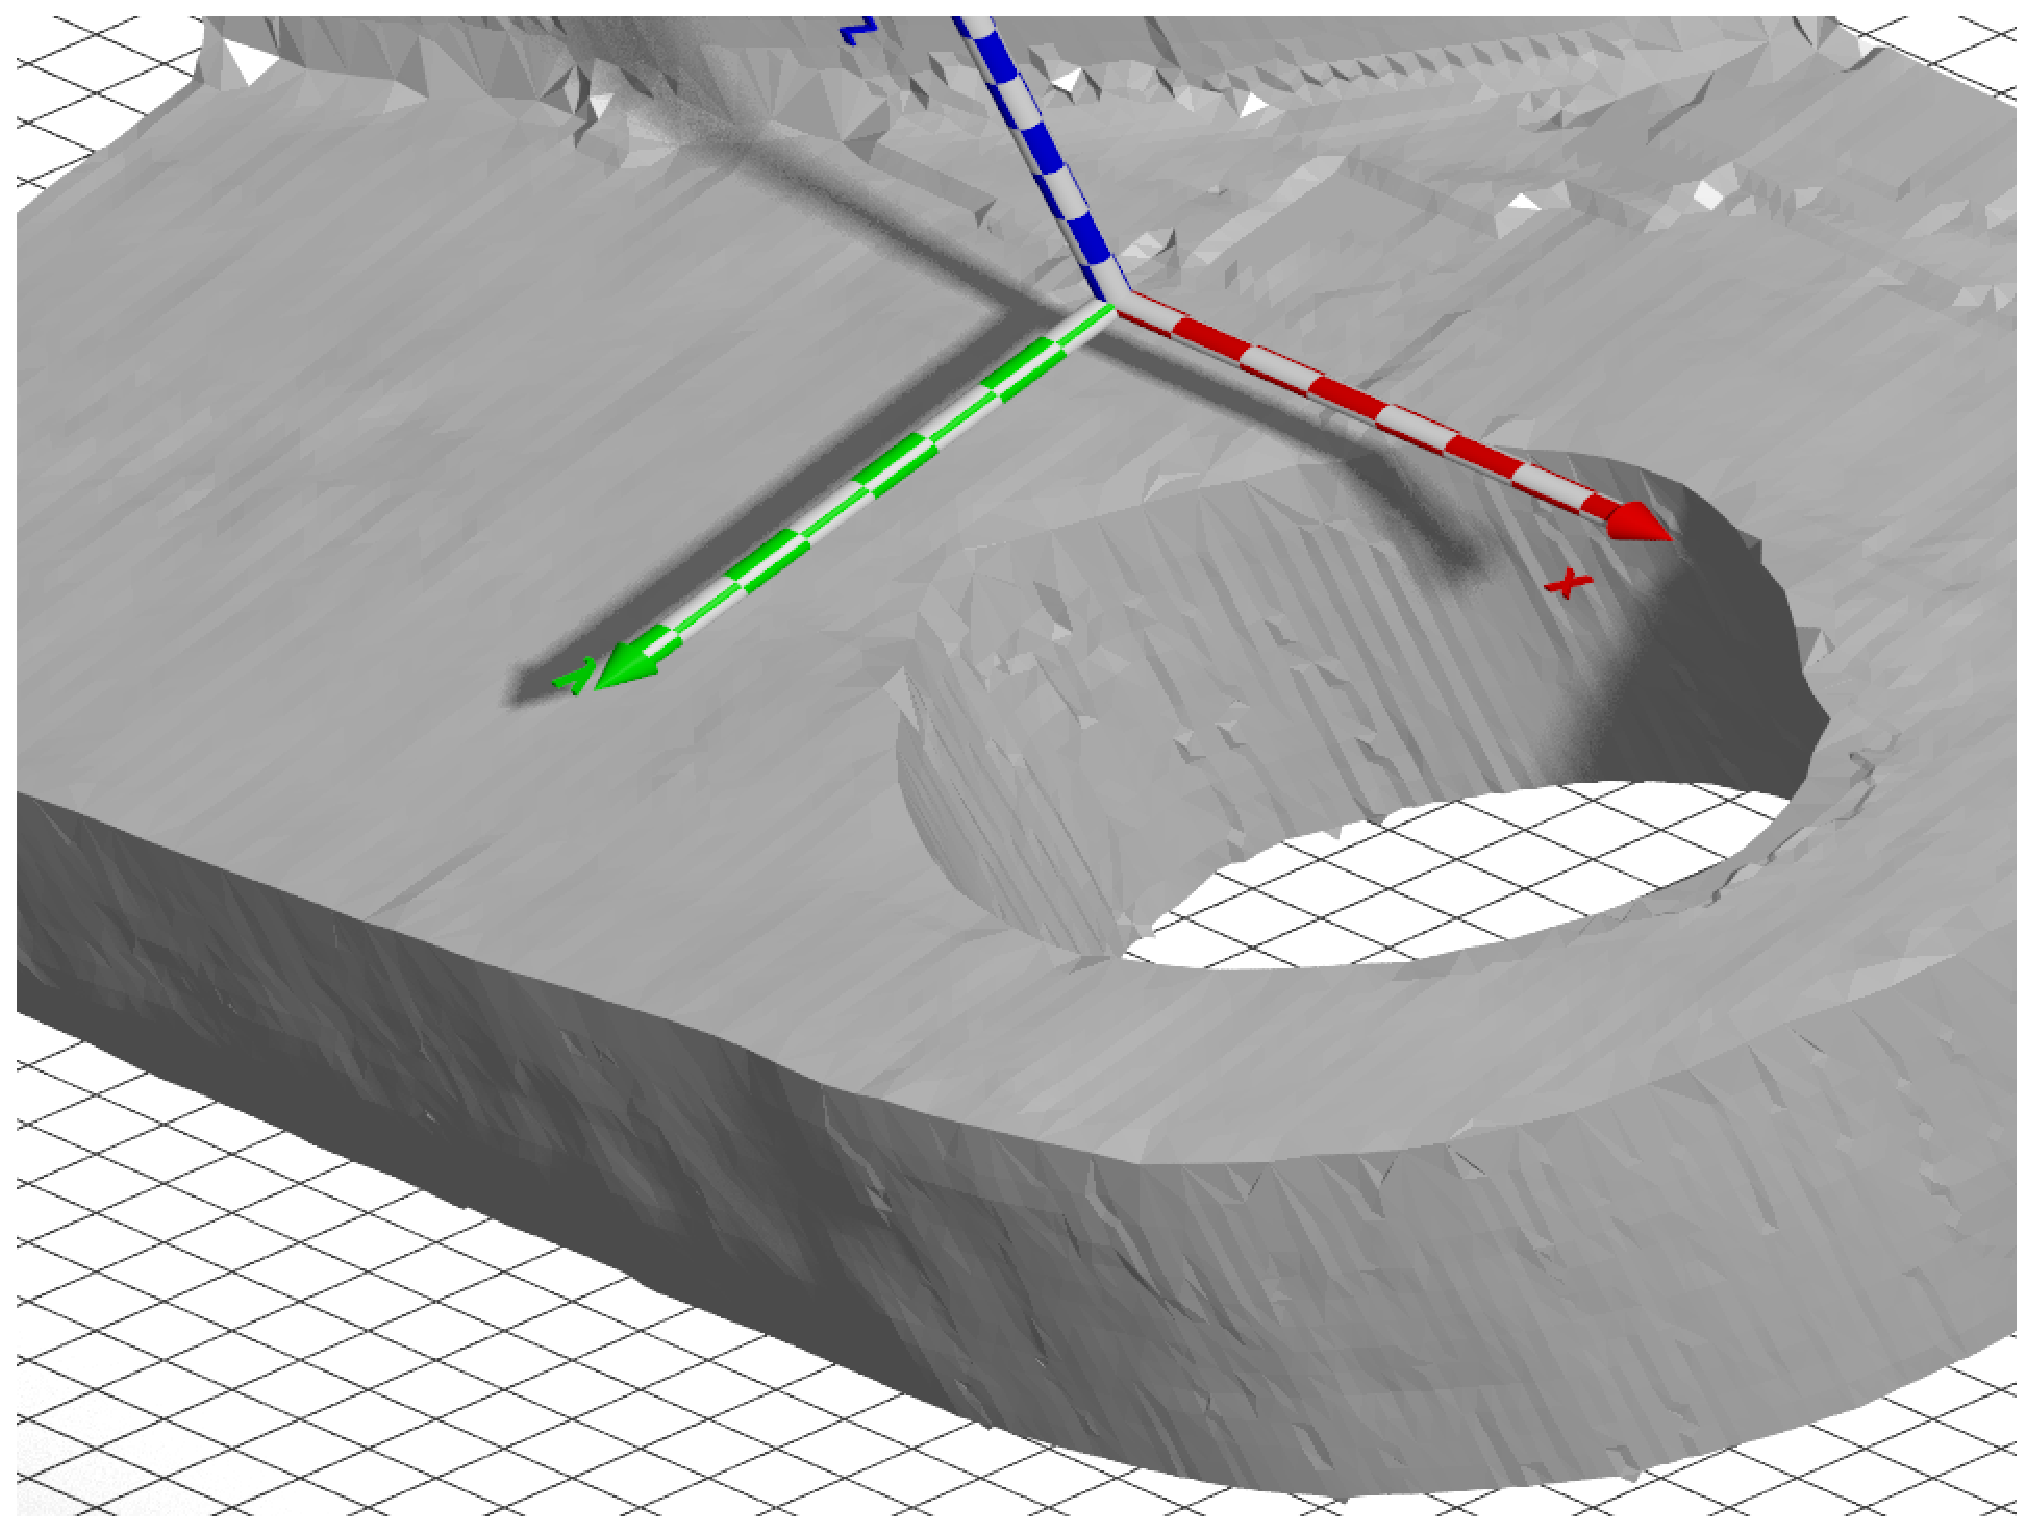
\includegraphics[width=0.3\linewidth]
        {images/setA.rendering.eps}\label{fig:setA.crop1.2}}
    \subfloat[Sparse feature points]{\includegraphics[width=0.3\linewidth]
        {images/setA.rendering2.eps}\label{fig:setA.crop1.3}}
    \caption{\textit{Engine Cylinder} dataset.~\protect\subref{fig:setA.crop1.1} a slice of the original CT image, note the streaking artifacts introduced during the scanning process.
    The inset shows the original machine part. Figure \protect\subref{fig:setA.crop1.2},~\protect\subref{fig:setA.crop1.3}, shows the sharp mesh, and the extracted sparse feature points.}
    \label{fig:setA.crop1}
\end{figure}

\textbf{Reliable Gradients} 
Figure~\ref{fig:setA.crop1.cdiff} shows the central difference gradients at all grid vertex location around an edge of the \textit{engine cylinder} dataset.
The length of the vectors are proportional to the magnitude of the gradients. Note that the gradients quickly fall off away from the isosurface. 
The problem is more severe along the Z-Axis. 
The magnified portion shows that there are about two good columns of gradients after which the gradient magnitude becomes too small and the gradient directions meaningless. 
Figure~\subref*{fig:setA.crop1.algo1},~\subref*{fig:setA.crop1.algo2} show the results of Algorithm ~\ref{alg:curved} and Algorithm ~\ref{alg:phi2} respectively. Unlike the simulated datasets, almost no gradients along the Z axis are marked as reliable. This shows the need for dividing the vertex set into tangential and orthogonal neighbor sets. This lead us to Algorithm~\ref{alg:religrad}. Figure~\subref*{fig:setA.crop1.findReliable} shows the corresponding gradients of the \FindReliable technique. Figure~\subref*{fig:setA.crop1.religrad} shows the~\ReliGrad gradients. For reference, Figure~\ref{fig:grad-1} shows the Central Difference gradients. 
  
\subsection{Visualization}
\subsubsection{Sparse feature point detection}
\label{sec:sparsePointExtraction}

From the reliable gradients, we can select a subset in the neighborhood of each cube (Section~\ref{sec:grad_select}),
compute points on the sharp features (Section~\ref{sec:computeSharpPoints}),
and select a well-spaced subset 
of those points (Section~\ref{sec:select_sharp}).

Figure~\subref*{fig:setA.crop1.mesh.2} shows the points on
a portion of the \textit{ engine cylinder} dataset.  
Figure~\subref*{fig:setA.crop1.mesh.3} shows a well-spaced subset 
of those points.

\subsubsection{Point Skeleton Visualization}
The sparse feature vertices are used to create a sharp feature point skeleton. The point set skeleton is visualized for the synthetic dataset in Figure~\ref{fig:SynData}. The number of large Eigenvalues determines if the sharp feature is on an edge or on a corner. Points on the edges are marked in green and corner points in red.
The skeleton is correctly extracted on challenging non-axis aligned datasets. We also do well on  acute and obtuse angles (Figure~\subref*{fig:cannon},~\subref*{fig:cone}).

Figure~\subref*{fig:setA.crop1.3} shows the extracted sparse point skeleton of a part of the \emph{engine cylinder} dataset. Figure~\subref*{fig:CMM:c} shows the point skeleton the CMM dataset. Figure~\subref*{fig:socket:b} shows the point skeleton of the \emph{socket} dataset.

 \begin{figure}
    \centering
    \subfloat[Annulus]{\includegraphics[width=0.3\linewidth]{images/volren.ann.eps}\label{fig:paraview:a}}
    \subfloat[Twocube]{\includegraphics[width=0.3\linewidth]{images/volren.twocube.eps}\label{fig:paraview:b}}\vspace {-3mm}
    \caption{Integrating results into ParaView~\cite{Ayachit2015}. Volume rendering of the Annulus and TwoCube dataset, overlayed with sparse feature skeleton.}
    \label{fig:paraview}
\end{figure}

%\begin{figure}[h]
%    \centering
%    \subfloat[Annulus]{\includegraphics[width=0.3\linewidth]{images/volren.ann.eps}\label{fig:paraview:a}}
%    \subfloat[Twocube]{\includegraphics[width=0.3\linewidth]{images/volren.twocube.eps}\label{fig:paraview:b}}
%    \caption{Integrating results into ParaView~\cite{Ayachit2015}. Volume rendering of the Annulus and TwoCube dataset, overlay-ed with sparse feature skeleton.}
%    \label{fig:paraview}
%\end{figure}
%
Apart from direct point visualization,  The extracted feature points can be quickly integrated into commonly used frameworks. For example, Figure~\subref*{fig:paraview:a},~\subref*{fig:paraview:b} shows the volume rendering of the datasets using ParaView~\cite{Ayachit2015}, overlay-ed  with the detected edge and corner points. The simple addition of the edge points makes the rendering more comprehensible.

\begin{figure}
    \centering
    \subfloat[Single XY slice, hsv color scale. Intensity range is 0-41000]{\includegraphics[width=0.3\linewidth]{images/CMM.singleSliceXY.eps}\label{fig:CMM:a}}
    \subfloat[MergeSharp Surface]{\includegraphics[width=0.3\linewidth]{images/CMM.full2.eps}\label{fig:CMM:b}}
%    \subfloat[Close Up of red square]{\includegraphics[width=0.3\linewidth]{images/CMM.close1.eps}\label{fig:CMM:c}}\hspace{1mm}
    \subfloat[Close Up of red square]{\includegraphics[width=0.3\linewidth]{images/CMM.close2.eps}\label{fig:CMM:c}}
    \caption{CMM dataset,~\protect\subref{fig:CMM:a} single slice XY plane.~\protect\subref{fig:CMM:b} MergeSharp isosurface.~\protect\subref{fig:CMM:c}  magnified red rectangle. Table~\ref{table:ictDataInfo} provides size and spacing.}
\end{figure}

\begin{figure}[tb]
    \centering
    \subfloat[Socket]{ \includegraphics[width=0.3\linewidth]{images/160uCT.1a.eps}\label{fig:socket:a} }
    \subfloat[Socket Close-up]{  \includegraphics[width=0.3\linewidth]{images/160uCT.2.eps}\label{fig:socket:b} }   
    \subfloat[XY Slice]{  \includegraphics[width=0.3\linewidth]{images/singleSlice.eps}\label{fig:socket:c} }   
    \caption{ (a) sharp mesh of a part of the \textit{socket} dataset. 
        (b) Close up. Corners are marked in red, sparse selected edge vertices are marked in green. (c) XY slice (hsv color scale, ParaView).}
    \label{fig:socket}
\end{figure}

\subsection{\mbox{Isosurface Reconstruction}}

The point skeleton generated by our algorithm can be input to mesh generation algorithms
to construct an isosurface mesh.
All the meshes  in Figure~\ref{fig:SynData} are generated using \MergeSharp applied
to the sharp points from our algorithm.
Figure~\ref{fig:setA.crop1.2} shows the extracted isosurface of a part of the \emph{engine cylinder} dataset.
  Figure~\subref*{fig:CMM:b} shows the isosurface generated from the CMM data set. Figure~\subref*{fig:CMM:c} shows close up of the red rectangle in Figure~\ref{fig:CMM:b}. The corner vertices are marked in red and the sparse edge vertices are marked in green. Figure~\subref*{fig:socket:a},~\subref*{fig:socket:b} shows an extracted isosurface of the socket dataset. Figure~\subref*{fig:intake:a} shows a \MergeSharp extracted mesh along with the sparse feature point skeleton of the \emph{intake} dataset.

The algorithm, WeightedCocone, by Dey et al.~\cite{dgqsww-fprss-12} constructs a surface mesh
from a point cloud which includes as input an identified set of points on sharp features.
We applied WeightedCocone on the point skeleton from the flange dataset.
We also supplied sample points on the smooth parts of the surface.
Figure~\subref*{fig:weightCocone} shows the sparse point skeleton and the resulting surface.
Other techniques which take as input feature curves/point can also
potentially use our results.

\subsection{Parameters}
Algorithm~\ReliGrad  has three parameters.
Among these $\alpha_{2}$ is the major parameter. 
$\alpha_{2}$ is a bound on the error in our prediction of a gradient 
at a grid vertex against the actual gradient at the vertex location. 
This includes the inherent noise in the data and the change in curvature.
\tiny
\begin{table}[h]
    \begin{tabular}{|l|l|l|l|l|}
        \hline
        \multirow{2}{*}{\begin{tabular}[c]{@{}l@{}}$\alpha_{2}$\\ in $^{\circ}$\end{tabular}} & \multicolumn{2}{l|}{Flange}                                                                                                & \multicolumn{2}{l|}{TwoCube}                                                    \\ \cline{2-5} 
        & \begin{tabular}[c]{@{}l@{}}MaxAngleDiff\\ in $^\circ$s\end{tabular} & \begin{tabular}[c]{@{}l@{}}Dist\\ 2Grad\end{tabular} & MaxAngleDiffin $^\circ$s & \begin{tabular}[c]{@{}l@{}}Dist\\ 2Grad\end{tabular} \\ \hline
        5                                                                                     & 4.11                                                                & 5                                                    & 3.3                      & 5                                                    \\ \hline
        10                                                                                    & 9.8                                                                 & 5                                                    & 8.0                      & 5                                                    \\ \hline
        15                                                                                    & 14.2                                                                & 4                                                    & 14.4                     & 4                                                    \\ \hline
        20                                                                                    & 19.7                                                                & 4                                                    & 19.2                     & 3                                                    \\ \hline
        25                                                                                    & 21.9                                                               & 4                                                    & 37.3                    & 3                                                    \\ \hline
        30                                                                                    & 25.0                                                               & 4                                                    & 73.1                    & 3                                                    \\ \hline
    \end{tabular}
    \caption{Effect of changing parameter $\alpha_{2}$ in \protect\ReliGrad.}
    \label{table:parameter}
\end{table}
\normalsize
Table~\ref{table:parameter} shows the effect of changing $\alpha_{2}$ on maxAngleDiff and Dist2Grad on the \textit{flange} and \textit{TwoCube} dataset. As expected, the maximum angle difference to the known correct gradients increases with increasing $\alpha_{2}$. While the maximum angle is 73.1 degrees, for \textit{TwoCube} with $\alpha_{2}$ set to 30 degrees, there were only 2 vertices with angle greater than 30 degrees. The \MergeSharp reconstruction showed no visible errors. 
 $\alpha_{1}$ decides if gradients at two vertices agree with each other. This is a much tighter threshold. For all our experiments this was set to 5$^{\circ}$s. We also always fixed the numIter, which decides how many times the reliable gradients are extended to 2, for all our tests. 
 The time to run the algorithm on all the datasets is in seconds. 
\begin{figure}
    \centering
    \subfloat[intake valve]{ \includegraphics[width=0.32\linewidth]{images/intake.1.crop.eps}\label{fig:intake:a} }
    \subfloat[Slice]{ \includegraphics[width=0.32\linewidth]{images/intake.sliceYZ.eps}\label{fig:intake:b} }
    \subfloat[Context]{ \includegraphics[width=0.32\linewidth]{images/intake.context.sliceYZ.eps}\label{fig:intake:c} }
    \caption{(a) sharp surface and point skeleton of the socket dataset. (b) a single slice of the YZ axis using the hsv color scale. (c) the slice along with the dataset, to provide context.}
    \label{fig:intake}
\end{figure}
 \begin{figure}[htb]
     \centering
      \subfloat[]{\includegraphics[width=0.33\linewidth]{images/cocone.result.eps} \label{fig:weightCocone}}
%     \subfloat[]{\includegraphics[width=0.33\linewidth]{images/fandisk.eps}
%         \label{fig:rimls}}
     \subfloat[]{\includegraphics[width=0.33\linewidth]{images/3dscan.new.eps}
     \label{fig:3dprint}}
     \caption{ ~\protect\subref*{fig:weightCocone} shows the result of SingularCocone using the sparse selected vertices as input and the corresponding output mesh on the Flange dataset.
%         Figure~\ref{fig:rimls} shows the result of running RIMLS~\cite{Oeztireli2009}, on a point dataset containing an edge and a corner, the edges are "pinched" not actually sharp. 
          Figure~\protect\subref*{fig:3dprint} shows a 3D print of Figure~\protect\subref*{fig:setA.crop1.2}.
}
     \label{fig:fandisk}
    \end{figure}
    
\section{Conclusion}

We showed that sharp features can be extracted directly 
from industrial CT scalar data, without extra information.
This is a major improvement over previous algorithms which require
exact surface normals or gradients.
We stress on this being a complete framework, starting directly from the CT scan, to constructing isosurface meshes with good representation of sharp edges and corners. 
Figure~\subref*{fig:3dprint} shows a 3D printing of a part of the \emph{cylinder engine} dataset from the  mesh extracted in Figure~\subref*{fig:setA.crop1.2}.


\bibliographystyle{abbrv}
%%use following if all content of bibtex file should be shown
%\nocite{*}
\bibliography{religradTR}

\appendix
\newpage


% Environments for repeating propositions.
\newtheorem*{propAngle}{Proposition \ref{prop:angle}}
\newtheorem*{propAngle:b}{Proposition \ref{prop:angle:b}}
\newtheorem*{propIV}{Proposition \ref{prop:IV}}
\newtheorem*{propkappa}{Proposition \ref{prop:kappa}}
\newtheorem*{propIVb}{Proposition \ref{prop:IV:b}}


\begin{figure}[t]
\begin{center}
\begin{tabular}{cc}
\includegraphics[width=1.2in]{images/phiTriangles.eps} \quad &
\quad
\includegraphics[width=1.2in]{images/phiDiff2.eps} \\
(a) & (b)
\end{tabular}
\end{center}
\caption{
(a) Triangles $\Delta_1$, $\Delta_2$, $\Delta''_1$ and $\Delta''_2$.
(b) Rotating $n$ and $\tn'$ around line $L$.}
\label{fig:triangles}
\end{figure}

\section{Proofs}

\subsection{Angle Lemmas}

Let $n$ and $n'$ be unit vectors in $\Rthree$.
Recall the following definitions, from Section~\ref{sec:reliable}.
\begin{align*}
\Orth(n,n') & = n - (n \cdot n') n' \\ 
\phi(n,n') & = n - 2 \times \Orth(n,n') = 2(n \cdot n') n' - n.
\end{align*}
Vector $\Orth(n,n')$ is the component of $n$ orthogonal to $n$.
Vector $\phi(n,n')$ is the vector 
{\em predicted by} $n$ and $n'$.

\begin{align*}
\cos(\angle(\phi(n,n'),n')) & = (2 (n \cdot n') n' -n) \cdot n' \\
  & = 2 (n \cdot n') (n' \cdot n') - (n \cdot n') \\
  & = 2 (n \cdot n') - (n \cdot n') \mbox{  (since $n'$ is a unit vector)} \\
  & = n \cdot n' = \cos(\angle(n,n')).
\end{align*}
Thus, $\angle(\phi(n,n'),n')$ equals $\angle(n,n')$.

\begin{lemma}
If $n$, $n'$ and $n''$ are unit vectors, then
\begin{enumerate}
\item $\Lambda(n,n',n'') = \Lambda(n'',n',n)$, and
\item $\angle(n,n'') = \angle(\phi(n,n'),\phi(n'',n'))$.
\end{enumerate}
\label{lemma:phi}
\end{lemma}

\begin{proof}
Let $\OO$ be the origin $(0,0,0)$.
Let $\Delta_1$, $\Delta_2$, $\Delta''_1$ and $\Delta''_2$
be the triangles $\Delta(\OO,n',n)$, $\Delta(\OO,n',\phi(n,n'))$,
$\Delta(\OO,n',n'')$ and $\Delta(\OO,n',\phi(n'',n'))$, respectively.
(See Figure~\ref{fig:triangles}.(a).)

As noted above, $\angle(n,n')$ equals $\angle(\phi(n,n'),n')$.
Similarly, $\angle(n',n'')$ equals $\angle(\phi(n'',n'), n')$.
Since $n$, $n'$ and  $\phi(n,n')$ have the same (unit) length,
triangles $\Delta_1$ and $\Delta_2$ are congruent.
Since $n'$, $n''$ and  $\phi(n'',n')$ have the same (unit) length,
triangles $\Delta''_1$ and $\Delta''_2$ are congruent.

Since $n$, $n'$ and $\phi(n,n')$ are co-planar
and $n''$, $n'$ and $\phi(n'',n')$ are co-planar,
the dihedral angles between $\Delta_1$ and $\Delta''_2$ 
equals the dihedral angle between $\Delta_2$ and $\Delta''_1$.
Thus, tetrahedron $(\OO,n,n',\phi(n'',n'))$ is congruent
to tetrahedron $(\OO,n',n'',\phi(n,n'))$
and $\angle(n, \phi(n'',n'))$ equals $\angle(n'', \phi(n,n'))$
and $\angle(n,n'')$ equals $\angle(\phi(n,n'),\phi(n'',n'))$.
\end{proof}

The following corollary describes how $\angle(\phi(n,n'))$
and $\Lambda(n,n',n'')$ change when unit vector $n$ is replaced by $\tn$.
\begin{corollary}
If $n$, $\tn$, $n'$ and $n''$ are unit vectors
and $\angle(n,\tn) \le \mu$, then
\begin{enumerate}
\item $\angle(\phi(n,n'),\phi(\tn,n')) \le \mu$;
\item $|\Lambda(n,n',n'') - \Lambda(\tn,n',n'')| \le \mu$.
\end{enumerate}
\label{corollary:phi}
\end{corollary}

\begin{proof}
By Lemma~\ref{lemma:phi},
angle $\angle(n,\tn)$ equals $\angle(\phi(n,n'), \phi(\tn,n'))$.
(Let $n''$ represent $\tn$ in Lemma~\ref{lemma:phi}.)
Thus,
\begin{align*}
\angle(\phi(n,n'),\phi(\tn,n')) & = \angle(n,\tn) \le \mu, \qquad \mbox{and} \\
|\Lambda(n,n',n'') - \Lambda(\tn,n',n'')| & = 
|\angle(\phi(n,n'),n'') - \angle(\phi(\tn,n'),n'')|  \\
  & \le \angle(\phi(n,n'),\phi(\tn,n')) \le \mu.
\end{align*}
\end{proof}

In the following corollary,
vector $n'$ is replaced by $\tn'$.
The bounds are slightly different than the bounds in the previous corollary.
\begin{corollary}
If $n$, $n'$, $\tn'$, $n''$ and $n'''$ are unit vectors
and $\angle(n',\tn') \le \mu$ and $\angle(\phi(n,n'),n'') \le \gamma$, 
then
\begin{enumerate}
\item $\angle(\phi(n,n'),\phi(n,\tn')) \le 2\mu$;
\item $|\Lambda(n,n',n'') - \Lambda(n,\tn',n'')| \le 2\mu$;
\item $|\Lambda(n',n'',n''') - \Lambda(n',\phi(n,n'),n''') \le 2\gamma$.
\end{enumerate}
\label{corollary:phi:2}
\end{corollary}

\begin{proof}
Let $L$ be the line through the origin orthogonal to $n'$ and $\tn'$.
Rotating $\tn'$ and $n$ by angle $\angle(\tn',n')$ around $L$
maps $\tn'$ to $n'$ and $n$ to a unit vector $\tn$
where $\angle(n,\tn) \le \mu$ (Figure~\ref{fig:triangles}.(b).)
By Corollary~\ref{corollary:phi},
$\angle(\phi(n,n'),\phi(\tn,n')) \le \mu$.
Rotating $\tn$, $n'$ and $\phi(\tn,n')$ by angle $-\angle(\tn',n')$ around $L$
maps $\tn$ back to $n$, vector $n'$ to $\tn'$ and $\phi(\tn,n')$
to $\phi(n,\tn')$.
Since $|-\angle(\tn',n')| \le \mu$,
angle $\angle(\phi(\tn,n'),\phi(n,\tn')) \le \mu$.
Thus,
\begin{align*}
\angle(\phi(n,n'),\phi(n,\tn')) 
 & \le \angle(\phi(n,n'),\phi(\tn,n')) + \angle(\phi(\tn,n'),\phi(n,\tn')) \\
 & \le 2 \mu,
\end{align*}
and
\begin{align*}
|\Lambda(n,n',n'') - \Lambda(n,\tn',n'')| & = 
|\angle(n'', \phi(n,n')) - \angle(n'', \phi(n,\tn'))|  \\
  & \le \angle(\phi(n,n'),\phi(n,\tn')) \le 2\mu.
\end{align*}

Replacing $n$, $n'$, $\tn'$, $n''$ and $\mu$
by $n'$, $n''$, $\phi(n,n')$, $n'''$ and $\gamma$ in the formula above,
gives
\begin{align*}
|\Lambda(n',n'',n''') - \Lambda(n',\phi(n,n'),n''')| \le 2 \gamma.
\end{align*}

\end{proof}

\begin{lemma}
If $n$, $n'$ and $n''$ are unit vectors, then
\begin{enumerate}
\item $\phi_2(n,n') = \phi_1(n',\phi_1(n,n')$, and
\item $\Lambda_2(n,n',n'') = \Lambda_1(n', \phi_1(n,n'), n''))$.
\end{enumerate}
\label{lemma:Lambda2}
\end{lemma}

\begin{proof}

By definition,
\begin{align*}
\phi_2(n,n') = \phi_1(\phi_0(n,n'), \phi_1(n,n')) = \phi_1(n', \phi_1(n,n')).
\end{align*}

Thus,
\begin{align*}
\Lambda_2(n,n',n'') & = \angle(\phi_2(n,n'),n'') \\
  & = \angle(\phi_1(n',\phi_1(n,n')), n'')  
    = \Lambda_1(n', \phi_1(n,n'), n'').
\end{align*}

\end{proof}

\begin{corollary}
If $n$, $n'$ and $n''$ are unit vectors
and $\angle(n,\tn) \le \mu$,
then $|\Lambda_2(n,n',n'') - \Lambda_2(\tn,n',n'')| \le 2\mu$.
\label{corollary:Lambda2}
\end{corollary}

\begin{proof}

By Lemma~\ref{lemma:phi},
\begin{align*}
\angle(\phi_1(n,n'),\phi_1(\tn,n')) = \angle(n,\tn) \le \mu.
\end{align*}

Thus,
\begin{align*}
\Lambda_2(n,n',n'') & = \Lambda_1(n', \phi(n,n'), n'') 
  & \mbox{(Lemma~\ref{lemma:Lambda2})} \\
& \le \Lambda_1(n', \phi(\tn,n'), n'') + 2\mu
  & \mbox{(Corollary~\ref{corollary:phi:2})} \\
& = \Lambda_2(\tn,n',n'') + 2 \mu.
\end{align*}

Swapping $n$ and $\tn$ gives
$\Lambda_2(\tn,n',n'') \le \Lambda_2(n, n',n'') + 2 \mu$.
Thus,
$|\Lambda_2(n,n',n'') - \Lambda_2(\tn, n',n'')| \le 2 \mu$.
\end{proof}

\begin{corollary}
If $n$, $n'$ and $n''$ are unit vectors
and $\angle(n',\tn') \le \mu$,
then $|\Lambda_2(n,n',n'') - \Lambda_2(n,\tn',n'')| \le 3\mu$.
\label{corollary:Lambda2:2}
\end{corollary}

\begin{proof}

By Lemma~\ref{lemma:phi},
\begin{align*}
\angle(\phi_1(n,n'),\phi_1(n,\tn')) = \angle(n',\tn') \le \mu.
\end{align*}

Thus,
\begin{align*}
\Lambda_2(n,n',n'') & = \Lambda_1(n', \phi(n,n'), n'') 
  & \mbox{(Lemma~\ref{lemma:Lambda2})} \\
& \le \Lambda_1(\tn', \phi(n,n'), n'') + \mu
  & \mbox{(Corollary~\ref{corollary:Lambda2})} \\
& \le \Lambda_1(\tn', \phi(n,\tn'), n'') + 2\mu + \mu
  & \mbox{(Corollary~\ref{corollary:phi:2})} \\
& = \Lambda_2(n,\tn',n'') + 3 \mu.
\end{align*}

Swapping $n'$ and $\tn'$ gives
$\Lambda_2(n,n',n'') \le \Lambda_2(n, \tn',n'') + 3 \mu$.
Thus,
$|\Lambda_2(n,\tn',n'') - \Lambda_2(n, \tn',n'')| \le 3 \mu$.

\end{proof}

\begin{corollary}
If $n$, $n'$, $n''$ and $n'''$ are unit vectors
and $\Lambda(n,n',n'') \le \gamma$
and $\Lambda(n',n'',n''') \le \gamma$,
then $\Lambda_2(n,n',n''') \le 3\gamma$.
\label{corollary:Lambda2:3}
\end{corollary}

\begin{proof}
By assumption, $\Lambda_1(n,n',n'') \le \gamma$,
so $\angle(\phi_1(n,n'),n'') \le \gamma$.
\begin{align*}
\Lambda_2(n,n',n''') & = \Lambda_1(n', \phi_1(n,n'), n'')
 & \mbox{(Lemma~\ref{lemma:Lambda2})} \\
 & \le \Lambda_1(n', n'', n''') + 2 \gamma 
 & \mbox{(Corollary~\ref{corollary:phi:2})} \\
 & \le 3\gamma.
\end{align*}
\end{proof}


\subsection{Angle bounds}

We now give bounds on $\Lambda$ and on the angles
between the exact and approximated normals.

\begin{propAngle}
Let $(v, v', v'')$ be a collinear sequence of adjacent vertices
contained in $A_i$ for some smooth region $A_i$.
\begin{enumerate}
\item If $v, v', v'' \in \IV(A_i)$, then\\
{\centering
$\Lambda(\tn_v, \tn_{v'}, \tn_{v''}) \le 
\Lambda(n_v, n_{v'}, n_{v''}) + 4 \mu \le \lambda + 4 \mu$.}
\item If $v, v' \in \IV(A_i)$, then
$\angle(n_{v''},\tn_{v''}) \le 
   \Lambda(\tn_v,\tn_{v'},\tn_{v''}) + 3 \mu + \lambda$.
\end{enumerate}
\end{propAngle}

\begin{proof}[Proof of \ref{prop:angle}.1]
Since $v$, $v'$ and $v''$ are interior vertices,
angles $\angle(n_v,\tn_v)$, $\angle(n_{v'}, \tn_{v'})$ 
and $\angle(n_{v''}, \tn_{v''})$ are all less than $\mu$.
\begin{align*}
\Lambda(\tn_v,\tn_{v'},\tn_{v''}) & \le \Lambda(\tn_v, \tn_{v'}, n_{v''}) + \mu 
    \\
  & \le \Lambda(n_v, \tn_{v'}, n_{v''}) + \mu + \mu 
    & \mbox{(Corollary~\ref{corollary:phi})} \\
  & \le \Lambda(n_v, n_{v'}, n_{v''}) + 2\mu + \mu + \mu 
    & \mbox{(Corollary~\ref{corollary:phi:2})} \\
  & = \Lambda(n_v, n_{v'}, n_{v''}) + 4 \mu \le \lambda + 4 \mu.
\end{align*}

\end{proof}

\begin{proof}[Proof of \ref{prop:angle}.2]

\begin{align*}
\angle(n_{v''},\tn_{v''}) & \le \angle(\phi(n_v,n_{v'}),n_{v''}) +
\angle(\phi(n_v,n_{v'}),\tn_{v''}) \\
& \le \lambda + \Lambda(n_v, n_{v'}, \tn_{v''}).
\end{align*}

Since $\angle(n_v,\tn_v) \le \mu$,
\begin{align*}
\Lambda(n_v, n_{v'}, \tn_{v''}) & 
  \le \Lambda(\tn_v, n_{v'}, \tn_{v''}) + \mu.
& \mbox{(Corollary~\ref{corollary:phi})}
\end{align*}

Since $\angle(n_{v'},\tn_{v'}) \le \mu$,
\begin{align*}
\Lambda(\tn_v, n_{v'}, \tn_{v''}) & 
\le \Lambda(\tn_v, \tn_{v'}, \tn_{v''}) + 2\mu.
& \mbox{(Corollary~\ref{corollary:phi:2})}
\end{align*}

Thus,
\begin{align*}
\Lambda(n_v, n_{v'}, \tn_{v''}) & \le \Lambda(\tn_v, n_{v'}, \tn_{v''}) + \mu
\le \Lambda(\tn_v, \tn_{v'}, \tn_{v''}) + 3\mu, \mbox{ and} \\
\angle(n_{v''},\tn_{v''}) & \le \lambda + \Lambda(n_v, n_{v'}, \tn_{v''})
  \le \lambda + \Lambda(\tn_v, \tn_{v'}, \tn_{v''}) + 3\mu \\
& = \Lambda(\tn_v, \tn_{v'}, \tn_{v''}) + 3\mu+ \lambda.
\end{align*}

\end{proof}

The following corollary follows directly from Proposition~\ref{prop:angle}.1.
\begin{corollary}
Let $(v,v',v'')$ be a collinear sequence of adjacent grid vertices
where vertices $v,v',v'' \in A_1$
and $v'$ and $v''$ are interior vertices in $A_1$.
If $\Lambda(\tn_v,\tn_{v'},\tn_{v''}) \le \alpha$, then
\begin{equation*}
\angle(n_{v''},\tn_{v''}) \le \alpha + 3 \mu + \lambda.
\end{equation*}
\label{corollary:collinear}
\end{corollary}

The proofs of Proposition~\ref{prop:angle:b} are similar
to the proofs of Proposition~\ref{prop:angle}.

\begin{propAngle:b}
Let $(v, v', v'',v''')$ be a collinear sequence of adjacent vertices
contained in $A_i$ for some smooth region $A_i$.
\begin{enumerate}
\item If $v, v', v'', v''' \in \IV(A_i)$, then\\
{\centering
$\Lambda_2(\tn_v, \tn_{v'}, \tn_{v'''}) \le 
\Lambda_2(n_v, n_{v'}, n_{v'''}) + 4 \mu \le 3\lambda + 6 \mu$.}
\item If $v, v' \in \IV(A_i)$, then\\
{\centering
$\angle(n_{v'''},\tn_{v'''}) 
   \le \Lambda(\tn_v,\tn_{v'},\tn_{v'''}) + 3\lambda+ 5 \mu$.}
\end{enumerate}
\end{propAngle:b}

\begin{proof}[Proof of~\ref{prop:angle:b}.1]

Since $v$, $v'$, $v''$ and $v'''$ are interior vertices,
angles $\angle(n_v,\tn_v)$, $\angle(n_{v'}, \tn_{v'})$,
$\angle(n_{v''}, \tn_{v''})$ and $\angle(n_{v'''},\tn_{v'''})$
are all less than $\mu$.
\begin{align*}
\Lambda_2(\tn_v,\tn_{v'},\tn_{v'''}) 
  & \le \Lambda_2(\tn_v, \tn_{v'}, n_{v'''}) + \mu \\
  & \le \Lambda_2(n_v, \tn_{v'}, n_{v'''}) + \mu + 2\mu 
    & \mbox{(Corollary~\ref{corollary:Lambda2})} \\
  & \le \Lambda_2(n_v, n_{v'}, n_{v'''}) + 3\mu + 2\mu + \mu 
    & \mbox{(Corollary~\ref{corollary:Lambda2:2})} \\
  & = \Lambda_2(n_v, n_{v'}, n_{v'''}) + 6 \mu \\
  & \le 3\lambda +  6 \mu.  
    & \mbox{(Corollary~\ref{corollary:Lambda2:3})}
\end{align*}

\end{proof}

\begin{proof}[Proof of~\ref{prop:angle:b}.2]

\begin{align*}
\angle(n_{v'''},\tn_{v'''}) 
  &  \le \angle(\phi_2(n_v, n_{v'}), n_{v'''}) 
         + \angle(\phi_2(n_v,n_{v'}), \tn_{v'''}) \\
  & = \Lambda_2(n_v, n_{v'}, n_{v'''}) 
      + \angle(\phi_2(n_v,n_{v'}), \tn_{v'''}) \\
  & \le 3 \lambda + \Lambda_2(n_v, n_{v'}, \tn_{v'''}).
  & \mbox{(Lemma~\ref{lemma:Lambda2})}
\end{align*}

Since $\angle(n_v,\tn_v) \le \mu$,
\begin{align*}
\Lambda_2(n_v, n_{v'}, \tn_{v'''}) 
  & \le \Lambda_2(\tn_v, n_{v'}, \tn_{v'''}) + 2\mu.
& \mbox{(Corollary~\ref{corollary:Lambda2})}
\end{align*}

Since $\angle(n_{v'},\tn_{v'}) \le \mu$,
\begin{align*}
\Lambda_2(\tn_v, n_{v'}, \tn_{v'''}) & 
\le \Lambda_2(\tn_v, \tn_{v'}, \tn_{v'''}) + 3\mu.
& \mbox{(Corollary~\ref{corollary:Lambda2:2})}
\end{align*}

Thus,
\begin{align*}
\Lambda_2(n_v, n_{v'}, \tn_{v'''}) 
   & \le \Lambda_2(\tn_v, n_{v'}, \tn_{v'''}) + 2\mu
\le \Lambda_2(\tn_v, \tn_{v'}, \tn_{v'''}) + 5\mu, \mbox{ and} \\
\angle(n_{v'''},\tn_{v'''}) & \le 3\lambda + \Lambda_2(n_v, n_{v'}, \tn_{v'''})
  \le 3\lambda + \Lambda_2(\tn_v, \tn_{v'}, \tn_{v'''}) + 5\mu \\
& = \Lambda_2(\tn_v, \tn_{v'}, \tn_{v'''}) + 3\lambda + 5 \mu.
\end{align*}

\end{proof}


We also give bounds on $\angle(\tn_v, \tn_{v'})$
and on  $\angle(n_{v'},\tn_{v'})$.
We first define a bound $\kappa$ on $\angle(n_v,n_{v'})$
in smooth regions of $f$.
\begin{align*}
\kappa = \max\{ \angle(n_v,n_{v'}) v,v' \in A_i \mbox{ for some } A_i \}.
\end{align*}
Value $\kappa$ can be viewed as a bound on the curvature of the field
within smooth regions.
In comparison, $\lambda$ is a bound on the change in curvature
of the field within smooth regions.

The following proposition gives bounds on $\angle(n_{v'},\tn_{v'})$
based on $\angle(\tn_v, \tn_{v'})$.
\begin{proposition}
Let $v$ and $v'$ be adjacent vertices contained in $A_i$
for some smooth region $A_i$.
\begin{enumerate}
\item If $v, v' \in \IV(A_i)$, then
$\angle(\tn_v, \tn_{v'}) \le \angle(n_v, \tn_{v'}) + 2 \mu \le \kappa + 2 \mu$.
\item If $v \in \IV(A_i)$, then
$\angle(n_{v'}, \tn_{v'}) \le \angle(\tn_v, \tn_{v'}) + \kappa + \mu$.
\end{enumerate}
\label{prop:kappa}
\end{proposition}

\begin{proof}[Proof of \ref{prop:kappa}.1.]
\begin{align*}
\angle(\tn_v,\tn_{v'}) & \le \angle(n_v, \tn_{v'}) + \angle(n_v, \tn_v)
              \le \angle(n_v, \tn_{v'}) + \mu \\
             & \le \angle(n_v, n_{v'}) + \angle(n_{v'}, \tn_{v'}) + \mu \\
             & \le \angle(n_v, n_{v'}) + \mu + \mu 
               = \angle(n_v,n_{v'}) + 2 \mu \le \kappa+ 2 \mu.
\end{align*}
\end{proof}


\begin{proof}[Proof of \ref{prop:kappa}.2.]
\begin{align*}
\angle(n_{v'},\tn_{v'}) & \le \angle(n_v,\tn_{v'}) + \angle(n_v, n_{v'})
  \le \angle(n_v,\tn_{v'}) + \kappa \\
& \le \angle(\tn_v, \tn_{v'}) + \angle(n_v,\tn_v) + \kappa
  \le \angle(\tn_v, \tn_{v'}) + \mu + \kappa.
\end{align*}
\end{proof}

\subsection{Containment bounds}

To prove Proposition~\ref{prop:IV},
we show that if a sufficiently large ball $\BB$ contains vertex $v$,
then $\BB$ contains $N(v'')$ and $N(v''')$
for some collinear sequence $(v,v',v'',v''')$.
\begin{lemma}
Let $\Gamma$ be a regular grid whose edges all have the same length $L$.
If some ball $\BB$ of radius $(5/2) \sqrt{3}L$ contains grid vertex $v$,
then there is a collinear sequence $(v,v',v'',v''')$ 
of adjacent grid vertices
such that $\BB$ contains $N(v'')$ and $N(v''')$.
\label{lemma:ball}
\end{lemma}

\begin{proof}
Let $\BB$ be a ball of radius $(5/2)\sqrt{3}L$ containing grid vertex $v$.
Let $q$ be the center of $\BB$.
Without loss of generality assume vertex $v$ is at the origin $(0,0,0)$,
that the edge length $L$ equals 1,
and that $q$ lies in the positive $x$, $y$ and $z$ orthant.
Let $D \le (5/2) \sqrt{3}$ be the distance from the origin to $q$.
The coordinates of $q$ can be expressed as $D(u_x,u_y,u_z)$
where $(u_x,u_y,u_z)$ is a unit vector.

Without loss of generality, assume that $q$ is closest to the $x$-axis,
i.e., $u_x \ge u_y$ and $u_x \ge u_z$.
Let $v''$ be $(2,0,0)$ and $v'''$ be $(3,0,0)$.
We claim that $N_{v''}$ and $N_{v'''}$ are in $\BB$.

Let $p$ be the grid vertex with coordinates $(3,-1,0)$.
Point $p$ is in $N_{v''}$.
Let $R$ equal $(5/2)\sqrt{3}$.
Since ball $\BB$ contains the origin,
distance $D$ is at most $R$.
\begin{align*}
|q-p|^2 & = (D u_x-3)^2 + (D u_y+1)^2 + (D u_z)^2 \\
 & = D^2 u_x^2 - 6 D u_x + 9 + D^2 u_y^2 + 2 D u_y + 1 + D^2 u_z^2 \\
 & = D^2 (u_x^2 + u_y^2 + u_z^2) + 10 - 6 D u_x + 2 D u_y \\
 & = D^2 + 10 - 6 D u_x + 2 D u_y \\
 & \le D^2 + 10 - 4 D u_x \mbox{  (since $u_y \le u_x$)} \\
 & = (R + D-R)^2 +10 - 4 (R + D-R) u_x \\
 & = R^2 + 2R(D-R) + (D-R)^2 + 10 - 4R u_x - 4 (D-R) u_x \\
 & = R^2 + (10 - 4R u_x) + (D-R)(2R + D-R - 4 u_x) \\
 & = R^2 + (10 - 4R u_x) - (R-D) (D+R - 4 u_x).
\end{align*}

Since $u_x \ge u_y$ and $u_x \ge u_z$, 
coordinate $u_x$ is at least $1/\sqrt{3}$.
\begin{align*}
10 - 4 Ru_x & = 10 - 4 (5/2) \sqrt{3} u_x \\
 & \le 10 - 10 \sqrt{3} (1/\sqrt{3}) \mbox{ since $u_x \ge 1/\sqrt{3}$} \\
 & = 10 - 10 = 0.
\end{align*}

\begin{align*}
D + R - 4u_x & \ge R - 4 = (5/2)\sqrt{3} - 4 \ge 4.3 - 4 > 0.
\end{align*}

Since $\BB$ contains the origin,
distance $D$ is at most $R$ and $(R-D) \ge 0$.
Thus,
\begin{align*}
|q-p|^2 & = R^2 + (10 - 4R u_x) - (R-D) (D+R - 4 u_x) \\
   & \le R^2 + 0 - (R-D) (D+R - 4 u_x) \mbox{  (since $(10-4Ru_x) \le 0$)} \\
   & \le R^2 \mbox{  (since $(R-D)>0$ and $(D+R-4u_x)>0$.)}
\end{align*}
so $\BB$ contains $(3,-1,0)$.

A similar analysis shows that $\BB$ contains $(3,0,-1)$,
$(3,1,0)$, $(3,0,1)$, $(2,0,0)$ and $(4,0,0)$.
Thus, $\BB$ contains $N(v''')$.

A similar analysis shows that $\BB$ contains $N(v'')$.
\end{proof}
The bound $(5/2) \sqrt{3} L$ is tight.
If we place a ball $\BB$ of radius $(2.5-\epsilon) \sqrt{3}L$ at 
the point $(2.5-\epsilon,2.5-\epsilon,2.5-\epsilon)L$,
then ball $\BB$ contains the origin.
However, ball $\BB$ does not contain $N(v'')$ or $N(v''')$
for any collinear sequence $(v,v',v'',v''')$.

As before, $\XX = \cup_{A_j} \partial A_j$ is the union of all the boundaries
of smooth regions $A_j$.
Proposition~\ref{prop:IV} follows directly from Lemma~\ref{lemma:ball}.
\begin{propIV}
Let $\Gamma$ be a regular grid whose edges all have the same length $L$.
If some ball $\BB$ of radius $(5/2)\sqrt{3}L$ contains grid vertex $v \in A_i$
and does not intersect $\XX$,
then there is a collinear sequence $(v,v',v'',v''')$ 
of adjacent grid vertices 
such that $v'' \in \IV(A_i)$ and $v''' \in \IV(A_i)$.
\end{propIV}

\begin{proof}
By Lemma~\ref{lemma:ball}, ball $\BB$ contains $N(v'')$ and $N(v''')$
for some collinear sequence $(v,v',v'',v''')$.
Since ball $\BB$ does not intersect $\XX$,
\begin{align*}
N(v'') & \subseteq \BB \subseteq A_i, \mbox{  and} \\
N(v''') & \subseteq \BB \subseteq A_i.
\end{align*}
Thus, $v'' \in \IV(A_i)$ and $v''' \in IV(A_i)$.
\end{proof}

We can also give a reformulation of Lemma~\ref{lemma:ball}
to handle the tangent and orthogonal directions separately.
\begin{lemma}
Let $\Gamma$ be a regular grid whose edges all have the same length $L$.
If some ball $\BB$ of radius $7L$ contains grid vertex $v$,
then either there is a collinear sequence $(v,v',v'',v''')$ 
of adjacent grid vertices
such that $v' \in N^T(v)$ and $\BB$ contains $N(v'')$ and $N(v''')$
or there is a vertex $v' \in N^O(v)$ such that $\BB$ contains $N(v')$.
\label{lemma:ball2}
\end{lemma}

The proof is similar to the proof of Lemma~\ref{lemma:ball},
and is omitted.

The radius $7L$ is an upper bound on $(\sqrt{179}/2)L$ which is tight.
If we place a ball $\BB$ of radius $((\sqrt{179}/2)-\epsilon)L$
at the point $(3.5-\epsilon,3.5-\epsilon,3.5-\epsilon)L$,
then ball $\BB$ contains the origin.
However, ball $\BB$ does not contain $N(v'')$ or $N(v''')$
for any collinear sequence $(v,v',v'',v''')$ where $v'$
equals $(1,0,0)$ or $(-1,0,0)$ or $(0,1,0)$ or $(0,-1,0)$.
Ball $\BB$ also does not contain $N(v')$
for $v'$ equal to $(0,0,1)$ or $(0,0,-1)$.

Let $A_j$ be the smooth region containing vertex $v$.
Let $\XX = \cup_{A_j} \partial A_j$
be the union of all the boundaries of smooth regions $A_j$.
Lemma~\ref{lemma:ball2} leads to the following proposition.
\begin{proposition}
Let $\Gamma$ be a regular grid whose edges all have the same length $L$.
If some ball $\BB$ of radius $7L$ contains grid vertex $v \in A_i$
and does not intersect $\XX$,
then either there is a collinear sequence $(v,v',v'',v''')$ 
of adjacent grid vertices 
such that $v' \in N^T(v)$ and $v'' \in \IV(A_i)$ and $v''' \in \IV(A_i)$
or there is a vertex $v' \in N^O(v)$ such that $\BB$ contains $N(v')$.
\label{prop:IV:b}
\end{proposition}

\begin{proof}
By Lemma~\ref{lemma:ball}, either ball $\BB$ contains $N(v'')$ and $N(v''')$
for some collinear sequence $(v,v',v'',v''')$ where $v' \in N^T(v)$
or ball $\BB$ contains $N(v')$ where $v' \in N^O(v)$.

In the first case,
\begin{align*}
N(v'') & \subseteq \BB \subseteq A_i, \mbox{  and} \\
N(v''') & \subseteq \BB \subseteq A_i.
\end{align*}
Thus, $v'' \in \IV(A_i)$ and $v''' \in IV(A_i)$.

In the second case,
\begin{align*}
N(v') \subseteq \BB \subseteq A_i.
\end{align*}
Thus, $v' \in \IV(A_i)$.
\end{proof}


\subsection{The Central Difference Formula}

In the following proposition,
we claim that the the central difference formula is exact
under appropriate conditions.
Let $u_d$ be the vector from each vertex 
to the adjacent vertex in direction $d$.

\begin{proposition}
Let $f: \Rthree \rightarrow \R$ be a smooth function.
If the second order partial derivatives of $f$ are all constant,
then the gradient of $f$ at point $x$ is exactly equal 
to $(\tg_1,\tg_2,\tg_3)$ where
\begin{align*}
\tg_d = (f(x+u_d)-f(x-u_d))/2|u_d|.
\end{align*}
\label{prop:cdiff}
\end{proposition}

\begin{proof} Since $\partial^2 f/(\partial (x_d))^2$ is constant,
the third order partial derivative $\partial^3 f/(\partial (x_d))^3$ 
is zero.
By Taylor's Theorem,
\begin{align*}
f(x+tu_d) & = f(x) + t |u_d| \frac{df(x+tu_d)}{dt} 
                   + (t^2/2) |u_d|^2 \frac{d^2f(x+tu_d)}{dt^2}
\\
  & \hspace*{3em} + (t^3/6) |u_d|^3 \frac{d^3f(x+tu_d)}{dt^3} + \ldots \\
  & = f(x) + t |u_d| \frac{\partial f}{\partial(x_d)} 
           + (t^2/2) |u_d|^2 \frac{\partial^2 f}{\partial(x_d)^2} \\
  & \hspace*{3em} 
           + (t^3/6) |u_d|^3 \frac{\partial^3 f}{\partial(x_d)^3} + \ldots \\
  & = f(x) + t |u_d| \frac{\partial f}{\partial(x_d)} 
           + (t^2/2) |u_d|^2 \frac{\partial^2 f}{\partial(x_d)^2} \\
  & \hspace*{3em} \mbox{(since $\partial^3 f/\partial(x_d)^3$ is zero.)}
\end{align*}

Thus,
\begin{align*}
\tg_d & = \frac{f(x+u_d)-f(x-u_d)}{2|u_d|} \\
      & = \frac{\left ( f(x) + |u_d|\frac{\partial f}{\partial(x_d)} 
             + (1/2) |u_d|^2 \frac{\partial^2 f}{\partial(x_d)^2} \right )}
           {2 |u_d|} \\
      & \hspace*{2em}
           - \frac{\left ( f(x) - |u_d| \frac{\partial f}{\partial(x_d)} 
             + (1/2) |u_d|^2 \frac{\partial^2 f}{\partial(x_d)^2} \right )}
           {2|u_d|} 
\\
      & = \frac{2 |u_d| \frac{\partial f}{\partial(x_d)}}{2 |u_d|}
        = \frac{\partial f}{\partial(x_d)}.
\end{align*}

The gradient of $f$ is is:
\begin{align*}
(\frac{\partial f}{\partial(x_1)}, \frac{\partial f}{\partial(x_2)}, 
  \frac{\partial f}{\partial(x_d)}) & = 
( \tg_1, \tg_2, \tg_3) = \tg.
\end{align*}
Thus the gradient of $f$ equals $\tg$.
\end{proof}

\section{Computing Points on Sharp Features}
\label{appendix:Lindstrom}

Given a set $\{(p_i,g_i,s_i)\}$ of $k$ points and their associated
gradients and scalar values,
define a matrix $M$ whose $i$'th row is $g_i/|g_i|$
and a column vector $b$ whose $i$'th element is 
$(\sigma - (g_i \cdot p_i + s_i))/|g_i|$.
(We divide by $|g_i|$ so that all normal directions have equal weight.)
This gives a set of $k$ equations
\begin{equation*}
Mx = b
\end{equation*}
where $M$ is a $k\times3$ matrix and $x$ and $b$ are column vectors
of length $k$.
In general, this system is over-determined so we wish to find
the least squares solution.
The least squares solution is the solution to
\begin{equation*}
M^T Mx = M^T b.
\end{equation*}
The $3\times3$ matrix $A=M^T M$ and the column vector $b' = M^T b$
gives the quadric error measure.

The singular valued decomposition (SVD) of $A$
is $A = U \Sigma V^T$ where
\begin{equation*}
\Sigma = \left (
\begin{array}{ccc}
\sigma_1 & 0 & 0 \\
0 & \sigma_2 & 0 \\
0 & 0 & \sigma_3
\end{array}
\right ) .
\end{equation*}
$\sigma_1$, $\sigma_2$, and $\sigma_3$ are the singular values of $A$
sorted in decreasing order.
If all three singular values of $A$ are large,
then the $M$ and $b$ define a sharp corner.
If two singular values are large,
then $M$ and $b$ define a sharp edge.
Otherwise, $M$ and $b$ do not define a sharp feature.

\begin{equation*}
\sigma'_i = \left \{ 
\begin{array}{ll}
\sigma_i & \mbox { if } \sigma_i/\sigma_1 > \epsilon \\
0 & \mbox{otherwise}
\end{array}
\right .
\end{equation*}
where $\epsilon$ is a threshold parameter.
Let $A' = U \Sigma' V^T$ where $\Sigma'$ is the diagonal matrix
with diagonal entries $(\sigma'_1, \sigma'_2, \sigma'_3)$.

When $A$ has three large singular values, $A' = A$
and there is a single point $x$ such that $A'x = b$.
When $A$ has two large singular values, 
$\{x : A'x = b' \}$ is a line.
When $A$ has one large singular value, 
$\{ x: A'x = b' \}$ is a plane.

Let 
\begin{equation*}
\sigma^+_i = \left \{ 
\begin{array}{ll}
1/\sigma'_i & \mbox { if } \sigma'_i \neq 0 \\
0 & \mbox{otherwise}
\end{array}
\right .
\end{equation*}
Let $\Sigma^+$ be the diagonal matrix with diagonal entries
$(\sigma^+_1, \sigma^+_2, \sigma^+_3)$.
Let $q$ be a point in $\Rthree$.
Compute:
\begin{equation}
x = q + V \Sigma^+ U^T(b' - Aq).
\label{eqn:Lindstrom}
\end{equation}
When $A$ has three large singular values,
$x$ is the point solving $Ax = b$.
When $A$ has two large singular values,
$x$ is a the point closest to $q$ on the line $A'x = b$.
When $A$ has only one large singular value,
$x$ is a point closest to $q$ on the plane $A'x = b$.

The columns of $U$ are the eigenvectors, $u_1$, $u_2$ and $u_3$ of $A'$
where $u_i$ corresponds to $\sigma'_i$.
Note that $\sigma'_i$ are sorted in decreasing order.
When $A$ has one large singular value,
the plane $\{x: A'x = b\}$ is orthogonal to $u_1$.
When $A$ has two singular values,
the direction of the line $\{x: A'x = b\}$ 
is the cross product, $u_1 \times u_2$, of $u_1$ and $u_2$.

We use Equation~\ref{eqn:Lindstrom}
to determine an isosurface vertex in or near each active cube.
To apply Equation~\ref{eqn:Lindstrom},
we need a point $q$.
The center of the cube is a reasonable choice for $q$.
However, as reported in~\cite{sw-dcss-02},
better results are given by computing an approximate location
of the isosurface vertex based on linear interpolation
and using this approximate location for $q$.
More specifically,
for each bipolar grid edge $\eb=(p,p')$,
we define:
\begin{equation*}
w_\eb = w_\eb \leftarrow (1-\alpha) p + \alpha p'
\end{equation*}
where $\alpha = (\sigma-s_p)/(s_{p'}-s_p)$.
Point $w_\eb$ is an approximation of the intersection of the isosurface
and the grid edge.

Instead of the singular valued decomposition of the square matrix $M^T M$,
we could have used the singular valued decomposition of $M$.
The condition number of $M^T M$ is the square of the condition number of $M$
so using the SVD of $M$ is more numerically stable.
However, because the algorithm sets small eigenvalues to zero,
the increased numerical stability does not change the results of our algorithm.




\end{document}

